%!TEX TS-program = xelatex 
%!TEX encoding = UTF-8 Unicode

% the first two lines insist that we use xelatex for ease of font installation and usage%


% Root File for Prentice-Hall Book
%         11 point version
% Root file for Pearson Generic book
%   **** Trim size 9 x 7 ****
% 
%   Prepared for LaTeX2e February, 1997
%   Derived from LaTeX 2.09 version
%  ** Updated for Style June 2002 **
%  ** Updated for Style January 2010 **
%  ** Updated with minor corrections Nov 2015 **

%%%%%%%%%% First, determine and select the trim size of the book
%
% Pearson uses three basic trim sizes.  Ask your Production Editor which one will be used for your book. 
% If your book will be 7 inches wide, use that documentclass statement and comment out the other one. 
% If your book will be 7 and 3/8 inches wide, use that documentclass statement and 
%            comment out the other one. 

%\documentclass[twoside,10pt,letterpaper,usenames]{newstyle-PearsonGeneric-7}
\documentclass[twoside,10pt,letterpaper,usenames]{newstyle-PearsonGeneric-7-38}
\usepackage[twoside]{geometry} % to set the dimensions of the page

%%%%%%%% Then, also select the trim size of the book here. 
% 
%    Uncomment the appropriate trim size for your book, and comment-out the others. 
%% Trim Size 1:  7 x 9
%\geometry{                           % setting all the necessary dimensions... 
%paperwidth=7in,                  % Do not change these settings.
%paperheight=9in,                 % These set up the trim size for the book.
%lmargin=1in,            
%rmargin=.75in, 
%bmargin=.525in,
%tmargin=.95in,
%width=5.25in, 
%height=7.525in, 
%marginparwidth=0in,
%marginparsep=0in,
%headheight=0.2in,
%headsep=.25in,
%footskip=.025in}
%%%%%%%%%%%%% Trim Size 2:  7 x 9 1/8
%\geometry{                           % setting all the necessary dimensions... 
%paperwidth=7in,                  % Do not change these settings unless you.
%paperheight=9.125in,          % These set up the trim size for the book.
%lmargin=1in,                     
%rmargin=.75in, 
%bmargin=.65in,
%tmargin=.95in,
%width=5.25in, 
%height=7.4in, 
%marginparwidth=0in,
%marginparsep=0in,
%headheight=0.2in,
%headsep=.25in,
%footskip=.025in}
%%%%%%%%%%%%%% Trim Size 3:  7 3/8 x 9 1/8
\geometry{                                  % setting all the necessary dimensions... 
paperwidth=7.375in,                  % Do not change these settings.
paperheight=9.125in,                 % These set up the trim size for the book. 
lmargin=1in,                               
rmargin=.875in, 
bmargin=.650in,
tmargin=.95in,
width=5.5in, 
height=7.4in, 
marginparwidth=0in,
marginparsep=0in,
headheight=0.2in,
headsep=.25in,
footskip=.025in}
%%%%%%%%%%%%%%%%%%%%%


%%%%%%%% Skip over this part.  These lines should remain unaltered.
%
%%    These lines input packages that are used for this template. 
\usepackage[letter,cam,center]{crop-AlteredCamMarks}  % to add trim marks; updated Nov 2015 to allow more space between marks and trim edge
\usepackage{graphicx} % for graphics layout
\usepackage{amsmath} % to ensure attractive mathematics

%%%% CHANGED FOR ROMEO
% Changing code font to Cousine
\usepackage{mathspec}
\setmonofont[Ligatures=NoCommon,Scale=.9,SlantedFont={Cousine Italic},BoldFont={Cousine Bold},BoldSlantedFont={Cousine Bold Italic}]{Cousine Regular} % to set our code font
\newfontface{\SecCode}[Ligatures=NoCommon,Scale=1.3]{Cousine Bold}
\newfontface{\SubsecCode}[Ligatures=NoCommon,Scale=1.1]{Cousine Bold}
\newfontface{\SubsubsecCode}[Ligatures=NoCommon,Scale=.91]{Cousine Bold}
\newfontface{\ParaCode}[Ligatures=NoCommon,Scale=.9]{Cousine Bold}
\newfontface{\SubparaCode}[Ligatures=NoCommon,Scale=.9]{Cousine Regular}


\usepackage{amsfonts} % to ensure attractive mathematics
\usepackage{amssymb} % to ensure attractive mathematics
\usepackage{float}      % to allow things to float even if they normally don't
\usepackage{wrapfig} % to allow text to wrap around small figures 
\usepackage{outline} % to allow outline creation
\usepackage{framed-PearsonGeneric} % to create the leftside vertical bar for the example environment
% The listings package isn't included in the template folder because 
%       it is part of any up-to-date TeX installation
\usepackage{listings}  % for setting attractive computer code
%%%%% CHANGED FOR ROMEO
% changed font to Cousine, removed 5ex indent
\lstset{basicstyle=\ttfamily\small,framerule=0.5pt} % setting the code in small sans serif font and
% setting	the margin for the code.  Nov 2015: setting the rules to be 0.5pt
%%%%%%%%%%%%%
\usepackage[stable,bottom]{footmisc} % to stabilize the footnote environment and to ensure footnotes
							  % appear at the bottom of the page, even if a figure or table 
							  % appears at the bottom						  
\usepackage[flushleft]{threeparttable} % to set attractive footnotes within table environments
\usepackage{titleref} % to allow cross-referencing by title
\usepackage{xr} % to allow cross-referencing between files
\usepackage{colortbl} % to allow the use of color/shading in tables
\usepackage{caption} % to set the appearance of captions
\captionsetup[table]{singlelinecheck=off,labelfont={sf,bf,small},font={sf,bf,small}}
\captionsetup[figure]{labelfont={sf,bf,small},font={sf,bf,small}}
\captionsetup[lstlisting]{labelfont={sf,bf,small},font={sf,bf,small}}
\usepackage{tocloft-hacked-PearsonGeneric} % to allow manipulation of the TOC
\usepackage{cprotect}

%%%%%%%% Determine your indexing plan.
%
% Most of the time, the publisher will hire an independent indexing expert to create an 
%    index for your book.  Your production editor can let you know the plan for your book. 
% Use the line below only if your production plan includes the creation of a LaTeX index.  
% Note that this situation is uncommon. 
%\makeindex           % if your book will include a LaTeX-generated index
%\usepackage{See-makeidx}
                                  
%%%%%%%%%% These lines set up the Preamble of the document. You can skip over this part.                                   
%% Preamble:
% New commands and/or command redefinitions
%
% You can also place such commands in a macro file (e.g. mydefs.tex)
% and load them in the preamble with "input mydefs"
% Here are some examples:

\newcommand{\be}{\begin{equation}}           %---- begin numbered equation
\newcommand{\ee}{\end{equation}}             %---- end numbered equation
\newcommand{\dst}{\everymath{\displaystyle}} %---- use displaystle in eqs.
\newcommand{\Nuclide}[2]{${}^{#2}$#1}        %---- Nuclide macro
\renewcommand{\SS}[1]{${}^{#1}$}             %---- superscript in text
\newcommand{\STRUT}{\rule{0in}{3ex}}         %--- small strut
\newcommand{\dotprod}{{\scriptscriptstyle \stackrel{\bullet}{{}}}}
\renewcommand{\tilde}{\widetilde}
\renewcommand{\hat}{\widehat}
\renewcommand{\theequation}{\arabic{chapter}.\arabic{equation}}
\renewcommand{\thefigure}{\arabic{chapter}--\arabic{figure}}
\renewcommand{\thetable}{\arabic{chapter}--\arabic{table}}
\newcommand{\ul}{\underline}
\newcommand{\dul}{\underline{\underline}}
\newcommand{\ol}{\overline}
\newcommand{\beq}{\begin{equation}}
\newcommand{\eeq}{\end{equation}}
\newcommand{\bea}{\begin{eqnarray}}
\newcommand{\eea}{\end{eqnarray}}
\newcommand{\beas}{\begin{eqnarray*}}
\newcommand{\eeas}{\end{eqnarray*}}
\newcommand{\ba}{\begin{array}}
\newcommand{\ea}{\end{array}}

%%%%%%%% set chapter author commands
\newcommand{\chapauthor}[1]{\hspace*{\fill}{\textsf{\large 
 #1}}\\[1.5ex]}
%%%%%%%%%%%%%%

%%%%%%% set epigraph commands
\newcommand{\epigraph}[1]{\vspace*{2ex}{\raggedleft{\textit{#1}}\\[6ex]}}
%%%%%%%%%%%%

%%%%%% set definition commands
\newcounter{definitionctr}[chapter]
\def\thedefinitionctr{\arabic{chapter}--\arabic{definitionctr}}
\newcommand{\definition}[1]{\refstepcounter{definitionctr}\par\vskip2ex \indent\parbox[]{.96\textwidth}{\indent{\textbf{Definition~\thedefinitionctr.}~~#1}\par\vskip2ex}}
%%%%%%%%%%%%%%%%%

%%%%%%%%%%%%%%% create a thick line for tables
\newcommand{\thickhline}{\noalign{\hrule height 1.5pt}} 
%%%%%%%%%%%%%

%%%%%%%%%%%%%% define the unnumbered list
\newenvironment{unnumlist}{\begin{list}{}% empty for no label
{}} % empty since we don't need a counter and the standard lengths/indentations are fine
{\end{list}} 
%%%%%%%%%%%%%%%%%%%

%%%%%%%%%%% define a simple command for the quote environment
\newenvironment{italquote}{\begin{quote}{}% empty for no label
{}\itshape} % empty since we don't need a counter and the standard lengths/indentations are fine
{\end{quote}} 
%%%%%%%%%%%

%%%%%%%%%%% define a simple command for the quote environment
\newenvironment{dialogue}[2]{\begin{quote}{\bfseries #1:~}% empty for no label
{} #2} % empty since we don't need a counter & the standard lengths/indentations and text style are fine
{\end{quote}} 
%%%%%%%%%%%

%%%%%%%%%%%%% define the multicolumn list environment
\newcommand{\mclhead}{\bfseries} % define a multi-column list (mcl) heading
\newlength{\mcltopsep}% define a spacing command
\setlength{\mcltopsep}{\topsep} % 
\newenvironment{mcl}{\par\vspace*{\mcltopsep}
\begin{tabular}{ll}}{\end{tabular}\linebreak[4] \par\vspace*{.5\mcltopsep}}
%%%%%%%%%%%%%%%%

%%%%%%%%%%%% define some sidebar commands
% the sidebar is created via the framed.sty package
\definecolor{shadecolor}{gray}{0.9} % define the color to be used for the sidebar
% define the sidebar head  ---  corrected bug 4/19/2011
\newcommand{\sidebarhead}[1]{\noindent{\cmssbxsection #1}\hspace*{\fill}\linebreak\nopagebreak} 
%%%%%%%%%%%%%%

%%%%%%%%%%% define note, tip, and warning environments
\newcommand{\note}[2]{\pagebreak[3]\par\vspace*{2ex} % define a new note command 
\noindent{\sffamily\bfseries\small NOTE}\linebreak\vspace*{-1.5ex}\nopagebreak
\rule[1.5ex]{\textwidth}{.75pt}\linebreak\nopagebreak
{\sffamily\small  {\bfseries{\raggedright #1}\\}\nopagebreak
\noindent{#2}}\par
\noindent\rule[1ex]{\textwidth}{.75pt}\par\vspace*{1ex}\pagebreak[3] 
}

\newcommand{\tip}[2]{\pagebreak[3]\par\vspace*{2ex} % define a new tip command 
\noindent{\sffamily\bfseries\small TIP}\linebreak\vspace*{-1.5ex}\nopagebreak
\rule[1.5ex]{\textwidth}{.75pt}\linebreak\nopagebreak
{\sffamily\small  {\bfseries{\raggedright #1}\\}\nopagebreak
\nopagebreak
\noindent{#2}}\par
\noindent\rule[1ex]{\textwidth}{.75pt}\par\vspace*{1ex}\pagebreak[3]
}

\newcommand{\warning}[2]{\pagebreak[3]\par\vspace*{2ex} % define a new warning command 
\noindent{\sffamily\bfseries\small WARNING}\linebreak\vspace*{-1.5ex}\nopagebreak
\rule[1.5ex]{\textwidth}{.75pt}\linebreak\nopagebreak
{\sffamily\small  {\bfseries{\raggedright #1}\\}\nopagebreak
\noindent{#2}}\par
\noindent\rule[1ex]{\textwidth}{.75pt}\par\vspace*{1ex}\pagebreak[3]
}
%%%%%%%%%%%%%%

%%%%%%%%%%% define glossary command
\newcommand{\gloss}[2]{\pagebreak[3]\par
\noindent{\sffamily\bfseries #1}\\
\noindent{#2}\hspace*{\fill}\\ 
\par\pagebreak[3]}
%%%%%%%%%%%%%%%%
  % Loading the definitions needed for this book:


%%%%%%%%%%CHANGED FOR ROMEO
\setcounter{secnumdepth}{2}



%%%%%%%%% Now the document begins

\begin{document}
%%%%%% commands to fine-tune to table of contents
%\cftnodots
%\renewcommand{\@dotsep}{10000}


\renewcommand{\cfttoctitlefont}{\cmsschapname}
\renewcommand{\cftpartfont}{\cmssbxparttoc}
\renewcommand{\cftchappagefont}{\cmssbxparttoc}
\renewcommand{\cftchapfont}{\cmssbxchaptoc}
\renewcommand{\cftchapnumwidth}{5.5em}
\renewcommand{\cftchappagefont}{\cmssbxchaptoc}
\renewcommand{\cftsecfont}{\sf}
\renewcommand{\cftsecindent}{0em}
%\renewcommand{\cftsecnumwidth}{0em}
\renewcommand{\cftsecpagefont}{\sf}
\renewcommand{\cftsubsecfont}{\sf}
\renewcommand{\cftsubsecindent}{4em}
%\renewcommand{\cftsubsecnumwidth}{0em}
\renewcommand{\cftsubsecpagefont}{\sf}
\renewcommand{\contentsname}{Contents}


%\setcounter{secnumdepth}{0} 
%\renewcommand{\numberline}[2]{} 
%%%%% end toc commands % Loading a few commands related to the tocloft package

%%%%%%%%%  You will need to enter the file names of all your chapter files here. 
% These lines tell the xr package what chapters need to cross-reference one another. 
% You'll need to add your chapter file names here
\externaldocument{samplechap,chapx-exer1,chapx-exer2,chapx-exer3} 
		
%%%%% The front matter begins:
%\pagenumbering{roman}             % Roman numbering
%\setcounter{page}{1}                    % Starting page number (specified by the publisher)
%\cleardoublepage                         % This command is defined in our documentclass file. It tells 
%                                                      % our compiler that we want the next item 
%                                                       % to start on a right-hand page, and it inserts a blank left-hand 
%                                                       % page if needed.    
%\thispagestyle{empty}
\begin{center}
{\sfititle Embracing Modern C++ Safely}
\end{center}                        % The half-title page
%\thispagestyle{empty}
This is simply a placeholder. Your production team will replace this page with the real series page.                              % A placeholder for the series page. The publisher normally 
%                                                       % creates this page and just adds it into the final PDF. 
%\thispagestyle{empty}
\begin{center}
{\sfititle Embracing Modern C++ Safely}\\
\vspace*{54pt}
%{\sfihalftitle Subtitle of the Book}\\
\vspace*{\fill}    % This space will automatically adjust
\noindent{\sfiauthor John Lakos}\\[3ex]
\noindent{\sfiauthor Vittorio Romeo}\\        % Add or delete lines as necessary for author names

\vspace*{\fill}    % This space will automatically adjust
% Authors:  For the next line, use either the AW line or the PH line per your 
%   production editor's instructions. You will find both PC and Mac versions of the logos 
%   in the template folder. Use the one appropriate for your system.
%
\includegraphics{PH_title_page_Mac} \\   %PH Mac
%
\includegraphics{PH_stack_BLACK-PC} \\  %PH PC
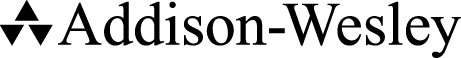
\includegraphics{AWlogoTitlePage-Mac}\\   % AW Mac
%\includegraphics{AWlogoTitlePage_PC}  \\  %AW PC
{\footnotesize 
Boston~$\bullet$~Columbus~$\bullet$~Indianapolis~$\bullet$~New York~$\bullet$~San Francisco~$\bullet$~Amsterdam~$\bullet$~Cape Town\\[1ex]
Dubai~$\bullet$~London~$\bullet$~Madrid~$\bullet$~Milan~$\bullet$~Munich~$\bullet$~Paris~$\bullet$~Montreal~$\bullet$~Toronto~$\bullet$~Delhi~$\bullet$~Mexico City\\[1ex]
Sao Paulo~$\bullet$~Sidney~$\bullet$~Hong Kong~$\bullet$~Seoul~$\bullet$~Singapore~$\bullet$~Taipei~$\bullet$~Tokyo\\[1ex]
}
\end{center}                               % The title page
%\thispagestyle{empty}
\vspace*{\fill}
{\footnotesize\raggedright 
\noindent Many of the designations used by manufacturers and sellers to distinguish their products are claimed as trademarks. Where those designations appear in this book, and the publisher was aware of a trademark claim, the designations have been printed with initial capital letters or in all capitals.\\
\hspace{\fill}\\
\noindent The authors and publisher have taken care in the preparation of this book, but make no expressed or implied warranty of any kind and assume no responsibility for errors or omissions. No liability is assumed for incidental or consequential damages in connection with or arising out of the use of the information or programs contained herein.\\   % change to authors (plural) if this book has multiple authors
\hspace{\fill}\\
\noindent For information about buying this title in bulk quantities, or for special sales opportunities (which may include electronic versions; custom cover designs; and content particular to your business, training goals, marketing focus, or branding interests), please contact our corporate sales department\linebreak[4] at \mbox{corpsales}@\mbox{pearsoned.com} or (800) 382-3419.\\
\hspace{\fill}\\
\noindent For government sales inquiries, please contact governmentsales@pearsoned.com.\\
\hspace{\fill}\\
\noindent For questions about sales outside the U.S., please contact intlcs@pearson.com.\\
\hspace{\fill}\\
\noindent Visit us on the Web: informit.com/aw\\     % use this line if you are publishing with AW
%\noindent Visit us on the Web: informit.com/ph\\   % use this line if you are publishing with PH
\hspace{\fill}\\
\noindent Library of Congress Control Number: TO COME FROM ITP\\  % update this with info provided by your production editor
\hspace{\fill}\\
\noindent Copyright~\copyright~2021 Pearson Education, Inc.\\
\hspace{\fill}\\
\noindent Cover image: [TO COME FROM ITP]\\
\hspace*{\fill}\\
\noindent All rights reserved. This publication is protected by copyright, and permission must be obtained from the publisher prior to any prohibited reproduction, storage in a retrieval system, or transmission in any form or by any means, electronic, mechanical, photocopying, recording, or likewise. For information regarding permissions, request forms and the appropriate contacts within the Pearson Education Global Rights \& Permissions Department, please visit www.pearson.com/permissions.\\
\hspace*{\fill}\\
\noindent ISBN-13: 978-0-13-738035-0\\[-.5ex] % update this with info provided by your production editor 
\noindent ISBN-10: 0-13-738035-6 \\ % update this with info provided by your production editor
\hspace*{\fill}\\
\noindent{\sf ScoutAutomatedPrintCode}
%\noindent Text printed in the United States on recycled paper at PRINTER INFO HERE.\\[-.5ex] % update this with info provided by your production editor
%\noindent First printing, MONTH YEAR % update this with info provided by your production editor
}                                % The cataloging-in-publication page
%\thispagestyle{empty}
\begin{center}The lines of text of the dedication will be broken\\ 
with the help of the production team\\ 
to ensure an attractive\\
layout.\\[1ex] 
Author Initials\\
\vspace*{3pc}
Should there be a second author, that author's lines of\\  % These lines are 
dedication text will go here and will also be broken\\        % commented out 
in whatever way is attractive and logical.\\[1ex]                % if unneeded.
Author Initials\\
\end{center}                      % The dedication page
%\cleardoublepage
%\parskip .5ex                       % Add space between Contents items
%\tableofcontents                  % Make the Table of Contents 
%\cleardoublepage                
%\parskip 0in                         % Reset to zero interpar spacing
%\cleardoublepage
\chapter*{Foreword}
\markboth{Foreword}{Foreword}

The text of the foreword will go here.                 % Add foreword
%\cleardoublepage
\chapter*{Preface}

The text of the preface will go here.  All the elements and commands offered within the text will work here as well. 

Sed ut perspiciatis unde omnis iste natus error sit voluptatem accusantium doloremque laudantium, totam rem aperiam, eaque ipsa quae ab illo inventore veritatis et quasi architecto beatae vitae dicta sunt explicabo. Nemo enim ipsam voluptatem quia voluptas sit aspernatur aut odit aut fugit, sed quia consequuntur magni dolores eos qui ratione voluptatem sequi nesciunt. Neque porro quisquam est, qui dolorem ipsum quia dolor sit amet, consectetur, adipisci velit, sed quia non numquam eius modi tempora incidunt ut labore et dolore magnam aliquam quaerat voluptatem. Ut enim ad minima veniam, quis nostrum exercitationem ullam corporis suscipit laboriosam, nisi ut aliquid ex ea commodi consequatur? Quis autem vel eum iure reprehenderit qui in ea voluptate velit esse quam nihil molestiae consequatur, vel illum qui dolorem eum fugiat quo voluptas nulla pariatur? 

At vero eos et accusamus et iusto odio dignissimos ducimus qui blanditiis praesentium voluptatum deleniti atque corrupti quos dolores et quas molestias excepturi sint occaecati cupiditate non provident, similique sunt in culpa qui officia deserunt mollitia animi, id est laborum et dolorum fuga. Et harum quidem rerum facilis est et expedita distinctio. Nam libero tempore, cum soluta nobis est eligendi optio cumque nihil impedit quo minus id quod maxime placeat facere possimus, omnis voluptas assumenda est, omnis dolor repellendus. Temporibus autem quibusdam et aut officiis debitis aut rerum necessitatibus saepe eveniet ut et voluptates repudiandae sint et molestiae non recusandae. Itaque earum rerum hic tenetur a sapiente delectus, ut aut reiciendis voluptatibus maiores alias consequatur aut perferendis doloribus asperiores repellat.

Sed ut perspiciatis unde omnis iste natus error sit voluptatem accusantium doloremque laudantium, totam rem aperiam, eaque ipsa quae ab illo inventore veritatis et quasi architecto beatae vitae dicta sunt explicabo. Nemo enim ipsam voluptatem quia voluptas sit aspernatur aut odit aut fugit, sed quia consequuntur magni dolores eos qui ratione voluptatem sequi nesciunt.Neque porro quisquam est, qui dolorem ipsum quia dolor sit amet, consectetur, adipisci velit, sed quia non numquam eius modi tempora incidunt ut labore et dolore magnam aliquam quaerat voluptatem. Ut enim ad minima veniam, quis nostrum exercitationem ullam corporis suscipit laboriosam, nisi ut aliquid ex ea commodi consequatur? Quis autem vel eum iure reprehenderit qui in ea voluptate velit esse quam nihil molestiae consequatur, vel illum qui dolorem eum fugiat quo voluptas nulla pariatur? 

At vero eos et accusamus et iusto odio dignissimos ducimus qui blanditiis praesentium voluptatum deleniti atque corrupti quos dolores et quas molestias excepturi sint occaecati cupiditate non provident, similique sunt in culpa qui officia deserunt mollitia animi, id est laborum et dolorum fuga. Et harum quidem rerum facilis est et expedita distinctio. Nam libero tempore, cum soluta nobis est eligendi optio cumque nihil impedit quo minus id quod maxime placeat facere possimus, omnis voluptas assumenda est, omnis dolor repellendus. Temporibus autem quibusdam et aut officiis debitis aut rerum necessitatibus saepe eveniet ut et voluptates repudiandae sint et molestiae non recusandae. Itaque earum rerum hic tenetur a sapiente delectus, ut aut reiciendis voluptatibus maiores alias consequatur aut perferendis doloribus asperiores repellat.

Sed ut perspiciatis unde omnis iste natus error sit voluptatem accusantium doloremque laudantium, totam rem aperiam, eaque ipsa quae ab illo inventore veritatis et quasi architecto beatae vitae dicta sunt explicabo. Nemo enim ipsam voluptatem quia voluptas sit aspernatur aut odit aut fugit, sed quia consequuntur magni dolores eos qui ratione voluptatem sequi nesciunt.Neque porro quisquam est, qui dolorem ipsum quia dolor sit amet, consectetur, adipisci velit, sed quia non numquam eius modi tempora incidunt ut labore et dolore magnam aliquam quaerat voluptatem. Ut enim ad minima veniam, quis nostrum exercitationem ullam corporis suscipit laboriosam, nisi ut aliquid ex ea commodi consequatur? Quis autem vel eum iure reprehenderit qui in ea voluptate velit esse quam nihil molestiae consequatur, vel illum qui dolorem eum fugiat quo voluptas nulla pariatur? 

At vero eos et accusamus et iusto odio dignissimos ducimus qui blanditiis praesentium voluptatum deleniti atque corrupti quos dolores et quas molestias excepturi sint occaecati cupiditate non provident, similique sunt in culpa qui officia deserunt mollitia animi, id est laborum et dolorum fuga. Et harum quidem rerum facilis est et expedita distinctio. Nam libero tempore, cum soluta nobis est eligendi optio cumque nihil impedit quo minus id quod maxime placeat facere possimus, omnis voluptas assumenda est, omnis dolor repellendus. Temporibus autem quibusdam et aut officiis debitis aut rerum necessitatibus saepe eveniet ut et voluptates repudiandae sint et molestiae non recusandae. Itaque earum rerum hic tenetur a sapiente delectus, ut aut reiciendis voluptatibus maiores alias consequatur aut perferendis doloribus asperiores repellat.

Sed ut perspiciatis unde omnis iste natus error sit voluptatem accusantium doloremque laudantium, totam rem aperiam, eaque ipsa quae ab illo inventore veritatis et quasi architecto beatae vitae dicta sunt explicabo. Nemo enim ipsam voluptatem quia voluptas sit aspernatur aut odit aut fugit, sed quia consequuntur magni dolores eos qui ratione voluptatem sequi nesciunt. Neque porro quisquam est, qui dolorem ipsum quia dolor sit amet, consectetur, adipisci velit, sed quia non numquam eius modi tempora incidunt ut labore et dolore magnam aliquam quaerat voluptatem. Ut enim ad minima veniam, quis nostrum exercitationem ullam corporis suscipit laboriosam, nisi ut aliquid ex ea commodi consequatur? Quis autem vel eum iure reprehenderit qui in ea voluptate velit esse quam nihil molestiae consequatur, vel illum qui dolorem eum fugiat quo voluptas nulla pariatur? 

At vero eos et accusamus et iusto odio dignissimos ducimus qui blanditiis praesentium voluptatum deleniti atque corrupti quos dolores et quas molestias excepturi sint occaecati cupiditate non provident, similique sunt in culpa qui officia deserunt mollitia animi, id est laborum et dolorum fuga. Et harum quidem rerum facilis est et expedita distinctio. Nam libero tempore, cum soluta nobis est eligendi optio cumque nihil impedit quo minus id quod maxime placeat facere possimus, omnis voluptas assumenda est, omnis dolor repellendus. Temporibus autem quibusdam et aut officiis debitis aut rerum necessitatibus saepe eveniet ut et voluptates repudiandae sint et molestiae non recusandae. Itaque earum rerum hic tenetur a sapiente delectus, ut aut reiciendis voluptatibus maiores alias consequatur aut perferendis doloribus asperiores repellat.


Sed ut perspiciatis unde omnis iste natus error sit voluptatem accusantium doloremque laudantium, totam rem aperiam, eaque ipsa quae ab illo inventore veritatis et quasi architecto beatae vitae dicta sunt explicabo. Nemo enim ipsam voluptatem quia voluptas sit aspernatur aut odit aut fugit, sed quia consequuntur magni dolores eos qui ratione voluptatem sequi nesciunt. Neque porro quisquam est, qui dolorem ipsum quia dolor sit amet, consectetur, adipisci velit, sed quia non numquam eius modi tempora incidunt ut labore et dolore magnam aliquam quaerat voluptatem. Ut enim ad minima veniam, quis nostrum exercitationem ullam corporis suscipit laboriosam, nisi ut aliquid ex ea commodi consequatur? Quis autem vel eum iure reprehenderit qui in ea voluptate velit esse quam nihil molestiae consequatur, vel illum qui dolorem eum fugiat quo voluptas nulla pariatur? 

At vero eos et accusamus et iusto odio dignissimos ducimus qui blanditiis praesentium voluptatum deleniti atque corrupti quos dolores et quas molestias excepturi sint occaecati cupiditate non provident, similique sunt in culpa qui officia deserunt mollitia animi, id est laborum et dolorum fuga. Et harum quidem rerum facilis est et expedita distinctio. Nam libero tempore, cum soluta nobis est eligendi optio cumque nihil impedit quo minus id quod maxime placeat facere possimus, omnis voluptas assumenda est, omnis dolor repellendus. Temporibus autem quibusdam et aut officiis debitis aut rerum necessitatibus saepe eveniet ut et voluptates repudiandae sint et molestiae non recusandae. Itaque earum rerum hic tenetur a sapiente delectus, ut aut reiciendis voluptatibus maiores alias consequatur aut perferendis doloribus asperiores repellat.


Sed ut perspiciatis unde omnis iste natus error sit voluptatem accusantium doloremque laudantium, totam rem aperiam, eaque ipsa quae ab illo inventore veritatis et quasi architecto beatae vitae dicta sunt explicabo. Nemo enim ipsam voluptatem quia voluptas sit aspernatur aut odit aut fugit, sed quia consequuntur magni dolores eos qui ratione voluptatem sequi nesciunt. Neque porro quisquam est, qui dolorem ipsum quia dolor sit amet, consectetur, adipisci velit, sed quia non numquam eius modi tempora incidunt ut labore et dolore magnam aliquam quaerat voluptatem. Ut enim ad minima veniam, quis nostrum exercitationem ullam corporis suscipit laboriosam, nisi ut aliquid ex ea commodi consequatur? Quis autem vel eum iure reprehenderit qui in ea voluptate velit esse quam nihil molestiae consequatur, vel illum qui dolorem eum fugiat quo voluptas nulla pariatur? 

At vero eos et accusamus et iusto odio dignissimos ducimus qui blanditiis praesentium voluptatum deleniti atque corrupti quos dolores et quas molestias excepturi sint occaecati cupiditate non provident, similique sunt in culpa qui officia deserunt mollitia animi, id est laborum et dolorum fuga. Et harum quidem rerum facilis est et expedita distinctio. Nam libero tempore, cum soluta nobis est eligendi optio cumque nihil impedit quo minus id quod maxime placeat facere possimus, omnis voluptas assumenda est, omnis dolor repellendus. Temporibus autem quibusdam et aut officiis debitis aut rerum necessitatibus saepe eveniet ut et voluptates repudiandae sint et molestiae non recusandae. Itaque earum rerum hic tenetur a sapiente delectus, ut aut reiciendis voluptatibus maiores alias consequatur aut perferendis doloribus asperiores repellat.
                 % Add preface 
%\cleardoublepage
\chapter*{Acknowledgements}

\noindent The text of the author's acknowledgements will go here.                         % Add acknowledgements 
%\cleardoublepage
\chapter*{About the Authors}

 % wrapfig doesn't like to be immediately after a chapter/section command 
 % so we are tricking it a bit with the \hspace and the \par commands.
\hspace*{\fill}\\  
\par\begin{wrapfigure}[12]{L}[0pt]{0pt}
\includegraphics{AuthorPhoto}\end{wrapfigure}\noindent AUTHOR BIO WILL APPEAR HERE.  Lorem ipsum dolor sit amet, consectetur adipisicing elit, sed do eiusmod tempor incididunt ut labore et dolore magna aliqua. Ut enim ad minim veniam, quis nostrud exercitation ullamco laboris nisi ut aliquip ex ea commodo consequat. Duis aute irure dolor in reprehenderit in voluptate velit esse cillum dolore eu fugiat nulla pariatur. Excepteur sint occaecat cupidatat non proident, sunt in culpa qui officia deserunt mollit anim id est laborum. Lorem ipsum dolor sit amet, consectetur adipisicing elit, sed do eiusmod tempor incididunt ut labore et dolore magna aliqua. Ut enim ad minim veniam, quis nostrud exercitation ullamco laboris nisi ut aliquip ex ea commodo consequat. Lorem ipsum dolor sit amet, consectetur adipisicing elit, sed do eiusmod tempor incididunt ut labore et dolore magna aliqua. Ut enim ad minim veniam, quis nostrud exercitation ullamco laboris nisi ut aliquip ex ea commodo consequat. 

\vspace*{18pt} % we add some space for a nice layout
\begin{wrapfigure}[12]{L}[0pt]{0pt}
\includegraphics{AuthorPhoto}\end{wrapfigure} \noindent AUTHOR BIO WILL APPEAR HERE.  Lorem ipsum dolor sit amet, consectetur adipisicing elit, sed do eiusmod tempor incididunt ut labore et dolore magna aliqua. Ut enim ad minim veniam, quis nostrud exercitation ullamco laboris nisi ut aliquip ex ea commodo consequat. Duis aute irure dolor in reprehenderit in voluptate velit esse cillum dolore eu fugiat nulla pariatur. Excepteur sint occaecat cupidatat non proident, sunt in culpa qui officia deserunt mollit anim id est laborum. Lorem ipsum dolor sit amet, consectetur adipisicing elit, sed do eiusmod tempor incididunt ut labore et dolore magna aliqua. Ut enim ad minim veniam, quis nostrud exercitation ullamco laboris nisi ut aliquip ex ea commodo consequat. Lorem ipsum dolor sit amet, consectetur adipisicing elit, sed do eiusmod tempor incididunt ut labore et dolore magna aliqua. Ut enim ad minim veniam, quis nostrud exercitation ullamco laboris nisi ut aliquip ex ea commodo consequat. 
                   % Add about the author page
\cleardoublepage                  
%%%%%%%The front matter ends


%%%%%%%%%% Now we'll start on the main text for the book.  
%% Main Text:
\pagenumbering{arabic}		  % Arabic numbering
%\part{This is the Part Title}
\vspace*{4pt}
\sffamily % this sets this page in sans serif font

\noindent Chapter \ref{ExampleChap}, "\titleref{ExampleChap},"  is followed by a one-sentence description of each chapter. 

Chapter \ref{samplechap2}, "\titleref{samplechap2},"  is followed by a one-sentence description of each chapter and if the sentence is longer what happens when it runs to two lines.

Chapter \ref{samplechap3}, "\titleref{samplechap3}," is followed by a one-sentence description of each chapter and if the sentence is longer what happens when it runs to two lines. 

\normalfont % this resets the fonts to our normal settings




            % Part I
Chapterhead does not count in the Level counting; it is its own separate thing

\section[C++xx with {\tt Code}]{C++xx with {\SecCode Code}--- This is a Level 1 Head} 

\subsection[{\tt auto}]{{\SubsecCode auto} --- This is a Level 2 Head}

text here

\subsubsection[Description with {\tt Code}]{Description with {\SubsubsecCode Code} --- This is a Level 3 Head}

text here

\begin{leftbar}
{And now we need to make sure the Example will flow nicely across pages.  Phasellus nibh lectus, lacinia vitae mollis at, lobortis lobortis sapien. Phasellus vestibulum mi sit amet ante pulvinar mattis. Praesent rhoncus iaculis metus at faucibus. Maecenas in sem et mauris scelerisque scelerisque eget vel neque. In placerat pharetra nisi sit amet vestibulum. See Listing \ref{listingexample} for a listing with a title. 
% this is the code for a listing with a title and a number. 
\begin{lstlisting}[caption={This is the Listing Title.},label={listingexample},frame=tb]
Now a bit more code, with a title and a number and some
lines to set it off             
\end{lstlisting}
\begin{lstlisting}[caption={And if the title is long enough to run over two lines, then it is set flushleft rather than centered.},label={listingexample},frame=tb]
Now a bit more code, with a longer title 
123456789A123456789B123456789C123456789D123456789E123456789F123456789G123456789H
Testing the line length           
\end{lstlisting}
Sed faucibus rhoncus nisl id dignissim. Quisque sed metus justo. Aliquam aliquet molestie condimentum. Nulla ac libero tellus. }
\end{leftbar}
and then testing a listing outside of the Example environment.\cprotect\footnote{\textbf{lakos20},
  section 0.5, pp 34-42

 \begin{lstlisting}[language=C++, label={ testlabel },basicstyle={\footnotesize\tt}]
  template <typename Range>
  auto sortRangeImpl(Range& range, int) -> decltype(range.sort(), void());
      // The comma operator is used to force the return type to `void`,
      // regardless of the return type of `range.sort()`.

  template <typename Range, typename = decltype(std::declval<Range&>().sort()>
  auto sortRangeImpl(Range& range, int);
      // `std::declval` is used to generate a reference to `Range` that can be
      // used in an unevaluated expression
  \end{lstlisting}
      } Maybe we don't want to use the Example environment. 
\begin{lstlisting}[caption={Caption.},label={listingexample},frame=tb]
Now a bit more code, with a longer title 
123456789A123456789B123456789C123456789D123456789E123456789F123456789G123456789H
Testing the line length           
\end{lstlisting}

\subsubsection{Potential Pitfalls}

\paragraph[Performance Concerns with {\tt Code}]{Performance Concerns with {\ParaCode Code} --- This is a Level 4 Head}

\paragraph{Issues at Scale}

\paragraph{Language/Feature Deficiencies}

\paragraph{Annoyances}

\paragraph{Related Information}

\paragraph{See Also}

\paragraph{Further Reading}


  % Chapter 1
%% This file should contain the full glossary contents


\newglossaryentry{ABI}{
  name={ABI},
  description={
TODO
}}

\newglossaryentry{abstract interface}{
  name={Abstract Interface},
  description={
TODO
}}


\newglossaryentry{access modifier}{
  name={Access Modifier},
  description={
TODO
}}

\newglossaryentry{access specifier}{
  name={Access Specifier},
  description={
TODO
}}

\newglossaryentry{acquire/release memory barrier}{
  name={Acquire/Release Memory Barrier},
  description={
TODO
}}

\newglossaryentry{aggregate}{
  name={Aggregate},
  description={
TODO
}}

\newglossaryentry{aggregate initialization}{
  name={Aggregate Initialization},
  description={
TODO
}}

\newglossaryentry{algebra}{
  name={Algebra},
  description={
TODO
}}

\newglossaryentry{alias template}{
  name={Alias Template},
  description={
TODO
}}

\newglossaryentry{alignment}{
  name={Alignment},
  description={
TODO
}}

\newglossaryentry{alignment requirement}{
  name={Alignment Requirement},
  description={
TODO
}}

\newglossaryentry{API}{
  name={API},
  description={
TODO
}}

\newglossaryentry{architectural insulation}{
  name={Architectural Insulation},
  description={
TODO
}}

\newglossaryentry{argument-dependent lookup (ADL)}{
  name={Argument-Dependent Lookup (ADL)},
  description={
TODO
}}


\newglossaryentry{arithmetic type}{
  name={Arithmetic Type},
  description={
TODO
}}

\newglossaryentry{array to pointer decay}{
  name={Array To Pointer Decay},
  description={
TODO
}}


\newglossaryentry{array type}{
  name={Array Type},
  description={
TODO
}}

\newglossaryentry{atomic}{
  name={Atomic},
  description={
TODO
}}

\newglossaryentry{Automatic}{
  name={Automatic},
  description={
TODO
}}

\newglossaryentry{automatic}{
  name={Automatic},
  description={
TODO
}}

\newglossaryentry{automatic storage duration}{
  name={Automatic Storage Duration},
  description={
TODO
}}

\newglossaryentry{automatic variable}{
  name={automatic variable},
  description={
TODO
}}

\newglossaryentry{B0}{
  name={B0},
  description={
TODO
}}

\newglossaryentry{barriers}{
  name={Barriers},
  description={
TODO
}}

\newglossaryentry{base name}{
  name={Base Name},
  description={
TODO
}}

\newglossaryentry{basic source character set}{
  name={Basic Source Character Set},
  description={
TODO
}}

\newglossaryentry{benchmark test}{
  name={Benchmark Test},
  description={
TODO
}}

\newglossaryentry{block scope}{
  name={Block Scope},
  description={
TODO
}}

\newglossaryentry{boilerplate code}{
  name={Boilerplate Code},
  description={
TODO
}}

\newglossaryentry{brace elision}{
  name={Brace Elision},
  description={
TODO
}}

\newglossaryentry{braced initialization}{
  name={Brace Initialization},
  description={
TODO
}}

\newglossaryentry{bytes}{
  name={Bytes},
  description={
TODO
}}

\newglossaryentry{C style function}{
  name={C-Style Function},
  description={
TODO
}}

\newglossaryentry{cache hit}{
  name={Cache Hit},
  description={
TODO
}}

\newglossaryentry{cache line}{
  name={Cache Line},
  description={
TODO
}}

\newglossaryentry{cache miss}{
  name={Cache Miss},
  description={
TODO
}}

\newglossaryentry{call operator}{
  name={Call Operator},
  description={
TODO
}}

\newglossaryentry{callable object}{
  name={Callable Object},
  description={
TODO
}}

\newglossaryentry{callback functions}{
  name={Callback Functions},
  description={
TODO
}}

\newglossaryentry{capture default}{
  name={Capture Default},
  description={
TODO
}}

\newglossaryentry{capture init}{
  name={Capture Init},
  description={
TODO
}}

\newglossaryentry{captured by copy}{
  name={Captured By Copy},
  description={
TODO
}}

\newglossaryentry{captured by reference}{
  name={Captured By Reference},
  description={
TODO
}}

\newglossaryentry{captured variable}{
  name={Captured Variable},
  description={
TODO
}}

\newglossaryentry{carry dependency}{
  name={Carry Dependecy},
  description={
TODO
}}

\newglossaryentry{cast}{
  name={Cast},
  description={
TODO
}}

\newglossaryentry{character literal}{
  name={Character Literal},
  description={
TODO
}}


\newglossaryentry{CI}{
  name={CI},
  description={
TODO
}}

\newglossaryentry{class member access expression}{
  name={Class Member Access Expression},
  description={
TODO (include any expression that is used to refer to a class member, such as \texttt{object.member}, \texttt{object->member}, \texttt{object.*member}.)
}}

\newglossaryentry{class template argument deduction}{
  name={Class Template Argument Deduction},
  description={
TODO 
}}

\newglossaryentry{closure}{
  name={Closure},
  description={
TODO
}}

\newglossaryentry{closure object}{
  name={Closure Object},
  description={
TODO
}}

\newglossaryentry{closure type}{
  name={Closure Type},
  description={
TODO
}}

\newglossaryentry{code bloat}{
  name={Code Bloat},
  description={
TODO
}}

\newglossaryentry{Collatz function}{
  name={Collatz Function},
  description={
TODO
}}

\newglossaryentry{Collatz length}{
  name={Collatz Length},
  description={
TODO
}}

\newglossaryentry{Collatz sequence}{
  name={Collatz Sequence},
  description={
TODO
}}

\newglossaryentry{compile time constant}{
  name={Compile-Time Constant},
  description={
TODO
}}

\newglossaryentry{compile time coupling}{
  name={Compile-Time Coupling},
  description={
TODO
}}

\newglossaryentry{compile time dispatch}{
  name={Compile-Time Dispatch},
  description={
TODO
}}

\newglossaryentry{complete type}{
  name={Complete Type},
  description={
TODO
}}

\newglossaryentry{component}{
  name={Component},
  description={
TODO
}}

\newglossaryentry{component local}{
  name={Component Local},
  description={
TODO
}}

\newglossaryentry{components}{
  name={Components},
  description={
TODO
}}

\newglossaryentry{concepts}{
  name={Concepts},
  description={
TODO
}}

\newglossaryentry{concrete class}{
  name={Concrete Class},
  description={
An expression that can be evaluated at compile time.  Mention \texttt{constexpr} and state that \texttt{const} variables that are initialized from a compile-time constants are themselves required to be compile-time constants.  New info to me in June 2020, worthwhile to have. 
}}

\newglossaryentry{conditionally supported}{
  name={Conditionally Supported},
  description={
TODO
}}

\newglossaryentry{const default constructible}{
  name={const Default Constructible},
  description={
TODO
}}

\newglossaryentry{constant expression}{
  name={Constant Expression},
  description={
TODO
}}

\newglossaryentry{constant initialization}{
  name={Constant Initialization},
  description={
TODO
}}

\newglossaryentry{constexpr context}{
  name={Constexpr Context},
  description={
TODO
}}

\newglossaryentry{contextual convertibility to bool}{
  name={Contextual Convertibility to \texttt{bool}},
  description={
TODO
}}

\newglossaryentry{contextual keyword}{
  name={Contextual Keyword},
  description={
A \textit{contextual keyword} is a special identifier that acts like a \textit{keyword} when used in particular contexts. \texttt{override} is an example as it can be used as a regular identifier outside of member-function declarators.
}}

\newglossaryentry{continuous refactoring}{
  name={Continuous Refactoring},
  description={
TODO
}}

\newglossaryentry{contract}{
  name={Contract},
  description={
TODO
}}

\newglossaryentry{conventional string literals}{
  name={Conventional String Literals},
  description={
TODO
}}

\newglossaryentry{converting constructors}{
  name={Converting Constructors},
  description={
TODO
}}

\newglossaryentry{conversion operators}{
  name={Conversion Operators},
  description={
TODO
}}

\newglossaryentry{cookie}{
  name={Cookie},
  description={
TODO
}}

\newglossaryentry{copy}{
  name={Copy},
  description={
TODO
}}

\newglossaryentry{copy assignment operator}{
  name={Copy Assignment Operator},
  description={
TODO
}}

\newglossaryentry{copy constructor}{
  name={Copy Constructor},
  description={
TODO
}}

\newglossaryentry{copy direct}{
  name={Copy/Direct},
  description={
TODO
}}

\newglossaryentry{copy elision}{
  name={Copy Elision},
  description={
TODO
}}

\newglossaryentry{copy initialization}{
  name={Copy Initialization},
  description={
TODO
}}

\newglossaryentry{copy initialized}{
  name={Copy Initialize},
  description={
TODO
}}

\newglossaryentry{copy list}{
  name={Copy List},
  description={
TODO
}}

\newglossaryentry{copy list initialization}{
  name={Copy List Initialization},
  description={
TODO
}}

\newglossaryentry{copy operations}{
  name={Copy Operations},
  description={
TODO
}}

\newglossaryentry{copy semantics}{
  name={Copy Semantics},
  description={
An operation on two objects, a destination and a source, has {\romeoglossfont copy semantics}
if, after it completes, the {\romeoglossfont value} of the source object remains unchanged and the target object
has the same {\romeoglossfont value} as does the source.   ..  for some criteria the source and destination are
the same, for a value semantic type that property is value...
}}

\newglossaryentry{critical section}{
  name={Critical Section},
  description={
TODO
}}

\newglossaryentry{curiously recurring template pattern (CRTP)}{
  name={Curiously Recurring Template Pattern (CRTP)},
  description={
TODO
}}

\newglossaryentry{currying}{
  name={Currying},
  description={
TODO
}}

\newglossaryentry{cv qualifiers}{
  name={CV-Qualifiers},
  description={
TODO
}}

\newglossaryentry{cyclic physical dependency}{
  name={Cyclic Physical Dependency},
  description={
TODO
}}

\newglossaryentry{cyclically dependent}{
  name={Cyclically Dependent},
  description={
TODO
}}

\newglossaryentry{data dependency}{
  name={Data Dependency},
  description={
TODO
}}

\newglossaryentry{data dependency chain}{
  name={Data Dependency Chain},
  description={
TODO
}}

\newglossaryentry{data member}{
  name={Data Member},
  description={
TODO
}}

\newglossaryentry{data races}{
  name={Data Races},
  description={
TODO
}}

\newglossaryentry{decimal floating point}{
  name={Decimal Floating-Point},
  description={
TODO
}}

\newglossaryentry{declaration}{
  name={Declaration},
  description={
TODO
}}

\newglossaryentry{declare}{
  name={Declare},
  description={
TODO
}}

\newglossaryentry{declared type}{
  name={Declared Type},
  description={
TODO The type of the *entity* named by the given expression.
}}

\newglossaryentry{declared interface}{
  name={Declared Interface},
  description={
TODO
}}

\newglossaryentry{declaring}{
  name={Declaring},
  description={
TODO
}}

\newglossaryentry{deduced return type}{
  name={Deduced Return Type},
  description={
TODO
}}

\newglossaryentry{default initialization}{
  name={Default Initialization},
  description={
TODO
}}

\newglossaryentry{default initialized}{
  name={Default Initialized},
  description={
TODO
}}

\newglossaryentry{default value}{
  name={Default/Value},
  description={
TODO
}}

\newglossaryentry{defensive}{
  name={Defensive},
  description={
TODO
}}

\newglossaryentry{define}{
  name={Define},
  description={
TODO
}}

\newglossaryentry{definition}{
  name={Definition},
  description={
TODO
}}

\newglossaryentry{delegating constructor}{
  name={Delegating Constructor},
  description={
TODO
}}

\newglossaryentry{delete}{
  name={Delete},
  description={
TODO
}}

\newglossaryentry{deleted function}{
  name={Deleted Function},
  description={
TODO
}}

\newglossaryentry{dependent type}{
  name={Dependent Type},
  description={
TODO
}}

\newglossaryentry{design pattern}{
  name={Design Pattern},
  description={
TODO
}}

\newglossaryentry{diffusion}{
  name={Diffusion},
  description={
TODO
}}

\newglossaryentry{dimensional unit type}{
  name={Dimensional Unit Type},
  description={
TODO
}}

\newglossaryentry{direct}{
  name={Direct},
  description={
TODO
}}


\newglossaryentry{direct initialization}{
  name={Direct Initialization},
  description={
TODO
}}

\newglossaryentry{direct initialized}{
  name={Direct Initialized},
  description={
TODO
}}

\newglossaryentry{direct list}{
  name={Direct List},
  description={
TODO
}}

\newglossaryentry{direct list initialization}{
  name={Direct List Initialization},
  description={
TODO
}}

\newglossaryentry{direct mapped}{
  name={Direct Initialization},
  description={
TODO
}}

\newglossaryentry{disambiguator}{
  name={Disambiguator},
  description={
TODO
}}

\newglossaryentry{duck typing}{
  name={Duck Typing},
  description={
TODO
}}

\newglossaryentry{dumb data}{
  name={Dumb Data},
  description={
TODO
}}

\newglossaryentry{Eigen}{
  name={Eigen},
  description={
TODO
}}

\newglossaryentry{embedded development}{
  name={Embedded Development},
  description={
TODO
}}

\newglossaryentry{embedded systems}{
  name={Embedded Systems},
  description={
TODO
}}

\newglossaryentry{emplacement}{
  name={Emplacement},
  description={
TODO
}}

\newglossaryentry{empty base optimization}{
  name={Empty Base Optimization},
  description={
TODO
}}


\newglossaryentry{encapsulation}{
  name={Encapsulation},
  description={
TODO
}}

\newglossaryentry{encoding prefix}{
  name={Encoding Prefix},
  description={
TODO
}}

\newglossaryentry{entity}{
  name={Entity},
  description={
TODO
}}

\newglossaryentry{escalating}{
  name={Escalating},
  description={
TODO
}}

\newglossaryentry{exception specification}{
  name={Exception Specification},
  description={
TODO
}}

\newglossaryentry{excess n}{
  name={Excess $N$},
  description={
TODO
}}

\newglossaryentry{execution character set}{
  name={Execution Character Set},
  description={
TODO
}}

\newglossaryentry{explicit}{
  name={Explicit},
  description={
TODO
}}

\newglossaryentry{explicit instantiation declaration}{
  name={Explicit Instantiation Declaration},
  description={
TODO
}}

\newglossaryentry{explicit instantiation definition}{
  name={Explicit Instantiation Definition},
  description={
TODO
}}


\newglossaryentry{explicit instantiation directive}{
  name={Explicit Instantiation Directive},
  description={
TODO
}}


\newglossaryentry{explicit specifier}{
  name={\texttt{explicit} Specifier},
  description={
TODO
}}

\newglossaryentry{explicitly captured}{
  name={Explicitly Captured},
  description={
TODO
}}

\newglossaryentry{explicitly copied}{
  name={Explicitly Copied},
  description={
TODO
}}

\newglossaryentry{expression SFINAE}{
  name={Expression SFINAE},
  description={
TODO
}}

\newglossaryentry{expression template}{
  name={Expression Template},
  description={
Expression templates is a template
metaprogramming technique where the full structure of an expression is
represented with nested template instantiations allowing lazy
evaluation and certain optimizations. For example, this technique is
often utilized by linear algebra libraries, such as
  ``\emcppsgloss[Eigen]{Eigen}" (http://eigen.tuxfamily.org/).
}}

\newglossaryentry{extended alignment}{
  name={Extended Alignment},
  description={
TODO
}}

\newglossaryentry{factory function}{
  name={Factory Function},
  description={
TODO
}}

\newglossaryentry{factory operator}{
  name={Factory Operator},
  description={
TODO
}}

\newglossaryentry{false sharing}{
  name={false sharing},
  description={
TODO
}}


\newglossaryentry{fences}{
  name={Fences},
  description={
TODO
}}

\newglossaryentry{file extension}{
  name={File Extension},
  description={
TODO
}}

\newglossaryentry{floating point literal}{
  name={Floating Point Literal},
  description={
TODO
}}

\newglossaryentry{floating-point-to-integer conversion}{
  name={Floating-Point-to-Integer Conversion},
  description={
TODO
}}

\newglossaryentry{flow of control}{
  name={Flow Of Control},
  description={
TODO
}}

\newglossaryentry{footprint}{
  name={Footprint},
  description={
TODO
}}

\newglossaryentry{for range declaration}{
  name={For Range Declaration},
  description={
TODO
}}

\newglossaryentry{forward class declaration}{
  name={Forward Class Declaration},
  description={
TODO
}}

\newglossaryentry{forward declaration}{
  name={Forward Declaration},
  description={
TODO
}}

\newglossaryentry{forward declare}{
  name={Forward Declare},
  description={
TODO
}}

\newglossaryentry{forward declared}{
  name={Forward Declared},
  description={
TODO
}}

\newglossaryentry{forwarding reference}{
  name={Forwarding Reference},
  description={
TODO
}}

\newglossaryentry{fragmentation}{
  name={Fragmentation},
  description={
TODO
}}

\newglossaryentry{free function}{
  name={Free Function},
  description={
TODO
}}

\newglossaryentry{free operator}{
  name={Free Operator},
  description={
TODO
}}

\newglossaryentry{full expression}{
  name={Full Expression},
  description={
TODO
}}

\newglossaryentry{full specialization}{
  name={Full Specialization},
  description={
TODO
}}

\newglossaryentry{fully associative}{
  name={Fully Associative},
  description={
TODO
}}

\newglossaryentry{fully constructed}{
  name={Fully Constructed},
  description={
TODO
}}

\newglossaryentry{function object}{
  name={Function Object},
  description={
TODO
}}

\newglossaryentry{function scope}{
  name={Function Scope},
  description={
TODO
}}

\newglossaryentry{function template argument type deduction}{
  name={Function Template Argument Type Deduction},
  description={
TODO
}}

\newglossaryentry{functor}{
  name={Functor},
  description={
TODO
}}

\newglossaryentry{functor class}{
  name={Functor Class},
  description={
TODO
}}

\newglossaryentry{functor type}{
  name={Functor Type},
  description={
TODO
}}

\newglossaryentry{fundamental alignment}{
  name={Fundamental Alignment},
  description={
TODO
}}

\newglossaryentry{fundamental integral type}{
  name={Fundamental Integral Type},
  description={
TODO
}}

\newglossaryentry{fundamental integral types}{
  name={Fundamental Integral Types},
  description={
TODO
}}

\newglossaryentry{fundamental type}{
  name={Fundamental Type},
  description={
TODO
}}

\newglossaryentry{garbage value}{
  name={Garbage Value},
  description={
TODO
}}

\newglossaryentry{general purpose machines}{
  name={General Purpose Machines},
  description={
General-purpose machines are what Big Tech, the financial industry, and many other large companies use exclusively.
}}

\newglossaryentry{generic lambda}{
  name={Generic Lambda},
  description={
TODO
}}

\newglossaryentry{golden file}{
  name={Golden File},
  description={
TODO
}}

\newglossaryentry{golden output}{
  name={Golden Output},
  description={
TODO
}}

\newglossaryentry{header-only library}{
  name={Header-Only Library},
  description={
TODO
}}

\newglossaryentry{hide}{
  name={Hide or Hiding},
  alts={{hiding},
       },
  description={
Function-name \textbf{hiding} occurs when a member function in a derived class has the same name as one in the base class, but it is not overriding it due to a difference in the function signature or because the member function in the base class is not \texttt{virtual}. The hidden member function will \textbf{not} participate in dynamic dispatch; the member function of the base class will be invoked instead when invoked via a pointer or reference to the base class . The same code would have invoked the derived class's implementation had the member function of the base class had been \textbf{overridden} rather than \textbf{hidden}.
}}

\newglossaryentry{higher order function}{
  name={Higher-Order Function},
  description={
TODO
}}

\newglossaryentry{Hyrum's law}{
  name={Hyrum's Law},
  description={
TODO
}}

\newglossaryentry{IFNDR}{
  name={IFNDR},
  description={
TODO
}}

\newglossaryentry{id expression}{
  name={Id Expression},
  description={
TODO are most commonly \textbf{Identifiers}; other forms include overloaded operator names (in function notation), names of user-defined-conversion or literal operators, and destructor names, and ??template names followed by their argument lists??.
}}

\newglossaryentry{ill formed}{
  name={Ill Formed},
  description={
TODO
}}

\newglossaryentry{ill formed, no diagnostic required (IFNDR)}{
  name={Ill Formed, No Diagnostic Required  (IFNDR)},
  description={
TODO
}}

\newglossaryentry{imperative}{
  name={Imperative},
  description={
TODO
}}

\newglossaryentry{implementation defined}{
  name={Implementation Defined},
  description={
TODO
}}

\newglossaryentry{implementation inheritance}{
  name={Implementation Inheritance},
  description={
TODO
}}

\newglossaryentry{implicitly captured}{
  name={Implicitly Captured},
  description={
TODO
}}

\newglossaryentry{incomplete type}{
  name={Incomplete Type},
  description={
TODO
}}

\newglossaryentry{inheriting constructors}{
  name={Inheriting Constructors},
  description={
TODO
}}

\newglossaryentry{init capture}{
  name={Init Capture},
  description={
TODO
}}

\newglossaryentry{initializer list}{
  name={Initializer List},
  description={
TODO
}}

\newglossaryentry{inline namespace}{
  name={\texttt{inline} \texttt{namespace}},
  description={
TODO
}}

\newglossaryentry{in-process}{
  name={in-process},
  description={
TODO
}}

\newglossaryentry{instantiation time}{
  name={Instantiation Time},
  description={
TODO
}}

\newglossaryentry{insulate}{
  name={Insulate},
  description={
TODO
}}

\newglossaryentry{insulating}{
  name={Insulating},
  description={
TODO
}}

\newglossaryentry{insulation}{
  name={Insulation},
  description={
TODO
}}

\newglossaryentry{integer literal}{
  name={Integer Literal},
  description={
TODO
}}

\newglossaryentry{integer-to-floating-point conversion}{
  name={Integer-to-Floating-Point Conversion},
  description={
TODO
}}

\newglossaryentry{integral constant}{
  name={Integral Constant},
  description={
TODO
}}

\newglossaryentry{integral constant expression}{
  name={Integral Constant Expression},
  description={
TODO
}}

\newglossaryentry{integral promotion}{
  name={Integral Promotion},
  description={
TODO
}}

\newglossaryentry{integral type}{
  name={Integral Type},
  description={
TODO
}}

\newglossaryentry{interface inheritance}{
  name={Interface Inheritance},
  description={
TODO
}}

\newglossaryentry{internal linkage}{
  name={Internal Linkage},
  description={
TODO
}}

\newglossaryentry{intra thread dependency}{
  name={Intra-Thread Dependency},
  description={
TODO
}}

\newglossaryentry{invocable}{
  name={Invocable},
  description={
TODO
}}

\newglossaryentry{join}{
  name={Join},
  description={
TODO
}}

\newglossaryentry{lambda body}{
  name={Lambda Body},
  description={
TODO
}}

\newglossaryentry{lambda capture}{
  name={Lambda Capture},
  description={
TODO
}}

\newglossaryentry{lambda closure}{
  name={Lambda Closure},
  description={
TODO
}}

\newglossaryentry{lambda declarator}{
  name={Lambda Declarator},
  description={
TODO
}}

\newglossaryentry{lambda expressions}{
  name={Lambda Expressions},
  description={
TODO
}}

\newglossaryentry{lambda introducer}{
  name={lambda introducer (adj)},
  description={
TODO
}}

\newglossaryentry{leaks}{
  name={Leaks},
  description={
TODO
}}

\newglossaryentry{lifetime extension}{
  name={Lifetime Extension},
  description={
TODO
}}

\newglossaryentry{linkage}{
  name={Linkage},
  description={
TODO
}}

\newglossaryentry{list initialization}{
  name={List Initialization},
  description={
TODO
}}

\newglossaryentry{literal}{
  name={Literal},
  description={
TODO
}}
\newglossaryentry{literal type}{
  name={Literal Type},
  description={
TODO
}}

\newglossaryentry{local class}{
  name={Local Class},
  description={
TODO
}}

\newglossaryentry{local declaration}{
  name={Local Declaration},
  description={
TODO
}}

\newglossaryentry{local scope}{
  name={Local Scope},
  description={
TODO
}}

\newglossaryentry{locality of reference}{
  name={Locality of Reference},
  description={
TODO
}}

\newglossaryentry{logical}{
  name={Logical},
  description={
TODO
}}

\newglossaryentry{long-distance friendship}{
  name={Long-Distance Friendship},
  description={
TODO
}}

\newglossaryentry{lossy conversion}{
  name={Lossy Conversion},
  description={
TODO
}}

\newglossaryentry{lvalue}{
  name={\textit{lvalue}},
  description={
TODO
}}

\newglossaryentry{lvalue reference}{
  name={\emph{lvalue} Reference},
  description={
TODO
}}

\newglossaryentry{mangled names}{
  name={Mangled Names},
  description={
TODO
}}

\newglossaryentry{mantissa}{
  name={Mantissa},
  description={
TODO
}}

\newglossaryentry{maximal alignment}{
  name={Maximal Alignment},
  description={
TODO
}}

\newglossaryentry{maximal fundamental alignment}{
  name={Maximal Fundamental Alignment},
  description={
TODO
}}

\newglossaryentry{maximally aligned}{
  name={Maximally Aligned},
  description={
TODO
}}

\newglossaryentry{mechanism}{
  name={Mechanism},
  description={
TODO
}}

\newglossaryentry{mechanisms}{
  name={Mechanisms},
  description={
TODO
}}

\newglossaryentry{member}{
  name={Member},
  description={
TODO
}}

\newglossaryentry{member initialization list}{
  name={Member Initialization List},
  description={
TODO
}}

\newglossaryentry{member initialization lists}{
  name={Member Initialization Lists},
  description={
TODO
}}

\newglossaryentry{member initializer list}{
  name={Member Initializer List},
  description={
TODO
}}

\newglossaryentry{memory fence instruction}{
  name={Memory-Fence Instruction},
  description={
TODO
}}

\newglossaryentry{memory leak}{
  name={Memory Leak},
  description={
TODO
}}

\newglossaryentry{message}{
  name={Message},
  description={
TODO
}}

\newglossaryentry{messenger}{
  name={Messenger},
  description={
TODO
}}

\newglossaryentry{metafunction}{
  name={Metafunction},
  description={
TODO
}}

\newglossaryentry{meyers singleton}{
  name={Meyers Singleton},
  description={
TODO
}}

\newglossaryentry{mixed-mode builds}{
  name={Mixed-Mode Builds},
  description={
TODO
}}

\newglossaryentry{mix-in}{
  name={Mix-In},
  description={
TODO
}}

\newglossaryentry{modules}{
  name={Modules},
  description={
TODO
}}

\newglossaryentry{monotonic allocator}{
  name={Monotonic Allocator},
  description={
TODO
}}

\newglossaryentry{most vexing parse}{
  name={Most Vexing Parse},
  description={
TODO
}}

\newglossaryentry{move operations}{
  name={Move Operations},
  description={ nothing but a \emcppsglossgloss{font test} here
TODO
}}

\newglossaryentry{move semantics}{
  name={Move Semantics},
  description={
An operation on two objects, a destination and a source, has \emcppsglossgloss{move semantics}
if, after it completes, the target object has the same \emcppsglossgloss{value} that the source object had before
the operation began.  Note that the source object may be modified, and is left in an unspecified state after
the operation completes. Also note that any operation that has \emcppsglossgloss{copy semantics} also has \emcppsglossgloss{move semantics}.
}}

\newglossaryentry{multithreading context}{
  name={Multithreading Context},
  description={
TODO
}}

\newglossaryentry{naked literal}{
  name={Naked Literal},
  description={
TODO
}}

\newglossaryentry{name mangling}{
  name={Name Mangling},
  description={
TODO
}}

\newglossaryentry{narrow contract}{
  name={Narrow Contract},
  description={
TODO
}}

\newglossaryentry{narrowing conversion}{
  name={Narrowing Conversion},
  description={
TODO
}}

\newglossaryentry{natural alignment}{
  name={Natural Alignment},
  description={
TODO
}}

\newglossaryentry{naturally aligned}{
  name={Naturally Aligned},
  description={
TODO
}}

\newglossaryentry{new handler}{
  name={\texttt{new} Handler},
  description={
TODO
}}

\newglossaryentry{nibbles}{
  name={Nibbles},
  description={
TODO
}}

\newglossaryentry{nonprimitive functionality}{
  name={Nonprimitive Functionality},
  description={
TODO
}}

\newglossaryentry{nonstatic data member}{
  name={Nonstatic Data Member},
  description={
TODO
}}

\newglossaryentry{non-trivial constructor}{
  name={Non-Trivial Constructor},
  description={
TODO
}}

\newglossaryentry{non-trivial special member function}{
  name={Non-Trivial Special Member Function},
  description={
TODO
}}

\newglossaryentry{null address}{
  name={Null Address},
  description={
TODO
}}

\newglossaryentry{object invariants}{
  name={Object Invariants},
  description={
TODO
}}

\newglossaryentry{ODR-used}{
  name={ODR-used},
  description={
TODO
}}

\newglossaryentry{one-definition rule (ODR)}{
  name={One-Definition Rule (ODR)},
  description={
TODO
}}

\newglossaryentry{opaque declaration}{
  name={Opaque Declaration},
  description={
TODO
}}

\newglossaryentry{opaque declarations}{
  name={Opaque Declarations},
  description={
TODO
}}

\newglossaryentry{opaque enumeration}{
  name={Opaque Enumeration},
  description={
TODO
}}

\newglossaryentry{opaque enumerations}{
  name={Opaque Enumerations},
  description={
TODO
}}

\newglossaryentry{ordered after}{
  name={Ordered After},
  description={
TODO
}}

\newglossaryentry{over-aligned}{
  name={Over-Aligned},
  description={
TODO
}}

\newglossaryentry{overload resolution}{
  name={Overload Resolution},
  description={
TODO
}}

\newglossaryentry{overriding}{
  name={Overriding},
  description={
TODO
}}

\newglossaryentry{pack expansion}{
  name={Pack Expansion},
  description={
TODO
}}

\newglossaryentry{parameter count}{
  name={Parameter Count},
  description={
TODO
}}

\newglossaryentry{parameter pack}{
  name={Parameter Pack},
  description={
TODO
}}

\newglossaryentry{partial application}{
  name={Partial Application},
  description={
TODO
}}

\newglossaryentry{partial class template specialization}{
  name={Partial Class Template Specialization},
  description={
TODO
}}

\newglossaryentry{partial implementation}{
  name={Partial Implementation},
  description={
TODO
}}

\newglossaryentry{partially constructed}{
  name={Partially Constructed},
  description={
TODO
}}

\newglossaryentry{perfect forwarding}{
  name={Perfect Forwarding},
  description={
TODO
}}

\newglossaryentry{perfectly forwarded}{
  name={Perfectly Forwarded},
  description={
TODO
}}

\newglossaryentry{physical}{
  name={Physical},
  description={
TODO
}}

\newglossaryentry{physical design}{
  name={Physical Design},
  description={
TODO
}}

\newglossaryentry{placeholder type}{
  name={Placeholder Type},
  description={
TODO
}}

\newglossaryentry{placement}{
  name={Placement},
  description={
TODO
}}

\newglossaryentry{placement new}{
  name={Placement \texttt{new}},
  description={
TODO
}}

\newglossaryentry{POD}{
  name={POD},
  description={
TODO
}}

\newglossaryentry{pointer to member}{
  name={Pointer to Member},
  description={
TODO
}}

\newglossaryentry{polymorphic memory resource}{
  name={Polymorphic Memory Resource},
  description={
TODO
}}

\newglossaryentry{precondition}{
  name={Precondition},
  description={
TODO
}}

\newglossaryentry{predicate}{
  name={Predicate},
  description={
TODO
}}


\newglossaryentry{predicate function}{
  name={Predicate Function},
  description={
TODO
}}

\newglossaryentry{predicate functor}{
  name={Predicate Functor},
  description={
TODO
}}

\newglossaryentry{prepared-argument UDL operator}{
  name={Prepared-Argument UDL Operator},
  description={
TODO
}}

\newglossaryentry{protocol}{
  name={Protocol},
  description={
TODO
}}

\newglossaryentry{prvalue}{
  name={\textit{prvalue}},
  description={
TODO
}}

\newglossaryentry{pun}{
  name={Pun},
  description={
TODO
}}

\newglossaryentry{pure abstract interface}{
  name={Pure Abstract Interface},
  description={
TODO
}}

\newglossaryentry{pure function}{
  name={Pure Function},
  description={
TODO
}}


\newglossaryentry{qualified name}{
  name={Qualified Name},
  description={
TODO
}}

\newglossaryentry{RAII}{
  name={RAII},
  description={
``Resource Acquisition is Initialization"
}}

\newglossaryentry{range}{
  name={Range},
  description={
TODO
}}

\newglossaryentry{range based for loop}{
  name={Range-Based \texttt{for} Loop},
  description={
TODO
}}

\newglossaryentry{range expression}{
  name={Range Expression},
  description={
TODO
}}

\newglossaryentry{raw string literals}{
  name={Raw String Literals},
  description={
TODO
}}

\newglossaryentry{raw UDL operator}{
  name={Raw UDL Operator},
  description={
TODO
}}

\newglossaryentry{receiver}{
  name={Receiver},
  description={
TODO
}}

\newglossaryentry{reaching scope}{
  name={Reaching Scope},
  description={
TODO
}}

\newglossaryentry{redundant check}{
  name={Redundant Check},
  description={
TODO
}}

\newglossaryentry{ref-qualifiers}{
  name={Ref-Qualifiers},
  description={
TODO
}}

\newglossaryentry{reference collapsing}{
  name={Reference Collapsing},
  description={
TODO
}}

\newglossaryentry{reference type}{
  name={Reference Type},
  description={
TODO
}}

\newglossaryentry{regular type}{
  name={Reference Type},
  description={
TODO
}}

\newglossaryentry{release acquire}{
  name={Release-Acquire},
  description={
TODO
}}

\newglossaryentry{release consume}{
  name={Release-Consume},
  description={
TODO
}}



\newglossaryentry{return type deduction}{
  name={Return Type Deduction},
  description={
TODO
}}

\newglossaryentry{return value optimization (RVO)}{
  name={Return Value Optimization (RVO)},
  description={
TODO
}}

\newglossaryentry{rvalue}{
  name={\textit{rvalue}},
  description={
TODO
}}

\newglossaryentry{rvalue reference}{
  name={\emph{rvalue} reference},
  description={
TODO
}}

\newglossaryentry{safe-bool-idiom}{
  name={Safe-Bool-Idiom},
  description={
TODO
}}

\newglossaryentry{scalar type}{
  name={Scalar Type},
  description={
TODO
}}


\newglossaryentry{scoped enumeration}{
  name={Scoped Enumeration},
  description={
TODO
}}

\newglossaryentry{section}{
  name={Section},
  description={
TODO
}}

\newglossaryentry{sections}{
  name={Sections},
  description={
TODO
}}

\newglossaryentry{sender}{
  name={Sender},
  description={
TODO
}}

\newglossaryentry{set associative}{
  name={Set Associative},
  description={
TODO
}}


\newglossaryentry{SFINAE}{
  name={SFINAE},
  description={
TODO
}}

\newglossaryentry{SHA}{
  name={SHA},
  description={
TODO
}}

\newglossaryentry{shadowed}{
  name={Shadowed},
  description={
TODO
}}

\newglossaryentry{side effects}{
  name={Side Effects},
  description={
TODO
}}

\newglossaryentry{signature}{
  name={Signature},
  description={
TODO
}}

\newglossaryentry{signed integer overflow}{
  name={Signed Integer Overflow},
  description={
TODO
}}

\newglossaryentry{simple capture}{
  name={Simple Capture},
  description={
TODO
}}

\newglossaryentry{slicing}{
  name={Slicing},
  description={
TODO
}}

\newglossaryentry{special functions}{
  name={Special Functions},
  description={
TODO
}}

\newglossaryentry{special member function}{
  name={Special Member Function},
  description={
TODO
}}

\newglossaryentry{special member functions}{
  name={Special Member Functions},
  description={
TODO
}}

\newglossaryentry{standard conversion}{
  name={Standard Conversion},
  description={
TODO
}}

\newglossaryentry{standard layout types}{
  name={Standard-Layout Types},
  description={
TODO
}}

\newglossaryentry{static assertion declarations}{
  name={Static Assertion Declarations},
  description={
TODO
}}

\newglossaryentry{static data space}{
  name={Static Data Space},
  description={
TODO
}}

\newglossaryentry{static duration}{
  name={\texttt{static} Duration},
  description={
TODO
}}

\newglossaryentry{static storage duration}{
  name={Static Storage Duration},
  description={
TODO
}}

\newglossaryentry{std::uniqueptr}{
  name={\texttt{std::unique\_ptr}},
  description={
TODO
}}

\newglossaryentry{storage class specifier}{
  name={Storage Class Specifier},
  description={
TODO
}}

\newglossaryentry{string literal}{
  name={String Literal},
  description={
TODO
}}

\newglossaryentry{strong typedef}{
  name={Strong \texttt{typedef}},
  description={
TODO
}}

\newglossaryentry{strong typedefs}{
  name={Strong \texttt{typedef}s},
  description={
TODO
}}

\newglossaryentry{strong typedef idiom}{
  name={Strong \texttt{typedef} Idiom},
  description={
TODO
}}

\newglossaryentry{structural inheritance}{
  name={Structural Inheritance},
  description={
TODO
}}

\newglossaryentry{structured binding}{
  name={Structured Binding},
  description={
TODO
}}

\newglossaryentry{sum type}{
  name={Sum Type},
  description={
Abstract data type allowing the representation of one of multiple possible alternative types. Each alternative has its own type (and state), and only one alternative can be ``active" at any given point in time. Sum types automatically keep track of which choice is ``active," and properly implement value-sematic special member functions (even for non-trivial types). They can be implemented efficiently as a C++ \texttt{class} using a C++ \texttt{union} and a separate (integral) discriminator. This sort of implementation is commonly referred to as a discriminating (or ``tagged") union.
}}

\newglossaryentry{synchronization operation}{
  name={Synchronization Operation},
  description={
TODO
}}

\newglossaryentry{synchronization paradigm}{
  name={Synchronization Paradigm},
  description={
TODO
}}

\newglossaryentry{syntactic sugar}{
  name={Syntactic Sugar},
  description={
TODO
}}

\newglossaryentry{synthetization}{
  name={Synthetization},
  description={
TODO
}}

\newglossaryentry{template head}{
  name={Template Head},
  description={
TODO
}}

\newglossaryentry{template instantiation}{
  name={Template Instantiation},
  description={
TODO
}}

\newglossaryentry{template instantiation time}{
  name={Template Instantiation Time},
  description={
TODO
}}

\newglossaryentry{template template class parameter}{
  name={Template Template Class Parameter},
  description={
TODO
}}

\newglossaryentry{template template parameter}{
  name={Template Template Parameter},
  description={
TODO
}}

\newglossaryentry{templated UDL operator}{
  name={Templated UDL Operator},
  description={
TODO
}}

\newglossaryentry{test driver}{
  name={Test Driver},
  description={
TODO
}}

\newglossaryentry{thrashing}{
  name={Thrashing},
  description={
TODO
}}

\newglossaryentry{thread pool}{
  name={Thread Pool},
  description={
TODO
}}

\newglossaryentry{trailing return type}{
  name={Trailing Return Type},
  description={
TODO
}}

\newglossaryentry{TLB}{
  name={t=Translation-Lookaside Buffer (TLB)},
  description={
TODO
}}

\newglossaryentry{translation unit (TU)}{
  name={Translation Unit (TU)},
  description={
TODO
}}

\newglossaryentry{trivial}{
  name={Trivial},
  description={
TODO
}}

\newglossaryentry{triviality}{
  name={Triviality},
  description={
TODO
}}

\newglossaryentry{trivial copy constructor}{
  name={Trivial Copy Constructor},
  description={
TODO
}}

\newglossaryentry{trivial operation}{
  name={Trivial Operation},
  description={
TODO
}}

\newglossaryentry{trivial type}{
  name={Trivial Type},
  description={
TODO
}}

\newglossaryentry{trivial types}{
  name={Trivial Types},
  description={
TODO
}}

\newglossaryentry{trivially constructible}{
  name={Trivially Constructible},
  description={
TODO
}}

\newglossaryentry{trivially copyable}{
  name={Trivially Copyable},
  description={
TODO
}}

\newglossaryentry{trivially destructible}{
  name={Trivially Destructible},
  description={
TODO
}}

\newglossaryentry{true sharing}{
  name={True Sharing},
  description={
TODO
}}

\newglossaryentry{type alias}{
  name={Type Alias},
  description={
TODO
}}

\newglossaryentry{type deduction}{
  name={Type Deduction},
  description={
TODO
}}

\newglossaryentry{typedef}{
  name={typedef},
  description={
TODO
}}

\newglossaryentry{type category}{
  name={Type Category},
  description={
TODO
}}

\newglossaryentry{type erasure}{
  name={Type Erasure},
  description={
TODO
}}

\newglossaryentry{type expression}{
  name={Type Expression},
  description={
TODO
}}

\newglossaryentry{type inference}{
  name={Type Inference},
  description={
TODO
}}

\newglossaryentry{type list}{
  name={Type List},
  description={
TODO
}}

\newglossaryentry{type suffix}{
  name={Type Suffix},
  description={
TODO
}}

\newglossaryentry{type trait}{
  name={Type Trait},
  description={
TODO
}}

\newglossaryentry{UDT}{
  name={UDT},
  description={
TODO
}}

\newglossaryentry{undefined}{
  name={Undefined},
  description={
TODO
}}

\newglossaryentry{undefined behavior}{
  name={Undefined Behavior},
  description={
TODO
}}

\newglossaryentry{undefined symbols}{
  name={Undefined Symbols},
  description={
TODO
}}

\newglossaryentry{underlying type}{
  name={Underlying Type},
  description={
TODO
}}

\newglossaryentry{underlying type (UT)}{
  name={Underlying Type (UT)},
  description={
TODO
}}

\newglossaryentry{unevaluated contexts}{
  name={Unevaluated Contexts},
  description={
TODO
}}

\newglossaryentry{uniform initialization}{
  name={Uniform Initialization},
  description={
TODO
}}

\newglossaryentry{unnamed namespace}{
  name={Unnamed Namespace},
  description={
TODO
}}

\newglossaryentry{unqualified name lookup}{
  name={Unqualified Name Lookup},
  description={
TODO
}}

\newglossaryentry{user defined literal (UDL)}{
  name={User-Defined Literal (UDL)},
  description={
TODO
}}

\newglossaryentry{UDL operator}{
  name={UDL Operator},
  description={
TODO
}}

\newglossaryentry{UDL suffix}{
  name={UDL Suffix},
  description={
TODO
}}

\newglossaryentry{UDL type category}{
  name={UDL Type Categories},
  description={
TODO
}}

\newglossaryentry{user defined type (UDT)}{
  name={User-Defined Type (UDT)},
  description={
TODO
}}

\newglossaryentry{user provided}{
  name={User Provided},
  description={
TODO
}}

\newglossaryentry{user provided special member function}{
  name={User Provided Special Member Function},
  description={
In the C++11 standard, a special member function is considered \emcppsglossgloss{user-provided} if it has been explicitly declared by the programmer and not explicitly defaulted or deleted in its first declaration. One of the requirement for a special member function to be considered \emcppsglossgloss{trivial} is that it is not user-provided. Trivial classes (i.e. with all special member function being trivial) have special semantics (e.g. they can be safely used with \texttt{std::memcpy}, or copied into a suitable array of \texttt{char} and back). See \featureref{\locationc}{gpods} for more information.
}}

\newglossaryentry{user provided special member functions}{
  name={User Provided Special Member Functions},
  description={
TODO
}}

\newglossaryentry{using declaration}{
  name={\texttt{using} Declaration},
  description={
TODO
}}

\newglossaryentry{using directive}{
  name={\texttt{using} Directive},
  description={
TODO
}}

\newglossaryentry{UTF-8}{
  name={UTF-8},
  description={
TODO
}}

\newglossaryentry{UTF-16}{
  name={UTF-16},
  description={
TODO
}}

\newglossaryentry{UTF-32}{
  name={UTF-32},
  description={
TODO
}}

\newglossaryentry{value}{
  name={Value},
  description={
TODO
}}

\newglossaryentry{value category}{
  name={Value Category},
  description={
TODO
}}

\newglossaryentry{value constructor}{
  name={Value Constructor},
  description={
TODO
}}

\newglossaryentry{value initialization}{
  name={Value Initialization},
  description={
TODO
}}

\newglossaryentry{value initialized}{
  name={Value Initialized},
  description={
TODO
}}

\newglossaryentry{value semantic}{
  name={Value Semantic},
  description={
TODO
}}

\newglossaryentry{value semantics}{
  name={Value Semantics},
  alts={{value value value},
       },
  description={
a property of the type
}}

\newglossaryentry{value semantic type (VST)}{
  name={Value-Semantic Type (VST)},
  description={
TODO
}}

\newglossaryentry{variable}{
  name={Variable},
  description={
TODO
}}

\newglossaryentry{variable template}{
  name={Variable Template},
  description={
TODO
}}

\newglossaryentry{variadic function template}{
  name={Variadic Function Template},
  description={
TODO
}}

\newglossaryentry{variadic macros}{
  name={Variadic Pack},
  description={
TODO
}}

\newglossaryentry{variadic pack}{
  name={Variadic Pack},
  description={
TODO
}}

\newglossaryentry{vocabulary type}{
  name={Vocabulary Type},
  description={
TODO
}}

\newglossaryentry{vocabulary types}{
  name={Vocabulary Types},
  description={
TODO
}}

\newglossaryentry{well formed}{
  name={Well Formed},
  description={
TODO
}}

\newglossaryentry{with parentheses}{
  name={With Parentheses},
  description={
TODO
}}

\newglossaryentry{without parentheses}{
  name={Without Parentheses},
  description={
TODO
}}

\newglossaryentry{working set}{
  name={Working Set},
  description={
TODO
}}

\newglossaryentry{zero initialized}{
  name={Zero Initialized},
  description={
TODO
}}

\newglossaryentry{metaprogram}{
  name={Metaprogram},
  description={
TODO
}}
        % Glossary 
%%  just adding extra chapters for testing the TOC
%\cleardoublepage
\chapter{samplechap2}\label{samplechap2}

  % Chapter 2
%% This file should contain the full glossary contents


\newglossaryentry{ABI}{
  name={ABI},
  description={
TODO
}}

\newglossaryentry{abstract interface}{
  name={Abstract Interface},
  description={
TODO
}}


\newglossaryentry{access modifier}{
  name={Access Modifier},
  description={
TODO
}}

\newglossaryentry{access specifier}{
  name={Access Specifier},
  description={
TODO
}}

\newglossaryentry{acquire/release memory barrier}{
  name={Acquire/Release Memory Barrier},
  description={
TODO
}}

\newglossaryentry{aggregate}{
  name={Aggregate},
  description={
TODO
}}

\newglossaryentry{aggregate initialization}{
  name={Aggregate Initialization},
  description={
TODO
}}

\newglossaryentry{algebra}{
  name={Algebra},
  description={
TODO
}}

\newglossaryentry{alias template}{
  name={Alias Template},
  description={
TODO
}}

\newglossaryentry{alignment}{
  name={Alignment},
  description={
TODO
}}

\newglossaryentry{alignment requirement}{
  name={Alignment Requirement},
  description={
TODO
}}

\newglossaryentry{API}{
  name={API},
  description={
TODO
}}

\newglossaryentry{architectural insulation}{
  name={Architectural Insulation},
  description={
TODO
}}

\newglossaryentry{argument-dependent lookup (ADL)}{
  name={Argument-Dependent Lookup (ADL)},
  description={
TODO
}}


\newglossaryentry{arithmetic type}{
  name={Arithmetic Type},
  description={
TODO
}}

\newglossaryentry{array to pointer decay}{
  name={Array To Pointer Decay},
  description={
TODO
}}


\newglossaryentry{array type}{
  name={Array Type},
  description={
TODO
}}

\newglossaryentry{atomic}{
  name={Atomic},
  description={
TODO
}}

\newglossaryentry{Automatic}{
  name={Automatic},
  description={
TODO
}}

\newglossaryentry{automatic}{
  name={Automatic},
  description={
TODO
}}

\newglossaryentry{automatic storage duration}{
  name={Automatic Storage Duration},
  description={
TODO
}}

\newglossaryentry{automatic variable}{
  name={automatic variable},
  description={
TODO
}}

\newglossaryentry{B0}{
  name={B0},
  description={
TODO
}}

\newglossaryentry{barriers}{
  name={Barriers},
  description={
TODO
}}

\newglossaryentry{base name}{
  name={Base Name},
  description={
TODO
}}

\newglossaryentry{basic source character set}{
  name={Basic Source Character Set},
  description={
TODO
}}

\newglossaryentry{benchmark test}{
  name={Benchmark Test},
  description={
TODO
}}

\newglossaryentry{block scope}{
  name={Block Scope},
  description={
TODO
}}

\newglossaryentry{boilerplate code}{
  name={Boilerplate Code},
  description={
TODO
}}

\newglossaryentry{brace elision}{
  name={Brace Elision},
  description={
TODO
}}

\newglossaryentry{braced initialization}{
  name={Brace Initialization},
  description={
TODO
}}

\newglossaryentry{bytes}{
  name={Bytes},
  description={
TODO
}}

\newglossaryentry{C style function}{
  name={C-Style Function},
  description={
TODO
}}

\newglossaryentry{cache hit}{
  name={Cache Hit},
  description={
TODO
}}

\newglossaryentry{cache line}{
  name={Cache Line},
  description={
TODO
}}

\newglossaryentry{cache miss}{
  name={Cache Miss},
  description={
TODO
}}

\newglossaryentry{call operator}{
  name={Call Operator},
  description={
TODO
}}

\newglossaryentry{callable object}{
  name={Callable Object},
  description={
TODO
}}

\newglossaryentry{callback functions}{
  name={Callback Functions},
  description={
TODO
}}

\newglossaryentry{capture default}{
  name={Capture Default},
  description={
TODO
}}

\newglossaryentry{capture init}{
  name={Capture Init},
  description={
TODO
}}

\newglossaryentry{captured by copy}{
  name={Captured By Copy},
  description={
TODO
}}

\newglossaryentry{captured by reference}{
  name={Captured By Reference},
  description={
TODO
}}

\newglossaryentry{captured variable}{
  name={Captured Variable},
  description={
TODO
}}

\newglossaryentry{carry dependency}{
  name={Carry Dependecy},
  description={
TODO
}}

\newglossaryentry{cast}{
  name={Cast},
  description={
TODO
}}

\newglossaryentry{character literal}{
  name={Character Literal},
  description={
TODO
}}


\newglossaryentry{CI}{
  name={CI},
  description={
TODO
}}

\newglossaryentry{class member access expression}{
  name={Class Member Access Expression},
  description={
TODO (include any expression that is used to refer to a class member, such as \texttt{object.member}, \texttt{object->member}, \texttt{object.*member}.)
}}

\newglossaryentry{class template argument deduction}{
  name={Class Template Argument Deduction},
  description={
TODO 
}}

\newglossaryentry{closure}{
  name={Closure},
  description={
TODO
}}

\newglossaryentry{closure object}{
  name={Closure Object},
  description={
TODO
}}

\newglossaryentry{closure type}{
  name={Closure Type},
  description={
TODO
}}

\newglossaryentry{code bloat}{
  name={Code Bloat},
  description={
TODO
}}

\newglossaryentry{Collatz function}{
  name={Collatz Function},
  description={
TODO
}}

\newglossaryentry{Collatz length}{
  name={Collatz Length},
  description={
TODO
}}

\newglossaryentry{Collatz sequence}{
  name={Collatz Sequence},
  description={
TODO
}}

\newglossaryentry{compile time constant}{
  name={Compile-Time Constant},
  description={
TODO
}}

\newglossaryentry{compile time coupling}{
  name={Compile-Time Coupling},
  description={
TODO
}}

\newglossaryentry{compile time dispatch}{
  name={Compile-Time Dispatch},
  description={
TODO
}}

\newglossaryentry{complete type}{
  name={Complete Type},
  description={
TODO
}}

\newglossaryentry{component}{
  name={Component},
  description={
TODO
}}

\newglossaryentry{component local}{
  name={Component Local},
  description={
TODO
}}

\newglossaryentry{components}{
  name={Components},
  description={
TODO
}}

\newglossaryentry{concepts}{
  name={Concepts},
  description={
TODO
}}

\newglossaryentry{concrete class}{
  name={Concrete Class},
  description={
An expression that can be evaluated at compile time.  Mention \texttt{constexpr} and state that \texttt{const} variables that are initialized from a compile-time constants are themselves required to be compile-time constants.  New info to me in June 2020, worthwhile to have. 
}}

\newglossaryentry{conditionally supported}{
  name={Conditionally Supported},
  description={
TODO
}}

\newglossaryentry{const default constructible}{
  name={const Default Constructible},
  description={
TODO
}}

\newglossaryentry{constant expression}{
  name={Constant Expression},
  description={
TODO
}}

\newglossaryentry{constant initialization}{
  name={Constant Initialization},
  description={
TODO
}}

\newglossaryentry{constexpr context}{
  name={Constexpr Context},
  description={
TODO
}}

\newglossaryentry{contextual convertibility to bool}{
  name={Contextual Convertibility to \texttt{bool}},
  description={
TODO
}}

\newglossaryentry{contextual keyword}{
  name={Contextual Keyword},
  description={
A \textit{contextual keyword} is a special identifier that acts like a \textit{keyword} when used in particular contexts. \texttt{override} is an example as it can be used as a regular identifier outside of member-function declarators.
}}

\newglossaryentry{continuous refactoring}{
  name={Continuous Refactoring},
  description={
TODO
}}

\newglossaryentry{contract}{
  name={Contract},
  description={
TODO
}}

\newglossaryentry{conventional string literals}{
  name={Conventional String Literals},
  description={
TODO
}}

\newglossaryentry{converting constructors}{
  name={Converting Constructors},
  description={
TODO
}}

\newglossaryentry{conversion operators}{
  name={Conversion Operators},
  description={
TODO
}}

\newglossaryentry{cookie}{
  name={Cookie},
  description={
TODO
}}

\newglossaryentry{copy}{
  name={Copy},
  description={
TODO
}}

\newglossaryentry{copy assignment operator}{
  name={Copy Assignment Operator},
  description={
TODO
}}

\newglossaryentry{copy constructor}{
  name={Copy Constructor},
  description={
TODO
}}

\newglossaryentry{copy direct}{
  name={Copy/Direct},
  description={
TODO
}}

\newglossaryentry{copy elision}{
  name={Copy Elision},
  description={
TODO
}}

\newglossaryentry{copy initialization}{
  name={Copy Initialization},
  description={
TODO
}}

\newglossaryentry{copy initialized}{
  name={Copy Initialize},
  description={
TODO
}}

\newglossaryentry{copy list}{
  name={Copy List},
  description={
TODO
}}

\newglossaryentry{copy list initialization}{
  name={Copy List Initialization},
  description={
TODO
}}

\newglossaryentry{copy operations}{
  name={Copy Operations},
  description={
TODO
}}

\newglossaryentry{copy semantics}{
  name={Copy Semantics},
  description={
An operation on two objects, a destination and a source, has {\romeoglossfont copy semantics}
if, after it completes, the {\romeoglossfont value} of the source object remains unchanged and the target object
has the same {\romeoglossfont value} as does the source.   ..  for some criteria the source and destination are
the same, for a value semantic type that property is value...
}}

\newglossaryentry{critical section}{
  name={Critical Section},
  description={
TODO
}}

\newglossaryentry{curiously recurring template pattern (CRTP)}{
  name={Curiously Recurring Template Pattern (CRTP)},
  description={
TODO
}}

\newglossaryentry{currying}{
  name={Currying},
  description={
TODO
}}

\newglossaryentry{cv qualifiers}{
  name={CV-Qualifiers},
  description={
TODO
}}

\newglossaryentry{cyclic physical dependency}{
  name={Cyclic Physical Dependency},
  description={
TODO
}}

\newglossaryentry{cyclically dependent}{
  name={Cyclically Dependent},
  description={
TODO
}}

\newglossaryentry{data dependency}{
  name={Data Dependency},
  description={
TODO
}}

\newglossaryentry{data dependency chain}{
  name={Data Dependency Chain},
  description={
TODO
}}

\newglossaryentry{data member}{
  name={Data Member},
  description={
TODO
}}

\newglossaryentry{data races}{
  name={Data Races},
  description={
TODO
}}

\newglossaryentry{decimal floating point}{
  name={Decimal Floating-Point},
  description={
TODO
}}

\newglossaryentry{declaration}{
  name={Declaration},
  description={
TODO
}}

\newglossaryentry{declare}{
  name={Declare},
  description={
TODO
}}

\newglossaryentry{declared type}{
  name={Declared Type},
  description={
TODO The type of the *entity* named by the given expression.
}}

\newglossaryentry{declared interface}{
  name={Declared Interface},
  description={
TODO
}}

\newglossaryentry{declaring}{
  name={Declaring},
  description={
TODO
}}

\newglossaryentry{deduced return type}{
  name={Deduced Return Type},
  description={
TODO
}}

\newglossaryentry{default initialization}{
  name={Default Initialization},
  description={
TODO
}}

\newglossaryentry{default initialized}{
  name={Default Initialized},
  description={
TODO
}}

\newglossaryentry{default value}{
  name={Default/Value},
  description={
TODO
}}

\newglossaryentry{defensive}{
  name={Defensive},
  description={
TODO
}}

\newglossaryentry{define}{
  name={Define},
  description={
TODO
}}

\newglossaryentry{definition}{
  name={Definition},
  description={
TODO
}}

\newglossaryentry{delegating constructor}{
  name={Delegating Constructor},
  description={
TODO
}}

\newglossaryentry{delete}{
  name={Delete},
  description={
TODO
}}

\newglossaryentry{deleted function}{
  name={Deleted Function},
  description={
TODO
}}

\newglossaryentry{dependent type}{
  name={Dependent Type},
  description={
TODO
}}

\newglossaryentry{design pattern}{
  name={Design Pattern},
  description={
TODO
}}

\newglossaryentry{diffusion}{
  name={Diffusion},
  description={
TODO
}}

\newglossaryentry{dimensional unit type}{
  name={Dimensional Unit Type},
  description={
TODO
}}

\newglossaryentry{direct}{
  name={Direct},
  description={
TODO
}}


\newglossaryentry{direct initialization}{
  name={Direct Initialization},
  description={
TODO
}}

\newglossaryentry{direct initialized}{
  name={Direct Initialized},
  description={
TODO
}}

\newglossaryentry{direct list}{
  name={Direct List},
  description={
TODO
}}

\newglossaryentry{direct list initialization}{
  name={Direct List Initialization},
  description={
TODO
}}

\newglossaryentry{direct mapped}{
  name={Direct Initialization},
  description={
TODO
}}

\newglossaryentry{disambiguator}{
  name={Disambiguator},
  description={
TODO
}}

\newglossaryentry{duck typing}{
  name={Duck Typing},
  description={
TODO
}}

\newglossaryentry{dumb data}{
  name={Dumb Data},
  description={
TODO
}}

\newglossaryentry{Eigen}{
  name={Eigen},
  description={
TODO
}}

\newglossaryentry{embedded development}{
  name={Embedded Development},
  description={
TODO
}}

\newglossaryentry{embedded systems}{
  name={Embedded Systems},
  description={
TODO
}}

\newglossaryentry{emplacement}{
  name={Emplacement},
  description={
TODO
}}

\newglossaryentry{empty base optimization}{
  name={Empty Base Optimization},
  description={
TODO
}}


\newglossaryentry{encapsulation}{
  name={Encapsulation},
  description={
TODO
}}

\newglossaryentry{encoding prefix}{
  name={Encoding Prefix},
  description={
TODO
}}

\newglossaryentry{entity}{
  name={Entity},
  description={
TODO
}}

\newglossaryentry{escalating}{
  name={Escalating},
  description={
TODO
}}

\newglossaryentry{exception specification}{
  name={Exception Specification},
  description={
TODO
}}

\newglossaryentry{excess n}{
  name={Excess $N$},
  description={
TODO
}}

\newglossaryentry{execution character set}{
  name={Execution Character Set},
  description={
TODO
}}

\newglossaryentry{explicit}{
  name={Explicit},
  description={
TODO
}}

\newglossaryentry{explicit instantiation declaration}{
  name={Explicit Instantiation Declaration},
  description={
TODO
}}

\newglossaryentry{explicit instantiation definition}{
  name={Explicit Instantiation Definition},
  description={
TODO
}}


\newglossaryentry{explicit instantiation directive}{
  name={Explicit Instantiation Directive},
  description={
TODO
}}


\newglossaryentry{explicit specifier}{
  name={\texttt{explicit} Specifier},
  description={
TODO
}}

\newglossaryentry{explicitly captured}{
  name={Explicitly Captured},
  description={
TODO
}}

\newglossaryentry{explicitly copied}{
  name={Explicitly Copied},
  description={
TODO
}}

\newglossaryentry{expression SFINAE}{
  name={Expression SFINAE},
  description={
TODO
}}

\newglossaryentry{expression template}{
  name={Expression Template},
  description={
Expression templates is a template
metaprogramming technique where the full structure of an expression is
represented with nested template instantiations allowing lazy
evaluation and certain optimizations. For example, this technique is
often utilized by linear algebra libraries, such as
  ``\emcppsgloss[Eigen]{Eigen}" (http://eigen.tuxfamily.org/).
}}

\newglossaryentry{extended alignment}{
  name={Extended Alignment},
  description={
TODO
}}

\newglossaryentry{factory function}{
  name={Factory Function},
  description={
TODO
}}

\newglossaryentry{factory operator}{
  name={Factory Operator},
  description={
TODO
}}

\newglossaryentry{false sharing}{
  name={false sharing},
  description={
TODO
}}


\newglossaryentry{fences}{
  name={Fences},
  description={
TODO
}}

\newglossaryentry{file extension}{
  name={File Extension},
  description={
TODO
}}

\newglossaryentry{floating point literal}{
  name={Floating Point Literal},
  description={
TODO
}}

\newglossaryentry{floating-point-to-integer conversion}{
  name={Floating-Point-to-Integer Conversion},
  description={
TODO
}}

\newglossaryentry{flow of control}{
  name={Flow Of Control},
  description={
TODO
}}

\newglossaryentry{footprint}{
  name={Footprint},
  description={
TODO
}}

\newglossaryentry{for range declaration}{
  name={For Range Declaration},
  description={
TODO
}}

\newglossaryentry{forward class declaration}{
  name={Forward Class Declaration},
  description={
TODO
}}

\newglossaryentry{forward declaration}{
  name={Forward Declaration},
  description={
TODO
}}

\newglossaryentry{forward declare}{
  name={Forward Declare},
  description={
TODO
}}

\newglossaryentry{forward declared}{
  name={Forward Declared},
  description={
TODO
}}

\newglossaryentry{forwarding reference}{
  name={Forwarding Reference},
  description={
TODO
}}

\newglossaryentry{fragmentation}{
  name={Fragmentation},
  description={
TODO
}}

\newglossaryentry{free function}{
  name={Free Function},
  description={
TODO
}}

\newglossaryentry{free operator}{
  name={Free Operator},
  description={
TODO
}}

\newglossaryentry{full expression}{
  name={Full Expression},
  description={
TODO
}}

\newglossaryentry{full specialization}{
  name={Full Specialization},
  description={
TODO
}}

\newglossaryentry{fully associative}{
  name={Fully Associative},
  description={
TODO
}}

\newglossaryentry{fully constructed}{
  name={Fully Constructed},
  description={
TODO
}}

\newglossaryentry{function object}{
  name={Function Object},
  description={
TODO
}}

\newglossaryentry{function scope}{
  name={Function Scope},
  description={
TODO
}}

\newglossaryentry{function template argument type deduction}{
  name={Function Template Argument Type Deduction},
  description={
TODO
}}

\newglossaryentry{functor}{
  name={Functor},
  description={
TODO
}}

\newglossaryentry{functor class}{
  name={Functor Class},
  description={
TODO
}}

\newglossaryentry{functor type}{
  name={Functor Type},
  description={
TODO
}}

\newglossaryentry{fundamental alignment}{
  name={Fundamental Alignment},
  description={
TODO
}}

\newglossaryentry{fundamental integral type}{
  name={Fundamental Integral Type},
  description={
TODO
}}

\newglossaryentry{fundamental integral types}{
  name={Fundamental Integral Types},
  description={
TODO
}}

\newglossaryentry{fundamental type}{
  name={Fundamental Type},
  description={
TODO
}}

\newglossaryentry{garbage value}{
  name={Garbage Value},
  description={
TODO
}}

\newglossaryentry{general purpose machines}{
  name={General Purpose Machines},
  description={
General-purpose machines are what Big Tech, the financial industry, and many other large companies use exclusively.
}}

\newglossaryentry{generic lambda}{
  name={Generic Lambda},
  description={
TODO
}}

\newglossaryentry{golden file}{
  name={Golden File},
  description={
TODO
}}

\newglossaryentry{golden output}{
  name={Golden Output},
  description={
TODO
}}

\newglossaryentry{header-only library}{
  name={Header-Only Library},
  description={
TODO
}}

\newglossaryentry{hide}{
  name={Hide or Hiding},
  alts={{hiding},
       },
  description={
Function-name \textbf{hiding} occurs when a member function in a derived class has the same name as one in the base class, but it is not overriding it due to a difference in the function signature or because the member function in the base class is not \texttt{virtual}. The hidden member function will \textbf{not} participate in dynamic dispatch; the member function of the base class will be invoked instead when invoked via a pointer or reference to the base class . The same code would have invoked the derived class's implementation had the member function of the base class had been \textbf{overridden} rather than \textbf{hidden}.
}}

\newglossaryentry{higher order function}{
  name={Higher-Order Function},
  description={
TODO
}}

\newglossaryentry{Hyrum's law}{
  name={Hyrum's Law},
  description={
TODO
}}

\newglossaryentry{IFNDR}{
  name={IFNDR},
  description={
TODO
}}

\newglossaryentry{id expression}{
  name={Id Expression},
  description={
TODO are most commonly \textbf{Identifiers}; other forms include overloaded operator names (in function notation), names of user-defined-conversion or literal operators, and destructor names, and ??template names followed by their argument lists??.
}}

\newglossaryentry{ill formed}{
  name={Ill Formed},
  description={
TODO
}}

\newglossaryentry{ill formed, no diagnostic required (IFNDR)}{
  name={Ill Formed, No Diagnostic Required  (IFNDR)},
  description={
TODO
}}

\newglossaryentry{imperative}{
  name={Imperative},
  description={
TODO
}}

\newglossaryentry{implementation defined}{
  name={Implementation Defined},
  description={
TODO
}}

\newglossaryentry{implementation inheritance}{
  name={Implementation Inheritance},
  description={
TODO
}}

\newglossaryentry{implicitly captured}{
  name={Implicitly Captured},
  description={
TODO
}}

\newglossaryentry{incomplete type}{
  name={Incomplete Type},
  description={
TODO
}}

\newglossaryentry{inheriting constructors}{
  name={Inheriting Constructors},
  description={
TODO
}}

\newglossaryentry{init capture}{
  name={Init Capture},
  description={
TODO
}}

\newglossaryentry{initializer list}{
  name={Initializer List},
  description={
TODO
}}

\newglossaryentry{inline namespace}{
  name={\texttt{inline} \texttt{namespace}},
  description={
TODO
}}

\newglossaryentry{in-process}{
  name={in-process},
  description={
TODO
}}

\newglossaryentry{instantiation time}{
  name={Instantiation Time},
  description={
TODO
}}

\newglossaryentry{insulate}{
  name={Insulate},
  description={
TODO
}}

\newglossaryentry{insulating}{
  name={Insulating},
  description={
TODO
}}

\newglossaryentry{insulation}{
  name={Insulation},
  description={
TODO
}}

\newglossaryentry{integer literal}{
  name={Integer Literal},
  description={
TODO
}}

\newglossaryentry{integer-to-floating-point conversion}{
  name={Integer-to-Floating-Point Conversion},
  description={
TODO
}}

\newglossaryentry{integral constant}{
  name={Integral Constant},
  description={
TODO
}}

\newglossaryentry{integral constant expression}{
  name={Integral Constant Expression},
  description={
TODO
}}

\newglossaryentry{integral promotion}{
  name={Integral Promotion},
  description={
TODO
}}

\newglossaryentry{integral type}{
  name={Integral Type},
  description={
TODO
}}

\newglossaryentry{interface inheritance}{
  name={Interface Inheritance},
  description={
TODO
}}

\newglossaryentry{internal linkage}{
  name={Internal Linkage},
  description={
TODO
}}

\newglossaryentry{intra thread dependency}{
  name={Intra-Thread Dependency},
  description={
TODO
}}

\newglossaryentry{invocable}{
  name={Invocable},
  description={
TODO
}}

\newglossaryentry{join}{
  name={Join},
  description={
TODO
}}

\newglossaryentry{lambda body}{
  name={Lambda Body},
  description={
TODO
}}

\newglossaryentry{lambda capture}{
  name={Lambda Capture},
  description={
TODO
}}

\newglossaryentry{lambda closure}{
  name={Lambda Closure},
  description={
TODO
}}

\newglossaryentry{lambda declarator}{
  name={Lambda Declarator},
  description={
TODO
}}

\newglossaryentry{lambda expressions}{
  name={Lambda Expressions},
  description={
TODO
}}

\newglossaryentry{lambda introducer}{
  name={lambda introducer (adj)},
  description={
TODO
}}

\newglossaryentry{leaks}{
  name={Leaks},
  description={
TODO
}}

\newglossaryentry{lifetime extension}{
  name={Lifetime Extension},
  description={
TODO
}}

\newglossaryentry{linkage}{
  name={Linkage},
  description={
TODO
}}

\newglossaryentry{list initialization}{
  name={List Initialization},
  description={
TODO
}}

\newglossaryentry{literal}{
  name={Literal},
  description={
TODO
}}
\newglossaryentry{literal type}{
  name={Literal Type},
  description={
TODO
}}

\newglossaryentry{local class}{
  name={Local Class},
  description={
TODO
}}

\newglossaryentry{local declaration}{
  name={Local Declaration},
  description={
TODO
}}

\newglossaryentry{local scope}{
  name={Local Scope},
  description={
TODO
}}

\newglossaryentry{locality of reference}{
  name={Locality of Reference},
  description={
TODO
}}

\newglossaryentry{logical}{
  name={Logical},
  description={
TODO
}}

\newglossaryentry{long-distance friendship}{
  name={Long-Distance Friendship},
  description={
TODO
}}

\newglossaryentry{lossy conversion}{
  name={Lossy Conversion},
  description={
TODO
}}

\newglossaryentry{lvalue}{
  name={\textit{lvalue}},
  description={
TODO
}}

\newglossaryentry{lvalue reference}{
  name={\emph{lvalue} Reference},
  description={
TODO
}}

\newglossaryentry{mangled names}{
  name={Mangled Names},
  description={
TODO
}}

\newglossaryentry{mantissa}{
  name={Mantissa},
  description={
TODO
}}

\newglossaryentry{maximal alignment}{
  name={Maximal Alignment},
  description={
TODO
}}

\newglossaryentry{maximal fundamental alignment}{
  name={Maximal Fundamental Alignment},
  description={
TODO
}}

\newglossaryentry{maximally aligned}{
  name={Maximally Aligned},
  description={
TODO
}}

\newglossaryentry{mechanism}{
  name={Mechanism},
  description={
TODO
}}

\newglossaryentry{mechanisms}{
  name={Mechanisms},
  description={
TODO
}}

\newglossaryentry{member}{
  name={Member},
  description={
TODO
}}

\newglossaryentry{member initialization list}{
  name={Member Initialization List},
  description={
TODO
}}

\newglossaryentry{member initialization lists}{
  name={Member Initialization Lists},
  description={
TODO
}}

\newglossaryentry{member initializer list}{
  name={Member Initializer List},
  description={
TODO
}}

\newglossaryentry{memory fence instruction}{
  name={Memory-Fence Instruction},
  description={
TODO
}}

\newglossaryentry{memory leak}{
  name={Memory Leak},
  description={
TODO
}}

\newglossaryentry{message}{
  name={Message},
  description={
TODO
}}

\newglossaryentry{messenger}{
  name={Messenger},
  description={
TODO
}}

\newglossaryentry{metafunction}{
  name={Metafunction},
  description={
TODO
}}

\newglossaryentry{meyers singleton}{
  name={Meyers Singleton},
  description={
TODO
}}

\newglossaryentry{mixed-mode builds}{
  name={Mixed-Mode Builds},
  description={
TODO
}}

\newglossaryentry{mix-in}{
  name={Mix-In},
  description={
TODO
}}

\newglossaryentry{modules}{
  name={Modules},
  description={
TODO
}}

\newglossaryentry{monotonic allocator}{
  name={Monotonic Allocator},
  description={
TODO
}}

\newglossaryentry{most vexing parse}{
  name={Most Vexing Parse},
  description={
TODO
}}

\newglossaryentry{move operations}{
  name={Move Operations},
  description={ nothing but a \emcppsglossgloss{font test} here
TODO
}}

\newglossaryentry{move semantics}{
  name={Move Semantics},
  description={
An operation on two objects, a destination and a source, has \emcppsglossgloss{move semantics}
if, after it completes, the target object has the same \emcppsglossgloss{value} that the source object had before
the operation began.  Note that the source object may be modified, and is left in an unspecified state after
the operation completes. Also note that any operation that has \emcppsglossgloss{copy semantics} also has \emcppsglossgloss{move semantics}.
}}

\newglossaryentry{multithreading context}{
  name={Multithreading Context},
  description={
TODO
}}

\newglossaryentry{naked literal}{
  name={Naked Literal},
  description={
TODO
}}

\newglossaryentry{name mangling}{
  name={Name Mangling},
  description={
TODO
}}

\newglossaryentry{narrow contract}{
  name={Narrow Contract},
  description={
TODO
}}

\newglossaryentry{narrowing conversion}{
  name={Narrowing Conversion},
  description={
TODO
}}

\newglossaryentry{natural alignment}{
  name={Natural Alignment},
  description={
TODO
}}

\newglossaryentry{naturally aligned}{
  name={Naturally Aligned},
  description={
TODO
}}

\newglossaryentry{new handler}{
  name={\texttt{new} Handler},
  description={
TODO
}}

\newglossaryentry{nibbles}{
  name={Nibbles},
  description={
TODO
}}

\newglossaryentry{nonprimitive functionality}{
  name={Nonprimitive Functionality},
  description={
TODO
}}

\newglossaryentry{nonstatic data member}{
  name={Nonstatic Data Member},
  description={
TODO
}}

\newglossaryentry{non-trivial constructor}{
  name={Non-Trivial Constructor},
  description={
TODO
}}

\newglossaryentry{non-trivial special member function}{
  name={Non-Trivial Special Member Function},
  description={
TODO
}}

\newglossaryentry{null address}{
  name={Null Address},
  description={
TODO
}}

\newglossaryentry{object invariants}{
  name={Object Invariants},
  description={
TODO
}}

\newglossaryentry{ODR-used}{
  name={ODR-used},
  description={
TODO
}}

\newglossaryentry{one-definition rule (ODR)}{
  name={One-Definition Rule (ODR)},
  description={
TODO
}}

\newglossaryentry{opaque declaration}{
  name={Opaque Declaration},
  description={
TODO
}}

\newglossaryentry{opaque declarations}{
  name={Opaque Declarations},
  description={
TODO
}}

\newglossaryentry{opaque enumeration}{
  name={Opaque Enumeration},
  description={
TODO
}}

\newglossaryentry{opaque enumerations}{
  name={Opaque Enumerations},
  description={
TODO
}}

\newglossaryentry{ordered after}{
  name={Ordered After},
  description={
TODO
}}

\newglossaryentry{over-aligned}{
  name={Over-Aligned},
  description={
TODO
}}

\newglossaryentry{overload resolution}{
  name={Overload Resolution},
  description={
TODO
}}

\newglossaryentry{overriding}{
  name={Overriding},
  description={
TODO
}}

\newglossaryentry{pack expansion}{
  name={Pack Expansion},
  description={
TODO
}}

\newglossaryentry{parameter count}{
  name={Parameter Count},
  description={
TODO
}}

\newglossaryentry{parameter pack}{
  name={Parameter Pack},
  description={
TODO
}}

\newglossaryentry{partial application}{
  name={Partial Application},
  description={
TODO
}}

\newglossaryentry{partial class template specialization}{
  name={Partial Class Template Specialization},
  description={
TODO
}}

\newglossaryentry{partial implementation}{
  name={Partial Implementation},
  description={
TODO
}}

\newglossaryentry{partially constructed}{
  name={Partially Constructed},
  description={
TODO
}}

\newglossaryentry{perfect forwarding}{
  name={Perfect Forwarding},
  description={
TODO
}}

\newglossaryentry{perfectly forwarded}{
  name={Perfectly Forwarded},
  description={
TODO
}}

\newglossaryentry{physical}{
  name={Physical},
  description={
TODO
}}

\newglossaryentry{physical design}{
  name={Physical Design},
  description={
TODO
}}

\newglossaryentry{placeholder type}{
  name={Placeholder Type},
  description={
TODO
}}

\newglossaryentry{placement}{
  name={Placement},
  description={
TODO
}}

\newglossaryentry{placement new}{
  name={Placement \texttt{new}},
  description={
TODO
}}

\newglossaryentry{POD}{
  name={POD},
  description={
TODO
}}

\newglossaryentry{pointer to member}{
  name={Pointer to Member},
  description={
TODO
}}

\newglossaryentry{polymorphic memory resource}{
  name={Polymorphic Memory Resource},
  description={
TODO
}}

\newglossaryentry{precondition}{
  name={Precondition},
  description={
TODO
}}

\newglossaryentry{predicate}{
  name={Predicate},
  description={
TODO
}}


\newglossaryentry{predicate function}{
  name={Predicate Function},
  description={
TODO
}}

\newglossaryentry{predicate functor}{
  name={Predicate Functor},
  description={
TODO
}}

\newglossaryentry{prepared-argument UDL operator}{
  name={Prepared-Argument UDL Operator},
  description={
TODO
}}

\newglossaryentry{protocol}{
  name={Protocol},
  description={
TODO
}}

\newglossaryentry{prvalue}{
  name={\textit{prvalue}},
  description={
TODO
}}

\newglossaryentry{pun}{
  name={Pun},
  description={
TODO
}}

\newglossaryentry{pure abstract interface}{
  name={Pure Abstract Interface},
  description={
TODO
}}

\newglossaryentry{pure function}{
  name={Pure Function},
  description={
TODO
}}


\newglossaryentry{qualified name}{
  name={Qualified Name},
  description={
TODO
}}

\newglossaryentry{RAII}{
  name={RAII},
  description={
``Resource Acquisition is Initialization"
}}

\newglossaryentry{range}{
  name={Range},
  description={
TODO
}}

\newglossaryentry{range based for loop}{
  name={Range-Based \texttt{for} Loop},
  description={
TODO
}}

\newglossaryentry{range expression}{
  name={Range Expression},
  description={
TODO
}}

\newglossaryentry{raw string literals}{
  name={Raw String Literals},
  description={
TODO
}}

\newglossaryentry{raw UDL operator}{
  name={Raw UDL Operator},
  description={
TODO
}}

\newglossaryentry{receiver}{
  name={Receiver},
  description={
TODO
}}

\newglossaryentry{reaching scope}{
  name={Reaching Scope},
  description={
TODO
}}

\newglossaryentry{redundant check}{
  name={Redundant Check},
  description={
TODO
}}

\newglossaryentry{ref-qualifiers}{
  name={Ref-Qualifiers},
  description={
TODO
}}

\newglossaryentry{reference collapsing}{
  name={Reference Collapsing},
  description={
TODO
}}

\newglossaryentry{reference type}{
  name={Reference Type},
  description={
TODO
}}

\newglossaryentry{regular type}{
  name={Reference Type},
  description={
TODO
}}

\newglossaryentry{release acquire}{
  name={Release-Acquire},
  description={
TODO
}}

\newglossaryentry{release consume}{
  name={Release-Consume},
  description={
TODO
}}



\newglossaryentry{return type deduction}{
  name={Return Type Deduction},
  description={
TODO
}}

\newglossaryentry{return value optimization (RVO)}{
  name={Return Value Optimization (RVO)},
  description={
TODO
}}

\newglossaryentry{rvalue}{
  name={\textit{rvalue}},
  description={
TODO
}}

\newglossaryentry{rvalue reference}{
  name={\emph{rvalue} reference},
  description={
TODO
}}

\newglossaryentry{safe-bool-idiom}{
  name={Safe-Bool-Idiom},
  description={
TODO
}}

\newglossaryentry{scalar type}{
  name={Scalar Type},
  description={
TODO
}}


\newglossaryentry{scoped enumeration}{
  name={Scoped Enumeration},
  description={
TODO
}}

\newglossaryentry{section}{
  name={Section},
  description={
TODO
}}

\newglossaryentry{sections}{
  name={Sections},
  description={
TODO
}}

\newglossaryentry{sender}{
  name={Sender},
  description={
TODO
}}

\newglossaryentry{set associative}{
  name={Set Associative},
  description={
TODO
}}


\newglossaryentry{SFINAE}{
  name={SFINAE},
  description={
TODO
}}

\newglossaryentry{SHA}{
  name={SHA},
  description={
TODO
}}

\newglossaryentry{shadowed}{
  name={Shadowed},
  description={
TODO
}}

\newglossaryentry{side effects}{
  name={Side Effects},
  description={
TODO
}}

\newglossaryentry{signature}{
  name={Signature},
  description={
TODO
}}

\newglossaryentry{signed integer overflow}{
  name={Signed Integer Overflow},
  description={
TODO
}}

\newglossaryentry{simple capture}{
  name={Simple Capture},
  description={
TODO
}}

\newglossaryentry{slicing}{
  name={Slicing},
  description={
TODO
}}

\newglossaryentry{special functions}{
  name={Special Functions},
  description={
TODO
}}

\newglossaryentry{special member function}{
  name={Special Member Function},
  description={
TODO
}}

\newglossaryentry{special member functions}{
  name={Special Member Functions},
  description={
TODO
}}

\newglossaryentry{standard conversion}{
  name={Standard Conversion},
  description={
TODO
}}

\newglossaryentry{standard layout types}{
  name={Standard-Layout Types},
  description={
TODO
}}

\newglossaryentry{static assertion declarations}{
  name={Static Assertion Declarations},
  description={
TODO
}}

\newglossaryentry{static data space}{
  name={Static Data Space},
  description={
TODO
}}

\newglossaryentry{static duration}{
  name={\texttt{static} Duration},
  description={
TODO
}}

\newglossaryentry{static storage duration}{
  name={Static Storage Duration},
  description={
TODO
}}

\newglossaryentry{std::uniqueptr}{
  name={\texttt{std::unique\_ptr}},
  description={
TODO
}}

\newglossaryentry{storage class specifier}{
  name={Storage Class Specifier},
  description={
TODO
}}

\newglossaryentry{string literal}{
  name={String Literal},
  description={
TODO
}}

\newglossaryentry{strong typedef}{
  name={Strong \texttt{typedef}},
  description={
TODO
}}

\newglossaryentry{strong typedefs}{
  name={Strong \texttt{typedef}s},
  description={
TODO
}}

\newglossaryentry{strong typedef idiom}{
  name={Strong \texttt{typedef} Idiom},
  description={
TODO
}}

\newglossaryentry{structural inheritance}{
  name={Structural Inheritance},
  description={
TODO
}}

\newglossaryentry{structured binding}{
  name={Structured Binding},
  description={
TODO
}}

\newglossaryentry{sum type}{
  name={Sum Type},
  description={
Abstract data type allowing the representation of one of multiple possible alternative types. Each alternative has its own type (and state), and only one alternative can be ``active" at any given point in time. Sum types automatically keep track of which choice is ``active," and properly implement value-sematic special member functions (even for non-trivial types). They can be implemented efficiently as a C++ \texttt{class} using a C++ \texttt{union} and a separate (integral) discriminator. This sort of implementation is commonly referred to as a discriminating (or ``tagged") union.
}}

\newglossaryentry{synchronization operation}{
  name={Synchronization Operation},
  description={
TODO
}}

\newglossaryentry{synchronization paradigm}{
  name={Synchronization Paradigm},
  description={
TODO
}}

\newglossaryentry{syntactic sugar}{
  name={Syntactic Sugar},
  description={
TODO
}}

\newglossaryentry{synthetization}{
  name={Synthetization},
  description={
TODO
}}

\newglossaryentry{template head}{
  name={Template Head},
  description={
TODO
}}

\newglossaryentry{template instantiation}{
  name={Template Instantiation},
  description={
TODO
}}

\newglossaryentry{template instantiation time}{
  name={Template Instantiation Time},
  description={
TODO
}}

\newglossaryentry{template template class parameter}{
  name={Template Template Class Parameter},
  description={
TODO
}}

\newglossaryentry{template template parameter}{
  name={Template Template Parameter},
  description={
TODO
}}

\newglossaryentry{templated UDL operator}{
  name={Templated UDL Operator},
  description={
TODO
}}

\newglossaryentry{test driver}{
  name={Test Driver},
  description={
TODO
}}

\newglossaryentry{thrashing}{
  name={Thrashing},
  description={
TODO
}}

\newglossaryentry{thread pool}{
  name={Thread Pool},
  description={
TODO
}}

\newglossaryentry{trailing return type}{
  name={Trailing Return Type},
  description={
TODO
}}

\newglossaryentry{TLB}{
  name={t=Translation-Lookaside Buffer (TLB)},
  description={
TODO
}}

\newglossaryentry{translation unit (TU)}{
  name={Translation Unit (TU)},
  description={
TODO
}}

\newglossaryentry{trivial}{
  name={Trivial},
  description={
TODO
}}

\newglossaryentry{triviality}{
  name={Triviality},
  description={
TODO
}}

\newglossaryentry{trivial copy constructor}{
  name={Trivial Copy Constructor},
  description={
TODO
}}

\newglossaryentry{trivial operation}{
  name={Trivial Operation},
  description={
TODO
}}

\newglossaryentry{trivial type}{
  name={Trivial Type},
  description={
TODO
}}

\newglossaryentry{trivial types}{
  name={Trivial Types},
  description={
TODO
}}

\newglossaryentry{trivially constructible}{
  name={Trivially Constructible},
  description={
TODO
}}

\newglossaryentry{trivially copyable}{
  name={Trivially Copyable},
  description={
TODO
}}

\newglossaryentry{trivially destructible}{
  name={Trivially Destructible},
  description={
TODO
}}

\newglossaryentry{true sharing}{
  name={True Sharing},
  description={
TODO
}}

\newglossaryentry{type alias}{
  name={Type Alias},
  description={
TODO
}}

\newglossaryentry{type deduction}{
  name={Type Deduction},
  description={
TODO
}}

\newglossaryentry{typedef}{
  name={typedef},
  description={
TODO
}}

\newglossaryentry{type category}{
  name={Type Category},
  description={
TODO
}}

\newglossaryentry{type erasure}{
  name={Type Erasure},
  description={
TODO
}}

\newglossaryentry{type expression}{
  name={Type Expression},
  description={
TODO
}}

\newglossaryentry{type inference}{
  name={Type Inference},
  description={
TODO
}}

\newglossaryentry{type list}{
  name={Type List},
  description={
TODO
}}

\newglossaryentry{type suffix}{
  name={Type Suffix},
  description={
TODO
}}

\newglossaryentry{type trait}{
  name={Type Trait},
  description={
TODO
}}

\newglossaryentry{UDT}{
  name={UDT},
  description={
TODO
}}

\newglossaryentry{undefined}{
  name={Undefined},
  description={
TODO
}}

\newglossaryentry{undefined behavior}{
  name={Undefined Behavior},
  description={
TODO
}}

\newglossaryentry{undefined symbols}{
  name={Undefined Symbols},
  description={
TODO
}}

\newglossaryentry{underlying type}{
  name={Underlying Type},
  description={
TODO
}}

\newglossaryentry{underlying type (UT)}{
  name={Underlying Type (UT)},
  description={
TODO
}}

\newglossaryentry{unevaluated contexts}{
  name={Unevaluated Contexts},
  description={
TODO
}}

\newglossaryentry{uniform initialization}{
  name={Uniform Initialization},
  description={
TODO
}}

\newglossaryentry{unnamed namespace}{
  name={Unnamed Namespace},
  description={
TODO
}}

\newglossaryentry{unqualified name lookup}{
  name={Unqualified Name Lookup},
  description={
TODO
}}

\newglossaryentry{user defined literal (UDL)}{
  name={User-Defined Literal (UDL)},
  description={
TODO
}}

\newglossaryentry{UDL operator}{
  name={UDL Operator},
  description={
TODO
}}

\newglossaryentry{UDL suffix}{
  name={UDL Suffix},
  description={
TODO
}}

\newglossaryentry{UDL type category}{
  name={UDL Type Categories},
  description={
TODO
}}

\newglossaryentry{user defined type (UDT)}{
  name={User-Defined Type (UDT)},
  description={
TODO
}}

\newglossaryentry{user provided}{
  name={User Provided},
  description={
TODO
}}

\newglossaryentry{user provided special member function}{
  name={User Provided Special Member Function},
  description={
In the C++11 standard, a special member function is considered \emcppsglossgloss{user-provided} if it has been explicitly declared by the programmer and not explicitly defaulted or deleted in its first declaration. One of the requirement for a special member function to be considered \emcppsglossgloss{trivial} is that it is not user-provided. Trivial classes (i.e. with all special member function being trivial) have special semantics (e.g. they can be safely used with \texttt{std::memcpy}, or copied into a suitable array of \texttt{char} and back). See \featureref{\locationc}{gpods} for more information.
}}

\newglossaryentry{user provided special member functions}{
  name={User Provided Special Member Functions},
  description={
TODO
}}

\newglossaryentry{using declaration}{
  name={\texttt{using} Declaration},
  description={
TODO
}}

\newglossaryentry{using directive}{
  name={\texttt{using} Directive},
  description={
TODO
}}

\newglossaryentry{UTF-8}{
  name={UTF-8},
  description={
TODO
}}

\newglossaryentry{UTF-16}{
  name={UTF-16},
  description={
TODO
}}

\newglossaryentry{UTF-32}{
  name={UTF-32},
  description={
TODO
}}

\newglossaryentry{value}{
  name={Value},
  description={
TODO
}}

\newglossaryentry{value category}{
  name={Value Category},
  description={
TODO
}}

\newglossaryentry{value constructor}{
  name={Value Constructor},
  description={
TODO
}}

\newglossaryentry{value initialization}{
  name={Value Initialization},
  description={
TODO
}}

\newglossaryentry{value initialized}{
  name={Value Initialized},
  description={
TODO
}}

\newglossaryentry{value semantic}{
  name={Value Semantic},
  description={
TODO
}}

\newglossaryentry{value semantics}{
  name={Value Semantics},
  alts={{value value value},
       },
  description={
a property of the type
}}

\newglossaryentry{value semantic type (VST)}{
  name={Value-Semantic Type (VST)},
  description={
TODO
}}

\newglossaryentry{variable}{
  name={Variable},
  description={
TODO
}}

\newglossaryentry{variable template}{
  name={Variable Template},
  description={
TODO
}}

\newglossaryentry{variadic function template}{
  name={Variadic Function Template},
  description={
TODO
}}

\newglossaryentry{variadic macros}{
  name={Variadic Pack},
  description={
TODO
}}

\newglossaryentry{variadic pack}{
  name={Variadic Pack},
  description={
TODO
}}

\newglossaryentry{vocabulary type}{
  name={Vocabulary Type},
  description={
TODO
}}

\newglossaryentry{vocabulary types}{
  name={Vocabulary Types},
  description={
TODO
}}

\newglossaryentry{well formed}{
  name={Well Formed},
  description={
TODO
}}

\newglossaryentry{with parentheses}{
  name={With Parentheses},
  description={
TODO
}}

\newglossaryentry{without parentheses}{
  name={Without Parentheses},
  description={
TODO
}}

\newglossaryentry{working set}{
  name={Working Set},
  description={
TODO
}}

\newglossaryentry{zero initialized}{
  name={Zero Initialized},
  description={
TODO
}}

\newglossaryentry{metaprogram}{
  name={Metaprogram},
  description={
TODO
}}
        % Glossary 
%\cleardoublepage
\chapter{samplechap3}\label{samplechap3}

  % Chapter 3
%% This file should contain the full glossary contents


\newglossaryentry{ABI}{
  name={ABI},
  description={
TODO
}}

\newglossaryentry{abstract interface}{
  name={Abstract Interface},
  description={
TODO
}}


\newglossaryentry{access modifier}{
  name={Access Modifier},
  description={
TODO
}}

\newglossaryentry{access specifier}{
  name={Access Specifier},
  description={
TODO
}}

\newglossaryentry{acquire/release memory barrier}{
  name={Acquire/Release Memory Barrier},
  description={
TODO
}}

\newglossaryentry{aggregate}{
  name={Aggregate},
  description={
TODO
}}

\newglossaryentry{aggregate initialization}{
  name={Aggregate Initialization},
  description={
TODO
}}

\newglossaryentry{algebra}{
  name={Algebra},
  description={
TODO
}}

\newglossaryentry{alias template}{
  name={Alias Template},
  description={
TODO
}}

\newglossaryentry{alignment}{
  name={Alignment},
  description={
TODO
}}

\newglossaryentry{alignment requirement}{
  name={Alignment Requirement},
  description={
TODO
}}

\newglossaryentry{API}{
  name={API},
  description={
TODO
}}

\newglossaryentry{architectural insulation}{
  name={Architectural Insulation},
  description={
TODO
}}

\newglossaryentry{argument-dependent lookup (ADL)}{
  name={Argument-Dependent Lookup (ADL)},
  description={
TODO
}}


\newglossaryentry{arithmetic type}{
  name={Arithmetic Type},
  description={
TODO
}}

\newglossaryentry{array to pointer decay}{
  name={Array To Pointer Decay},
  description={
TODO
}}


\newglossaryentry{array type}{
  name={Array Type},
  description={
TODO
}}

\newglossaryentry{atomic}{
  name={Atomic},
  description={
TODO
}}

\newglossaryentry{Automatic}{
  name={Automatic},
  description={
TODO
}}

\newglossaryentry{automatic}{
  name={Automatic},
  description={
TODO
}}

\newglossaryentry{automatic storage duration}{
  name={Automatic Storage Duration},
  description={
TODO
}}

\newglossaryentry{automatic variable}{
  name={automatic variable},
  description={
TODO
}}

\newglossaryentry{B0}{
  name={B0},
  description={
TODO
}}

\newglossaryentry{barriers}{
  name={Barriers},
  description={
TODO
}}

\newglossaryentry{base name}{
  name={Base Name},
  description={
TODO
}}

\newglossaryentry{basic source character set}{
  name={Basic Source Character Set},
  description={
TODO
}}

\newglossaryentry{benchmark test}{
  name={Benchmark Test},
  description={
TODO
}}

\newglossaryentry{block scope}{
  name={Block Scope},
  description={
TODO
}}

\newglossaryentry{boilerplate code}{
  name={Boilerplate Code},
  description={
TODO
}}

\newglossaryentry{brace elision}{
  name={Brace Elision},
  description={
TODO
}}

\newglossaryentry{braced initialization}{
  name={Brace Initialization},
  description={
TODO
}}

\newglossaryentry{bytes}{
  name={Bytes},
  description={
TODO
}}

\newglossaryentry{C style function}{
  name={C-Style Function},
  description={
TODO
}}

\newglossaryentry{cache hit}{
  name={Cache Hit},
  description={
TODO
}}

\newglossaryentry{cache line}{
  name={Cache Line},
  description={
TODO
}}

\newglossaryentry{cache miss}{
  name={Cache Miss},
  description={
TODO
}}

\newglossaryentry{call operator}{
  name={Call Operator},
  description={
TODO
}}

\newglossaryentry{callable object}{
  name={Callable Object},
  description={
TODO
}}

\newglossaryentry{callback functions}{
  name={Callback Functions},
  description={
TODO
}}

\newglossaryentry{capture default}{
  name={Capture Default},
  description={
TODO
}}

\newglossaryentry{capture init}{
  name={Capture Init},
  description={
TODO
}}

\newglossaryentry{captured by copy}{
  name={Captured By Copy},
  description={
TODO
}}

\newglossaryentry{captured by reference}{
  name={Captured By Reference},
  description={
TODO
}}

\newglossaryentry{captured variable}{
  name={Captured Variable},
  description={
TODO
}}

\newglossaryentry{carry dependency}{
  name={Carry Dependecy},
  description={
TODO
}}

\newglossaryentry{cast}{
  name={Cast},
  description={
TODO
}}

\newglossaryentry{character literal}{
  name={Character Literal},
  description={
TODO
}}


\newglossaryentry{CI}{
  name={CI},
  description={
TODO
}}

\newglossaryentry{class member access expression}{
  name={Class Member Access Expression},
  description={
TODO (include any expression that is used to refer to a class member, such as \texttt{object.member}, \texttt{object->member}, \texttt{object.*member}.)
}}

\newglossaryentry{class template argument deduction}{
  name={Class Template Argument Deduction},
  description={
TODO 
}}

\newglossaryentry{closure}{
  name={Closure},
  description={
TODO
}}

\newglossaryentry{closure object}{
  name={Closure Object},
  description={
TODO
}}

\newglossaryentry{closure type}{
  name={Closure Type},
  description={
TODO
}}

\newglossaryentry{code bloat}{
  name={Code Bloat},
  description={
TODO
}}

\newglossaryentry{Collatz function}{
  name={Collatz Function},
  description={
TODO
}}

\newglossaryentry{Collatz length}{
  name={Collatz Length},
  description={
TODO
}}

\newglossaryentry{Collatz sequence}{
  name={Collatz Sequence},
  description={
TODO
}}

\newglossaryentry{compile time constant}{
  name={Compile-Time Constant},
  description={
TODO
}}

\newglossaryentry{compile time coupling}{
  name={Compile-Time Coupling},
  description={
TODO
}}

\newglossaryentry{compile time dispatch}{
  name={Compile-Time Dispatch},
  description={
TODO
}}

\newglossaryentry{complete type}{
  name={Complete Type},
  description={
TODO
}}

\newglossaryentry{component}{
  name={Component},
  description={
TODO
}}

\newglossaryentry{component local}{
  name={Component Local},
  description={
TODO
}}

\newglossaryentry{components}{
  name={Components},
  description={
TODO
}}

\newglossaryentry{concepts}{
  name={Concepts},
  description={
TODO
}}

\newglossaryentry{concrete class}{
  name={Concrete Class},
  description={
An expression that can be evaluated at compile time.  Mention \texttt{constexpr} and state that \texttt{const} variables that are initialized from a compile-time constants are themselves required to be compile-time constants.  New info to me in June 2020, worthwhile to have. 
}}

\newglossaryentry{conditionally supported}{
  name={Conditionally Supported},
  description={
TODO
}}

\newglossaryentry{const default constructible}{
  name={const Default Constructible},
  description={
TODO
}}

\newglossaryentry{constant expression}{
  name={Constant Expression},
  description={
TODO
}}

\newglossaryentry{constant initialization}{
  name={Constant Initialization},
  description={
TODO
}}

\newglossaryentry{constexpr context}{
  name={Constexpr Context},
  description={
TODO
}}

\newglossaryentry{contextual convertibility to bool}{
  name={Contextual Convertibility to \texttt{bool}},
  description={
TODO
}}

\newglossaryentry{contextual keyword}{
  name={Contextual Keyword},
  description={
A \textit{contextual keyword} is a special identifier that acts like a \textit{keyword} when used in particular contexts. \texttt{override} is an example as it can be used as a regular identifier outside of member-function declarators.
}}

\newglossaryentry{continuous refactoring}{
  name={Continuous Refactoring},
  description={
TODO
}}

\newglossaryentry{contract}{
  name={Contract},
  description={
TODO
}}

\newglossaryentry{conventional string literals}{
  name={Conventional String Literals},
  description={
TODO
}}

\newglossaryentry{converting constructors}{
  name={Converting Constructors},
  description={
TODO
}}

\newglossaryentry{conversion operators}{
  name={Conversion Operators},
  description={
TODO
}}

\newglossaryentry{cookie}{
  name={Cookie},
  description={
TODO
}}

\newglossaryentry{copy}{
  name={Copy},
  description={
TODO
}}

\newglossaryentry{copy assignment operator}{
  name={Copy Assignment Operator},
  description={
TODO
}}

\newglossaryentry{copy constructor}{
  name={Copy Constructor},
  description={
TODO
}}

\newglossaryentry{copy direct}{
  name={Copy/Direct},
  description={
TODO
}}

\newglossaryentry{copy elision}{
  name={Copy Elision},
  description={
TODO
}}

\newglossaryentry{copy initialization}{
  name={Copy Initialization},
  description={
TODO
}}

\newglossaryentry{copy initialized}{
  name={Copy Initialize},
  description={
TODO
}}

\newglossaryentry{copy list}{
  name={Copy List},
  description={
TODO
}}

\newglossaryentry{copy list initialization}{
  name={Copy List Initialization},
  description={
TODO
}}

\newglossaryentry{copy operations}{
  name={Copy Operations},
  description={
TODO
}}

\newglossaryentry{copy semantics}{
  name={Copy Semantics},
  description={
An operation on two objects, a destination and a source, has {\romeoglossfont copy semantics}
if, after it completes, the {\romeoglossfont value} of the source object remains unchanged and the target object
has the same {\romeoglossfont value} as does the source.   ..  for some criteria the source and destination are
the same, for a value semantic type that property is value...
}}

\newglossaryentry{critical section}{
  name={Critical Section},
  description={
TODO
}}

\newglossaryentry{curiously recurring template pattern (CRTP)}{
  name={Curiously Recurring Template Pattern (CRTP)},
  description={
TODO
}}

\newglossaryentry{currying}{
  name={Currying},
  description={
TODO
}}

\newglossaryentry{cv qualifiers}{
  name={CV-Qualifiers},
  description={
TODO
}}

\newglossaryentry{cyclic physical dependency}{
  name={Cyclic Physical Dependency},
  description={
TODO
}}

\newglossaryentry{cyclically dependent}{
  name={Cyclically Dependent},
  description={
TODO
}}

\newglossaryentry{data dependency}{
  name={Data Dependency},
  description={
TODO
}}

\newglossaryentry{data dependency chain}{
  name={Data Dependency Chain},
  description={
TODO
}}

\newglossaryentry{data member}{
  name={Data Member},
  description={
TODO
}}

\newglossaryentry{data races}{
  name={Data Races},
  description={
TODO
}}

\newglossaryentry{decimal floating point}{
  name={Decimal Floating-Point},
  description={
TODO
}}

\newglossaryentry{declaration}{
  name={Declaration},
  description={
TODO
}}

\newglossaryentry{declare}{
  name={Declare},
  description={
TODO
}}

\newglossaryentry{declared type}{
  name={Declared Type},
  description={
TODO The type of the *entity* named by the given expression.
}}

\newglossaryentry{declared interface}{
  name={Declared Interface},
  description={
TODO
}}

\newglossaryentry{declaring}{
  name={Declaring},
  description={
TODO
}}

\newglossaryentry{deduced return type}{
  name={Deduced Return Type},
  description={
TODO
}}

\newglossaryentry{default initialization}{
  name={Default Initialization},
  description={
TODO
}}

\newglossaryentry{default initialized}{
  name={Default Initialized},
  description={
TODO
}}

\newglossaryentry{default value}{
  name={Default/Value},
  description={
TODO
}}

\newglossaryentry{defensive}{
  name={Defensive},
  description={
TODO
}}

\newglossaryentry{define}{
  name={Define},
  description={
TODO
}}

\newglossaryentry{definition}{
  name={Definition},
  description={
TODO
}}

\newglossaryentry{delegating constructor}{
  name={Delegating Constructor},
  description={
TODO
}}

\newglossaryentry{delete}{
  name={Delete},
  description={
TODO
}}

\newglossaryentry{deleted function}{
  name={Deleted Function},
  description={
TODO
}}

\newglossaryentry{dependent type}{
  name={Dependent Type},
  description={
TODO
}}

\newglossaryentry{design pattern}{
  name={Design Pattern},
  description={
TODO
}}

\newglossaryentry{diffusion}{
  name={Diffusion},
  description={
TODO
}}

\newglossaryentry{dimensional unit type}{
  name={Dimensional Unit Type},
  description={
TODO
}}

\newglossaryentry{direct}{
  name={Direct},
  description={
TODO
}}


\newglossaryentry{direct initialization}{
  name={Direct Initialization},
  description={
TODO
}}

\newglossaryentry{direct initialized}{
  name={Direct Initialized},
  description={
TODO
}}

\newglossaryentry{direct list}{
  name={Direct List},
  description={
TODO
}}

\newglossaryentry{direct list initialization}{
  name={Direct List Initialization},
  description={
TODO
}}

\newglossaryentry{direct mapped}{
  name={Direct Initialization},
  description={
TODO
}}

\newglossaryentry{disambiguator}{
  name={Disambiguator},
  description={
TODO
}}

\newglossaryentry{duck typing}{
  name={Duck Typing},
  description={
TODO
}}

\newglossaryentry{dumb data}{
  name={Dumb Data},
  description={
TODO
}}

\newglossaryentry{Eigen}{
  name={Eigen},
  description={
TODO
}}

\newglossaryentry{embedded development}{
  name={Embedded Development},
  description={
TODO
}}

\newglossaryentry{embedded systems}{
  name={Embedded Systems},
  description={
TODO
}}

\newglossaryentry{emplacement}{
  name={Emplacement},
  description={
TODO
}}

\newglossaryentry{empty base optimization}{
  name={Empty Base Optimization},
  description={
TODO
}}


\newglossaryentry{encapsulation}{
  name={Encapsulation},
  description={
TODO
}}

\newglossaryentry{encoding prefix}{
  name={Encoding Prefix},
  description={
TODO
}}

\newglossaryentry{entity}{
  name={Entity},
  description={
TODO
}}

\newglossaryentry{escalating}{
  name={Escalating},
  description={
TODO
}}

\newglossaryentry{exception specification}{
  name={Exception Specification},
  description={
TODO
}}

\newglossaryentry{excess n}{
  name={Excess $N$},
  description={
TODO
}}

\newglossaryentry{execution character set}{
  name={Execution Character Set},
  description={
TODO
}}

\newglossaryentry{explicit}{
  name={Explicit},
  description={
TODO
}}

\newglossaryentry{explicit instantiation declaration}{
  name={Explicit Instantiation Declaration},
  description={
TODO
}}

\newglossaryentry{explicit instantiation definition}{
  name={Explicit Instantiation Definition},
  description={
TODO
}}


\newglossaryentry{explicit instantiation directive}{
  name={Explicit Instantiation Directive},
  description={
TODO
}}


\newglossaryentry{explicit specifier}{
  name={\texttt{explicit} Specifier},
  description={
TODO
}}

\newglossaryentry{explicitly captured}{
  name={Explicitly Captured},
  description={
TODO
}}

\newglossaryentry{explicitly copied}{
  name={Explicitly Copied},
  description={
TODO
}}

\newglossaryentry{expression SFINAE}{
  name={Expression SFINAE},
  description={
TODO
}}

\newglossaryentry{expression template}{
  name={Expression Template},
  description={
Expression templates is a template
metaprogramming technique where the full structure of an expression is
represented with nested template instantiations allowing lazy
evaluation and certain optimizations. For example, this technique is
often utilized by linear algebra libraries, such as
  ``\emcppsgloss[Eigen]{Eigen}" (http://eigen.tuxfamily.org/).
}}

\newglossaryentry{extended alignment}{
  name={Extended Alignment},
  description={
TODO
}}

\newglossaryentry{factory function}{
  name={Factory Function},
  description={
TODO
}}

\newglossaryentry{factory operator}{
  name={Factory Operator},
  description={
TODO
}}

\newglossaryentry{false sharing}{
  name={false sharing},
  description={
TODO
}}


\newglossaryentry{fences}{
  name={Fences},
  description={
TODO
}}

\newglossaryentry{file extension}{
  name={File Extension},
  description={
TODO
}}

\newglossaryentry{floating point literal}{
  name={Floating Point Literal},
  description={
TODO
}}

\newglossaryentry{floating-point-to-integer conversion}{
  name={Floating-Point-to-Integer Conversion},
  description={
TODO
}}

\newglossaryentry{flow of control}{
  name={Flow Of Control},
  description={
TODO
}}

\newglossaryentry{footprint}{
  name={Footprint},
  description={
TODO
}}

\newglossaryentry{for range declaration}{
  name={For Range Declaration},
  description={
TODO
}}

\newglossaryentry{forward class declaration}{
  name={Forward Class Declaration},
  description={
TODO
}}

\newglossaryentry{forward declaration}{
  name={Forward Declaration},
  description={
TODO
}}

\newglossaryentry{forward declare}{
  name={Forward Declare},
  description={
TODO
}}

\newglossaryentry{forward declared}{
  name={Forward Declared},
  description={
TODO
}}

\newglossaryentry{forwarding reference}{
  name={Forwarding Reference},
  description={
TODO
}}

\newglossaryentry{fragmentation}{
  name={Fragmentation},
  description={
TODO
}}

\newglossaryentry{free function}{
  name={Free Function},
  description={
TODO
}}

\newglossaryentry{free operator}{
  name={Free Operator},
  description={
TODO
}}

\newglossaryentry{full expression}{
  name={Full Expression},
  description={
TODO
}}

\newglossaryentry{full specialization}{
  name={Full Specialization},
  description={
TODO
}}

\newglossaryentry{fully associative}{
  name={Fully Associative},
  description={
TODO
}}

\newglossaryentry{fully constructed}{
  name={Fully Constructed},
  description={
TODO
}}

\newglossaryentry{function object}{
  name={Function Object},
  description={
TODO
}}

\newglossaryentry{function scope}{
  name={Function Scope},
  description={
TODO
}}

\newglossaryentry{function template argument type deduction}{
  name={Function Template Argument Type Deduction},
  description={
TODO
}}

\newglossaryentry{functor}{
  name={Functor},
  description={
TODO
}}

\newglossaryentry{functor class}{
  name={Functor Class},
  description={
TODO
}}

\newglossaryentry{functor type}{
  name={Functor Type},
  description={
TODO
}}

\newglossaryentry{fundamental alignment}{
  name={Fundamental Alignment},
  description={
TODO
}}

\newglossaryentry{fundamental integral type}{
  name={Fundamental Integral Type},
  description={
TODO
}}

\newglossaryentry{fundamental integral types}{
  name={Fundamental Integral Types},
  description={
TODO
}}

\newglossaryentry{fundamental type}{
  name={Fundamental Type},
  description={
TODO
}}

\newglossaryentry{garbage value}{
  name={Garbage Value},
  description={
TODO
}}

\newglossaryentry{general purpose machines}{
  name={General Purpose Machines},
  description={
General-purpose machines are what Big Tech, the financial industry, and many other large companies use exclusively.
}}

\newglossaryentry{generic lambda}{
  name={Generic Lambda},
  description={
TODO
}}

\newglossaryentry{golden file}{
  name={Golden File},
  description={
TODO
}}

\newglossaryentry{golden output}{
  name={Golden Output},
  description={
TODO
}}

\newglossaryentry{header-only library}{
  name={Header-Only Library},
  description={
TODO
}}

\newglossaryentry{hide}{
  name={Hide or Hiding},
  alts={{hiding},
       },
  description={
Function-name \textbf{hiding} occurs when a member function in a derived class has the same name as one in the base class, but it is not overriding it due to a difference in the function signature or because the member function in the base class is not \texttt{virtual}. The hidden member function will \textbf{not} participate in dynamic dispatch; the member function of the base class will be invoked instead when invoked via a pointer or reference to the base class . The same code would have invoked the derived class's implementation had the member function of the base class had been \textbf{overridden} rather than \textbf{hidden}.
}}

\newglossaryentry{higher order function}{
  name={Higher-Order Function},
  description={
TODO
}}

\newglossaryentry{Hyrum's law}{
  name={Hyrum's Law},
  description={
TODO
}}

\newglossaryentry{IFNDR}{
  name={IFNDR},
  description={
TODO
}}

\newglossaryentry{id expression}{
  name={Id Expression},
  description={
TODO are most commonly \textbf{Identifiers}; other forms include overloaded operator names (in function notation), names of user-defined-conversion or literal operators, and destructor names, and ??template names followed by their argument lists??.
}}

\newglossaryentry{ill formed}{
  name={Ill Formed},
  description={
TODO
}}

\newglossaryentry{ill formed, no diagnostic required (IFNDR)}{
  name={Ill Formed, No Diagnostic Required  (IFNDR)},
  description={
TODO
}}

\newglossaryentry{imperative}{
  name={Imperative},
  description={
TODO
}}

\newglossaryentry{implementation defined}{
  name={Implementation Defined},
  description={
TODO
}}

\newglossaryentry{implementation inheritance}{
  name={Implementation Inheritance},
  description={
TODO
}}

\newglossaryentry{implicitly captured}{
  name={Implicitly Captured},
  description={
TODO
}}

\newglossaryentry{incomplete type}{
  name={Incomplete Type},
  description={
TODO
}}

\newglossaryentry{inheriting constructors}{
  name={Inheriting Constructors},
  description={
TODO
}}

\newglossaryentry{init capture}{
  name={Init Capture},
  description={
TODO
}}

\newglossaryentry{initializer list}{
  name={Initializer List},
  description={
TODO
}}

\newglossaryentry{inline namespace}{
  name={\texttt{inline} \texttt{namespace}},
  description={
TODO
}}

\newglossaryentry{in-process}{
  name={in-process},
  description={
TODO
}}

\newglossaryentry{instantiation time}{
  name={Instantiation Time},
  description={
TODO
}}

\newglossaryentry{insulate}{
  name={Insulate},
  description={
TODO
}}

\newglossaryentry{insulating}{
  name={Insulating},
  description={
TODO
}}

\newglossaryentry{insulation}{
  name={Insulation},
  description={
TODO
}}

\newglossaryentry{integer literal}{
  name={Integer Literal},
  description={
TODO
}}

\newglossaryentry{integer-to-floating-point conversion}{
  name={Integer-to-Floating-Point Conversion},
  description={
TODO
}}

\newglossaryentry{integral constant}{
  name={Integral Constant},
  description={
TODO
}}

\newglossaryentry{integral constant expression}{
  name={Integral Constant Expression},
  description={
TODO
}}

\newglossaryentry{integral promotion}{
  name={Integral Promotion},
  description={
TODO
}}

\newglossaryentry{integral type}{
  name={Integral Type},
  description={
TODO
}}

\newglossaryentry{interface inheritance}{
  name={Interface Inheritance},
  description={
TODO
}}

\newglossaryentry{internal linkage}{
  name={Internal Linkage},
  description={
TODO
}}

\newglossaryentry{intra thread dependency}{
  name={Intra-Thread Dependency},
  description={
TODO
}}

\newglossaryentry{invocable}{
  name={Invocable},
  description={
TODO
}}

\newglossaryentry{join}{
  name={Join},
  description={
TODO
}}

\newglossaryentry{lambda body}{
  name={Lambda Body},
  description={
TODO
}}

\newglossaryentry{lambda capture}{
  name={Lambda Capture},
  description={
TODO
}}

\newglossaryentry{lambda closure}{
  name={Lambda Closure},
  description={
TODO
}}

\newglossaryentry{lambda declarator}{
  name={Lambda Declarator},
  description={
TODO
}}

\newglossaryentry{lambda expressions}{
  name={Lambda Expressions},
  description={
TODO
}}

\newglossaryentry{lambda introducer}{
  name={lambda introducer (adj)},
  description={
TODO
}}

\newglossaryentry{leaks}{
  name={Leaks},
  description={
TODO
}}

\newglossaryentry{lifetime extension}{
  name={Lifetime Extension},
  description={
TODO
}}

\newglossaryentry{linkage}{
  name={Linkage},
  description={
TODO
}}

\newglossaryentry{list initialization}{
  name={List Initialization},
  description={
TODO
}}

\newglossaryentry{literal}{
  name={Literal},
  description={
TODO
}}
\newglossaryentry{literal type}{
  name={Literal Type},
  description={
TODO
}}

\newglossaryentry{local class}{
  name={Local Class},
  description={
TODO
}}

\newglossaryentry{local declaration}{
  name={Local Declaration},
  description={
TODO
}}

\newglossaryentry{local scope}{
  name={Local Scope},
  description={
TODO
}}

\newglossaryentry{locality of reference}{
  name={Locality of Reference},
  description={
TODO
}}

\newglossaryentry{logical}{
  name={Logical},
  description={
TODO
}}

\newglossaryentry{long-distance friendship}{
  name={Long-Distance Friendship},
  description={
TODO
}}

\newglossaryentry{lossy conversion}{
  name={Lossy Conversion},
  description={
TODO
}}

\newglossaryentry{lvalue}{
  name={\textit{lvalue}},
  description={
TODO
}}

\newglossaryentry{lvalue reference}{
  name={\emph{lvalue} Reference},
  description={
TODO
}}

\newglossaryentry{mangled names}{
  name={Mangled Names},
  description={
TODO
}}

\newglossaryentry{mantissa}{
  name={Mantissa},
  description={
TODO
}}

\newglossaryentry{maximal alignment}{
  name={Maximal Alignment},
  description={
TODO
}}

\newglossaryentry{maximal fundamental alignment}{
  name={Maximal Fundamental Alignment},
  description={
TODO
}}

\newglossaryentry{maximally aligned}{
  name={Maximally Aligned},
  description={
TODO
}}

\newglossaryentry{mechanism}{
  name={Mechanism},
  description={
TODO
}}

\newglossaryentry{mechanisms}{
  name={Mechanisms},
  description={
TODO
}}

\newglossaryentry{member}{
  name={Member},
  description={
TODO
}}

\newglossaryentry{member initialization list}{
  name={Member Initialization List},
  description={
TODO
}}

\newglossaryentry{member initialization lists}{
  name={Member Initialization Lists},
  description={
TODO
}}

\newglossaryentry{member initializer list}{
  name={Member Initializer List},
  description={
TODO
}}

\newglossaryentry{memory fence instruction}{
  name={Memory-Fence Instruction},
  description={
TODO
}}

\newglossaryentry{memory leak}{
  name={Memory Leak},
  description={
TODO
}}

\newglossaryentry{message}{
  name={Message},
  description={
TODO
}}

\newglossaryentry{messenger}{
  name={Messenger},
  description={
TODO
}}

\newglossaryentry{metafunction}{
  name={Metafunction},
  description={
TODO
}}

\newglossaryentry{meyers singleton}{
  name={Meyers Singleton},
  description={
TODO
}}

\newglossaryentry{mixed-mode builds}{
  name={Mixed-Mode Builds},
  description={
TODO
}}

\newglossaryentry{mix-in}{
  name={Mix-In},
  description={
TODO
}}

\newglossaryentry{modules}{
  name={Modules},
  description={
TODO
}}

\newglossaryentry{monotonic allocator}{
  name={Monotonic Allocator},
  description={
TODO
}}

\newglossaryentry{most vexing parse}{
  name={Most Vexing Parse},
  description={
TODO
}}

\newglossaryentry{move operations}{
  name={Move Operations},
  description={ nothing but a \emcppsglossgloss{font test} here
TODO
}}

\newglossaryentry{move semantics}{
  name={Move Semantics},
  description={
An operation on two objects, a destination and a source, has \emcppsglossgloss{move semantics}
if, after it completes, the target object has the same \emcppsglossgloss{value} that the source object had before
the operation began.  Note that the source object may be modified, and is left in an unspecified state after
the operation completes. Also note that any operation that has \emcppsglossgloss{copy semantics} also has \emcppsglossgloss{move semantics}.
}}

\newglossaryentry{multithreading context}{
  name={Multithreading Context},
  description={
TODO
}}

\newglossaryentry{naked literal}{
  name={Naked Literal},
  description={
TODO
}}

\newglossaryentry{name mangling}{
  name={Name Mangling},
  description={
TODO
}}

\newglossaryentry{narrow contract}{
  name={Narrow Contract},
  description={
TODO
}}

\newglossaryentry{narrowing conversion}{
  name={Narrowing Conversion},
  description={
TODO
}}

\newglossaryentry{natural alignment}{
  name={Natural Alignment},
  description={
TODO
}}

\newglossaryentry{naturally aligned}{
  name={Naturally Aligned},
  description={
TODO
}}

\newglossaryentry{new handler}{
  name={\texttt{new} Handler},
  description={
TODO
}}

\newglossaryentry{nibbles}{
  name={Nibbles},
  description={
TODO
}}

\newglossaryentry{nonprimitive functionality}{
  name={Nonprimitive Functionality},
  description={
TODO
}}

\newglossaryentry{nonstatic data member}{
  name={Nonstatic Data Member},
  description={
TODO
}}

\newglossaryentry{non-trivial constructor}{
  name={Non-Trivial Constructor},
  description={
TODO
}}

\newglossaryentry{non-trivial special member function}{
  name={Non-Trivial Special Member Function},
  description={
TODO
}}

\newglossaryentry{null address}{
  name={Null Address},
  description={
TODO
}}

\newglossaryentry{object invariants}{
  name={Object Invariants},
  description={
TODO
}}

\newglossaryentry{ODR-used}{
  name={ODR-used},
  description={
TODO
}}

\newglossaryentry{one-definition rule (ODR)}{
  name={One-Definition Rule (ODR)},
  description={
TODO
}}

\newglossaryentry{opaque declaration}{
  name={Opaque Declaration},
  description={
TODO
}}

\newglossaryentry{opaque declarations}{
  name={Opaque Declarations},
  description={
TODO
}}

\newglossaryentry{opaque enumeration}{
  name={Opaque Enumeration},
  description={
TODO
}}

\newglossaryentry{opaque enumerations}{
  name={Opaque Enumerations},
  description={
TODO
}}

\newglossaryentry{ordered after}{
  name={Ordered After},
  description={
TODO
}}

\newglossaryentry{over-aligned}{
  name={Over-Aligned},
  description={
TODO
}}

\newglossaryentry{overload resolution}{
  name={Overload Resolution},
  description={
TODO
}}

\newglossaryentry{overriding}{
  name={Overriding},
  description={
TODO
}}

\newglossaryentry{pack expansion}{
  name={Pack Expansion},
  description={
TODO
}}

\newglossaryentry{parameter count}{
  name={Parameter Count},
  description={
TODO
}}

\newglossaryentry{parameter pack}{
  name={Parameter Pack},
  description={
TODO
}}

\newglossaryentry{partial application}{
  name={Partial Application},
  description={
TODO
}}

\newglossaryentry{partial class template specialization}{
  name={Partial Class Template Specialization},
  description={
TODO
}}

\newglossaryentry{partial implementation}{
  name={Partial Implementation},
  description={
TODO
}}

\newglossaryentry{partially constructed}{
  name={Partially Constructed},
  description={
TODO
}}

\newglossaryentry{perfect forwarding}{
  name={Perfect Forwarding},
  description={
TODO
}}

\newglossaryentry{perfectly forwarded}{
  name={Perfectly Forwarded},
  description={
TODO
}}

\newglossaryentry{physical}{
  name={Physical},
  description={
TODO
}}

\newglossaryentry{physical design}{
  name={Physical Design},
  description={
TODO
}}

\newglossaryentry{placeholder type}{
  name={Placeholder Type},
  description={
TODO
}}

\newglossaryentry{placement}{
  name={Placement},
  description={
TODO
}}

\newglossaryentry{placement new}{
  name={Placement \texttt{new}},
  description={
TODO
}}

\newglossaryentry{POD}{
  name={POD},
  description={
TODO
}}

\newglossaryentry{pointer to member}{
  name={Pointer to Member},
  description={
TODO
}}

\newglossaryentry{polymorphic memory resource}{
  name={Polymorphic Memory Resource},
  description={
TODO
}}

\newglossaryentry{precondition}{
  name={Precondition},
  description={
TODO
}}

\newglossaryentry{predicate}{
  name={Predicate},
  description={
TODO
}}


\newglossaryentry{predicate function}{
  name={Predicate Function},
  description={
TODO
}}

\newglossaryentry{predicate functor}{
  name={Predicate Functor},
  description={
TODO
}}

\newglossaryentry{prepared-argument UDL operator}{
  name={Prepared-Argument UDL Operator},
  description={
TODO
}}

\newglossaryentry{protocol}{
  name={Protocol},
  description={
TODO
}}

\newglossaryentry{prvalue}{
  name={\textit{prvalue}},
  description={
TODO
}}

\newglossaryentry{pun}{
  name={Pun},
  description={
TODO
}}

\newglossaryentry{pure abstract interface}{
  name={Pure Abstract Interface},
  description={
TODO
}}

\newglossaryentry{pure function}{
  name={Pure Function},
  description={
TODO
}}


\newglossaryentry{qualified name}{
  name={Qualified Name},
  description={
TODO
}}

\newglossaryentry{RAII}{
  name={RAII},
  description={
``Resource Acquisition is Initialization"
}}

\newglossaryentry{range}{
  name={Range},
  description={
TODO
}}

\newglossaryentry{range based for loop}{
  name={Range-Based \texttt{for} Loop},
  description={
TODO
}}

\newglossaryentry{range expression}{
  name={Range Expression},
  description={
TODO
}}

\newglossaryentry{raw string literals}{
  name={Raw String Literals},
  description={
TODO
}}

\newglossaryentry{raw UDL operator}{
  name={Raw UDL Operator},
  description={
TODO
}}

\newglossaryentry{receiver}{
  name={Receiver},
  description={
TODO
}}

\newglossaryentry{reaching scope}{
  name={Reaching Scope},
  description={
TODO
}}

\newglossaryentry{redundant check}{
  name={Redundant Check},
  description={
TODO
}}

\newglossaryentry{ref-qualifiers}{
  name={Ref-Qualifiers},
  description={
TODO
}}

\newglossaryentry{reference collapsing}{
  name={Reference Collapsing},
  description={
TODO
}}

\newglossaryentry{reference type}{
  name={Reference Type},
  description={
TODO
}}

\newglossaryentry{regular type}{
  name={Reference Type},
  description={
TODO
}}

\newglossaryentry{release acquire}{
  name={Release-Acquire},
  description={
TODO
}}

\newglossaryentry{release consume}{
  name={Release-Consume},
  description={
TODO
}}



\newglossaryentry{return type deduction}{
  name={Return Type Deduction},
  description={
TODO
}}

\newglossaryentry{return value optimization (RVO)}{
  name={Return Value Optimization (RVO)},
  description={
TODO
}}

\newglossaryentry{rvalue}{
  name={\textit{rvalue}},
  description={
TODO
}}

\newglossaryentry{rvalue reference}{
  name={\emph{rvalue} reference},
  description={
TODO
}}

\newglossaryentry{safe-bool-idiom}{
  name={Safe-Bool-Idiom},
  description={
TODO
}}

\newglossaryentry{scalar type}{
  name={Scalar Type},
  description={
TODO
}}


\newglossaryentry{scoped enumeration}{
  name={Scoped Enumeration},
  description={
TODO
}}

\newglossaryentry{section}{
  name={Section},
  description={
TODO
}}

\newglossaryentry{sections}{
  name={Sections},
  description={
TODO
}}

\newglossaryentry{sender}{
  name={Sender},
  description={
TODO
}}

\newglossaryentry{set associative}{
  name={Set Associative},
  description={
TODO
}}


\newglossaryentry{SFINAE}{
  name={SFINAE},
  description={
TODO
}}

\newglossaryentry{SHA}{
  name={SHA},
  description={
TODO
}}

\newglossaryentry{shadowed}{
  name={Shadowed},
  description={
TODO
}}

\newglossaryentry{side effects}{
  name={Side Effects},
  description={
TODO
}}

\newglossaryentry{signature}{
  name={Signature},
  description={
TODO
}}

\newglossaryentry{signed integer overflow}{
  name={Signed Integer Overflow},
  description={
TODO
}}

\newglossaryentry{simple capture}{
  name={Simple Capture},
  description={
TODO
}}

\newglossaryentry{slicing}{
  name={Slicing},
  description={
TODO
}}

\newglossaryentry{special functions}{
  name={Special Functions},
  description={
TODO
}}

\newglossaryentry{special member function}{
  name={Special Member Function},
  description={
TODO
}}

\newglossaryentry{special member functions}{
  name={Special Member Functions},
  description={
TODO
}}

\newglossaryentry{standard conversion}{
  name={Standard Conversion},
  description={
TODO
}}

\newglossaryentry{standard layout types}{
  name={Standard-Layout Types},
  description={
TODO
}}

\newglossaryentry{static assertion declarations}{
  name={Static Assertion Declarations},
  description={
TODO
}}

\newglossaryentry{static data space}{
  name={Static Data Space},
  description={
TODO
}}

\newglossaryentry{static duration}{
  name={\texttt{static} Duration},
  description={
TODO
}}

\newglossaryentry{static storage duration}{
  name={Static Storage Duration},
  description={
TODO
}}

\newglossaryentry{std::uniqueptr}{
  name={\texttt{std::unique\_ptr}},
  description={
TODO
}}

\newglossaryentry{storage class specifier}{
  name={Storage Class Specifier},
  description={
TODO
}}

\newglossaryentry{string literal}{
  name={String Literal},
  description={
TODO
}}

\newglossaryentry{strong typedef}{
  name={Strong \texttt{typedef}},
  description={
TODO
}}

\newglossaryentry{strong typedefs}{
  name={Strong \texttt{typedef}s},
  description={
TODO
}}

\newglossaryentry{strong typedef idiom}{
  name={Strong \texttt{typedef} Idiom},
  description={
TODO
}}

\newglossaryentry{structural inheritance}{
  name={Structural Inheritance},
  description={
TODO
}}

\newglossaryentry{structured binding}{
  name={Structured Binding},
  description={
TODO
}}

\newglossaryentry{sum type}{
  name={Sum Type},
  description={
Abstract data type allowing the representation of one of multiple possible alternative types. Each alternative has its own type (and state), and only one alternative can be ``active" at any given point in time. Sum types automatically keep track of which choice is ``active," and properly implement value-sematic special member functions (even for non-trivial types). They can be implemented efficiently as a C++ \texttt{class} using a C++ \texttt{union} and a separate (integral) discriminator. This sort of implementation is commonly referred to as a discriminating (or ``tagged") union.
}}

\newglossaryentry{synchronization operation}{
  name={Synchronization Operation},
  description={
TODO
}}

\newglossaryentry{synchronization paradigm}{
  name={Synchronization Paradigm},
  description={
TODO
}}

\newglossaryentry{syntactic sugar}{
  name={Syntactic Sugar},
  description={
TODO
}}

\newglossaryentry{synthetization}{
  name={Synthetization},
  description={
TODO
}}

\newglossaryentry{template head}{
  name={Template Head},
  description={
TODO
}}

\newglossaryentry{template instantiation}{
  name={Template Instantiation},
  description={
TODO
}}

\newglossaryentry{template instantiation time}{
  name={Template Instantiation Time},
  description={
TODO
}}

\newglossaryentry{template template class parameter}{
  name={Template Template Class Parameter},
  description={
TODO
}}

\newglossaryentry{template template parameter}{
  name={Template Template Parameter},
  description={
TODO
}}

\newglossaryentry{templated UDL operator}{
  name={Templated UDL Operator},
  description={
TODO
}}

\newglossaryentry{test driver}{
  name={Test Driver},
  description={
TODO
}}

\newglossaryentry{thrashing}{
  name={Thrashing},
  description={
TODO
}}

\newglossaryentry{thread pool}{
  name={Thread Pool},
  description={
TODO
}}

\newglossaryentry{trailing return type}{
  name={Trailing Return Type},
  description={
TODO
}}

\newglossaryentry{TLB}{
  name={t=Translation-Lookaside Buffer (TLB)},
  description={
TODO
}}

\newglossaryentry{translation unit (TU)}{
  name={Translation Unit (TU)},
  description={
TODO
}}

\newglossaryentry{trivial}{
  name={Trivial},
  description={
TODO
}}

\newglossaryentry{triviality}{
  name={Triviality},
  description={
TODO
}}

\newglossaryentry{trivial copy constructor}{
  name={Trivial Copy Constructor},
  description={
TODO
}}

\newglossaryentry{trivial operation}{
  name={Trivial Operation},
  description={
TODO
}}

\newglossaryentry{trivial type}{
  name={Trivial Type},
  description={
TODO
}}

\newglossaryentry{trivial types}{
  name={Trivial Types},
  description={
TODO
}}

\newglossaryentry{trivially constructible}{
  name={Trivially Constructible},
  description={
TODO
}}

\newglossaryentry{trivially copyable}{
  name={Trivially Copyable},
  description={
TODO
}}

\newglossaryentry{trivially destructible}{
  name={Trivially Destructible},
  description={
TODO
}}

\newglossaryentry{true sharing}{
  name={True Sharing},
  description={
TODO
}}

\newglossaryentry{type alias}{
  name={Type Alias},
  description={
TODO
}}

\newglossaryentry{type deduction}{
  name={Type Deduction},
  description={
TODO
}}

\newglossaryentry{typedef}{
  name={typedef},
  description={
TODO
}}

\newglossaryentry{type category}{
  name={Type Category},
  description={
TODO
}}

\newglossaryentry{type erasure}{
  name={Type Erasure},
  description={
TODO
}}

\newglossaryentry{type expression}{
  name={Type Expression},
  description={
TODO
}}

\newglossaryentry{type inference}{
  name={Type Inference},
  description={
TODO
}}

\newglossaryentry{type list}{
  name={Type List},
  description={
TODO
}}

\newglossaryentry{type suffix}{
  name={Type Suffix},
  description={
TODO
}}

\newglossaryentry{type trait}{
  name={Type Trait},
  description={
TODO
}}

\newglossaryentry{UDT}{
  name={UDT},
  description={
TODO
}}

\newglossaryentry{undefined}{
  name={Undefined},
  description={
TODO
}}

\newglossaryentry{undefined behavior}{
  name={Undefined Behavior},
  description={
TODO
}}

\newglossaryentry{undefined symbols}{
  name={Undefined Symbols},
  description={
TODO
}}

\newglossaryentry{underlying type}{
  name={Underlying Type},
  description={
TODO
}}

\newglossaryentry{underlying type (UT)}{
  name={Underlying Type (UT)},
  description={
TODO
}}

\newglossaryentry{unevaluated contexts}{
  name={Unevaluated Contexts},
  description={
TODO
}}

\newglossaryentry{uniform initialization}{
  name={Uniform Initialization},
  description={
TODO
}}

\newglossaryentry{unnamed namespace}{
  name={Unnamed Namespace},
  description={
TODO
}}

\newglossaryentry{unqualified name lookup}{
  name={Unqualified Name Lookup},
  description={
TODO
}}

\newglossaryentry{user defined literal (UDL)}{
  name={User-Defined Literal (UDL)},
  description={
TODO
}}

\newglossaryentry{UDL operator}{
  name={UDL Operator},
  description={
TODO
}}

\newglossaryentry{UDL suffix}{
  name={UDL Suffix},
  description={
TODO
}}

\newglossaryentry{UDL type category}{
  name={UDL Type Categories},
  description={
TODO
}}

\newglossaryentry{user defined type (UDT)}{
  name={User-Defined Type (UDT)},
  description={
TODO
}}

\newglossaryentry{user provided}{
  name={User Provided},
  description={
TODO
}}

\newglossaryentry{user provided special member function}{
  name={User Provided Special Member Function},
  description={
In the C++11 standard, a special member function is considered \emcppsglossgloss{user-provided} if it has been explicitly declared by the programmer and not explicitly defaulted or deleted in its first declaration. One of the requirement for a special member function to be considered \emcppsglossgloss{trivial} is that it is not user-provided. Trivial classes (i.e. with all special member function being trivial) have special semantics (e.g. they can be safely used with \texttt{std::memcpy}, or copied into a suitable array of \texttt{char} and back). See \featureref{\locationc}{gpods} for more information.
}}

\newglossaryentry{user provided special member functions}{
  name={User Provided Special Member Functions},
  description={
TODO
}}

\newglossaryentry{using declaration}{
  name={\texttt{using} Declaration},
  description={
TODO
}}

\newglossaryentry{using directive}{
  name={\texttt{using} Directive},
  description={
TODO
}}

\newglossaryentry{UTF-8}{
  name={UTF-8},
  description={
TODO
}}

\newglossaryentry{UTF-16}{
  name={UTF-16},
  description={
TODO
}}

\newglossaryentry{UTF-32}{
  name={UTF-32},
  description={
TODO
}}

\newglossaryentry{value}{
  name={Value},
  description={
TODO
}}

\newglossaryentry{value category}{
  name={Value Category},
  description={
TODO
}}

\newglossaryentry{value constructor}{
  name={Value Constructor},
  description={
TODO
}}

\newglossaryentry{value initialization}{
  name={Value Initialization},
  description={
TODO
}}

\newglossaryentry{value initialized}{
  name={Value Initialized},
  description={
TODO
}}

\newglossaryentry{value semantic}{
  name={Value Semantic},
  description={
TODO
}}

\newglossaryentry{value semantics}{
  name={Value Semantics},
  alts={{value value value},
       },
  description={
a property of the type
}}

\newglossaryentry{value semantic type (VST)}{
  name={Value-Semantic Type (VST)},
  description={
TODO
}}

\newglossaryentry{variable}{
  name={Variable},
  description={
TODO
}}

\newglossaryentry{variable template}{
  name={Variable Template},
  description={
TODO
}}

\newglossaryentry{variadic function template}{
  name={Variadic Function Template},
  description={
TODO
}}

\newglossaryentry{variadic macros}{
  name={Variadic Pack},
  description={
TODO
}}

\newglossaryentry{variadic pack}{
  name={Variadic Pack},
  description={
TODO
}}

\newglossaryentry{vocabulary type}{
  name={Vocabulary Type},
  description={
TODO
}}

\newglossaryentry{vocabulary types}{
  name={Vocabulary Types},
  description={
TODO
}}

\newglossaryentry{well formed}{
  name={Well Formed},
  description={
TODO
}}

\newglossaryentry{with parentheses}{
  name={With Parentheses},
  description={
TODO
}}

\newglossaryentry{without parentheses}{
  name={Without Parentheses},
  description={
TODO
}}

\newglossaryentry{working set}{
  name={Working Set},
  description={
TODO
}}

\newglossaryentry{zero initialized}{
  name={Zero Initialized},
  description={
TODO
}}

\newglossaryentry{metaprogram}{
  name={Metaprogram},
  description={
TODO
}}
        % Glossary 
%\cleardoublepage
\part{part2}\label{part2}            % Part II
%\cleardoublepage
\chapter{samplechap4}\label{samplechap4}

  % Chapter 4
%% This file should contain the full glossary contents


\newglossaryentry{ABI}{
  name={ABI},
  description={
TODO
}}

\newglossaryentry{abstract interface}{
  name={Abstract Interface},
  description={
TODO
}}


\newglossaryentry{access modifier}{
  name={Access Modifier},
  description={
TODO
}}

\newglossaryentry{access specifier}{
  name={Access Specifier},
  description={
TODO
}}

\newglossaryentry{acquire/release memory barrier}{
  name={Acquire/Release Memory Barrier},
  description={
TODO
}}

\newglossaryentry{aggregate}{
  name={Aggregate},
  description={
TODO
}}

\newglossaryentry{aggregate initialization}{
  name={Aggregate Initialization},
  description={
TODO
}}

\newglossaryentry{algebra}{
  name={Algebra},
  description={
TODO
}}

\newglossaryentry{alias template}{
  name={Alias Template},
  description={
TODO
}}

\newglossaryentry{alignment}{
  name={Alignment},
  description={
TODO
}}

\newglossaryentry{alignment requirement}{
  name={Alignment Requirement},
  description={
TODO
}}

\newglossaryentry{API}{
  name={API},
  description={
TODO
}}

\newglossaryentry{architectural insulation}{
  name={Architectural Insulation},
  description={
TODO
}}

\newglossaryentry{argument-dependent lookup (ADL)}{
  name={Argument-Dependent Lookup (ADL)},
  description={
TODO
}}


\newglossaryentry{arithmetic type}{
  name={Arithmetic Type},
  description={
TODO
}}

\newglossaryentry{array to pointer decay}{
  name={Array To Pointer Decay},
  description={
TODO
}}


\newglossaryentry{array type}{
  name={Array Type},
  description={
TODO
}}

\newglossaryentry{atomic}{
  name={Atomic},
  description={
TODO
}}

\newglossaryentry{Automatic}{
  name={Automatic},
  description={
TODO
}}

\newglossaryentry{automatic}{
  name={Automatic},
  description={
TODO
}}

\newglossaryentry{automatic storage duration}{
  name={Automatic Storage Duration},
  description={
TODO
}}

\newglossaryentry{automatic variable}{
  name={automatic variable},
  description={
TODO
}}

\newglossaryentry{B0}{
  name={B0},
  description={
TODO
}}

\newglossaryentry{barriers}{
  name={Barriers},
  description={
TODO
}}

\newglossaryentry{base name}{
  name={Base Name},
  description={
TODO
}}

\newglossaryentry{basic source character set}{
  name={Basic Source Character Set},
  description={
TODO
}}

\newglossaryentry{benchmark test}{
  name={Benchmark Test},
  description={
TODO
}}

\newglossaryentry{block scope}{
  name={Block Scope},
  description={
TODO
}}

\newglossaryentry{boilerplate code}{
  name={Boilerplate Code},
  description={
TODO
}}

\newglossaryentry{brace elision}{
  name={Brace Elision},
  description={
TODO
}}

\newglossaryentry{braced initialization}{
  name={Brace Initialization},
  description={
TODO
}}

\newglossaryentry{bytes}{
  name={Bytes},
  description={
TODO
}}

\newglossaryentry{C style function}{
  name={C-Style Function},
  description={
TODO
}}

\newglossaryentry{cache hit}{
  name={Cache Hit},
  description={
TODO
}}

\newglossaryentry{cache line}{
  name={Cache Line},
  description={
TODO
}}

\newglossaryentry{cache miss}{
  name={Cache Miss},
  description={
TODO
}}

\newglossaryentry{call operator}{
  name={Call Operator},
  description={
TODO
}}

\newglossaryentry{callable object}{
  name={Callable Object},
  description={
TODO
}}

\newglossaryentry{callback functions}{
  name={Callback Functions},
  description={
TODO
}}

\newglossaryentry{capture default}{
  name={Capture Default},
  description={
TODO
}}

\newglossaryentry{capture init}{
  name={Capture Init},
  description={
TODO
}}

\newglossaryentry{captured by copy}{
  name={Captured By Copy},
  description={
TODO
}}

\newglossaryentry{captured by reference}{
  name={Captured By Reference},
  description={
TODO
}}

\newglossaryentry{captured variable}{
  name={Captured Variable},
  description={
TODO
}}

\newglossaryentry{carry dependency}{
  name={Carry Dependecy},
  description={
TODO
}}

\newglossaryentry{cast}{
  name={Cast},
  description={
TODO
}}

\newglossaryentry{character literal}{
  name={Character Literal},
  description={
TODO
}}


\newglossaryentry{CI}{
  name={CI},
  description={
TODO
}}

\newglossaryentry{class member access expression}{
  name={Class Member Access Expression},
  description={
TODO (include any expression that is used to refer to a class member, such as \texttt{object.member}, \texttt{object->member}, \texttt{object.*member}.)
}}

\newglossaryentry{class template argument deduction}{
  name={Class Template Argument Deduction},
  description={
TODO 
}}

\newglossaryentry{closure}{
  name={Closure},
  description={
TODO
}}

\newglossaryentry{closure object}{
  name={Closure Object},
  description={
TODO
}}

\newglossaryentry{closure type}{
  name={Closure Type},
  description={
TODO
}}

\newglossaryentry{code bloat}{
  name={Code Bloat},
  description={
TODO
}}

\newglossaryentry{Collatz function}{
  name={Collatz Function},
  description={
TODO
}}

\newglossaryentry{Collatz length}{
  name={Collatz Length},
  description={
TODO
}}

\newglossaryentry{Collatz sequence}{
  name={Collatz Sequence},
  description={
TODO
}}

\newglossaryentry{compile time constant}{
  name={Compile-Time Constant},
  description={
TODO
}}

\newglossaryentry{compile time coupling}{
  name={Compile-Time Coupling},
  description={
TODO
}}

\newglossaryentry{compile time dispatch}{
  name={Compile-Time Dispatch},
  description={
TODO
}}

\newglossaryentry{complete type}{
  name={Complete Type},
  description={
TODO
}}

\newglossaryentry{component}{
  name={Component},
  description={
TODO
}}

\newglossaryentry{component local}{
  name={Component Local},
  description={
TODO
}}

\newglossaryentry{components}{
  name={Components},
  description={
TODO
}}

\newglossaryentry{concepts}{
  name={Concepts},
  description={
TODO
}}

\newglossaryentry{concrete class}{
  name={Concrete Class},
  description={
An expression that can be evaluated at compile time.  Mention \texttt{constexpr} and state that \texttt{const} variables that are initialized from a compile-time constants are themselves required to be compile-time constants.  New info to me in June 2020, worthwhile to have. 
}}

\newglossaryentry{conditionally supported}{
  name={Conditionally Supported},
  description={
TODO
}}

\newglossaryentry{const default constructible}{
  name={const Default Constructible},
  description={
TODO
}}

\newglossaryentry{constant expression}{
  name={Constant Expression},
  description={
TODO
}}

\newglossaryentry{constant initialization}{
  name={Constant Initialization},
  description={
TODO
}}

\newglossaryentry{constexpr context}{
  name={Constexpr Context},
  description={
TODO
}}

\newglossaryentry{contextual convertibility to bool}{
  name={Contextual Convertibility to \texttt{bool}},
  description={
TODO
}}

\newglossaryentry{contextual keyword}{
  name={Contextual Keyword},
  description={
A \textit{contextual keyword} is a special identifier that acts like a \textit{keyword} when used in particular contexts. \texttt{override} is an example as it can be used as a regular identifier outside of member-function declarators.
}}

\newglossaryentry{continuous refactoring}{
  name={Continuous Refactoring},
  description={
TODO
}}

\newglossaryentry{contract}{
  name={Contract},
  description={
TODO
}}

\newglossaryentry{conventional string literals}{
  name={Conventional String Literals},
  description={
TODO
}}

\newglossaryentry{converting constructors}{
  name={Converting Constructors},
  description={
TODO
}}

\newglossaryentry{conversion operators}{
  name={Conversion Operators},
  description={
TODO
}}

\newglossaryentry{cookie}{
  name={Cookie},
  description={
TODO
}}

\newglossaryentry{copy}{
  name={Copy},
  description={
TODO
}}

\newglossaryentry{copy assignment operator}{
  name={Copy Assignment Operator},
  description={
TODO
}}

\newglossaryentry{copy constructor}{
  name={Copy Constructor},
  description={
TODO
}}

\newglossaryentry{copy direct}{
  name={Copy/Direct},
  description={
TODO
}}

\newglossaryentry{copy elision}{
  name={Copy Elision},
  description={
TODO
}}

\newglossaryentry{copy initialization}{
  name={Copy Initialization},
  description={
TODO
}}

\newglossaryentry{copy initialized}{
  name={Copy Initialize},
  description={
TODO
}}

\newglossaryentry{copy list}{
  name={Copy List},
  description={
TODO
}}

\newglossaryentry{copy list initialization}{
  name={Copy List Initialization},
  description={
TODO
}}

\newglossaryentry{copy operations}{
  name={Copy Operations},
  description={
TODO
}}

\newglossaryentry{copy semantics}{
  name={Copy Semantics},
  description={
An operation on two objects, a destination and a source, has {\romeoglossfont copy semantics}
if, after it completes, the {\romeoglossfont value} of the source object remains unchanged and the target object
has the same {\romeoglossfont value} as does the source.   ..  for some criteria the source and destination are
the same, for a value semantic type that property is value...
}}

\newglossaryentry{critical section}{
  name={Critical Section},
  description={
TODO
}}

\newglossaryentry{curiously recurring template pattern (CRTP)}{
  name={Curiously Recurring Template Pattern (CRTP)},
  description={
TODO
}}

\newglossaryentry{currying}{
  name={Currying},
  description={
TODO
}}

\newglossaryentry{cv qualifiers}{
  name={CV-Qualifiers},
  description={
TODO
}}

\newglossaryentry{cyclic physical dependency}{
  name={Cyclic Physical Dependency},
  description={
TODO
}}

\newglossaryentry{cyclically dependent}{
  name={Cyclically Dependent},
  description={
TODO
}}

\newglossaryentry{data dependency}{
  name={Data Dependency},
  description={
TODO
}}

\newglossaryentry{data dependency chain}{
  name={Data Dependency Chain},
  description={
TODO
}}

\newglossaryentry{data member}{
  name={Data Member},
  description={
TODO
}}

\newglossaryentry{data races}{
  name={Data Races},
  description={
TODO
}}

\newglossaryentry{decimal floating point}{
  name={Decimal Floating-Point},
  description={
TODO
}}

\newglossaryentry{declaration}{
  name={Declaration},
  description={
TODO
}}

\newglossaryentry{declare}{
  name={Declare},
  description={
TODO
}}

\newglossaryentry{declared type}{
  name={Declared Type},
  description={
TODO The type of the *entity* named by the given expression.
}}

\newglossaryentry{declared interface}{
  name={Declared Interface},
  description={
TODO
}}

\newglossaryentry{declaring}{
  name={Declaring},
  description={
TODO
}}

\newglossaryentry{deduced return type}{
  name={Deduced Return Type},
  description={
TODO
}}

\newglossaryentry{default initialization}{
  name={Default Initialization},
  description={
TODO
}}

\newglossaryentry{default initialized}{
  name={Default Initialized},
  description={
TODO
}}

\newglossaryentry{default value}{
  name={Default/Value},
  description={
TODO
}}

\newglossaryentry{defensive}{
  name={Defensive},
  description={
TODO
}}

\newglossaryentry{define}{
  name={Define},
  description={
TODO
}}

\newglossaryentry{definition}{
  name={Definition},
  description={
TODO
}}

\newglossaryentry{delegating constructor}{
  name={Delegating Constructor},
  description={
TODO
}}

\newglossaryentry{delete}{
  name={Delete},
  description={
TODO
}}

\newglossaryentry{deleted function}{
  name={Deleted Function},
  description={
TODO
}}

\newglossaryentry{dependent type}{
  name={Dependent Type},
  description={
TODO
}}

\newglossaryentry{design pattern}{
  name={Design Pattern},
  description={
TODO
}}

\newglossaryentry{diffusion}{
  name={Diffusion},
  description={
TODO
}}

\newglossaryentry{dimensional unit type}{
  name={Dimensional Unit Type},
  description={
TODO
}}

\newglossaryentry{direct}{
  name={Direct},
  description={
TODO
}}


\newglossaryentry{direct initialization}{
  name={Direct Initialization},
  description={
TODO
}}

\newglossaryentry{direct initialized}{
  name={Direct Initialized},
  description={
TODO
}}

\newglossaryentry{direct list}{
  name={Direct List},
  description={
TODO
}}

\newglossaryentry{direct list initialization}{
  name={Direct List Initialization},
  description={
TODO
}}

\newglossaryentry{direct mapped}{
  name={Direct Initialization},
  description={
TODO
}}

\newglossaryentry{disambiguator}{
  name={Disambiguator},
  description={
TODO
}}

\newglossaryentry{duck typing}{
  name={Duck Typing},
  description={
TODO
}}

\newglossaryentry{dumb data}{
  name={Dumb Data},
  description={
TODO
}}

\newglossaryentry{Eigen}{
  name={Eigen},
  description={
TODO
}}

\newglossaryentry{embedded development}{
  name={Embedded Development},
  description={
TODO
}}

\newglossaryentry{embedded systems}{
  name={Embedded Systems},
  description={
TODO
}}

\newglossaryentry{emplacement}{
  name={Emplacement},
  description={
TODO
}}

\newglossaryentry{empty base optimization}{
  name={Empty Base Optimization},
  description={
TODO
}}


\newglossaryentry{encapsulation}{
  name={Encapsulation},
  description={
TODO
}}

\newglossaryentry{encoding prefix}{
  name={Encoding Prefix},
  description={
TODO
}}

\newglossaryentry{entity}{
  name={Entity},
  description={
TODO
}}

\newglossaryentry{escalating}{
  name={Escalating},
  description={
TODO
}}

\newglossaryentry{exception specification}{
  name={Exception Specification},
  description={
TODO
}}

\newglossaryentry{excess n}{
  name={Excess $N$},
  description={
TODO
}}

\newglossaryentry{execution character set}{
  name={Execution Character Set},
  description={
TODO
}}

\newglossaryentry{explicit}{
  name={Explicit},
  description={
TODO
}}

\newglossaryentry{explicit instantiation declaration}{
  name={Explicit Instantiation Declaration},
  description={
TODO
}}

\newglossaryentry{explicit instantiation definition}{
  name={Explicit Instantiation Definition},
  description={
TODO
}}


\newglossaryentry{explicit instantiation directive}{
  name={Explicit Instantiation Directive},
  description={
TODO
}}


\newglossaryentry{explicit specifier}{
  name={\texttt{explicit} Specifier},
  description={
TODO
}}

\newglossaryentry{explicitly captured}{
  name={Explicitly Captured},
  description={
TODO
}}

\newglossaryentry{explicitly copied}{
  name={Explicitly Copied},
  description={
TODO
}}

\newglossaryentry{expression SFINAE}{
  name={Expression SFINAE},
  description={
TODO
}}

\newglossaryentry{expression template}{
  name={Expression Template},
  description={
Expression templates is a template
metaprogramming technique where the full structure of an expression is
represented with nested template instantiations allowing lazy
evaluation and certain optimizations. For example, this technique is
often utilized by linear algebra libraries, such as
  ``\emcppsgloss[Eigen]{Eigen}" (http://eigen.tuxfamily.org/).
}}

\newglossaryentry{extended alignment}{
  name={Extended Alignment},
  description={
TODO
}}

\newglossaryentry{factory function}{
  name={Factory Function},
  description={
TODO
}}

\newglossaryentry{factory operator}{
  name={Factory Operator},
  description={
TODO
}}

\newglossaryentry{false sharing}{
  name={false sharing},
  description={
TODO
}}


\newglossaryentry{fences}{
  name={Fences},
  description={
TODO
}}

\newglossaryentry{file extension}{
  name={File Extension},
  description={
TODO
}}

\newglossaryentry{floating point literal}{
  name={Floating Point Literal},
  description={
TODO
}}

\newglossaryentry{floating-point-to-integer conversion}{
  name={Floating-Point-to-Integer Conversion},
  description={
TODO
}}

\newglossaryentry{flow of control}{
  name={Flow Of Control},
  description={
TODO
}}

\newglossaryentry{footprint}{
  name={Footprint},
  description={
TODO
}}

\newglossaryentry{for range declaration}{
  name={For Range Declaration},
  description={
TODO
}}

\newglossaryentry{forward class declaration}{
  name={Forward Class Declaration},
  description={
TODO
}}

\newglossaryentry{forward declaration}{
  name={Forward Declaration},
  description={
TODO
}}

\newglossaryentry{forward declare}{
  name={Forward Declare},
  description={
TODO
}}

\newglossaryentry{forward declared}{
  name={Forward Declared},
  description={
TODO
}}

\newglossaryentry{forwarding reference}{
  name={Forwarding Reference},
  description={
TODO
}}

\newglossaryentry{fragmentation}{
  name={Fragmentation},
  description={
TODO
}}

\newglossaryentry{free function}{
  name={Free Function},
  description={
TODO
}}

\newglossaryentry{free operator}{
  name={Free Operator},
  description={
TODO
}}

\newglossaryentry{full expression}{
  name={Full Expression},
  description={
TODO
}}

\newglossaryentry{full specialization}{
  name={Full Specialization},
  description={
TODO
}}

\newglossaryentry{fully associative}{
  name={Fully Associative},
  description={
TODO
}}

\newglossaryentry{fully constructed}{
  name={Fully Constructed},
  description={
TODO
}}

\newglossaryentry{function object}{
  name={Function Object},
  description={
TODO
}}

\newglossaryentry{function scope}{
  name={Function Scope},
  description={
TODO
}}

\newglossaryentry{function template argument type deduction}{
  name={Function Template Argument Type Deduction},
  description={
TODO
}}

\newglossaryentry{functor}{
  name={Functor},
  description={
TODO
}}

\newglossaryentry{functor class}{
  name={Functor Class},
  description={
TODO
}}

\newglossaryentry{functor type}{
  name={Functor Type},
  description={
TODO
}}

\newglossaryentry{fundamental alignment}{
  name={Fundamental Alignment},
  description={
TODO
}}

\newglossaryentry{fundamental integral type}{
  name={Fundamental Integral Type},
  description={
TODO
}}

\newglossaryentry{fundamental integral types}{
  name={Fundamental Integral Types},
  description={
TODO
}}

\newglossaryentry{fundamental type}{
  name={Fundamental Type},
  description={
TODO
}}

\newglossaryentry{garbage value}{
  name={Garbage Value},
  description={
TODO
}}

\newglossaryentry{general purpose machines}{
  name={General Purpose Machines},
  description={
General-purpose machines are what Big Tech, the financial industry, and many other large companies use exclusively.
}}

\newglossaryentry{generic lambda}{
  name={Generic Lambda},
  description={
TODO
}}

\newglossaryentry{golden file}{
  name={Golden File},
  description={
TODO
}}

\newglossaryentry{golden output}{
  name={Golden Output},
  description={
TODO
}}

\newglossaryentry{header-only library}{
  name={Header-Only Library},
  description={
TODO
}}

\newglossaryentry{hide}{
  name={Hide or Hiding},
  alts={{hiding},
       },
  description={
Function-name \textbf{hiding} occurs when a member function in a derived class has the same name as one in the base class, but it is not overriding it due to a difference in the function signature or because the member function in the base class is not \texttt{virtual}. The hidden member function will \textbf{not} participate in dynamic dispatch; the member function of the base class will be invoked instead when invoked via a pointer or reference to the base class . The same code would have invoked the derived class's implementation had the member function of the base class had been \textbf{overridden} rather than \textbf{hidden}.
}}

\newglossaryentry{higher order function}{
  name={Higher-Order Function},
  description={
TODO
}}

\newglossaryentry{Hyrum's law}{
  name={Hyrum's Law},
  description={
TODO
}}

\newglossaryentry{IFNDR}{
  name={IFNDR},
  description={
TODO
}}

\newglossaryentry{id expression}{
  name={Id Expression},
  description={
TODO are most commonly \textbf{Identifiers}; other forms include overloaded operator names (in function notation), names of user-defined-conversion or literal operators, and destructor names, and ??template names followed by their argument lists??.
}}

\newglossaryentry{ill formed}{
  name={Ill Formed},
  description={
TODO
}}

\newglossaryentry{ill formed, no diagnostic required (IFNDR)}{
  name={Ill Formed, No Diagnostic Required  (IFNDR)},
  description={
TODO
}}

\newglossaryentry{imperative}{
  name={Imperative},
  description={
TODO
}}

\newglossaryentry{implementation defined}{
  name={Implementation Defined},
  description={
TODO
}}

\newglossaryentry{implementation inheritance}{
  name={Implementation Inheritance},
  description={
TODO
}}

\newglossaryentry{implicitly captured}{
  name={Implicitly Captured},
  description={
TODO
}}

\newglossaryentry{incomplete type}{
  name={Incomplete Type},
  description={
TODO
}}

\newglossaryentry{inheriting constructors}{
  name={Inheriting Constructors},
  description={
TODO
}}

\newglossaryentry{init capture}{
  name={Init Capture},
  description={
TODO
}}

\newglossaryentry{initializer list}{
  name={Initializer List},
  description={
TODO
}}

\newglossaryentry{inline namespace}{
  name={\texttt{inline} \texttt{namespace}},
  description={
TODO
}}

\newglossaryentry{in-process}{
  name={in-process},
  description={
TODO
}}

\newglossaryentry{instantiation time}{
  name={Instantiation Time},
  description={
TODO
}}

\newglossaryentry{insulate}{
  name={Insulate},
  description={
TODO
}}

\newglossaryentry{insulating}{
  name={Insulating},
  description={
TODO
}}

\newglossaryentry{insulation}{
  name={Insulation},
  description={
TODO
}}

\newglossaryentry{integer literal}{
  name={Integer Literal},
  description={
TODO
}}

\newglossaryentry{integer-to-floating-point conversion}{
  name={Integer-to-Floating-Point Conversion},
  description={
TODO
}}

\newglossaryentry{integral constant}{
  name={Integral Constant},
  description={
TODO
}}

\newglossaryentry{integral constant expression}{
  name={Integral Constant Expression},
  description={
TODO
}}

\newglossaryentry{integral promotion}{
  name={Integral Promotion},
  description={
TODO
}}

\newglossaryentry{integral type}{
  name={Integral Type},
  description={
TODO
}}

\newglossaryentry{interface inheritance}{
  name={Interface Inheritance},
  description={
TODO
}}

\newglossaryentry{internal linkage}{
  name={Internal Linkage},
  description={
TODO
}}

\newglossaryentry{intra thread dependency}{
  name={Intra-Thread Dependency},
  description={
TODO
}}

\newglossaryentry{invocable}{
  name={Invocable},
  description={
TODO
}}

\newglossaryentry{join}{
  name={Join},
  description={
TODO
}}

\newglossaryentry{lambda body}{
  name={Lambda Body},
  description={
TODO
}}

\newglossaryentry{lambda capture}{
  name={Lambda Capture},
  description={
TODO
}}

\newglossaryentry{lambda closure}{
  name={Lambda Closure},
  description={
TODO
}}

\newglossaryentry{lambda declarator}{
  name={Lambda Declarator},
  description={
TODO
}}

\newglossaryentry{lambda expressions}{
  name={Lambda Expressions},
  description={
TODO
}}

\newglossaryentry{lambda introducer}{
  name={lambda introducer (adj)},
  description={
TODO
}}

\newglossaryentry{leaks}{
  name={Leaks},
  description={
TODO
}}

\newglossaryentry{lifetime extension}{
  name={Lifetime Extension},
  description={
TODO
}}

\newglossaryentry{linkage}{
  name={Linkage},
  description={
TODO
}}

\newglossaryentry{list initialization}{
  name={List Initialization},
  description={
TODO
}}

\newglossaryentry{literal}{
  name={Literal},
  description={
TODO
}}
\newglossaryentry{literal type}{
  name={Literal Type},
  description={
TODO
}}

\newglossaryentry{local class}{
  name={Local Class},
  description={
TODO
}}

\newglossaryentry{local declaration}{
  name={Local Declaration},
  description={
TODO
}}

\newglossaryentry{local scope}{
  name={Local Scope},
  description={
TODO
}}

\newglossaryentry{locality of reference}{
  name={Locality of Reference},
  description={
TODO
}}

\newglossaryentry{logical}{
  name={Logical},
  description={
TODO
}}

\newglossaryentry{long-distance friendship}{
  name={Long-Distance Friendship},
  description={
TODO
}}

\newglossaryentry{lossy conversion}{
  name={Lossy Conversion},
  description={
TODO
}}

\newglossaryentry{lvalue}{
  name={\textit{lvalue}},
  description={
TODO
}}

\newglossaryentry{lvalue reference}{
  name={\emph{lvalue} Reference},
  description={
TODO
}}

\newglossaryentry{mangled names}{
  name={Mangled Names},
  description={
TODO
}}

\newglossaryentry{mantissa}{
  name={Mantissa},
  description={
TODO
}}

\newglossaryentry{maximal alignment}{
  name={Maximal Alignment},
  description={
TODO
}}

\newglossaryentry{maximal fundamental alignment}{
  name={Maximal Fundamental Alignment},
  description={
TODO
}}

\newglossaryentry{maximally aligned}{
  name={Maximally Aligned},
  description={
TODO
}}

\newglossaryentry{mechanism}{
  name={Mechanism},
  description={
TODO
}}

\newglossaryentry{mechanisms}{
  name={Mechanisms},
  description={
TODO
}}

\newglossaryentry{member}{
  name={Member},
  description={
TODO
}}

\newglossaryentry{member initialization list}{
  name={Member Initialization List},
  description={
TODO
}}

\newglossaryentry{member initialization lists}{
  name={Member Initialization Lists},
  description={
TODO
}}

\newglossaryentry{member initializer list}{
  name={Member Initializer List},
  description={
TODO
}}

\newglossaryentry{memory fence instruction}{
  name={Memory-Fence Instruction},
  description={
TODO
}}

\newglossaryentry{memory leak}{
  name={Memory Leak},
  description={
TODO
}}

\newglossaryentry{message}{
  name={Message},
  description={
TODO
}}

\newglossaryentry{messenger}{
  name={Messenger},
  description={
TODO
}}

\newglossaryentry{metafunction}{
  name={Metafunction},
  description={
TODO
}}

\newglossaryentry{meyers singleton}{
  name={Meyers Singleton},
  description={
TODO
}}

\newglossaryentry{mixed-mode builds}{
  name={Mixed-Mode Builds},
  description={
TODO
}}

\newglossaryentry{mix-in}{
  name={Mix-In},
  description={
TODO
}}

\newglossaryentry{modules}{
  name={Modules},
  description={
TODO
}}

\newglossaryentry{monotonic allocator}{
  name={Monotonic Allocator},
  description={
TODO
}}

\newglossaryentry{most vexing parse}{
  name={Most Vexing Parse},
  description={
TODO
}}

\newglossaryentry{move operations}{
  name={Move Operations},
  description={ nothing but a \emcppsglossgloss{font test} here
TODO
}}

\newglossaryentry{move semantics}{
  name={Move Semantics},
  description={
An operation on two objects, a destination and a source, has \emcppsglossgloss{move semantics}
if, after it completes, the target object has the same \emcppsglossgloss{value} that the source object had before
the operation began.  Note that the source object may be modified, and is left in an unspecified state after
the operation completes. Also note that any operation that has \emcppsglossgloss{copy semantics} also has \emcppsglossgloss{move semantics}.
}}

\newglossaryentry{multithreading context}{
  name={Multithreading Context},
  description={
TODO
}}

\newglossaryentry{naked literal}{
  name={Naked Literal},
  description={
TODO
}}

\newglossaryentry{name mangling}{
  name={Name Mangling},
  description={
TODO
}}

\newglossaryentry{narrow contract}{
  name={Narrow Contract},
  description={
TODO
}}

\newglossaryentry{narrowing conversion}{
  name={Narrowing Conversion},
  description={
TODO
}}

\newglossaryentry{natural alignment}{
  name={Natural Alignment},
  description={
TODO
}}

\newglossaryentry{naturally aligned}{
  name={Naturally Aligned},
  description={
TODO
}}

\newglossaryentry{new handler}{
  name={\texttt{new} Handler},
  description={
TODO
}}

\newglossaryentry{nibbles}{
  name={Nibbles},
  description={
TODO
}}

\newglossaryentry{nonprimitive functionality}{
  name={Nonprimitive Functionality},
  description={
TODO
}}

\newglossaryentry{nonstatic data member}{
  name={Nonstatic Data Member},
  description={
TODO
}}

\newglossaryentry{non-trivial constructor}{
  name={Non-Trivial Constructor},
  description={
TODO
}}

\newglossaryentry{non-trivial special member function}{
  name={Non-Trivial Special Member Function},
  description={
TODO
}}

\newglossaryentry{null address}{
  name={Null Address},
  description={
TODO
}}

\newglossaryentry{object invariants}{
  name={Object Invariants},
  description={
TODO
}}

\newglossaryentry{ODR-used}{
  name={ODR-used},
  description={
TODO
}}

\newglossaryentry{one-definition rule (ODR)}{
  name={One-Definition Rule (ODR)},
  description={
TODO
}}

\newglossaryentry{opaque declaration}{
  name={Opaque Declaration},
  description={
TODO
}}

\newglossaryentry{opaque declarations}{
  name={Opaque Declarations},
  description={
TODO
}}

\newglossaryentry{opaque enumeration}{
  name={Opaque Enumeration},
  description={
TODO
}}

\newglossaryentry{opaque enumerations}{
  name={Opaque Enumerations},
  description={
TODO
}}

\newglossaryentry{ordered after}{
  name={Ordered After},
  description={
TODO
}}

\newglossaryentry{over-aligned}{
  name={Over-Aligned},
  description={
TODO
}}

\newglossaryentry{overload resolution}{
  name={Overload Resolution},
  description={
TODO
}}

\newglossaryentry{overriding}{
  name={Overriding},
  description={
TODO
}}

\newglossaryentry{pack expansion}{
  name={Pack Expansion},
  description={
TODO
}}

\newglossaryentry{parameter count}{
  name={Parameter Count},
  description={
TODO
}}

\newglossaryentry{parameter pack}{
  name={Parameter Pack},
  description={
TODO
}}

\newglossaryentry{partial application}{
  name={Partial Application},
  description={
TODO
}}

\newglossaryentry{partial class template specialization}{
  name={Partial Class Template Specialization},
  description={
TODO
}}

\newglossaryentry{partial implementation}{
  name={Partial Implementation},
  description={
TODO
}}

\newglossaryentry{partially constructed}{
  name={Partially Constructed},
  description={
TODO
}}

\newglossaryentry{perfect forwarding}{
  name={Perfect Forwarding},
  description={
TODO
}}

\newglossaryentry{perfectly forwarded}{
  name={Perfectly Forwarded},
  description={
TODO
}}

\newglossaryentry{physical}{
  name={Physical},
  description={
TODO
}}

\newglossaryentry{physical design}{
  name={Physical Design},
  description={
TODO
}}

\newglossaryentry{placeholder type}{
  name={Placeholder Type},
  description={
TODO
}}

\newglossaryentry{placement}{
  name={Placement},
  description={
TODO
}}

\newglossaryentry{placement new}{
  name={Placement \texttt{new}},
  description={
TODO
}}

\newglossaryentry{POD}{
  name={POD},
  description={
TODO
}}

\newglossaryentry{pointer to member}{
  name={Pointer to Member},
  description={
TODO
}}

\newglossaryentry{polymorphic memory resource}{
  name={Polymorphic Memory Resource},
  description={
TODO
}}

\newglossaryentry{precondition}{
  name={Precondition},
  description={
TODO
}}

\newglossaryentry{predicate}{
  name={Predicate},
  description={
TODO
}}


\newglossaryentry{predicate function}{
  name={Predicate Function},
  description={
TODO
}}

\newglossaryentry{predicate functor}{
  name={Predicate Functor},
  description={
TODO
}}

\newglossaryentry{prepared-argument UDL operator}{
  name={Prepared-Argument UDL Operator},
  description={
TODO
}}

\newglossaryentry{protocol}{
  name={Protocol},
  description={
TODO
}}

\newglossaryentry{prvalue}{
  name={\textit{prvalue}},
  description={
TODO
}}

\newglossaryentry{pun}{
  name={Pun},
  description={
TODO
}}

\newglossaryentry{pure abstract interface}{
  name={Pure Abstract Interface},
  description={
TODO
}}

\newglossaryentry{pure function}{
  name={Pure Function},
  description={
TODO
}}


\newglossaryentry{qualified name}{
  name={Qualified Name},
  description={
TODO
}}

\newglossaryentry{RAII}{
  name={RAII},
  description={
``Resource Acquisition is Initialization"
}}

\newglossaryentry{range}{
  name={Range},
  description={
TODO
}}

\newglossaryentry{range based for loop}{
  name={Range-Based \texttt{for} Loop},
  description={
TODO
}}

\newglossaryentry{range expression}{
  name={Range Expression},
  description={
TODO
}}

\newglossaryentry{raw string literals}{
  name={Raw String Literals},
  description={
TODO
}}

\newglossaryentry{raw UDL operator}{
  name={Raw UDL Operator},
  description={
TODO
}}

\newglossaryentry{receiver}{
  name={Receiver},
  description={
TODO
}}

\newglossaryentry{reaching scope}{
  name={Reaching Scope},
  description={
TODO
}}

\newglossaryentry{redundant check}{
  name={Redundant Check},
  description={
TODO
}}

\newglossaryentry{ref-qualifiers}{
  name={Ref-Qualifiers},
  description={
TODO
}}

\newglossaryentry{reference collapsing}{
  name={Reference Collapsing},
  description={
TODO
}}

\newglossaryentry{reference type}{
  name={Reference Type},
  description={
TODO
}}

\newglossaryentry{regular type}{
  name={Reference Type},
  description={
TODO
}}

\newglossaryentry{release acquire}{
  name={Release-Acquire},
  description={
TODO
}}

\newglossaryentry{release consume}{
  name={Release-Consume},
  description={
TODO
}}



\newglossaryentry{return type deduction}{
  name={Return Type Deduction},
  description={
TODO
}}

\newglossaryentry{return value optimization (RVO)}{
  name={Return Value Optimization (RVO)},
  description={
TODO
}}

\newglossaryentry{rvalue}{
  name={\textit{rvalue}},
  description={
TODO
}}

\newglossaryentry{rvalue reference}{
  name={\emph{rvalue} reference},
  description={
TODO
}}

\newglossaryentry{safe-bool-idiom}{
  name={Safe-Bool-Idiom},
  description={
TODO
}}

\newglossaryentry{scalar type}{
  name={Scalar Type},
  description={
TODO
}}


\newglossaryentry{scoped enumeration}{
  name={Scoped Enumeration},
  description={
TODO
}}

\newglossaryentry{section}{
  name={Section},
  description={
TODO
}}

\newglossaryentry{sections}{
  name={Sections},
  description={
TODO
}}

\newglossaryentry{sender}{
  name={Sender},
  description={
TODO
}}

\newglossaryentry{set associative}{
  name={Set Associative},
  description={
TODO
}}


\newglossaryentry{SFINAE}{
  name={SFINAE},
  description={
TODO
}}

\newglossaryentry{SHA}{
  name={SHA},
  description={
TODO
}}

\newglossaryentry{shadowed}{
  name={Shadowed},
  description={
TODO
}}

\newglossaryentry{side effects}{
  name={Side Effects},
  description={
TODO
}}

\newglossaryentry{signature}{
  name={Signature},
  description={
TODO
}}

\newglossaryentry{signed integer overflow}{
  name={Signed Integer Overflow},
  description={
TODO
}}

\newglossaryentry{simple capture}{
  name={Simple Capture},
  description={
TODO
}}

\newglossaryentry{slicing}{
  name={Slicing},
  description={
TODO
}}

\newglossaryentry{special functions}{
  name={Special Functions},
  description={
TODO
}}

\newglossaryentry{special member function}{
  name={Special Member Function},
  description={
TODO
}}

\newglossaryentry{special member functions}{
  name={Special Member Functions},
  description={
TODO
}}

\newglossaryentry{standard conversion}{
  name={Standard Conversion},
  description={
TODO
}}

\newglossaryentry{standard layout types}{
  name={Standard-Layout Types},
  description={
TODO
}}

\newglossaryentry{static assertion declarations}{
  name={Static Assertion Declarations},
  description={
TODO
}}

\newglossaryentry{static data space}{
  name={Static Data Space},
  description={
TODO
}}

\newglossaryentry{static duration}{
  name={\texttt{static} Duration},
  description={
TODO
}}

\newglossaryentry{static storage duration}{
  name={Static Storage Duration},
  description={
TODO
}}

\newglossaryentry{std::uniqueptr}{
  name={\texttt{std::unique\_ptr}},
  description={
TODO
}}

\newglossaryentry{storage class specifier}{
  name={Storage Class Specifier},
  description={
TODO
}}

\newglossaryentry{string literal}{
  name={String Literal},
  description={
TODO
}}

\newglossaryentry{strong typedef}{
  name={Strong \texttt{typedef}},
  description={
TODO
}}

\newglossaryentry{strong typedefs}{
  name={Strong \texttt{typedef}s},
  description={
TODO
}}

\newglossaryentry{strong typedef idiom}{
  name={Strong \texttt{typedef} Idiom},
  description={
TODO
}}

\newglossaryentry{structural inheritance}{
  name={Structural Inheritance},
  description={
TODO
}}

\newglossaryentry{structured binding}{
  name={Structured Binding},
  description={
TODO
}}

\newglossaryentry{sum type}{
  name={Sum Type},
  description={
Abstract data type allowing the representation of one of multiple possible alternative types. Each alternative has its own type (and state), and only one alternative can be ``active" at any given point in time. Sum types automatically keep track of which choice is ``active," and properly implement value-sematic special member functions (even for non-trivial types). They can be implemented efficiently as a C++ \texttt{class} using a C++ \texttt{union} and a separate (integral) discriminator. This sort of implementation is commonly referred to as a discriminating (or ``tagged") union.
}}

\newglossaryentry{synchronization operation}{
  name={Synchronization Operation},
  description={
TODO
}}

\newglossaryentry{synchronization paradigm}{
  name={Synchronization Paradigm},
  description={
TODO
}}

\newglossaryentry{syntactic sugar}{
  name={Syntactic Sugar},
  description={
TODO
}}

\newglossaryentry{synthetization}{
  name={Synthetization},
  description={
TODO
}}

\newglossaryentry{template head}{
  name={Template Head},
  description={
TODO
}}

\newglossaryentry{template instantiation}{
  name={Template Instantiation},
  description={
TODO
}}

\newglossaryentry{template instantiation time}{
  name={Template Instantiation Time},
  description={
TODO
}}

\newglossaryentry{template template class parameter}{
  name={Template Template Class Parameter},
  description={
TODO
}}

\newglossaryentry{template template parameter}{
  name={Template Template Parameter},
  description={
TODO
}}

\newglossaryentry{templated UDL operator}{
  name={Templated UDL Operator},
  description={
TODO
}}

\newglossaryentry{test driver}{
  name={Test Driver},
  description={
TODO
}}

\newglossaryentry{thrashing}{
  name={Thrashing},
  description={
TODO
}}

\newglossaryentry{thread pool}{
  name={Thread Pool},
  description={
TODO
}}

\newglossaryentry{trailing return type}{
  name={Trailing Return Type},
  description={
TODO
}}

\newglossaryentry{TLB}{
  name={t=Translation-Lookaside Buffer (TLB)},
  description={
TODO
}}

\newglossaryentry{translation unit (TU)}{
  name={Translation Unit (TU)},
  description={
TODO
}}

\newglossaryentry{trivial}{
  name={Trivial},
  description={
TODO
}}

\newglossaryentry{triviality}{
  name={Triviality},
  description={
TODO
}}

\newglossaryentry{trivial copy constructor}{
  name={Trivial Copy Constructor},
  description={
TODO
}}

\newglossaryentry{trivial operation}{
  name={Trivial Operation},
  description={
TODO
}}

\newglossaryentry{trivial type}{
  name={Trivial Type},
  description={
TODO
}}

\newglossaryentry{trivial types}{
  name={Trivial Types},
  description={
TODO
}}

\newglossaryentry{trivially constructible}{
  name={Trivially Constructible},
  description={
TODO
}}

\newglossaryentry{trivially copyable}{
  name={Trivially Copyable},
  description={
TODO
}}

\newglossaryentry{trivially destructible}{
  name={Trivially Destructible},
  description={
TODO
}}

\newglossaryentry{true sharing}{
  name={True Sharing},
  description={
TODO
}}

\newglossaryentry{type alias}{
  name={Type Alias},
  description={
TODO
}}

\newglossaryentry{type deduction}{
  name={Type Deduction},
  description={
TODO
}}

\newglossaryentry{typedef}{
  name={typedef},
  description={
TODO
}}

\newglossaryentry{type category}{
  name={Type Category},
  description={
TODO
}}

\newglossaryentry{type erasure}{
  name={Type Erasure},
  description={
TODO
}}

\newglossaryentry{type expression}{
  name={Type Expression},
  description={
TODO
}}

\newglossaryentry{type inference}{
  name={Type Inference},
  description={
TODO
}}

\newglossaryentry{type list}{
  name={Type List},
  description={
TODO
}}

\newglossaryentry{type suffix}{
  name={Type Suffix},
  description={
TODO
}}

\newglossaryentry{type trait}{
  name={Type Trait},
  description={
TODO
}}

\newglossaryentry{UDT}{
  name={UDT},
  description={
TODO
}}

\newglossaryentry{undefined}{
  name={Undefined},
  description={
TODO
}}

\newglossaryentry{undefined behavior}{
  name={Undefined Behavior},
  description={
TODO
}}

\newglossaryentry{undefined symbols}{
  name={Undefined Symbols},
  description={
TODO
}}

\newglossaryentry{underlying type}{
  name={Underlying Type},
  description={
TODO
}}

\newglossaryentry{underlying type (UT)}{
  name={Underlying Type (UT)},
  description={
TODO
}}

\newglossaryentry{unevaluated contexts}{
  name={Unevaluated Contexts},
  description={
TODO
}}

\newglossaryentry{uniform initialization}{
  name={Uniform Initialization},
  description={
TODO
}}

\newglossaryentry{unnamed namespace}{
  name={Unnamed Namespace},
  description={
TODO
}}

\newglossaryentry{unqualified name lookup}{
  name={Unqualified Name Lookup},
  description={
TODO
}}

\newglossaryentry{user defined literal (UDL)}{
  name={User-Defined Literal (UDL)},
  description={
TODO
}}

\newglossaryentry{UDL operator}{
  name={UDL Operator},
  description={
TODO
}}

\newglossaryentry{UDL suffix}{
  name={UDL Suffix},
  description={
TODO
}}

\newglossaryentry{UDL type category}{
  name={UDL Type Categories},
  description={
TODO
}}

\newglossaryentry{user defined type (UDT)}{
  name={User-Defined Type (UDT)},
  description={
TODO
}}

\newglossaryentry{user provided}{
  name={User Provided},
  description={
TODO
}}

\newglossaryentry{user provided special member function}{
  name={User Provided Special Member Function},
  description={
In the C++11 standard, a special member function is considered \emcppsglossgloss{user-provided} if it has been explicitly declared by the programmer and not explicitly defaulted or deleted in its first declaration. One of the requirement for a special member function to be considered \emcppsglossgloss{trivial} is that it is not user-provided. Trivial classes (i.e. with all special member function being trivial) have special semantics (e.g. they can be safely used with \texttt{std::memcpy}, or copied into a suitable array of \texttt{char} and back). See \featureref{\locationc}{gpods} for more information.
}}

\newglossaryentry{user provided special member functions}{
  name={User Provided Special Member Functions},
  description={
TODO
}}

\newglossaryentry{using declaration}{
  name={\texttt{using} Declaration},
  description={
TODO
}}

\newglossaryentry{using directive}{
  name={\texttt{using} Directive},
  description={
TODO
}}

\newglossaryentry{UTF-8}{
  name={UTF-8},
  description={
TODO
}}

\newglossaryentry{UTF-16}{
  name={UTF-16},
  description={
TODO
}}

\newglossaryentry{UTF-32}{
  name={UTF-32},
  description={
TODO
}}

\newglossaryentry{value}{
  name={Value},
  description={
TODO
}}

\newglossaryentry{value category}{
  name={Value Category},
  description={
TODO
}}

\newglossaryentry{value constructor}{
  name={Value Constructor},
  description={
TODO
}}

\newglossaryentry{value initialization}{
  name={Value Initialization},
  description={
TODO
}}

\newglossaryentry{value initialized}{
  name={Value Initialized},
  description={
TODO
}}

\newglossaryentry{value semantic}{
  name={Value Semantic},
  description={
TODO
}}

\newglossaryentry{value semantics}{
  name={Value Semantics},
  alts={{value value value},
       },
  description={
a property of the type
}}

\newglossaryentry{value semantic type (VST)}{
  name={Value-Semantic Type (VST)},
  description={
TODO
}}

\newglossaryentry{variable}{
  name={Variable},
  description={
TODO
}}

\newglossaryentry{variable template}{
  name={Variable Template},
  description={
TODO
}}

\newglossaryentry{variadic function template}{
  name={Variadic Function Template},
  description={
TODO
}}

\newglossaryentry{variadic macros}{
  name={Variadic Pack},
  description={
TODO
}}

\newglossaryentry{variadic pack}{
  name={Variadic Pack},
  description={
TODO
}}

\newglossaryentry{vocabulary type}{
  name={Vocabulary Type},
  description={
TODO
}}

\newglossaryentry{vocabulary types}{
  name={Vocabulary Types},
  description={
TODO
}}

\newglossaryentry{well formed}{
  name={Well Formed},
  description={
TODO
}}

\newglossaryentry{with parentheses}{
  name={With Parentheses},
  description={
TODO
}}

\newglossaryentry{without parentheses}{
  name={Without Parentheses},
  description={
TODO
}}

\newglossaryentry{working set}{
  name={Working Set},
  description={
TODO
}}

\newglossaryentry{zero initialized}{
  name={Zero Initialized},
  description={
TODO
}}

\newglossaryentry{metaprogram}{
  name={Metaprogram},
  description={
TODO
}}
        % Glossary 
%\cleardoublepage
\chapter{samplechap5}\label{samplechap5}

  % Chapter 5
%% This file should contain the full glossary contents


\newglossaryentry{ABI}{
  name={ABI},
  description={
TODO
}}

\newglossaryentry{abstract interface}{
  name={Abstract Interface},
  description={
TODO
}}


\newglossaryentry{access modifier}{
  name={Access Modifier},
  description={
TODO
}}

\newglossaryentry{access specifier}{
  name={Access Specifier},
  description={
TODO
}}

\newglossaryentry{acquire/release memory barrier}{
  name={Acquire/Release Memory Barrier},
  description={
TODO
}}

\newglossaryentry{aggregate}{
  name={Aggregate},
  description={
TODO
}}

\newglossaryentry{aggregate initialization}{
  name={Aggregate Initialization},
  description={
TODO
}}

\newglossaryentry{algebra}{
  name={Algebra},
  description={
TODO
}}

\newglossaryentry{alias template}{
  name={Alias Template},
  description={
TODO
}}

\newglossaryentry{alignment}{
  name={Alignment},
  description={
TODO
}}

\newglossaryentry{alignment requirement}{
  name={Alignment Requirement},
  description={
TODO
}}

\newglossaryentry{API}{
  name={API},
  description={
TODO
}}

\newglossaryentry{architectural insulation}{
  name={Architectural Insulation},
  description={
TODO
}}

\newglossaryentry{argument-dependent lookup (ADL)}{
  name={Argument-Dependent Lookup (ADL)},
  description={
TODO
}}


\newglossaryentry{arithmetic type}{
  name={Arithmetic Type},
  description={
TODO
}}

\newglossaryentry{array to pointer decay}{
  name={Array To Pointer Decay},
  description={
TODO
}}


\newglossaryentry{array type}{
  name={Array Type},
  description={
TODO
}}

\newglossaryentry{atomic}{
  name={Atomic},
  description={
TODO
}}

\newglossaryentry{Automatic}{
  name={Automatic},
  description={
TODO
}}

\newglossaryentry{automatic}{
  name={Automatic},
  description={
TODO
}}

\newglossaryentry{automatic storage duration}{
  name={Automatic Storage Duration},
  description={
TODO
}}

\newglossaryentry{automatic variable}{
  name={automatic variable},
  description={
TODO
}}

\newglossaryentry{B0}{
  name={B0},
  description={
TODO
}}

\newglossaryentry{barriers}{
  name={Barriers},
  description={
TODO
}}

\newglossaryentry{base name}{
  name={Base Name},
  description={
TODO
}}

\newglossaryentry{basic source character set}{
  name={Basic Source Character Set},
  description={
TODO
}}

\newglossaryentry{benchmark test}{
  name={Benchmark Test},
  description={
TODO
}}

\newglossaryentry{block scope}{
  name={Block Scope},
  description={
TODO
}}

\newglossaryentry{boilerplate code}{
  name={Boilerplate Code},
  description={
TODO
}}

\newglossaryentry{brace elision}{
  name={Brace Elision},
  description={
TODO
}}

\newglossaryentry{braced initialization}{
  name={Brace Initialization},
  description={
TODO
}}

\newglossaryentry{bytes}{
  name={Bytes},
  description={
TODO
}}

\newglossaryentry{C style function}{
  name={C-Style Function},
  description={
TODO
}}

\newglossaryentry{cache hit}{
  name={Cache Hit},
  description={
TODO
}}

\newglossaryentry{cache line}{
  name={Cache Line},
  description={
TODO
}}

\newglossaryentry{cache miss}{
  name={Cache Miss},
  description={
TODO
}}

\newglossaryentry{call operator}{
  name={Call Operator},
  description={
TODO
}}

\newglossaryentry{callable object}{
  name={Callable Object},
  description={
TODO
}}

\newglossaryentry{callback functions}{
  name={Callback Functions},
  description={
TODO
}}

\newglossaryentry{capture default}{
  name={Capture Default},
  description={
TODO
}}

\newglossaryentry{capture init}{
  name={Capture Init},
  description={
TODO
}}

\newglossaryentry{captured by copy}{
  name={Captured By Copy},
  description={
TODO
}}

\newglossaryentry{captured by reference}{
  name={Captured By Reference},
  description={
TODO
}}

\newglossaryentry{captured variable}{
  name={Captured Variable},
  description={
TODO
}}

\newglossaryentry{carry dependency}{
  name={Carry Dependecy},
  description={
TODO
}}

\newglossaryentry{cast}{
  name={Cast},
  description={
TODO
}}

\newglossaryentry{character literal}{
  name={Character Literal},
  description={
TODO
}}


\newglossaryentry{CI}{
  name={CI},
  description={
TODO
}}

\newglossaryentry{class member access expression}{
  name={Class Member Access Expression},
  description={
TODO (include any expression that is used to refer to a class member, such as \texttt{object.member}, \texttt{object->member}, \texttt{object.*member}.)
}}

\newglossaryentry{class template argument deduction}{
  name={Class Template Argument Deduction},
  description={
TODO 
}}

\newglossaryentry{closure}{
  name={Closure},
  description={
TODO
}}

\newglossaryentry{closure object}{
  name={Closure Object},
  description={
TODO
}}

\newglossaryentry{closure type}{
  name={Closure Type},
  description={
TODO
}}

\newglossaryentry{code bloat}{
  name={Code Bloat},
  description={
TODO
}}

\newglossaryentry{Collatz function}{
  name={Collatz Function},
  description={
TODO
}}

\newglossaryentry{Collatz length}{
  name={Collatz Length},
  description={
TODO
}}

\newglossaryentry{Collatz sequence}{
  name={Collatz Sequence},
  description={
TODO
}}

\newglossaryentry{compile time constant}{
  name={Compile-Time Constant},
  description={
TODO
}}

\newglossaryentry{compile time coupling}{
  name={Compile-Time Coupling},
  description={
TODO
}}

\newglossaryentry{compile time dispatch}{
  name={Compile-Time Dispatch},
  description={
TODO
}}

\newglossaryentry{complete type}{
  name={Complete Type},
  description={
TODO
}}

\newglossaryentry{component}{
  name={Component},
  description={
TODO
}}

\newglossaryentry{component local}{
  name={Component Local},
  description={
TODO
}}

\newglossaryentry{components}{
  name={Components},
  description={
TODO
}}

\newglossaryentry{concepts}{
  name={Concepts},
  description={
TODO
}}

\newglossaryentry{concrete class}{
  name={Concrete Class},
  description={
An expression that can be evaluated at compile time.  Mention \texttt{constexpr} and state that \texttt{const} variables that are initialized from a compile-time constants are themselves required to be compile-time constants.  New info to me in June 2020, worthwhile to have. 
}}

\newglossaryentry{conditionally supported}{
  name={Conditionally Supported},
  description={
TODO
}}

\newglossaryentry{const default constructible}{
  name={const Default Constructible},
  description={
TODO
}}

\newglossaryentry{constant expression}{
  name={Constant Expression},
  description={
TODO
}}

\newglossaryentry{constant initialization}{
  name={Constant Initialization},
  description={
TODO
}}

\newglossaryentry{constexpr context}{
  name={Constexpr Context},
  description={
TODO
}}

\newglossaryentry{contextual convertibility to bool}{
  name={Contextual Convertibility to \texttt{bool}},
  description={
TODO
}}

\newglossaryentry{contextual keyword}{
  name={Contextual Keyword},
  description={
A \textit{contextual keyword} is a special identifier that acts like a \textit{keyword} when used in particular contexts. \texttt{override} is an example as it can be used as a regular identifier outside of member-function declarators.
}}

\newglossaryentry{continuous refactoring}{
  name={Continuous Refactoring},
  description={
TODO
}}

\newglossaryentry{contract}{
  name={Contract},
  description={
TODO
}}

\newglossaryentry{conventional string literals}{
  name={Conventional String Literals},
  description={
TODO
}}

\newglossaryentry{converting constructors}{
  name={Converting Constructors},
  description={
TODO
}}

\newglossaryentry{conversion operators}{
  name={Conversion Operators},
  description={
TODO
}}

\newglossaryentry{cookie}{
  name={Cookie},
  description={
TODO
}}

\newglossaryentry{copy}{
  name={Copy},
  description={
TODO
}}

\newglossaryentry{copy assignment operator}{
  name={Copy Assignment Operator},
  description={
TODO
}}

\newglossaryentry{copy constructor}{
  name={Copy Constructor},
  description={
TODO
}}

\newglossaryentry{copy direct}{
  name={Copy/Direct},
  description={
TODO
}}

\newglossaryentry{copy elision}{
  name={Copy Elision},
  description={
TODO
}}

\newglossaryentry{copy initialization}{
  name={Copy Initialization},
  description={
TODO
}}

\newglossaryentry{copy initialized}{
  name={Copy Initialize},
  description={
TODO
}}

\newglossaryentry{copy list}{
  name={Copy List},
  description={
TODO
}}

\newglossaryentry{copy list initialization}{
  name={Copy List Initialization},
  description={
TODO
}}

\newglossaryentry{copy operations}{
  name={Copy Operations},
  description={
TODO
}}

\newglossaryentry{copy semantics}{
  name={Copy Semantics},
  description={
An operation on two objects, a destination and a source, has {\romeoglossfont copy semantics}
if, after it completes, the {\romeoglossfont value} of the source object remains unchanged and the target object
has the same {\romeoglossfont value} as does the source.   ..  for some criteria the source and destination are
the same, for a value semantic type that property is value...
}}

\newglossaryentry{critical section}{
  name={Critical Section},
  description={
TODO
}}

\newglossaryentry{curiously recurring template pattern (CRTP)}{
  name={Curiously Recurring Template Pattern (CRTP)},
  description={
TODO
}}

\newglossaryentry{currying}{
  name={Currying},
  description={
TODO
}}

\newglossaryentry{cv qualifiers}{
  name={CV-Qualifiers},
  description={
TODO
}}

\newglossaryentry{cyclic physical dependency}{
  name={Cyclic Physical Dependency},
  description={
TODO
}}

\newglossaryentry{cyclically dependent}{
  name={Cyclically Dependent},
  description={
TODO
}}

\newglossaryentry{data dependency}{
  name={Data Dependency},
  description={
TODO
}}

\newglossaryentry{data dependency chain}{
  name={Data Dependency Chain},
  description={
TODO
}}

\newglossaryentry{data member}{
  name={Data Member},
  description={
TODO
}}

\newglossaryentry{data races}{
  name={Data Races},
  description={
TODO
}}

\newglossaryentry{decimal floating point}{
  name={Decimal Floating-Point},
  description={
TODO
}}

\newglossaryentry{declaration}{
  name={Declaration},
  description={
TODO
}}

\newglossaryentry{declare}{
  name={Declare},
  description={
TODO
}}

\newglossaryentry{declared type}{
  name={Declared Type},
  description={
TODO The type of the *entity* named by the given expression.
}}

\newglossaryentry{declared interface}{
  name={Declared Interface},
  description={
TODO
}}

\newglossaryentry{declaring}{
  name={Declaring},
  description={
TODO
}}

\newglossaryentry{deduced return type}{
  name={Deduced Return Type},
  description={
TODO
}}

\newglossaryentry{default initialization}{
  name={Default Initialization},
  description={
TODO
}}

\newglossaryentry{default initialized}{
  name={Default Initialized},
  description={
TODO
}}

\newglossaryentry{default value}{
  name={Default/Value},
  description={
TODO
}}

\newglossaryentry{defensive}{
  name={Defensive},
  description={
TODO
}}

\newglossaryentry{define}{
  name={Define},
  description={
TODO
}}

\newglossaryentry{definition}{
  name={Definition},
  description={
TODO
}}

\newglossaryentry{delegating constructor}{
  name={Delegating Constructor},
  description={
TODO
}}

\newglossaryentry{delete}{
  name={Delete},
  description={
TODO
}}

\newglossaryentry{deleted function}{
  name={Deleted Function},
  description={
TODO
}}

\newglossaryentry{dependent type}{
  name={Dependent Type},
  description={
TODO
}}

\newglossaryentry{design pattern}{
  name={Design Pattern},
  description={
TODO
}}

\newglossaryentry{diffusion}{
  name={Diffusion},
  description={
TODO
}}

\newglossaryentry{dimensional unit type}{
  name={Dimensional Unit Type},
  description={
TODO
}}

\newglossaryentry{direct}{
  name={Direct},
  description={
TODO
}}


\newglossaryentry{direct initialization}{
  name={Direct Initialization},
  description={
TODO
}}

\newglossaryentry{direct initialized}{
  name={Direct Initialized},
  description={
TODO
}}

\newglossaryentry{direct list}{
  name={Direct List},
  description={
TODO
}}

\newglossaryentry{direct list initialization}{
  name={Direct List Initialization},
  description={
TODO
}}

\newglossaryentry{direct mapped}{
  name={Direct Initialization},
  description={
TODO
}}

\newglossaryentry{disambiguator}{
  name={Disambiguator},
  description={
TODO
}}

\newglossaryentry{duck typing}{
  name={Duck Typing},
  description={
TODO
}}

\newglossaryentry{dumb data}{
  name={Dumb Data},
  description={
TODO
}}

\newglossaryentry{Eigen}{
  name={Eigen},
  description={
TODO
}}

\newglossaryentry{embedded development}{
  name={Embedded Development},
  description={
TODO
}}

\newglossaryentry{embedded systems}{
  name={Embedded Systems},
  description={
TODO
}}

\newglossaryentry{emplacement}{
  name={Emplacement},
  description={
TODO
}}

\newglossaryentry{empty base optimization}{
  name={Empty Base Optimization},
  description={
TODO
}}


\newglossaryentry{encapsulation}{
  name={Encapsulation},
  description={
TODO
}}

\newglossaryentry{encoding prefix}{
  name={Encoding Prefix},
  description={
TODO
}}

\newglossaryentry{entity}{
  name={Entity},
  description={
TODO
}}

\newglossaryentry{escalating}{
  name={Escalating},
  description={
TODO
}}

\newglossaryentry{exception specification}{
  name={Exception Specification},
  description={
TODO
}}

\newglossaryentry{excess n}{
  name={Excess $N$},
  description={
TODO
}}

\newglossaryentry{execution character set}{
  name={Execution Character Set},
  description={
TODO
}}

\newglossaryentry{explicit}{
  name={Explicit},
  description={
TODO
}}

\newglossaryentry{explicit instantiation declaration}{
  name={Explicit Instantiation Declaration},
  description={
TODO
}}

\newglossaryentry{explicit instantiation definition}{
  name={Explicit Instantiation Definition},
  description={
TODO
}}


\newglossaryentry{explicit instantiation directive}{
  name={Explicit Instantiation Directive},
  description={
TODO
}}


\newglossaryentry{explicit specifier}{
  name={\texttt{explicit} Specifier},
  description={
TODO
}}

\newglossaryentry{explicitly captured}{
  name={Explicitly Captured},
  description={
TODO
}}

\newglossaryentry{explicitly copied}{
  name={Explicitly Copied},
  description={
TODO
}}

\newglossaryentry{expression SFINAE}{
  name={Expression SFINAE},
  description={
TODO
}}

\newglossaryentry{expression template}{
  name={Expression Template},
  description={
Expression templates is a template
metaprogramming technique where the full structure of an expression is
represented with nested template instantiations allowing lazy
evaluation and certain optimizations. For example, this technique is
often utilized by linear algebra libraries, such as
  ``\emcppsgloss[Eigen]{Eigen}" (http://eigen.tuxfamily.org/).
}}

\newglossaryentry{extended alignment}{
  name={Extended Alignment},
  description={
TODO
}}

\newglossaryentry{factory function}{
  name={Factory Function},
  description={
TODO
}}

\newglossaryentry{factory operator}{
  name={Factory Operator},
  description={
TODO
}}

\newglossaryentry{false sharing}{
  name={false sharing},
  description={
TODO
}}


\newglossaryentry{fences}{
  name={Fences},
  description={
TODO
}}

\newglossaryentry{file extension}{
  name={File Extension},
  description={
TODO
}}

\newglossaryentry{floating point literal}{
  name={Floating Point Literal},
  description={
TODO
}}

\newglossaryentry{floating-point-to-integer conversion}{
  name={Floating-Point-to-Integer Conversion},
  description={
TODO
}}

\newglossaryentry{flow of control}{
  name={Flow Of Control},
  description={
TODO
}}

\newglossaryentry{footprint}{
  name={Footprint},
  description={
TODO
}}

\newglossaryentry{for range declaration}{
  name={For Range Declaration},
  description={
TODO
}}

\newglossaryentry{forward class declaration}{
  name={Forward Class Declaration},
  description={
TODO
}}

\newglossaryentry{forward declaration}{
  name={Forward Declaration},
  description={
TODO
}}

\newglossaryentry{forward declare}{
  name={Forward Declare},
  description={
TODO
}}

\newglossaryentry{forward declared}{
  name={Forward Declared},
  description={
TODO
}}

\newglossaryentry{forwarding reference}{
  name={Forwarding Reference},
  description={
TODO
}}

\newglossaryentry{fragmentation}{
  name={Fragmentation},
  description={
TODO
}}

\newglossaryentry{free function}{
  name={Free Function},
  description={
TODO
}}

\newglossaryentry{free operator}{
  name={Free Operator},
  description={
TODO
}}

\newglossaryentry{full expression}{
  name={Full Expression},
  description={
TODO
}}

\newglossaryentry{full specialization}{
  name={Full Specialization},
  description={
TODO
}}

\newglossaryentry{fully associative}{
  name={Fully Associative},
  description={
TODO
}}

\newglossaryentry{fully constructed}{
  name={Fully Constructed},
  description={
TODO
}}

\newglossaryentry{function object}{
  name={Function Object},
  description={
TODO
}}

\newglossaryentry{function scope}{
  name={Function Scope},
  description={
TODO
}}

\newglossaryentry{function template argument type deduction}{
  name={Function Template Argument Type Deduction},
  description={
TODO
}}

\newglossaryentry{functor}{
  name={Functor},
  description={
TODO
}}

\newglossaryentry{functor class}{
  name={Functor Class},
  description={
TODO
}}

\newglossaryentry{functor type}{
  name={Functor Type},
  description={
TODO
}}

\newglossaryentry{fundamental alignment}{
  name={Fundamental Alignment},
  description={
TODO
}}

\newglossaryentry{fundamental integral type}{
  name={Fundamental Integral Type},
  description={
TODO
}}

\newglossaryentry{fundamental integral types}{
  name={Fundamental Integral Types},
  description={
TODO
}}

\newglossaryentry{fundamental type}{
  name={Fundamental Type},
  description={
TODO
}}

\newglossaryentry{garbage value}{
  name={Garbage Value},
  description={
TODO
}}

\newglossaryentry{general purpose machines}{
  name={General Purpose Machines},
  description={
General-purpose machines are what Big Tech, the financial industry, and many other large companies use exclusively.
}}

\newglossaryentry{generic lambda}{
  name={Generic Lambda},
  description={
TODO
}}

\newglossaryentry{golden file}{
  name={Golden File},
  description={
TODO
}}

\newglossaryentry{golden output}{
  name={Golden Output},
  description={
TODO
}}

\newglossaryentry{header-only library}{
  name={Header-Only Library},
  description={
TODO
}}

\newglossaryentry{hide}{
  name={Hide or Hiding},
  alts={{hiding},
       },
  description={
Function-name \textbf{hiding} occurs when a member function in a derived class has the same name as one in the base class, but it is not overriding it due to a difference in the function signature or because the member function in the base class is not \texttt{virtual}. The hidden member function will \textbf{not} participate in dynamic dispatch; the member function of the base class will be invoked instead when invoked via a pointer or reference to the base class . The same code would have invoked the derived class's implementation had the member function of the base class had been \textbf{overridden} rather than \textbf{hidden}.
}}

\newglossaryentry{higher order function}{
  name={Higher-Order Function},
  description={
TODO
}}

\newglossaryentry{Hyrum's law}{
  name={Hyrum's Law},
  description={
TODO
}}

\newglossaryentry{IFNDR}{
  name={IFNDR},
  description={
TODO
}}

\newglossaryentry{id expression}{
  name={Id Expression},
  description={
TODO are most commonly \textbf{Identifiers}; other forms include overloaded operator names (in function notation), names of user-defined-conversion or literal operators, and destructor names, and ??template names followed by their argument lists??.
}}

\newglossaryentry{ill formed}{
  name={Ill Formed},
  description={
TODO
}}

\newglossaryentry{ill formed, no diagnostic required (IFNDR)}{
  name={Ill Formed, No Diagnostic Required  (IFNDR)},
  description={
TODO
}}

\newglossaryentry{imperative}{
  name={Imperative},
  description={
TODO
}}

\newglossaryentry{implementation defined}{
  name={Implementation Defined},
  description={
TODO
}}

\newglossaryentry{implementation inheritance}{
  name={Implementation Inheritance},
  description={
TODO
}}

\newglossaryentry{implicitly captured}{
  name={Implicitly Captured},
  description={
TODO
}}

\newglossaryentry{incomplete type}{
  name={Incomplete Type},
  description={
TODO
}}

\newglossaryentry{inheriting constructors}{
  name={Inheriting Constructors},
  description={
TODO
}}

\newglossaryentry{init capture}{
  name={Init Capture},
  description={
TODO
}}

\newglossaryentry{initializer list}{
  name={Initializer List},
  description={
TODO
}}

\newglossaryentry{inline namespace}{
  name={\texttt{inline} \texttt{namespace}},
  description={
TODO
}}

\newglossaryentry{in-process}{
  name={in-process},
  description={
TODO
}}

\newglossaryentry{instantiation time}{
  name={Instantiation Time},
  description={
TODO
}}

\newglossaryentry{insulate}{
  name={Insulate},
  description={
TODO
}}

\newglossaryentry{insulating}{
  name={Insulating},
  description={
TODO
}}

\newglossaryentry{insulation}{
  name={Insulation},
  description={
TODO
}}

\newglossaryentry{integer literal}{
  name={Integer Literal},
  description={
TODO
}}

\newglossaryentry{integer-to-floating-point conversion}{
  name={Integer-to-Floating-Point Conversion},
  description={
TODO
}}

\newglossaryentry{integral constant}{
  name={Integral Constant},
  description={
TODO
}}

\newglossaryentry{integral constant expression}{
  name={Integral Constant Expression},
  description={
TODO
}}

\newglossaryentry{integral promotion}{
  name={Integral Promotion},
  description={
TODO
}}

\newglossaryentry{integral type}{
  name={Integral Type},
  description={
TODO
}}

\newglossaryentry{interface inheritance}{
  name={Interface Inheritance},
  description={
TODO
}}

\newglossaryentry{internal linkage}{
  name={Internal Linkage},
  description={
TODO
}}

\newglossaryentry{intra thread dependency}{
  name={Intra-Thread Dependency},
  description={
TODO
}}

\newglossaryentry{invocable}{
  name={Invocable},
  description={
TODO
}}

\newglossaryentry{join}{
  name={Join},
  description={
TODO
}}

\newglossaryentry{lambda body}{
  name={Lambda Body},
  description={
TODO
}}

\newglossaryentry{lambda capture}{
  name={Lambda Capture},
  description={
TODO
}}

\newglossaryentry{lambda closure}{
  name={Lambda Closure},
  description={
TODO
}}

\newglossaryentry{lambda declarator}{
  name={Lambda Declarator},
  description={
TODO
}}

\newglossaryentry{lambda expressions}{
  name={Lambda Expressions},
  description={
TODO
}}

\newglossaryentry{lambda introducer}{
  name={lambda introducer (adj)},
  description={
TODO
}}

\newglossaryentry{leaks}{
  name={Leaks},
  description={
TODO
}}

\newglossaryentry{lifetime extension}{
  name={Lifetime Extension},
  description={
TODO
}}

\newglossaryentry{linkage}{
  name={Linkage},
  description={
TODO
}}

\newglossaryentry{list initialization}{
  name={List Initialization},
  description={
TODO
}}

\newglossaryentry{literal}{
  name={Literal},
  description={
TODO
}}
\newglossaryentry{literal type}{
  name={Literal Type},
  description={
TODO
}}

\newglossaryentry{local class}{
  name={Local Class},
  description={
TODO
}}

\newglossaryentry{local declaration}{
  name={Local Declaration},
  description={
TODO
}}

\newglossaryentry{local scope}{
  name={Local Scope},
  description={
TODO
}}

\newglossaryentry{locality of reference}{
  name={Locality of Reference},
  description={
TODO
}}

\newglossaryentry{logical}{
  name={Logical},
  description={
TODO
}}

\newglossaryentry{long-distance friendship}{
  name={Long-Distance Friendship},
  description={
TODO
}}

\newglossaryentry{lossy conversion}{
  name={Lossy Conversion},
  description={
TODO
}}

\newglossaryentry{lvalue}{
  name={\textit{lvalue}},
  description={
TODO
}}

\newglossaryentry{lvalue reference}{
  name={\emph{lvalue} Reference},
  description={
TODO
}}

\newglossaryentry{mangled names}{
  name={Mangled Names},
  description={
TODO
}}

\newglossaryentry{mantissa}{
  name={Mantissa},
  description={
TODO
}}

\newglossaryentry{maximal alignment}{
  name={Maximal Alignment},
  description={
TODO
}}

\newglossaryentry{maximal fundamental alignment}{
  name={Maximal Fundamental Alignment},
  description={
TODO
}}

\newglossaryentry{maximally aligned}{
  name={Maximally Aligned},
  description={
TODO
}}

\newglossaryentry{mechanism}{
  name={Mechanism},
  description={
TODO
}}

\newglossaryentry{mechanisms}{
  name={Mechanisms},
  description={
TODO
}}

\newglossaryentry{member}{
  name={Member},
  description={
TODO
}}

\newglossaryentry{member initialization list}{
  name={Member Initialization List},
  description={
TODO
}}

\newglossaryentry{member initialization lists}{
  name={Member Initialization Lists},
  description={
TODO
}}

\newglossaryentry{member initializer list}{
  name={Member Initializer List},
  description={
TODO
}}

\newglossaryentry{memory fence instruction}{
  name={Memory-Fence Instruction},
  description={
TODO
}}

\newglossaryentry{memory leak}{
  name={Memory Leak},
  description={
TODO
}}

\newglossaryentry{message}{
  name={Message},
  description={
TODO
}}

\newglossaryentry{messenger}{
  name={Messenger},
  description={
TODO
}}

\newglossaryentry{metafunction}{
  name={Metafunction},
  description={
TODO
}}

\newglossaryentry{meyers singleton}{
  name={Meyers Singleton},
  description={
TODO
}}

\newglossaryentry{mixed-mode builds}{
  name={Mixed-Mode Builds},
  description={
TODO
}}

\newglossaryentry{mix-in}{
  name={Mix-In},
  description={
TODO
}}

\newglossaryentry{modules}{
  name={Modules},
  description={
TODO
}}

\newglossaryentry{monotonic allocator}{
  name={Monotonic Allocator},
  description={
TODO
}}

\newglossaryentry{most vexing parse}{
  name={Most Vexing Parse},
  description={
TODO
}}

\newglossaryentry{move operations}{
  name={Move Operations},
  description={ nothing but a \emcppsglossgloss{font test} here
TODO
}}

\newglossaryentry{move semantics}{
  name={Move Semantics},
  description={
An operation on two objects, a destination and a source, has \emcppsglossgloss{move semantics}
if, after it completes, the target object has the same \emcppsglossgloss{value} that the source object had before
the operation began.  Note that the source object may be modified, and is left in an unspecified state after
the operation completes. Also note that any operation that has \emcppsglossgloss{copy semantics} also has \emcppsglossgloss{move semantics}.
}}

\newglossaryentry{multithreading context}{
  name={Multithreading Context},
  description={
TODO
}}

\newglossaryentry{naked literal}{
  name={Naked Literal},
  description={
TODO
}}

\newglossaryentry{name mangling}{
  name={Name Mangling},
  description={
TODO
}}

\newglossaryentry{narrow contract}{
  name={Narrow Contract},
  description={
TODO
}}

\newglossaryentry{narrowing conversion}{
  name={Narrowing Conversion},
  description={
TODO
}}

\newglossaryentry{natural alignment}{
  name={Natural Alignment},
  description={
TODO
}}

\newglossaryentry{naturally aligned}{
  name={Naturally Aligned},
  description={
TODO
}}

\newglossaryentry{new handler}{
  name={\texttt{new} Handler},
  description={
TODO
}}

\newglossaryentry{nibbles}{
  name={Nibbles},
  description={
TODO
}}

\newglossaryentry{nonprimitive functionality}{
  name={Nonprimitive Functionality},
  description={
TODO
}}

\newglossaryentry{nonstatic data member}{
  name={Nonstatic Data Member},
  description={
TODO
}}

\newglossaryentry{non-trivial constructor}{
  name={Non-Trivial Constructor},
  description={
TODO
}}

\newglossaryentry{non-trivial special member function}{
  name={Non-Trivial Special Member Function},
  description={
TODO
}}

\newglossaryentry{null address}{
  name={Null Address},
  description={
TODO
}}

\newglossaryentry{object invariants}{
  name={Object Invariants},
  description={
TODO
}}

\newglossaryentry{ODR-used}{
  name={ODR-used},
  description={
TODO
}}

\newglossaryentry{one-definition rule (ODR)}{
  name={One-Definition Rule (ODR)},
  description={
TODO
}}

\newglossaryentry{opaque declaration}{
  name={Opaque Declaration},
  description={
TODO
}}

\newglossaryentry{opaque declarations}{
  name={Opaque Declarations},
  description={
TODO
}}

\newglossaryentry{opaque enumeration}{
  name={Opaque Enumeration},
  description={
TODO
}}

\newglossaryentry{opaque enumerations}{
  name={Opaque Enumerations},
  description={
TODO
}}

\newglossaryentry{ordered after}{
  name={Ordered After},
  description={
TODO
}}

\newglossaryentry{over-aligned}{
  name={Over-Aligned},
  description={
TODO
}}

\newglossaryentry{overload resolution}{
  name={Overload Resolution},
  description={
TODO
}}

\newglossaryentry{overriding}{
  name={Overriding},
  description={
TODO
}}

\newglossaryentry{pack expansion}{
  name={Pack Expansion},
  description={
TODO
}}

\newglossaryentry{parameter count}{
  name={Parameter Count},
  description={
TODO
}}

\newglossaryentry{parameter pack}{
  name={Parameter Pack},
  description={
TODO
}}

\newglossaryentry{partial application}{
  name={Partial Application},
  description={
TODO
}}

\newglossaryentry{partial class template specialization}{
  name={Partial Class Template Specialization},
  description={
TODO
}}

\newglossaryentry{partial implementation}{
  name={Partial Implementation},
  description={
TODO
}}

\newglossaryentry{partially constructed}{
  name={Partially Constructed},
  description={
TODO
}}

\newglossaryentry{perfect forwarding}{
  name={Perfect Forwarding},
  description={
TODO
}}

\newglossaryentry{perfectly forwarded}{
  name={Perfectly Forwarded},
  description={
TODO
}}

\newglossaryentry{physical}{
  name={Physical},
  description={
TODO
}}

\newglossaryentry{physical design}{
  name={Physical Design},
  description={
TODO
}}

\newglossaryentry{placeholder type}{
  name={Placeholder Type},
  description={
TODO
}}

\newglossaryentry{placement}{
  name={Placement},
  description={
TODO
}}

\newglossaryentry{placement new}{
  name={Placement \texttt{new}},
  description={
TODO
}}

\newglossaryentry{POD}{
  name={POD},
  description={
TODO
}}

\newglossaryentry{pointer to member}{
  name={Pointer to Member},
  description={
TODO
}}

\newglossaryentry{polymorphic memory resource}{
  name={Polymorphic Memory Resource},
  description={
TODO
}}

\newglossaryentry{precondition}{
  name={Precondition},
  description={
TODO
}}

\newglossaryentry{predicate}{
  name={Predicate},
  description={
TODO
}}


\newglossaryentry{predicate function}{
  name={Predicate Function},
  description={
TODO
}}

\newglossaryentry{predicate functor}{
  name={Predicate Functor},
  description={
TODO
}}

\newglossaryentry{prepared-argument UDL operator}{
  name={Prepared-Argument UDL Operator},
  description={
TODO
}}

\newglossaryentry{protocol}{
  name={Protocol},
  description={
TODO
}}

\newglossaryentry{prvalue}{
  name={\textit{prvalue}},
  description={
TODO
}}

\newglossaryentry{pun}{
  name={Pun},
  description={
TODO
}}

\newglossaryentry{pure abstract interface}{
  name={Pure Abstract Interface},
  description={
TODO
}}

\newglossaryentry{pure function}{
  name={Pure Function},
  description={
TODO
}}


\newglossaryentry{qualified name}{
  name={Qualified Name},
  description={
TODO
}}

\newglossaryentry{RAII}{
  name={RAII},
  description={
``Resource Acquisition is Initialization"
}}

\newglossaryentry{range}{
  name={Range},
  description={
TODO
}}

\newglossaryentry{range based for loop}{
  name={Range-Based \texttt{for} Loop},
  description={
TODO
}}

\newglossaryentry{range expression}{
  name={Range Expression},
  description={
TODO
}}

\newglossaryentry{raw string literals}{
  name={Raw String Literals},
  description={
TODO
}}

\newglossaryentry{raw UDL operator}{
  name={Raw UDL Operator},
  description={
TODO
}}

\newglossaryentry{receiver}{
  name={Receiver},
  description={
TODO
}}

\newglossaryentry{reaching scope}{
  name={Reaching Scope},
  description={
TODO
}}

\newglossaryentry{redundant check}{
  name={Redundant Check},
  description={
TODO
}}

\newglossaryentry{ref-qualifiers}{
  name={Ref-Qualifiers},
  description={
TODO
}}

\newglossaryentry{reference collapsing}{
  name={Reference Collapsing},
  description={
TODO
}}

\newglossaryentry{reference type}{
  name={Reference Type},
  description={
TODO
}}

\newglossaryentry{regular type}{
  name={Reference Type},
  description={
TODO
}}

\newglossaryentry{release acquire}{
  name={Release-Acquire},
  description={
TODO
}}

\newglossaryentry{release consume}{
  name={Release-Consume},
  description={
TODO
}}



\newglossaryentry{return type deduction}{
  name={Return Type Deduction},
  description={
TODO
}}

\newglossaryentry{return value optimization (RVO)}{
  name={Return Value Optimization (RVO)},
  description={
TODO
}}

\newglossaryentry{rvalue}{
  name={\textit{rvalue}},
  description={
TODO
}}

\newglossaryentry{rvalue reference}{
  name={\emph{rvalue} reference},
  description={
TODO
}}

\newglossaryentry{safe-bool-idiom}{
  name={Safe-Bool-Idiom},
  description={
TODO
}}

\newglossaryentry{scalar type}{
  name={Scalar Type},
  description={
TODO
}}


\newglossaryentry{scoped enumeration}{
  name={Scoped Enumeration},
  description={
TODO
}}

\newglossaryentry{section}{
  name={Section},
  description={
TODO
}}

\newglossaryentry{sections}{
  name={Sections},
  description={
TODO
}}

\newglossaryentry{sender}{
  name={Sender},
  description={
TODO
}}

\newglossaryentry{set associative}{
  name={Set Associative},
  description={
TODO
}}


\newglossaryentry{SFINAE}{
  name={SFINAE},
  description={
TODO
}}

\newglossaryentry{SHA}{
  name={SHA},
  description={
TODO
}}

\newglossaryentry{shadowed}{
  name={Shadowed},
  description={
TODO
}}

\newglossaryentry{side effects}{
  name={Side Effects},
  description={
TODO
}}

\newglossaryentry{signature}{
  name={Signature},
  description={
TODO
}}

\newglossaryentry{signed integer overflow}{
  name={Signed Integer Overflow},
  description={
TODO
}}

\newglossaryentry{simple capture}{
  name={Simple Capture},
  description={
TODO
}}

\newglossaryentry{slicing}{
  name={Slicing},
  description={
TODO
}}

\newglossaryentry{special functions}{
  name={Special Functions},
  description={
TODO
}}

\newglossaryentry{special member function}{
  name={Special Member Function},
  description={
TODO
}}

\newglossaryentry{special member functions}{
  name={Special Member Functions},
  description={
TODO
}}

\newglossaryentry{standard conversion}{
  name={Standard Conversion},
  description={
TODO
}}

\newglossaryentry{standard layout types}{
  name={Standard-Layout Types},
  description={
TODO
}}

\newglossaryentry{static assertion declarations}{
  name={Static Assertion Declarations},
  description={
TODO
}}

\newglossaryentry{static data space}{
  name={Static Data Space},
  description={
TODO
}}

\newglossaryentry{static duration}{
  name={\texttt{static} Duration},
  description={
TODO
}}

\newglossaryentry{static storage duration}{
  name={Static Storage Duration},
  description={
TODO
}}

\newglossaryentry{std::uniqueptr}{
  name={\texttt{std::unique\_ptr}},
  description={
TODO
}}

\newglossaryentry{storage class specifier}{
  name={Storage Class Specifier},
  description={
TODO
}}

\newglossaryentry{string literal}{
  name={String Literal},
  description={
TODO
}}

\newglossaryentry{strong typedef}{
  name={Strong \texttt{typedef}},
  description={
TODO
}}

\newglossaryentry{strong typedefs}{
  name={Strong \texttt{typedef}s},
  description={
TODO
}}

\newglossaryentry{strong typedef idiom}{
  name={Strong \texttt{typedef} Idiom},
  description={
TODO
}}

\newglossaryentry{structural inheritance}{
  name={Structural Inheritance},
  description={
TODO
}}

\newglossaryentry{structured binding}{
  name={Structured Binding},
  description={
TODO
}}

\newglossaryentry{sum type}{
  name={Sum Type},
  description={
Abstract data type allowing the representation of one of multiple possible alternative types. Each alternative has its own type (and state), and only one alternative can be ``active" at any given point in time. Sum types automatically keep track of which choice is ``active," and properly implement value-sematic special member functions (even for non-trivial types). They can be implemented efficiently as a C++ \texttt{class} using a C++ \texttt{union} and a separate (integral) discriminator. This sort of implementation is commonly referred to as a discriminating (or ``tagged") union.
}}

\newglossaryentry{synchronization operation}{
  name={Synchronization Operation},
  description={
TODO
}}

\newglossaryentry{synchronization paradigm}{
  name={Synchronization Paradigm},
  description={
TODO
}}

\newglossaryentry{syntactic sugar}{
  name={Syntactic Sugar},
  description={
TODO
}}

\newglossaryentry{synthetization}{
  name={Synthetization},
  description={
TODO
}}

\newglossaryentry{template head}{
  name={Template Head},
  description={
TODO
}}

\newglossaryentry{template instantiation}{
  name={Template Instantiation},
  description={
TODO
}}

\newglossaryentry{template instantiation time}{
  name={Template Instantiation Time},
  description={
TODO
}}

\newglossaryentry{template template class parameter}{
  name={Template Template Class Parameter},
  description={
TODO
}}

\newglossaryentry{template template parameter}{
  name={Template Template Parameter},
  description={
TODO
}}

\newglossaryentry{templated UDL operator}{
  name={Templated UDL Operator},
  description={
TODO
}}

\newglossaryentry{test driver}{
  name={Test Driver},
  description={
TODO
}}

\newglossaryentry{thrashing}{
  name={Thrashing},
  description={
TODO
}}

\newglossaryentry{thread pool}{
  name={Thread Pool},
  description={
TODO
}}

\newglossaryentry{trailing return type}{
  name={Trailing Return Type},
  description={
TODO
}}

\newglossaryentry{TLB}{
  name={t=Translation-Lookaside Buffer (TLB)},
  description={
TODO
}}

\newglossaryentry{translation unit (TU)}{
  name={Translation Unit (TU)},
  description={
TODO
}}

\newglossaryentry{trivial}{
  name={Trivial},
  description={
TODO
}}

\newglossaryentry{triviality}{
  name={Triviality},
  description={
TODO
}}

\newglossaryentry{trivial copy constructor}{
  name={Trivial Copy Constructor},
  description={
TODO
}}

\newglossaryentry{trivial operation}{
  name={Trivial Operation},
  description={
TODO
}}

\newglossaryentry{trivial type}{
  name={Trivial Type},
  description={
TODO
}}

\newglossaryentry{trivial types}{
  name={Trivial Types},
  description={
TODO
}}

\newglossaryentry{trivially constructible}{
  name={Trivially Constructible},
  description={
TODO
}}

\newglossaryentry{trivially copyable}{
  name={Trivially Copyable},
  description={
TODO
}}

\newglossaryentry{trivially destructible}{
  name={Trivially Destructible},
  description={
TODO
}}

\newglossaryentry{true sharing}{
  name={True Sharing},
  description={
TODO
}}

\newglossaryentry{type alias}{
  name={Type Alias},
  description={
TODO
}}

\newglossaryentry{type deduction}{
  name={Type Deduction},
  description={
TODO
}}

\newglossaryentry{typedef}{
  name={typedef},
  description={
TODO
}}

\newglossaryentry{type category}{
  name={Type Category},
  description={
TODO
}}

\newglossaryentry{type erasure}{
  name={Type Erasure},
  description={
TODO
}}

\newglossaryentry{type expression}{
  name={Type Expression},
  description={
TODO
}}

\newglossaryentry{type inference}{
  name={Type Inference},
  description={
TODO
}}

\newglossaryentry{type list}{
  name={Type List},
  description={
TODO
}}

\newglossaryentry{type suffix}{
  name={Type Suffix},
  description={
TODO
}}

\newglossaryentry{type trait}{
  name={Type Trait},
  description={
TODO
}}

\newglossaryentry{UDT}{
  name={UDT},
  description={
TODO
}}

\newglossaryentry{undefined}{
  name={Undefined},
  description={
TODO
}}

\newglossaryentry{undefined behavior}{
  name={Undefined Behavior},
  description={
TODO
}}

\newglossaryentry{undefined symbols}{
  name={Undefined Symbols},
  description={
TODO
}}

\newglossaryentry{underlying type}{
  name={Underlying Type},
  description={
TODO
}}

\newglossaryentry{underlying type (UT)}{
  name={Underlying Type (UT)},
  description={
TODO
}}

\newglossaryentry{unevaluated contexts}{
  name={Unevaluated Contexts},
  description={
TODO
}}

\newglossaryentry{uniform initialization}{
  name={Uniform Initialization},
  description={
TODO
}}

\newglossaryentry{unnamed namespace}{
  name={Unnamed Namespace},
  description={
TODO
}}

\newglossaryentry{unqualified name lookup}{
  name={Unqualified Name Lookup},
  description={
TODO
}}

\newglossaryentry{user defined literal (UDL)}{
  name={User-Defined Literal (UDL)},
  description={
TODO
}}

\newglossaryentry{UDL operator}{
  name={UDL Operator},
  description={
TODO
}}

\newglossaryentry{UDL suffix}{
  name={UDL Suffix},
  description={
TODO
}}

\newglossaryentry{UDL type category}{
  name={UDL Type Categories},
  description={
TODO
}}

\newglossaryentry{user defined type (UDT)}{
  name={User-Defined Type (UDT)},
  description={
TODO
}}

\newglossaryentry{user provided}{
  name={User Provided},
  description={
TODO
}}

\newglossaryentry{user provided special member function}{
  name={User Provided Special Member Function},
  description={
In the C++11 standard, a special member function is considered \emcppsglossgloss{user-provided} if it has been explicitly declared by the programmer and not explicitly defaulted or deleted in its first declaration. One of the requirement for a special member function to be considered \emcppsglossgloss{trivial} is that it is not user-provided. Trivial classes (i.e. with all special member function being trivial) have special semantics (e.g. they can be safely used with \texttt{std::memcpy}, or copied into a suitable array of \texttt{char} and back). See \featureref{\locationc}{gpods} for more information.
}}

\newglossaryentry{user provided special member functions}{
  name={User Provided Special Member Functions},
  description={
TODO
}}

\newglossaryentry{using declaration}{
  name={\texttt{using} Declaration},
  description={
TODO
}}

\newglossaryentry{using directive}{
  name={\texttt{using} Directive},
  description={
TODO
}}

\newglossaryentry{UTF-8}{
  name={UTF-8},
  description={
TODO
}}

\newglossaryentry{UTF-16}{
  name={UTF-16},
  description={
TODO
}}

\newglossaryentry{UTF-32}{
  name={UTF-32},
  description={
TODO
}}

\newglossaryentry{value}{
  name={Value},
  description={
TODO
}}

\newglossaryentry{value category}{
  name={Value Category},
  description={
TODO
}}

\newglossaryentry{value constructor}{
  name={Value Constructor},
  description={
TODO
}}

\newglossaryentry{value initialization}{
  name={Value Initialization},
  description={
TODO
}}

\newglossaryentry{value initialized}{
  name={Value Initialized},
  description={
TODO
}}

\newglossaryentry{value semantic}{
  name={Value Semantic},
  description={
TODO
}}

\newglossaryentry{value semantics}{
  name={Value Semantics},
  alts={{value value value},
       },
  description={
a property of the type
}}

\newglossaryentry{value semantic type (VST)}{
  name={Value-Semantic Type (VST)},
  description={
TODO
}}

\newglossaryentry{variable}{
  name={Variable},
  description={
TODO
}}

\newglossaryentry{variable template}{
  name={Variable Template},
  description={
TODO
}}

\newglossaryentry{variadic function template}{
  name={Variadic Function Template},
  description={
TODO
}}

\newglossaryentry{variadic macros}{
  name={Variadic Pack},
  description={
TODO
}}

\newglossaryentry{variadic pack}{
  name={Variadic Pack},
  description={
TODO
}}

\newglossaryentry{vocabulary type}{
  name={Vocabulary Type},
  description={
TODO
}}

\newglossaryentry{vocabulary types}{
  name={Vocabulary Types},
  description={
TODO
}}

\newglossaryentry{well formed}{
  name={Well Formed},
  description={
TODO
}}

\newglossaryentry{with parentheses}{
  name={With Parentheses},
  description={
TODO
}}

\newglossaryentry{without parentheses}{
  name={Without Parentheses},
  description={
TODO
}}

\newglossaryentry{working set}{
  name={Working Set},
  description={
TODO
}}

\newglossaryentry{zero initialized}{
  name={Zero Initialized},
  description={
TODO
}}

\newglossaryentry{metaprogram}{
  name={Metaprogram},
  description={
TODO
}}
        % Glossary 
%\cleardoublepage
\chapter{samplechap6}\label{samplechap6}

  % Chapter 6
%% This file should contain the full glossary contents


\newglossaryentry{ABI}{
  name={ABI},
  description={
TODO
}}

\newglossaryentry{abstract interface}{
  name={Abstract Interface},
  description={
TODO
}}


\newglossaryentry{access modifier}{
  name={Access Modifier},
  description={
TODO
}}

\newglossaryentry{access specifier}{
  name={Access Specifier},
  description={
TODO
}}

\newglossaryentry{acquire/release memory barrier}{
  name={Acquire/Release Memory Barrier},
  description={
TODO
}}

\newglossaryentry{aggregate}{
  name={Aggregate},
  description={
TODO
}}

\newglossaryentry{aggregate initialization}{
  name={Aggregate Initialization},
  description={
TODO
}}

\newglossaryentry{algebra}{
  name={Algebra},
  description={
TODO
}}

\newglossaryentry{alias template}{
  name={Alias Template},
  description={
TODO
}}

\newglossaryentry{alignment}{
  name={Alignment},
  description={
TODO
}}

\newglossaryentry{alignment requirement}{
  name={Alignment Requirement},
  description={
TODO
}}

\newglossaryentry{API}{
  name={API},
  description={
TODO
}}

\newglossaryentry{architectural insulation}{
  name={Architectural Insulation},
  description={
TODO
}}

\newglossaryentry{argument-dependent lookup (ADL)}{
  name={Argument-Dependent Lookup (ADL)},
  description={
TODO
}}


\newglossaryentry{arithmetic type}{
  name={Arithmetic Type},
  description={
TODO
}}

\newglossaryentry{array to pointer decay}{
  name={Array To Pointer Decay},
  description={
TODO
}}


\newglossaryentry{array type}{
  name={Array Type},
  description={
TODO
}}

\newglossaryentry{atomic}{
  name={Atomic},
  description={
TODO
}}

\newglossaryentry{Automatic}{
  name={Automatic},
  description={
TODO
}}

\newglossaryentry{automatic}{
  name={Automatic},
  description={
TODO
}}

\newglossaryentry{automatic storage duration}{
  name={Automatic Storage Duration},
  description={
TODO
}}

\newglossaryentry{automatic variable}{
  name={automatic variable},
  description={
TODO
}}

\newglossaryentry{B0}{
  name={B0},
  description={
TODO
}}

\newglossaryentry{barriers}{
  name={Barriers},
  description={
TODO
}}

\newglossaryentry{base name}{
  name={Base Name},
  description={
TODO
}}

\newglossaryentry{basic source character set}{
  name={Basic Source Character Set},
  description={
TODO
}}

\newglossaryentry{benchmark test}{
  name={Benchmark Test},
  description={
TODO
}}

\newglossaryentry{block scope}{
  name={Block Scope},
  description={
TODO
}}

\newglossaryentry{boilerplate code}{
  name={Boilerplate Code},
  description={
TODO
}}

\newglossaryentry{brace elision}{
  name={Brace Elision},
  description={
TODO
}}

\newglossaryentry{braced initialization}{
  name={Brace Initialization},
  description={
TODO
}}

\newglossaryentry{bytes}{
  name={Bytes},
  description={
TODO
}}

\newglossaryentry{C style function}{
  name={C-Style Function},
  description={
TODO
}}

\newglossaryentry{cache hit}{
  name={Cache Hit},
  description={
TODO
}}

\newglossaryentry{cache line}{
  name={Cache Line},
  description={
TODO
}}

\newglossaryentry{cache miss}{
  name={Cache Miss},
  description={
TODO
}}

\newglossaryentry{call operator}{
  name={Call Operator},
  description={
TODO
}}

\newglossaryentry{callable object}{
  name={Callable Object},
  description={
TODO
}}

\newglossaryentry{callback functions}{
  name={Callback Functions},
  description={
TODO
}}

\newglossaryentry{capture default}{
  name={Capture Default},
  description={
TODO
}}

\newglossaryentry{capture init}{
  name={Capture Init},
  description={
TODO
}}

\newglossaryentry{captured by copy}{
  name={Captured By Copy},
  description={
TODO
}}

\newglossaryentry{captured by reference}{
  name={Captured By Reference},
  description={
TODO
}}

\newglossaryentry{captured variable}{
  name={Captured Variable},
  description={
TODO
}}

\newglossaryentry{carry dependency}{
  name={Carry Dependecy},
  description={
TODO
}}

\newglossaryentry{cast}{
  name={Cast},
  description={
TODO
}}

\newglossaryentry{character literal}{
  name={Character Literal},
  description={
TODO
}}


\newglossaryentry{CI}{
  name={CI},
  description={
TODO
}}

\newglossaryentry{class member access expression}{
  name={Class Member Access Expression},
  description={
TODO (include any expression that is used to refer to a class member, such as \texttt{object.member}, \texttt{object->member}, \texttt{object.*member}.)
}}

\newglossaryentry{class template argument deduction}{
  name={Class Template Argument Deduction},
  description={
TODO 
}}

\newglossaryentry{closure}{
  name={Closure},
  description={
TODO
}}

\newglossaryentry{closure object}{
  name={Closure Object},
  description={
TODO
}}

\newglossaryentry{closure type}{
  name={Closure Type},
  description={
TODO
}}

\newglossaryentry{code bloat}{
  name={Code Bloat},
  description={
TODO
}}

\newglossaryentry{Collatz function}{
  name={Collatz Function},
  description={
TODO
}}

\newglossaryentry{Collatz length}{
  name={Collatz Length},
  description={
TODO
}}

\newglossaryentry{Collatz sequence}{
  name={Collatz Sequence},
  description={
TODO
}}

\newglossaryentry{compile time constant}{
  name={Compile-Time Constant},
  description={
TODO
}}

\newglossaryentry{compile time coupling}{
  name={Compile-Time Coupling},
  description={
TODO
}}

\newglossaryentry{compile time dispatch}{
  name={Compile-Time Dispatch},
  description={
TODO
}}

\newglossaryentry{complete type}{
  name={Complete Type},
  description={
TODO
}}

\newglossaryentry{component}{
  name={Component},
  description={
TODO
}}

\newglossaryentry{component local}{
  name={Component Local},
  description={
TODO
}}

\newglossaryentry{components}{
  name={Components},
  description={
TODO
}}

\newglossaryentry{concepts}{
  name={Concepts},
  description={
TODO
}}

\newglossaryentry{concrete class}{
  name={Concrete Class},
  description={
An expression that can be evaluated at compile time.  Mention \texttt{constexpr} and state that \texttt{const} variables that are initialized from a compile-time constants are themselves required to be compile-time constants.  New info to me in June 2020, worthwhile to have. 
}}

\newglossaryentry{conditionally supported}{
  name={Conditionally Supported},
  description={
TODO
}}

\newglossaryentry{const default constructible}{
  name={const Default Constructible},
  description={
TODO
}}

\newglossaryentry{constant expression}{
  name={Constant Expression},
  description={
TODO
}}

\newglossaryentry{constant initialization}{
  name={Constant Initialization},
  description={
TODO
}}

\newglossaryentry{constexpr context}{
  name={Constexpr Context},
  description={
TODO
}}

\newglossaryentry{contextual convertibility to bool}{
  name={Contextual Convertibility to \texttt{bool}},
  description={
TODO
}}

\newglossaryentry{contextual keyword}{
  name={Contextual Keyword},
  description={
A \textit{contextual keyword} is a special identifier that acts like a \textit{keyword} when used in particular contexts. \texttt{override} is an example as it can be used as a regular identifier outside of member-function declarators.
}}

\newglossaryentry{continuous refactoring}{
  name={Continuous Refactoring},
  description={
TODO
}}

\newglossaryentry{contract}{
  name={Contract},
  description={
TODO
}}

\newglossaryentry{conventional string literals}{
  name={Conventional String Literals},
  description={
TODO
}}

\newglossaryentry{converting constructors}{
  name={Converting Constructors},
  description={
TODO
}}

\newglossaryentry{conversion operators}{
  name={Conversion Operators},
  description={
TODO
}}

\newglossaryentry{cookie}{
  name={Cookie},
  description={
TODO
}}

\newglossaryentry{copy}{
  name={Copy},
  description={
TODO
}}

\newglossaryentry{copy assignment operator}{
  name={Copy Assignment Operator},
  description={
TODO
}}

\newglossaryentry{copy constructor}{
  name={Copy Constructor},
  description={
TODO
}}

\newglossaryentry{copy direct}{
  name={Copy/Direct},
  description={
TODO
}}

\newglossaryentry{copy elision}{
  name={Copy Elision},
  description={
TODO
}}

\newglossaryentry{copy initialization}{
  name={Copy Initialization},
  description={
TODO
}}

\newglossaryentry{copy initialized}{
  name={Copy Initialize},
  description={
TODO
}}

\newglossaryentry{copy list}{
  name={Copy List},
  description={
TODO
}}

\newglossaryentry{copy list initialization}{
  name={Copy List Initialization},
  description={
TODO
}}

\newglossaryentry{copy operations}{
  name={Copy Operations},
  description={
TODO
}}

\newglossaryentry{copy semantics}{
  name={Copy Semantics},
  description={
An operation on two objects, a destination and a source, has {\romeoglossfont copy semantics}
if, after it completes, the {\romeoglossfont value} of the source object remains unchanged and the target object
has the same {\romeoglossfont value} as does the source.   ..  for some criteria the source and destination are
the same, for a value semantic type that property is value...
}}

\newglossaryentry{critical section}{
  name={Critical Section},
  description={
TODO
}}

\newglossaryentry{curiously recurring template pattern (CRTP)}{
  name={Curiously Recurring Template Pattern (CRTP)},
  description={
TODO
}}

\newglossaryentry{currying}{
  name={Currying},
  description={
TODO
}}

\newglossaryentry{cv qualifiers}{
  name={CV-Qualifiers},
  description={
TODO
}}

\newglossaryentry{cyclic physical dependency}{
  name={Cyclic Physical Dependency},
  description={
TODO
}}

\newglossaryentry{cyclically dependent}{
  name={Cyclically Dependent},
  description={
TODO
}}

\newglossaryentry{data dependency}{
  name={Data Dependency},
  description={
TODO
}}

\newglossaryentry{data dependency chain}{
  name={Data Dependency Chain},
  description={
TODO
}}

\newglossaryentry{data member}{
  name={Data Member},
  description={
TODO
}}

\newglossaryentry{data races}{
  name={Data Races},
  description={
TODO
}}

\newglossaryentry{decimal floating point}{
  name={Decimal Floating-Point},
  description={
TODO
}}

\newglossaryentry{declaration}{
  name={Declaration},
  description={
TODO
}}

\newglossaryentry{declare}{
  name={Declare},
  description={
TODO
}}

\newglossaryentry{declared type}{
  name={Declared Type},
  description={
TODO The type of the *entity* named by the given expression.
}}

\newglossaryentry{declared interface}{
  name={Declared Interface},
  description={
TODO
}}

\newglossaryentry{declaring}{
  name={Declaring},
  description={
TODO
}}

\newglossaryentry{deduced return type}{
  name={Deduced Return Type},
  description={
TODO
}}

\newglossaryentry{default initialization}{
  name={Default Initialization},
  description={
TODO
}}

\newglossaryentry{default initialized}{
  name={Default Initialized},
  description={
TODO
}}

\newglossaryentry{default value}{
  name={Default/Value},
  description={
TODO
}}

\newglossaryentry{defensive}{
  name={Defensive},
  description={
TODO
}}

\newglossaryentry{define}{
  name={Define},
  description={
TODO
}}

\newglossaryentry{definition}{
  name={Definition},
  description={
TODO
}}

\newglossaryentry{delegating constructor}{
  name={Delegating Constructor},
  description={
TODO
}}

\newglossaryentry{delete}{
  name={Delete},
  description={
TODO
}}

\newglossaryentry{deleted function}{
  name={Deleted Function},
  description={
TODO
}}

\newglossaryentry{dependent type}{
  name={Dependent Type},
  description={
TODO
}}

\newglossaryentry{design pattern}{
  name={Design Pattern},
  description={
TODO
}}

\newglossaryentry{diffusion}{
  name={Diffusion},
  description={
TODO
}}

\newglossaryentry{dimensional unit type}{
  name={Dimensional Unit Type},
  description={
TODO
}}

\newglossaryentry{direct}{
  name={Direct},
  description={
TODO
}}


\newglossaryentry{direct initialization}{
  name={Direct Initialization},
  description={
TODO
}}

\newglossaryentry{direct initialized}{
  name={Direct Initialized},
  description={
TODO
}}

\newglossaryentry{direct list}{
  name={Direct List},
  description={
TODO
}}

\newglossaryentry{direct list initialization}{
  name={Direct List Initialization},
  description={
TODO
}}

\newglossaryentry{direct mapped}{
  name={Direct Initialization},
  description={
TODO
}}

\newglossaryentry{disambiguator}{
  name={Disambiguator},
  description={
TODO
}}

\newglossaryentry{duck typing}{
  name={Duck Typing},
  description={
TODO
}}

\newglossaryentry{dumb data}{
  name={Dumb Data},
  description={
TODO
}}

\newglossaryentry{Eigen}{
  name={Eigen},
  description={
TODO
}}

\newglossaryentry{embedded development}{
  name={Embedded Development},
  description={
TODO
}}

\newglossaryentry{embedded systems}{
  name={Embedded Systems},
  description={
TODO
}}

\newglossaryentry{emplacement}{
  name={Emplacement},
  description={
TODO
}}

\newglossaryentry{empty base optimization}{
  name={Empty Base Optimization},
  description={
TODO
}}


\newglossaryentry{encapsulation}{
  name={Encapsulation},
  description={
TODO
}}

\newglossaryentry{encoding prefix}{
  name={Encoding Prefix},
  description={
TODO
}}

\newglossaryentry{entity}{
  name={Entity},
  description={
TODO
}}

\newglossaryentry{escalating}{
  name={Escalating},
  description={
TODO
}}

\newglossaryentry{exception specification}{
  name={Exception Specification},
  description={
TODO
}}

\newglossaryentry{excess n}{
  name={Excess $N$},
  description={
TODO
}}

\newglossaryentry{execution character set}{
  name={Execution Character Set},
  description={
TODO
}}

\newglossaryentry{explicit}{
  name={Explicit},
  description={
TODO
}}

\newglossaryentry{explicit instantiation declaration}{
  name={Explicit Instantiation Declaration},
  description={
TODO
}}

\newglossaryentry{explicit instantiation definition}{
  name={Explicit Instantiation Definition},
  description={
TODO
}}


\newglossaryentry{explicit instantiation directive}{
  name={Explicit Instantiation Directive},
  description={
TODO
}}


\newglossaryentry{explicit specifier}{
  name={\texttt{explicit} Specifier},
  description={
TODO
}}

\newglossaryentry{explicitly captured}{
  name={Explicitly Captured},
  description={
TODO
}}

\newglossaryentry{explicitly copied}{
  name={Explicitly Copied},
  description={
TODO
}}

\newglossaryentry{expression SFINAE}{
  name={Expression SFINAE},
  description={
TODO
}}

\newglossaryentry{expression template}{
  name={Expression Template},
  description={
Expression templates is a template
metaprogramming technique where the full structure of an expression is
represented with nested template instantiations allowing lazy
evaluation and certain optimizations. For example, this technique is
often utilized by linear algebra libraries, such as
  ``\emcppsgloss[Eigen]{Eigen}" (http://eigen.tuxfamily.org/).
}}

\newglossaryentry{extended alignment}{
  name={Extended Alignment},
  description={
TODO
}}

\newglossaryentry{factory function}{
  name={Factory Function},
  description={
TODO
}}

\newglossaryentry{factory operator}{
  name={Factory Operator},
  description={
TODO
}}

\newglossaryentry{false sharing}{
  name={false sharing},
  description={
TODO
}}


\newglossaryentry{fences}{
  name={Fences},
  description={
TODO
}}

\newglossaryentry{file extension}{
  name={File Extension},
  description={
TODO
}}

\newglossaryentry{floating point literal}{
  name={Floating Point Literal},
  description={
TODO
}}

\newglossaryentry{floating-point-to-integer conversion}{
  name={Floating-Point-to-Integer Conversion},
  description={
TODO
}}

\newglossaryentry{flow of control}{
  name={Flow Of Control},
  description={
TODO
}}

\newglossaryentry{footprint}{
  name={Footprint},
  description={
TODO
}}

\newglossaryentry{for range declaration}{
  name={For Range Declaration},
  description={
TODO
}}

\newglossaryentry{forward class declaration}{
  name={Forward Class Declaration},
  description={
TODO
}}

\newglossaryentry{forward declaration}{
  name={Forward Declaration},
  description={
TODO
}}

\newglossaryentry{forward declare}{
  name={Forward Declare},
  description={
TODO
}}

\newglossaryentry{forward declared}{
  name={Forward Declared},
  description={
TODO
}}

\newglossaryentry{forwarding reference}{
  name={Forwarding Reference},
  description={
TODO
}}

\newglossaryentry{fragmentation}{
  name={Fragmentation},
  description={
TODO
}}

\newglossaryentry{free function}{
  name={Free Function},
  description={
TODO
}}

\newglossaryentry{free operator}{
  name={Free Operator},
  description={
TODO
}}

\newglossaryentry{full expression}{
  name={Full Expression},
  description={
TODO
}}

\newglossaryentry{full specialization}{
  name={Full Specialization},
  description={
TODO
}}

\newglossaryentry{fully associative}{
  name={Fully Associative},
  description={
TODO
}}

\newglossaryentry{fully constructed}{
  name={Fully Constructed},
  description={
TODO
}}

\newglossaryentry{function object}{
  name={Function Object},
  description={
TODO
}}

\newglossaryentry{function scope}{
  name={Function Scope},
  description={
TODO
}}

\newglossaryentry{function template argument type deduction}{
  name={Function Template Argument Type Deduction},
  description={
TODO
}}

\newglossaryentry{functor}{
  name={Functor},
  description={
TODO
}}

\newglossaryentry{functor class}{
  name={Functor Class},
  description={
TODO
}}

\newglossaryentry{functor type}{
  name={Functor Type},
  description={
TODO
}}

\newglossaryentry{fundamental alignment}{
  name={Fundamental Alignment},
  description={
TODO
}}

\newglossaryentry{fundamental integral type}{
  name={Fundamental Integral Type},
  description={
TODO
}}

\newglossaryentry{fundamental integral types}{
  name={Fundamental Integral Types},
  description={
TODO
}}

\newglossaryentry{fundamental type}{
  name={Fundamental Type},
  description={
TODO
}}

\newglossaryentry{garbage value}{
  name={Garbage Value},
  description={
TODO
}}

\newglossaryentry{general purpose machines}{
  name={General Purpose Machines},
  description={
General-purpose machines are what Big Tech, the financial industry, and many other large companies use exclusively.
}}

\newglossaryentry{generic lambda}{
  name={Generic Lambda},
  description={
TODO
}}

\newglossaryentry{golden file}{
  name={Golden File},
  description={
TODO
}}

\newglossaryentry{golden output}{
  name={Golden Output},
  description={
TODO
}}

\newglossaryentry{header-only library}{
  name={Header-Only Library},
  description={
TODO
}}

\newglossaryentry{hide}{
  name={Hide or Hiding},
  alts={{hiding},
       },
  description={
Function-name \textbf{hiding} occurs when a member function in a derived class has the same name as one in the base class, but it is not overriding it due to a difference in the function signature or because the member function in the base class is not \texttt{virtual}. The hidden member function will \textbf{not} participate in dynamic dispatch; the member function of the base class will be invoked instead when invoked via a pointer or reference to the base class . The same code would have invoked the derived class's implementation had the member function of the base class had been \textbf{overridden} rather than \textbf{hidden}.
}}

\newglossaryentry{higher order function}{
  name={Higher-Order Function},
  description={
TODO
}}

\newglossaryentry{Hyrum's law}{
  name={Hyrum's Law},
  description={
TODO
}}

\newglossaryentry{IFNDR}{
  name={IFNDR},
  description={
TODO
}}

\newglossaryentry{id expression}{
  name={Id Expression},
  description={
TODO are most commonly \textbf{Identifiers}; other forms include overloaded operator names (in function notation), names of user-defined-conversion or literal operators, and destructor names, and ??template names followed by their argument lists??.
}}

\newglossaryentry{ill formed}{
  name={Ill Formed},
  description={
TODO
}}

\newglossaryentry{ill formed, no diagnostic required (IFNDR)}{
  name={Ill Formed, No Diagnostic Required  (IFNDR)},
  description={
TODO
}}

\newglossaryentry{imperative}{
  name={Imperative},
  description={
TODO
}}

\newglossaryentry{implementation defined}{
  name={Implementation Defined},
  description={
TODO
}}

\newglossaryentry{implementation inheritance}{
  name={Implementation Inheritance},
  description={
TODO
}}

\newglossaryentry{implicitly captured}{
  name={Implicitly Captured},
  description={
TODO
}}

\newglossaryentry{incomplete type}{
  name={Incomplete Type},
  description={
TODO
}}

\newglossaryentry{inheriting constructors}{
  name={Inheriting Constructors},
  description={
TODO
}}

\newglossaryentry{init capture}{
  name={Init Capture},
  description={
TODO
}}

\newglossaryentry{initializer list}{
  name={Initializer List},
  description={
TODO
}}

\newglossaryentry{inline namespace}{
  name={\texttt{inline} \texttt{namespace}},
  description={
TODO
}}

\newglossaryentry{in-process}{
  name={in-process},
  description={
TODO
}}

\newglossaryentry{instantiation time}{
  name={Instantiation Time},
  description={
TODO
}}

\newglossaryentry{insulate}{
  name={Insulate},
  description={
TODO
}}

\newglossaryentry{insulating}{
  name={Insulating},
  description={
TODO
}}

\newglossaryentry{insulation}{
  name={Insulation},
  description={
TODO
}}

\newglossaryentry{integer literal}{
  name={Integer Literal},
  description={
TODO
}}

\newglossaryentry{integer-to-floating-point conversion}{
  name={Integer-to-Floating-Point Conversion},
  description={
TODO
}}

\newglossaryentry{integral constant}{
  name={Integral Constant},
  description={
TODO
}}

\newglossaryentry{integral constant expression}{
  name={Integral Constant Expression},
  description={
TODO
}}

\newglossaryentry{integral promotion}{
  name={Integral Promotion},
  description={
TODO
}}

\newglossaryentry{integral type}{
  name={Integral Type},
  description={
TODO
}}

\newglossaryentry{interface inheritance}{
  name={Interface Inheritance},
  description={
TODO
}}

\newglossaryentry{internal linkage}{
  name={Internal Linkage},
  description={
TODO
}}

\newglossaryentry{intra thread dependency}{
  name={Intra-Thread Dependency},
  description={
TODO
}}

\newglossaryentry{invocable}{
  name={Invocable},
  description={
TODO
}}

\newglossaryentry{join}{
  name={Join},
  description={
TODO
}}

\newglossaryentry{lambda body}{
  name={Lambda Body},
  description={
TODO
}}

\newglossaryentry{lambda capture}{
  name={Lambda Capture},
  description={
TODO
}}

\newglossaryentry{lambda closure}{
  name={Lambda Closure},
  description={
TODO
}}

\newglossaryentry{lambda declarator}{
  name={Lambda Declarator},
  description={
TODO
}}

\newglossaryentry{lambda expressions}{
  name={Lambda Expressions},
  description={
TODO
}}

\newglossaryentry{lambda introducer}{
  name={lambda introducer (adj)},
  description={
TODO
}}

\newglossaryentry{leaks}{
  name={Leaks},
  description={
TODO
}}

\newglossaryentry{lifetime extension}{
  name={Lifetime Extension},
  description={
TODO
}}

\newglossaryentry{linkage}{
  name={Linkage},
  description={
TODO
}}

\newglossaryentry{list initialization}{
  name={List Initialization},
  description={
TODO
}}

\newglossaryentry{literal}{
  name={Literal},
  description={
TODO
}}
\newglossaryentry{literal type}{
  name={Literal Type},
  description={
TODO
}}

\newglossaryentry{local class}{
  name={Local Class},
  description={
TODO
}}

\newglossaryentry{local declaration}{
  name={Local Declaration},
  description={
TODO
}}

\newglossaryentry{local scope}{
  name={Local Scope},
  description={
TODO
}}

\newglossaryentry{locality of reference}{
  name={Locality of Reference},
  description={
TODO
}}

\newglossaryentry{logical}{
  name={Logical},
  description={
TODO
}}

\newglossaryentry{long-distance friendship}{
  name={Long-Distance Friendship},
  description={
TODO
}}

\newglossaryentry{lossy conversion}{
  name={Lossy Conversion},
  description={
TODO
}}

\newglossaryentry{lvalue}{
  name={\textit{lvalue}},
  description={
TODO
}}

\newglossaryentry{lvalue reference}{
  name={\emph{lvalue} Reference},
  description={
TODO
}}

\newglossaryentry{mangled names}{
  name={Mangled Names},
  description={
TODO
}}

\newglossaryentry{mantissa}{
  name={Mantissa},
  description={
TODO
}}

\newglossaryentry{maximal alignment}{
  name={Maximal Alignment},
  description={
TODO
}}

\newglossaryentry{maximal fundamental alignment}{
  name={Maximal Fundamental Alignment},
  description={
TODO
}}

\newglossaryentry{maximally aligned}{
  name={Maximally Aligned},
  description={
TODO
}}

\newglossaryentry{mechanism}{
  name={Mechanism},
  description={
TODO
}}

\newglossaryentry{mechanisms}{
  name={Mechanisms},
  description={
TODO
}}

\newglossaryentry{member}{
  name={Member},
  description={
TODO
}}

\newglossaryentry{member initialization list}{
  name={Member Initialization List},
  description={
TODO
}}

\newglossaryentry{member initialization lists}{
  name={Member Initialization Lists},
  description={
TODO
}}

\newglossaryentry{member initializer list}{
  name={Member Initializer List},
  description={
TODO
}}

\newglossaryentry{memory fence instruction}{
  name={Memory-Fence Instruction},
  description={
TODO
}}

\newglossaryentry{memory leak}{
  name={Memory Leak},
  description={
TODO
}}

\newglossaryentry{message}{
  name={Message},
  description={
TODO
}}

\newglossaryentry{messenger}{
  name={Messenger},
  description={
TODO
}}

\newglossaryentry{metafunction}{
  name={Metafunction},
  description={
TODO
}}

\newglossaryentry{meyers singleton}{
  name={Meyers Singleton},
  description={
TODO
}}

\newglossaryentry{mixed-mode builds}{
  name={Mixed-Mode Builds},
  description={
TODO
}}

\newglossaryentry{mix-in}{
  name={Mix-In},
  description={
TODO
}}

\newglossaryentry{modules}{
  name={Modules},
  description={
TODO
}}

\newglossaryentry{monotonic allocator}{
  name={Monotonic Allocator},
  description={
TODO
}}

\newglossaryentry{most vexing parse}{
  name={Most Vexing Parse},
  description={
TODO
}}

\newglossaryentry{move operations}{
  name={Move Operations},
  description={ nothing but a \emcppsglossgloss{font test} here
TODO
}}

\newglossaryentry{move semantics}{
  name={Move Semantics},
  description={
An operation on two objects, a destination and a source, has \emcppsglossgloss{move semantics}
if, after it completes, the target object has the same \emcppsglossgloss{value} that the source object had before
the operation began.  Note that the source object may be modified, and is left in an unspecified state after
the operation completes. Also note that any operation that has \emcppsglossgloss{copy semantics} also has \emcppsglossgloss{move semantics}.
}}

\newglossaryentry{multithreading context}{
  name={Multithreading Context},
  description={
TODO
}}

\newglossaryentry{naked literal}{
  name={Naked Literal},
  description={
TODO
}}

\newglossaryentry{name mangling}{
  name={Name Mangling},
  description={
TODO
}}

\newglossaryentry{narrow contract}{
  name={Narrow Contract},
  description={
TODO
}}

\newglossaryentry{narrowing conversion}{
  name={Narrowing Conversion},
  description={
TODO
}}

\newglossaryentry{natural alignment}{
  name={Natural Alignment},
  description={
TODO
}}

\newglossaryentry{naturally aligned}{
  name={Naturally Aligned},
  description={
TODO
}}

\newglossaryentry{new handler}{
  name={\texttt{new} Handler},
  description={
TODO
}}

\newglossaryentry{nibbles}{
  name={Nibbles},
  description={
TODO
}}

\newglossaryentry{nonprimitive functionality}{
  name={Nonprimitive Functionality},
  description={
TODO
}}

\newglossaryentry{nonstatic data member}{
  name={Nonstatic Data Member},
  description={
TODO
}}

\newglossaryentry{non-trivial constructor}{
  name={Non-Trivial Constructor},
  description={
TODO
}}

\newglossaryentry{non-trivial special member function}{
  name={Non-Trivial Special Member Function},
  description={
TODO
}}

\newglossaryentry{null address}{
  name={Null Address},
  description={
TODO
}}

\newglossaryentry{object invariants}{
  name={Object Invariants},
  description={
TODO
}}

\newglossaryentry{ODR-used}{
  name={ODR-used},
  description={
TODO
}}

\newglossaryentry{one-definition rule (ODR)}{
  name={One-Definition Rule (ODR)},
  description={
TODO
}}

\newglossaryentry{opaque declaration}{
  name={Opaque Declaration},
  description={
TODO
}}

\newglossaryentry{opaque declarations}{
  name={Opaque Declarations},
  description={
TODO
}}

\newglossaryentry{opaque enumeration}{
  name={Opaque Enumeration},
  description={
TODO
}}

\newglossaryentry{opaque enumerations}{
  name={Opaque Enumerations},
  description={
TODO
}}

\newglossaryentry{ordered after}{
  name={Ordered After},
  description={
TODO
}}

\newglossaryentry{over-aligned}{
  name={Over-Aligned},
  description={
TODO
}}

\newglossaryentry{overload resolution}{
  name={Overload Resolution},
  description={
TODO
}}

\newglossaryentry{overriding}{
  name={Overriding},
  description={
TODO
}}

\newglossaryentry{pack expansion}{
  name={Pack Expansion},
  description={
TODO
}}

\newglossaryentry{parameter count}{
  name={Parameter Count},
  description={
TODO
}}

\newglossaryentry{parameter pack}{
  name={Parameter Pack},
  description={
TODO
}}

\newglossaryentry{partial application}{
  name={Partial Application},
  description={
TODO
}}

\newglossaryentry{partial class template specialization}{
  name={Partial Class Template Specialization},
  description={
TODO
}}

\newglossaryentry{partial implementation}{
  name={Partial Implementation},
  description={
TODO
}}

\newglossaryentry{partially constructed}{
  name={Partially Constructed},
  description={
TODO
}}

\newglossaryentry{perfect forwarding}{
  name={Perfect Forwarding},
  description={
TODO
}}

\newglossaryentry{perfectly forwarded}{
  name={Perfectly Forwarded},
  description={
TODO
}}

\newglossaryentry{physical}{
  name={Physical},
  description={
TODO
}}

\newglossaryentry{physical design}{
  name={Physical Design},
  description={
TODO
}}

\newglossaryentry{placeholder type}{
  name={Placeholder Type},
  description={
TODO
}}

\newglossaryentry{placement}{
  name={Placement},
  description={
TODO
}}

\newglossaryentry{placement new}{
  name={Placement \texttt{new}},
  description={
TODO
}}

\newglossaryentry{POD}{
  name={POD},
  description={
TODO
}}

\newglossaryentry{pointer to member}{
  name={Pointer to Member},
  description={
TODO
}}

\newglossaryentry{polymorphic memory resource}{
  name={Polymorphic Memory Resource},
  description={
TODO
}}

\newglossaryentry{precondition}{
  name={Precondition},
  description={
TODO
}}

\newglossaryentry{predicate}{
  name={Predicate},
  description={
TODO
}}


\newglossaryentry{predicate function}{
  name={Predicate Function},
  description={
TODO
}}

\newglossaryentry{predicate functor}{
  name={Predicate Functor},
  description={
TODO
}}

\newglossaryentry{prepared-argument UDL operator}{
  name={Prepared-Argument UDL Operator},
  description={
TODO
}}

\newglossaryentry{protocol}{
  name={Protocol},
  description={
TODO
}}

\newglossaryentry{prvalue}{
  name={\textit{prvalue}},
  description={
TODO
}}

\newglossaryentry{pun}{
  name={Pun},
  description={
TODO
}}

\newglossaryentry{pure abstract interface}{
  name={Pure Abstract Interface},
  description={
TODO
}}

\newglossaryentry{pure function}{
  name={Pure Function},
  description={
TODO
}}


\newglossaryentry{qualified name}{
  name={Qualified Name},
  description={
TODO
}}

\newglossaryentry{RAII}{
  name={RAII},
  description={
``Resource Acquisition is Initialization"
}}

\newglossaryentry{range}{
  name={Range},
  description={
TODO
}}

\newglossaryentry{range based for loop}{
  name={Range-Based \texttt{for} Loop},
  description={
TODO
}}

\newglossaryentry{range expression}{
  name={Range Expression},
  description={
TODO
}}

\newglossaryentry{raw string literals}{
  name={Raw String Literals},
  description={
TODO
}}

\newglossaryentry{raw UDL operator}{
  name={Raw UDL Operator},
  description={
TODO
}}

\newglossaryentry{receiver}{
  name={Receiver},
  description={
TODO
}}

\newglossaryentry{reaching scope}{
  name={Reaching Scope},
  description={
TODO
}}

\newglossaryentry{redundant check}{
  name={Redundant Check},
  description={
TODO
}}

\newglossaryentry{ref-qualifiers}{
  name={Ref-Qualifiers},
  description={
TODO
}}

\newglossaryentry{reference collapsing}{
  name={Reference Collapsing},
  description={
TODO
}}

\newglossaryentry{reference type}{
  name={Reference Type},
  description={
TODO
}}

\newglossaryentry{regular type}{
  name={Reference Type},
  description={
TODO
}}

\newglossaryentry{release acquire}{
  name={Release-Acquire},
  description={
TODO
}}

\newglossaryentry{release consume}{
  name={Release-Consume},
  description={
TODO
}}



\newglossaryentry{return type deduction}{
  name={Return Type Deduction},
  description={
TODO
}}

\newglossaryentry{return value optimization (RVO)}{
  name={Return Value Optimization (RVO)},
  description={
TODO
}}

\newglossaryentry{rvalue}{
  name={\textit{rvalue}},
  description={
TODO
}}

\newglossaryentry{rvalue reference}{
  name={\emph{rvalue} reference},
  description={
TODO
}}

\newglossaryentry{safe-bool-idiom}{
  name={Safe-Bool-Idiom},
  description={
TODO
}}

\newglossaryentry{scalar type}{
  name={Scalar Type},
  description={
TODO
}}


\newglossaryentry{scoped enumeration}{
  name={Scoped Enumeration},
  description={
TODO
}}

\newglossaryentry{section}{
  name={Section},
  description={
TODO
}}

\newglossaryentry{sections}{
  name={Sections},
  description={
TODO
}}

\newglossaryentry{sender}{
  name={Sender},
  description={
TODO
}}

\newglossaryentry{set associative}{
  name={Set Associative},
  description={
TODO
}}


\newglossaryentry{SFINAE}{
  name={SFINAE},
  description={
TODO
}}

\newglossaryentry{SHA}{
  name={SHA},
  description={
TODO
}}

\newglossaryentry{shadowed}{
  name={Shadowed},
  description={
TODO
}}

\newglossaryentry{side effects}{
  name={Side Effects},
  description={
TODO
}}

\newglossaryentry{signature}{
  name={Signature},
  description={
TODO
}}

\newglossaryentry{signed integer overflow}{
  name={Signed Integer Overflow},
  description={
TODO
}}

\newglossaryentry{simple capture}{
  name={Simple Capture},
  description={
TODO
}}

\newglossaryentry{slicing}{
  name={Slicing},
  description={
TODO
}}

\newglossaryentry{special functions}{
  name={Special Functions},
  description={
TODO
}}

\newglossaryentry{special member function}{
  name={Special Member Function},
  description={
TODO
}}

\newglossaryentry{special member functions}{
  name={Special Member Functions},
  description={
TODO
}}

\newglossaryentry{standard conversion}{
  name={Standard Conversion},
  description={
TODO
}}

\newglossaryentry{standard layout types}{
  name={Standard-Layout Types},
  description={
TODO
}}

\newglossaryentry{static assertion declarations}{
  name={Static Assertion Declarations},
  description={
TODO
}}

\newglossaryentry{static data space}{
  name={Static Data Space},
  description={
TODO
}}

\newglossaryentry{static duration}{
  name={\texttt{static} Duration},
  description={
TODO
}}

\newglossaryentry{static storage duration}{
  name={Static Storage Duration},
  description={
TODO
}}

\newglossaryentry{std::uniqueptr}{
  name={\texttt{std::unique\_ptr}},
  description={
TODO
}}

\newglossaryentry{storage class specifier}{
  name={Storage Class Specifier},
  description={
TODO
}}

\newglossaryentry{string literal}{
  name={String Literal},
  description={
TODO
}}

\newglossaryentry{strong typedef}{
  name={Strong \texttt{typedef}},
  description={
TODO
}}

\newglossaryentry{strong typedefs}{
  name={Strong \texttt{typedef}s},
  description={
TODO
}}

\newglossaryentry{strong typedef idiom}{
  name={Strong \texttt{typedef} Idiom},
  description={
TODO
}}

\newglossaryentry{structural inheritance}{
  name={Structural Inheritance},
  description={
TODO
}}

\newglossaryentry{structured binding}{
  name={Structured Binding},
  description={
TODO
}}

\newglossaryentry{sum type}{
  name={Sum Type},
  description={
Abstract data type allowing the representation of one of multiple possible alternative types. Each alternative has its own type (and state), and only one alternative can be ``active" at any given point in time. Sum types automatically keep track of which choice is ``active," and properly implement value-sematic special member functions (even for non-trivial types). They can be implemented efficiently as a C++ \texttt{class} using a C++ \texttt{union} and a separate (integral) discriminator. This sort of implementation is commonly referred to as a discriminating (or ``tagged") union.
}}

\newglossaryentry{synchronization operation}{
  name={Synchronization Operation},
  description={
TODO
}}

\newglossaryentry{synchronization paradigm}{
  name={Synchronization Paradigm},
  description={
TODO
}}

\newglossaryentry{syntactic sugar}{
  name={Syntactic Sugar},
  description={
TODO
}}

\newglossaryentry{synthetization}{
  name={Synthetization},
  description={
TODO
}}

\newglossaryentry{template head}{
  name={Template Head},
  description={
TODO
}}

\newglossaryentry{template instantiation}{
  name={Template Instantiation},
  description={
TODO
}}

\newglossaryentry{template instantiation time}{
  name={Template Instantiation Time},
  description={
TODO
}}

\newglossaryentry{template template class parameter}{
  name={Template Template Class Parameter},
  description={
TODO
}}

\newglossaryentry{template template parameter}{
  name={Template Template Parameter},
  description={
TODO
}}

\newglossaryentry{templated UDL operator}{
  name={Templated UDL Operator},
  description={
TODO
}}

\newglossaryentry{test driver}{
  name={Test Driver},
  description={
TODO
}}

\newglossaryentry{thrashing}{
  name={Thrashing},
  description={
TODO
}}

\newglossaryentry{thread pool}{
  name={Thread Pool},
  description={
TODO
}}

\newglossaryentry{trailing return type}{
  name={Trailing Return Type},
  description={
TODO
}}

\newglossaryentry{TLB}{
  name={t=Translation-Lookaside Buffer (TLB)},
  description={
TODO
}}

\newglossaryentry{translation unit (TU)}{
  name={Translation Unit (TU)},
  description={
TODO
}}

\newglossaryentry{trivial}{
  name={Trivial},
  description={
TODO
}}

\newglossaryentry{triviality}{
  name={Triviality},
  description={
TODO
}}

\newglossaryentry{trivial copy constructor}{
  name={Trivial Copy Constructor},
  description={
TODO
}}

\newglossaryentry{trivial operation}{
  name={Trivial Operation},
  description={
TODO
}}

\newglossaryentry{trivial type}{
  name={Trivial Type},
  description={
TODO
}}

\newglossaryentry{trivial types}{
  name={Trivial Types},
  description={
TODO
}}

\newglossaryentry{trivially constructible}{
  name={Trivially Constructible},
  description={
TODO
}}

\newglossaryentry{trivially copyable}{
  name={Trivially Copyable},
  description={
TODO
}}

\newglossaryentry{trivially destructible}{
  name={Trivially Destructible},
  description={
TODO
}}

\newglossaryentry{true sharing}{
  name={True Sharing},
  description={
TODO
}}

\newglossaryentry{type alias}{
  name={Type Alias},
  description={
TODO
}}

\newglossaryentry{type deduction}{
  name={Type Deduction},
  description={
TODO
}}

\newglossaryentry{typedef}{
  name={typedef},
  description={
TODO
}}

\newglossaryentry{type category}{
  name={Type Category},
  description={
TODO
}}

\newglossaryentry{type erasure}{
  name={Type Erasure},
  description={
TODO
}}

\newglossaryentry{type expression}{
  name={Type Expression},
  description={
TODO
}}

\newglossaryentry{type inference}{
  name={Type Inference},
  description={
TODO
}}

\newglossaryentry{type list}{
  name={Type List},
  description={
TODO
}}

\newglossaryentry{type suffix}{
  name={Type Suffix},
  description={
TODO
}}

\newglossaryentry{type trait}{
  name={Type Trait},
  description={
TODO
}}

\newglossaryentry{UDT}{
  name={UDT},
  description={
TODO
}}

\newglossaryentry{undefined}{
  name={Undefined},
  description={
TODO
}}

\newglossaryentry{undefined behavior}{
  name={Undefined Behavior},
  description={
TODO
}}

\newglossaryentry{undefined symbols}{
  name={Undefined Symbols},
  description={
TODO
}}

\newglossaryentry{underlying type}{
  name={Underlying Type},
  description={
TODO
}}

\newglossaryentry{underlying type (UT)}{
  name={Underlying Type (UT)},
  description={
TODO
}}

\newglossaryentry{unevaluated contexts}{
  name={Unevaluated Contexts},
  description={
TODO
}}

\newglossaryentry{uniform initialization}{
  name={Uniform Initialization},
  description={
TODO
}}

\newglossaryentry{unnamed namespace}{
  name={Unnamed Namespace},
  description={
TODO
}}

\newglossaryentry{unqualified name lookup}{
  name={Unqualified Name Lookup},
  description={
TODO
}}

\newglossaryentry{user defined literal (UDL)}{
  name={User-Defined Literal (UDL)},
  description={
TODO
}}

\newglossaryentry{UDL operator}{
  name={UDL Operator},
  description={
TODO
}}

\newglossaryentry{UDL suffix}{
  name={UDL Suffix},
  description={
TODO
}}

\newglossaryentry{UDL type category}{
  name={UDL Type Categories},
  description={
TODO
}}

\newglossaryentry{user defined type (UDT)}{
  name={User-Defined Type (UDT)},
  description={
TODO
}}

\newglossaryentry{user provided}{
  name={User Provided},
  description={
TODO
}}

\newglossaryentry{user provided special member function}{
  name={User Provided Special Member Function},
  description={
In the C++11 standard, a special member function is considered \emcppsglossgloss{user-provided} if it has been explicitly declared by the programmer and not explicitly defaulted or deleted in its first declaration. One of the requirement for a special member function to be considered \emcppsglossgloss{trivial} is that it is not user-provided. Trivial classes (i.e. with all special member function being trivial) have special semantics (e.g. they can be safely used with \texttt{std::memcpy}, or copied into a suitable array of \texttt{char} and back). See \featureref{\locationc}{gpods} for more information.
}}

\newglossaryentry{user provided special member functions}{
  name={User Provided Special Member Functions},
  description={
TODO
}}

\newglossaryentry{using declaration}{
  name={\texttt{using} Declaration},
  description={
TODO
}}

\newglossaryentry{using directive}{
  name={\texttt{using} Directive},
  description={
TODO
}}

\newglossaryentry{UTF-8}{
  name={UTF-8},
  description={
TODO
}}

\newglossaryentry{UTF-16}{
  name={UTF-16},
  description={
TODO
}}

\newglossaryentry{UTF-32}{
  name={UTF-32},
  description={
TODO
}}

\newglossaryentry{value}{
  name={Value},
  description={
TODO
}}

\newglossaryentry{value category}{
  name={Value Category},
  description={
TODO
}}

\newglossaryentry{value constructor}{
  name={Value Constructor},
  description={
TODO
}}

\newglossaryentry{value initialization}{
  name={Value Initialization},
  description={
TODO
}}

\newglossaryentry{value initialized}{
  name={Value Initialized},
  description={
TODO
}}

\newglossaryentry{value semantic}{
  name={Value Semantic},
  description={
TODO
}}

\newglossaryentry{value semantics}{
  name={Value Semantics},
  alts={{value value value},
       },
  description={
a property of the type
}}

\newglossaryentry{value semantic type (VST)}{
  name={Value-Semantic Type (VST)},
  description={
TODO
}}

\newglossaryentry{variable}{
  name={Variable},
  description={
TODO
}}

\newglossaryentry{variable template}{
  name={Variable Template},
  description={
TODO
}}

\newglossaryentry{variadic function template}{
  name={Variadic Function Template},
  description={
TODO
}}

\newglossaryentry{variadic macros}{
  name={Variadic Pack},
  description={
TODO
}}

\newglossaryentry{variadic pack}{
  name={Variadic Pack},
  description={
TODO
}}

\newglossaryentry{vocabulary type}{
  name={Vocabulary Type},
  description={
TODO
}}

\newglossaryentry{vocabulary types}{
  name={Vocabulary Types},
  description={
TODO
}}

\newglossaryentry{well formed}{
  name={Well Formed},
  description={
TODO
}}

\newglossaryentry{with parentheses}{
  name={With Parentheses},
  description={
TODO
}}

\newglossaryentry{without parentheses}{
  name={Without Parentheses},
  description={
TODO
}}

\newglossaryentry{working set}{
  name={Working Set},
  description={
TODO
}}

\newglossaryentry{zero initialized}{
  name={Zero Initialized},
  description={
TODO
}}

\newglossaryentry{metaprogram}{
  name={Metaprogram},
  description={
TODO
}}
        % Glossary 
%\cleardoublepage
\chapter{samplechap7}\label{samplechap7}

  % Chapter 7
%% This file should contain the full glossary contents


\newglossaryentry{ABI}{
  name={ABI},
  description={
TODO
}}

\newglossaryentry{abstract interface}{
  name={Abstract Interface},
  description={
TODO
}}


\newglossaryentry{access modifier}{
  name={Access Modifier},
  description={
TODO
}}

\newglossaryentry{access specifier}{
  name={Access Specifier},
  description={
TODO
}}

\newglossaryentry{acquire/release memory barrier}{
  name={Acquire/Release Memory Barrier},
  description={
TODO
}}

\newglossaryentry{aggregate}{
  name={Aggregate},
  description={
TODO
}}

\newglossaryentry{aggregate initialization}{
  name={Aggregate Initialization},
  description={
TODO
}}

\newglossaryentry{algebra}{
  name={Algebra},
  description={
TODO
}}

\newglossaryentry{alias template}{
  name={Alias Template},
  description={
TODO
}}

\newglossaryentry{alignment}{
  name={Alignment},
  description={
TODO
}}

\newglossaryentry{alignment requirement}{
  name={Alignment Requirement},
  description={
TODO
}}

\newglossaryentry{API}{
  name={API},
  description={
TODO
}}

\newglossaryentry{architectural insulation}{
  name={Architectural Insulation},
  description={
TODO
}}

\newglossaryentry{argument-dependent lookup (ADL)}{
  name={Argument-Dependent Lookup (ADL)},
  description={
TODO
}}


\newglossaryentry{arithmetic type}{
  name={Arithmetic Type},
  description={
TODO
}}

\newglossaryentry{array to pointer decay}{
  name={Array To Pointer Decay},
  description={
TODO
}}


\newglossaryentry{array type}{
  name={Array Type},
  description={
TODO
}}

\newglossaryentry{atomic}{
  name={Atomic},
  description={
TODO
}}

\newglossaryentry{Automatic}{
  name={Automatic},
  description={
TODO
}}

\newglossaryentry{automatic}{
  name={Automatic},
  description={
TODO
}}

\newglossaryentry{automatic storage duration}{
  name={Automatic Storage Duration},
  description={
TODO
}}

\newglossaryentry{automatic variable}{
  name={automatic variable},
  description={
TODO
}}

\newglossaryentry{B0}{
  name={B0},
  description={
TODO
}}

\newglossaryentry{barriers}{
  name={Barriers},
  description={
TODO
}}

\newglossaryentry{base name}{
  name={Base Name},
  description={
TODO
}}

\newglossaryentry{basic source character set}{
  name={Basic Source Character Set},
  description={
TODO
}}

\newglossaryentry{benchmark test}{
  name={Benchmark Test},
  description={
TODO
}}

\newglossaryentry{block scope}{
  name={Block Scope},
  description={
TODO
}}

\newglossaryentry{boilerplate code}{
  name={Boilerplate Code},
  description={
TODO
}}

\newglossaryentry{brace elision}{
  name={Brace Elision},
  description={
TODO
}}

\newglossaryentry{braced initialization}{
  name={Brace Initialization},
  description={
TODO
}}

\newglossaryentry{bytes}{
  name={Bytes},
  description={
TODO
}}

\newglossaryentry{C style function}{
  name={C-Style Function},
  description={
TODO
}}

\newglossaryentry{cache hit}{
  name={Cache Hit},
  description={
TODO
}}

\newglossaryentry{cache line}{
  name={Cache Line},
  description={
TODO
}}

\newglossaryentry{cache miss}{
  name={Cache Miss},
  description={
TODO
}}

\newglossaryentry{call operator}{
  name={Call Operator},
  description={
TODO
}}

\newglossaryentry{callable object}{
  name={Callable Object},
  description={
TODO
}}

\newglossaryentry{callback functions}{
  name={Callback Functions},
  description={
TODO
}}

\newglossaryentry{capture default}{
  name={Capture Default},
  description={
TODO
}}

\newglossaryentry{capture init}{
  name={Capture Init},
  description={
TODO
}}

\newglossaryentry{captured by copy}{
  name={Captured By Copy},
  description={
TODO
}}

\newglossaryentry{captured by reference}{
  name={Captured By Reference},
  description={
TODO
}}

\newglossaryentry{captured variable}{
  name={Captured Variable},
  description={
TODO
}}

\newglossaryentry{carry dependency}{
  name={Carry Dependecy},
  description={
TODO
}}

\newglossaryentry{cast}{
  name={Cast},
  description={
TODO
}}

\newglossaryentry{character literal}{
  name={Character Literal},
  description={
TODO
}}


\newglossaryentry{CI}{
  name={CI},
  description={
TODO
}}

\newglossaryentry{class member access expression}{
  name={Class Member Access Expression},
  description={
TODO (include any expression that is used to refer to a class member, such as \texttt{object.member}, \texttt{object->member}, \texttt{object.*member}.)
}}

\newglossaryentry{class template argument deduction}{
  name={Class Template Argument Deduction},
  description={
TODO 
}}

\newglossaryentry{closure}{
  name={Closure},
  description={
TODO
}}

\newglossaryentry{closure object}{
  name={Closure Object},
  description={
TODO
}}

\newglossaryentry{closure type}{
  name={Closure Type},
  description={
TODO
}}

\newglossaryentry{code bloat}{
  name={Code Bloat},
  description={
TODO
}}

\newglossaryentry{Collatz function}{
  name={Collatz Function},
  description={
TODO
}}

\newglossaryentry{Collatz length}{
  name={Collatz Length},
  description={
TODO
}}

\newglossaryentry{Collatz sequence}{
  name={Collatz Sequence},
  description={
TODO
}}

\newglossaryentry{compile time constant}{
  name={Compile-Time Constant},
  description={
TODO
}}

\newglossaryentry{compile time coupling}{
  name={Compile-Time Coupling},
  description={
TODO
}}

\newglossaryentry{compile time dispatch}{
  name={Compile-Time Dispatch},
  description={
TODO
}}

\newglossaryentry{complete type}{
  name={Complete Type},
  description={
TODO
}}

\newglossaryentry{component}{
  name={Component},
  description={
TODO
}}

\newglossaryentry{component local}{
  name={Component Local},
  description={
TODO
}}

\newglossaryentry{components}{
  name={Components},
  description={
TODO
}}

\newglossaryentry{concepts}{
  name={Concepts},
  description={
TODO
}}

\newglossaryentry{concrete class}{
  name={Concrete Class},
  description={
An expression that can be evaluated at compile time.  Mention \texttt{constexpr} and state that \texttt{const} variables that are initialized from a compile-time constants are themselves required to be compile-time constants.  New info to me in June 2020, worthwhile to have. 
}}

\newglossaryentry{conditionally supported}{
  name={Conditionally Supported},
  description={
TODO
}}

\newglossaryentry{const default constructible}{
  name={const Default Constructible},
  description={
TODO
}}

\newglossaryentry{constant expression}{
  name={Constant Expression},
  description={
TODO
}}

\newglossaryentry{constant initialization}{
  name={Constant Initialization},
  description={
TODO
}}

\newglossaryentry{constexpr context}{
  name={Constexpr Context},
  description={
TODO
}}

\newglossaryentry{contextual convertibility to bool}{
  name={Contextual Convertibility to \texttt{bool}},
  description={
TODO
}}

\newglossaryentry{contextual keyword}{
  name={Contextual Keyword},
  description={
A \textit{contextual keyword} is a special identifier that acts like a \textit{keyword} when used in particular contexts. \texttt{override} is an example as it can be used as a regular identifier outside of member-function declarators.
}}

\newglossaryentry{continuous refactoring}{
  name={Continuous Refactoring},
  description={
TODO
}}

\newglossaryentry{contract}{
  name={Contract},
  description={
TODO
}}

\newglossaryentry{conventional string literals}{
  name={Conventional String Literals},
  description={
TODO
}}

\newglossaryentry{converting constructors}{
  name={Converting Constructors},
  description={
TODO
}}

\newglossaryentry{conversion operators}{
  name={Conversion Operators},
  description={
TODO
}}

\newglossaryentry{cookie}{
  name={Cookie},
  description={
TODO
}}

\newglossaryentry{copy}{
  name={Copy},
  description={
TODO
}}

\newglossaryentry{copy assignment operator}{
  name={Copy Assignment Operator},
  description={
TODO
}}

\newglossaryentry{copy constructor}{
  name={Copy Constructor},
  description={
TODO
}}

\newglossaryentry{copy direct}{
  name={Copy/Direct},
  description={
TODO
}}

\newglossaryentry{copy elision}{
  name={Copy Elision},
  description={
TODO
}}

\newglossaryentry{copy initialization}{
  name={Copy Initialization},
  description={
TODO
}}

\newglossaryentry{copy initialized}{
  name={Copy Initialize},
  description={
TODO
}}

\newglossaryentry{copy list}{
  name={Copy List},
  description={
TODO
}}

\newglossaryentry{copy list initialization}{
  name={Copy List Initialization},
  description={
TODO
}}

\newglossaryentry{copy operations}{
  name={Copy Operations},
  description={
TODO
}}

\newglossaryentry{copy semantics}{
  name={Copy Semantics},
  description={
An operation on two objects, a destination and a source, has {\romeoglossfont copy semantics}
if, after it completes, the {\romeoglossfont value} of the source object remains unchanged and the target object
has the same {\romeoglossfont value} as does the source.   ..  for some criteria the source and destination are
the same, for a value semantic type that property is value...
}}

\newglossaryentry{critical section}{
  name={Critical Section},
  description={
TODO
}}

\newglossaryentry{curiously recurring template pattern (CRTP)}{
  name={Curiously Recurring Template Pattern (CRTP)},
  description={
TODO
}}

\newglossaryentry{currying}{
  name={Currying},
  description={
TODO
}}

\newglossaryentry{cv qualifiers}{
  name={CV-Qualifiers},
  description={
TODO
}}

\newglossaryentry{cyclic physical dependency}{
  name={Cyclic Physical Dependency},
  description={
TODO
}}

\newglossaryentry{cyclically dependent}{
  name={Cyclically Dependent},
  description={
TODO
}}

\newglossaryentry{data dependency}{
  name={Data Dependency},
  description={
TODO
}}

\newglossaryentry{data dependency chain}{
  name={Data Dependency Chain},
  description={
TODO
}}

\newglossaryentry{data member}{
  name={Data Member},
  description={
TODO
}}

\newglossaryentry{data races}{
  name={Data Races},
  description={
TODO
}}

\newglossaryentry{decimal floating point}{
  name={Decimal Floating-Point},
  description={
TODO
}}

\newglossaryentry{declaration}{
  name={Declaration},
  description={
TODO
}}

\newglossaryentry{declare}{
  name={Declare},
  description={
TODO
}}

\newglossaryentry{declared type}{
  name={Declared Type},
  description={
TODO The type of the *entity* named by the given expression.
}}

\newglossaryentry{declared interface}{
  name={Declared Interface},
  description={
TODO
}}

\newglossaryentry{declaring}{
  name={Declaring},
  description={
TODO
}}

\newglossaryentry{deduced return type}{
  name={Deduced Return Type},
  description={
TODO
}}

\newglossaryentry{default initialization}{
  name={Default Initialization},
  description={
TODO
}}

\newglossaryentry{default initialized}{
  name={Default Initialized},
  description={
TODO
}}

\newglossaryentry{default value}{
  name={Default/Value},
  description={
TODO
}}

\newglossaryentry{defensive}{
  name={Defensive},
  description={
TODO
}}

\newglossaryentry{define}{
  name={Define},
  description={
TODO
}}

\newglossaryentry{definition}{
  name={Definition},
  description={
TODO
}}

\newglossaryentry{delegating constructor}{
  name={Delegating Constructor},
  description={
TODO
}}

\newglossaryentry{delete}{
  name={Delete},
  description={
TODO
}}

\newglossaryentry{deleted function}{
  name={Deleted Function},
  description={
TODO
}}

\newglossaryentry{dependent type}{
  name={Dependent Type},
  description={
TODO
}}

\newglossaryentry{design pattern}{
  name={Design Pattern},
  description={
TODO
}}

\newglossaryentry{diffusion}{
  name={Diffusion},
  description={
TODO
}}

\newglossaryentry{dimensional unit type}{
  name={Dimensional Unit Type},
  description={
TODO
}}

\newglossaryentry{direct}{
  name={Direct},
  description={
TODO
}}


\newglossaryentry{direct initialization}{
  name={Direct Initialization},
  description={
TODO
}}

\newglossaryentry{direct initialized}{
  name={Direct Initialized},
  description={
TODO
}}

\newglossaryentry{direct list}{
  name={Direct List},
  description={
TODO
}}

\newglossaryentry{direct list initialization}{
  name={Direct List Initialization},
  description={
TODO
}}

\newglossaryentry{direct mapped}{
  name={Direct Initialization},
  description={
TODO
}}

\newglossaryentry{disambiguator}{
  name={Disambiguator},
  description={
TODO
}}

\newglossaryentry{duck typing}{
  name={Duck Typing},
  description={
TODO
}}

\newglossaryentry{dumb data}{
  name={Dumb Data},
  description={
TODO
}}

\newglossaryentry{Eigen}{
  name={Eigen},
  description={
TODO
}}

\newglossaryentry{embedded development}{
  name={Embedded Development},
  description={
TODO
}}

\newglossaryentry{embedded systems}{
  name={Embedded Systems},
  description={
TODO
}}

\newglossaryentry{emplacement}{
  name={Emplacement},
  description={
TODO
}}

\newglossaryentry{empty base optimization}{
  name={Empty Base Optimization},
  description={
TODO
}}


\newglossaryentry{encapsulation}{
  name={Encapsulation},
  description={
TODO
}}

\newglossaryentry{encoding prefix}{
  name={Encoding Prefix},
  description={
TODO
}}

\newglossaryentry{entity}{
  name={Entity},
  description={
TODO
}}

\newglossaryentry{escalating}{
  name={Escalating},
  description={
TODO
}}

\newglossaryentry{exception specification}{
  name={Exception Specification},
  description={
TODO
}}

\newglossaryentry{excess n}{
  name={Excess $N$},
  description={
TODO
}}

\newglossaryentry{execution character set}{
  name={Execution Character Set},
  description={
TODO
}}

\newglossaryentry{explicit}{
  name={Explicit},
  description={
TODO
}}

\newglossaryentry{explicit instantiation declaration}{
  name={Explicit Instantiation Declaration},
  description={
TODO
}}

\newglossaryentry{explicit instantiation definition}{
  name={Explicit Instantiation Definition},
  description={
TODO
}}


\newglossaryentry{explicit instantiation directive}{
  name={Explicit Instantiation Directive},
  description={
TODO
}}


\newglossaryentry{explicit specifier}{
  name={\texttt{explicit} Specifier},
  description={
TODO
}}

\newglossaryentry{explicitly captured}{
  name={Explicitly Captured},
  description={
TODO
}}

\newglossaryentry{explicitly copied}{
  name={Explicitly Copied},
  description={
TODO
}}

\newglossaryentry{expression SFINAE}{
  name={Expression SFINAE},
  description={
TODO
}}

\newglossaryentry{expression template}{
  name={Expression Template},
  description={
Expression templates is a template
metaprogramming technique where the full structure of an expression is
represented with nested template instantiations allowing lazy
evaluation and certain optimizations. For example, this technique is
often utilized by linear algebra libraries, such as
  ``\emcppsgloss[Eigen]{Eigen}" (http://eigen.tuxfamily.org/).
}}

\newglossaryentry{extended alignment}{
  name={Extended Alignment},
  description={
TODO
}}

\newglossaryentry{factory function}{
  name={Factory Function},
  description={
TODO
}}

\newglossaryentry{factory operator}{
  name={Factory Operator},
  description={
TODO
}}

\newglossaryentry{false sharing}{
  name={false sharing},
  description={
TODO
}}


\newglossaryentry{fences}{
  name={Fences},
  description={
TODO
}}

\newglossaryentry{file extension}{
  name={File Extension},
  description={
TODO
}}

\newglossaryentry{floating point literal}{
  name={Floating Point Literal},
  description={
TODO
}}

\newglossaryentry{floating-point-to-integer conversion}{
  name={Floating-Point-to-Integer Conversion},
  description={
TODO
}}

\newglossaryentry{flow of control}{
  name={Flow Of Control},
  description={
TODO
}}

\newglossaryentry{footprint}{
  name={Footprint},
  description={
TODO
}}

\newglossaryentry{for range declaration}{
  name={For Range Declaration},
  description={
TODO
}}

\newglossaryentry{forward class declaration}{
  name={Forward Class Declaration},
  description={
TODO
}}

\newglossaryentry{forward declaration}{
  name={Forward Declaration},
  description={
TODO
}}

\newglossaryentry{forward declare}{
  name={Forward Declare},
  description={
TODO
}}

\newglossaryentry{forward declared}{
  name={Forward Declared},
  description={
TODO
}}

\newglossaryentry{forwarding reference}{
  name={Forwarding Reference},
  description={
TODO
}}

\newglossaryentry{fragmentation}{
  name={Fragmentation},
  description={
TODO
}}

\newglossaryentry{free function}{
  name={Free Function},
  description={
TODO
}}

\newglossaryentry{free operator}{
  name={Free Operator},
  description={
TODO
}}

\newglossaryentry{full expression}{
  name={Full Expression},
  description={
TODO
}}

\newglossaryentry{full specialization}{
  name={Full Specialization},
  description={
TODO
}}

\newglossaryentry{fully associative}{
  name={Fully Associative},
  description={
TODO
}}

\newglossaryentry{fully constructed}{
  name={Fully Constructed},
  description={
TODO
}}

\newglossaryentry{function object}{
  name={Function Object},
  description={
TODO
}}

\newglossaryentry{function scope}{
  name={Function Scope},
  description={
TODO
}}

\newglossaryentry{function template argument type deduction}{
  name={Function Template Argument Type Deduction},
  description={
TODO
}}

\newglossaryentry{functor}{
  name={Functor},
  description={
TODO
}}

\newglossaryentry{functor class}{
  name={Functor Class},
  description={
TODO
}}

\newglossaryentry{functor type}{
  name={Functor Type},
  description={
TODO
}}

\newglossaryentry{fundamental alignment}{
  name={Fundamental Alignment},
  description={
TODO
}}

\newglossaryentry{fundamental integral type}{
  name={Fundamental Integral Type},
  description={
TODO
}}

\newglossaryentry{fundamental integral types}{
  name={Fundamental Integral Types},
  description={
TODO
}}

\newglossaryentry{fundamental type}{
  name={Fundamental Type},
  description={
TODO
}}

\newglossaryentry{garbage value}{
  name={Garbage Value},
  description={
TODO
}}

\newglossaryentry{general purpose machines}{
  name={General Purpose Machines},
  description={
General-purpose machines are what Big Tech, the financial industry, and many other large companies use exclusively.
}}

\newglossaryentry{generic lambda}{
  name={Generic Lambda},
  description={
TODO
}}

\newglossaryentry{golden file}{
  name={Golden File},
  description={
TODO
}}

\newglossaryentry{golden output}{
  name={Golden Output},
  description={
TODO
}}

\newglossaryentry{header-only library}{
  name={Header-Only Library},
  description={
TODO
}}

\newglossaryentry{hide}{
  name={Hide or Hiding},
  alts={{hiding},
       },
  description={
Function-name \textbf{hiding} occurs when a member function in a derived class has the same name as one in the base class, but it is not overriding it due to a difference in the function signature or because the member function in the base class is not \texttt{virtual}. The hidden member function will \textbf{not} participate in dynamic dispatch; the member function of the base class will be invoked instead when invoked via a pointer or reference to the base class . The same code would have invoked the derived class's implementation had the member function of the base class had been \textbf{overridden} rather than \textbf{hidden}.
}}

\newglossaryentry{higher order function}{
  name={Higher-Order Function},
  description={
TODO
}}

\newglossaryentry{Hyrum's law}{
  name={Hyrum's Law},
  description={
TODO
}}

\newglossaryentry{IFNDR}{
  name={IFNDR},
  description={
TODO
}}

\newglossaryentry{id expression}{
  name={Id Expression},
  description={
TODO are most commonly \textbf{Identifiers}; other forms include overloaded operator names (in function notation), names of user-defined-conversion or literal operators, and destructor names, and ??template names followed by their argument lists??.
}}

\newglossaryentry{ill formed}{
  name={Ill Formed},
  description={
TODO
}}

\newglossaryentry{ill formed, no diagnostic required (IFNDR)}{
  name={Ill Formed, No Diagnostic Required  (IFNDR)},
  description={
TODO
}}

\newglossaryentry{imperative}{
  name={Imperative},
  description={
TODO
}}

\newglossaryentry{implementation defined}{
  name={Implementation Defined},
  description={
TODO
}}

\newglossaryentry{implementation inheritance}{
  name={Implementation Inheritance},
  description={
TODO
}}

\newglossaryentry{implicitly captured}{
  name={Implicitly Captured},
  description={
TODO
}}

\newglossaryentry{incomplete type}{
  name={Incomplete Type},
  description={
TODO
}}

\newglossaryentry{inheriting constructors}{
  name={Inheriting Constructors},
  description={
TODO
}}

\newglossaryentry{init capture}{
  name={Init Capture},
  description={
TODO
}}

\newglossaryentry{initializer list}{
  name={Initializer List},
  description={
TODO
}}

\newglossaryentry{inline namespace}{
  name={\texttt{inline} \texttt{namespace}},
  description={
TODO
}}

\newglossaryentry{in-process}{
  name={in-process},
  description={
TODO
}}

\newglossaryentry{instantiation time}{
  name={Instantiation Time},
  description={
TODO
}}

\newglossaryentry{insulate}{
  name={Insulate},
  description={
TODO
}}

\newglossaryentry{insulating}{
  name={Insulating},
  description={
TODO
}}

\newglossaryentry{insulation}{
  name={Insulation},
  description={
TODO
}}

\newglossaryentry{integer literal}{
  name={Integer Literal},
  description={
TODO
}}

\newglossaryentry{integer-to-floating-point conversion}{
  name={Integer-to-Floating-Point Conversion},
  description={
TODO
}}

\newglossaryentry{integral constant}{
  name={Integral Constant},
  description={
TODO
}}

\newglossaryentry{integral constant expression}{
  name={Integral Constant Expression},
  description={
TODO
}}

\newglossaryentry{integral promotion}{
  name={Integral Promotion},
  description={
TODO
}}

\newglossaryentry{integral type}{
  name={Integral Type},
  description={
TODO
}}

\newglossaryentry{interface inheritance}{
  name={Interface Inheritance},
  description={
TODO
}}

\newglossaryentry{internal linkage}{
  name={Internal Linkage},
  description={
TODO
}}

\newglossaryentry{intra thread dependency}{
  name={Intra-Thread Dependency},
  description={
TODO
}}

\newglossaryentry{invocable}{
  name={Invocable},
  description={
TODO
}}

\newglossaryentry{join}{
  name={Join},
  description={
TODO
}}

\newglossaryentry{lambda body}{
  name={Lambda Body},
  description={
TODO
}}

\newglossaryentry{lambda capture}{
  name={Lambda Capture},
  description={
TODO
}}

\newglossaryentry{lambda closure}{
  name={Lambda Closure},
  description={
TODO
}}

\newglossaryentry{lambda declarator}{
  name={Lambda Declarator},
  description={
TODO
}}

\newglossaryentry{lambda expressions}{
  name={Lambda Expressions},
  description={
TODO
}}

\newglossaryentry{lambda introducer}{
  name={lambda introducer (adj)},
  description={
TODO
}}

\newglossaryentry{leaks}{
  name={Leaks},
  description={
TODO
}}

\newglossaryentry{lifetime extension}{
  name={Lifetime Extension},
  description={
TODO
}}

\newglossaryentry{linkage}{
  name={Linkage},
  description={
TODO
}}

\newglossaryentry{list initialization}{
  name={List Initialization},
  description={
TODO
}}

\newglossaryentry{literal}{
  name={Literal},
  description={
TODO
}}
\newglossaryentry{literal type}{
  name={Literal Type},
  description={
TODO
}}

\newglossaryentry{local class}{
  name={Local Class},
  description={
TODO
}}

\newglossaryentry{local declaration}{
  name={Local Declaration},
  description={
TODO
}}

\newglossaryentry{local scope}{
  name={Local Scope},
  description={
TODO
}}

\newglossaryentry{locality of reference}{
  name={Locality of Reference},
  description={
TODO
}}

\newglossaryentry{logical}{
  name={Logical},
  description={
TODO
}}

\newglossaryentry{long-distance friendship}{
  name={Long-Distance Friendship},
  description={
TODO
}}

\newglossaryentry{lossy conversion}{
  name={Lossy Conversion},
  description={
TODO
}}

\newglossaryentry{lvalue}{
  name={\textit{lvalue}},
  description={
TODO
}}

\newglossaryentry{lvalue reference}{
  name={\emph{lvalue} Reference},
  description={
TODO
}}

\newglossaryentry{mangled names}{
  name={Mangled Names},
  description={
TODO
}}

\newglossaryentry{mantissa}{
  name={Mantissa},
  description={
TODO
}}

\newglossaryentry{maximal alignment}{
  name={Maximal Alignment},
  description={
TODO
}}

\newglossaryentry{maximal fundamental alignment}{
  name={Maximal Fundamental Alignment},
  description={
TODO
}}

\newglossaryentry{maximally aligned}{
  name={Maximally Aligned},
  description={
TODO
}}

\newglossaryentry{mechanism}{
  name={Mechanism},
  description={
TODO
}}

\newglossaryentry{mechanisms}{
  name={Mechanisms},
  description={
TODO
}}

\newglossaryentry{member}{
  name={Member},
  description={
TODO
}}

\newglossaryentry{member initialization list}{
  name={Member Initialization List},
  description={
TODO
}}

\newglossaryentry{member initialization lists}{
  name={Member Initialization Lists},
  description={
TODO
}}

\newglossaryentry{member initializer list}{
  name={Member Initializer List},
  description={
TODO
}}

\newglossaryentry{memory fence instruction}{
  name={Memory-Fence Instruction},
  description={
TODO
}}

\newglossaryentry{memory leak}{
  name={Memory Leak},
  description={
TODO
}}

\newglossaryentry{message}{
  name={Message},
  description={
TODO
}}

\newglossaryentry{messenger}{
  name={Messenger},
  description={
TODO
}}

\newglossaryentry{metafunction}{
  name={Metafunction},
  description={
TODO
}}

\newglossaryentry{meyers singleton}{
  name={Meyers Singleton},
  description={
TODO
}}

\newglossaryentry{mixed-mode builds}{
  name={Mixed-Mode Builds},
  description={
TODO
}}

\newglossaryentry{mix-in}{
  name={Mix-In},
  description={
TODO
}}

\newglossaryentry{modules}{
  name={Modules},
  description={
TODO
}}

\newglossaryentry{monotonic allocator}{
  name={Monotonic Allocator},
  description={
TODO
}}

\newglossaryentry{most vexing parse}{
  name={Most Vexing Parse},
  description={
TODO
}}

\newglossaryentry{move operations}{
  name={Move Operations},
  description={ nothing but a \emcppsglossgloss{font test} here
TODO
}}

\newglossaryentry{move semantics}{
  name={Move Semantics},
  description={
An operation on two objects, a destination and a source, has \emcppsglossgloss{move semantics}
if, after it completes, the target object has the same \emcppsglossgloss{value} that the source object had before
the operation began.  Note that the source object may be modified, and is left in an unspecified state after
the operation completes. Also note that any operation that has \emcppsglossgloss{copy semantics} also has \emcppsglossgloss{move semantics}.
}}

\newglossaryentry{multithreading context}{
  name={Multithreading Context},
  description={
TODO
}}

\newglossaryentry{naked literal}{
  name={Naked Literal},
  description={
TODO
}}

\newglossaryentry{name mangling}{
  name={Name Mangling},
  description={
TODO
}}

\newglossaryentry{narrow contract}{
  name={Narrow Contract},
  description={
TODO
}}

\newglossaryentry{narrowing conversion}{
  name={Narrowing Conversion},
  description={
TODO
}}

\newglossaryentry{natural alignment}{
  name={Natural Alignment},
  description={
TODO
}}

\newglossaryentry{naturally aligned}{
  name={Naturally Aligned},
  description={
TODO
}}

\newglossaryentry{new handler}{
  name={\texttt{new} Handler},
  description={
TODO
}}

\newglossaryentry{nibbles}{
  name={Nibbles},
  description={
TODO
}}

\newglossaryentry{nonprimitive functionality}{
  name={Nonprimitive Functionality},
  description={
TODO
}}

\newglossaryentry{nonstatic data member}{
  name={Nonstatic Data Member},
  description={
TODO
}}

\newglossaryentry{non-trivial constructor}{
  name={Non-Trivial Constructor},
  description={
TODO
}}

\newglossaryentry{non-trivial special member function}{
  name={Non-Trivial Special Member Function},
  description={
TODO
}}

\newglossaryentry{null address}{
  name={Null Address},
  description={
TODO
}}

\newglossaryentry{object invariants}{
  name={Object Invariants},
  description={
TODO
}}

\newglossaryentry{ODR-used}{
  name={ODR-used},
  description={
TODO
}}

\newglossaryentry{one-definition rule (ODR)}{
  name={One-Definition Rule (ODR)},
  description={
TODO
}}

\newglossaryentry{opaque declaration}{
  name={Opaque Declaration},
  description={
TODO
}}

\newglossaryentry{opaque declarations}{
  name={Opaque Declarations},
  description={
TODO
}}

\newglossaryentry{opaque enumeration}{
  name={Opaque Enumeration},
  description={
TODO
}}

\newglossaryentry{opaque enumerations}{
  name={Opaque Enumerations},
  description={
TODO
}}

\newglossaryentry{ordered after}{
  name={Ordered After},
  description={
TODO
}}

\newglossaryentry{over-aligned}{
  name={Over-Aligned},
  description={
TODO
}}

\newglossaryentry{overload resolution}{
  name={Overload Resolution},
  description={
TODO
}}

\newglossaryentry{overriding}{
  name={Overriding},
  description={
TODO
}}

\newglossaryentry{pack expansion}{
  name={Pack Expansion},
  description={
TODO
}}

\newglossaryentry{parameter count}{
  name={Parameter Count},
  description={
TODO
}}

\newglossaryentry{parameter pack}{
  name={Parameter Pack},
  description={
TODO
}}

\newglossaryentry{partial application}{
  name={Partial Application},
  description={
TODO
}}

\newglossaryentry{partial class template specialization}{
  name={Partial Class Template Specialization},
  description={
TODO
}}

\newglossaryentry{partial implementation}{
  name={Partial Implementation},
  description={
TODO
}}

\newglossaryentry{partially constructed}{
  name={Partially Constructed},
  description={
TODO
}}

\newglossaryentry{perfect forwarding}{
  name={Perfect Forwarding},
  description={
TODO
}}

\newglossaryentry{perfectly forwarded}{
  name={Perfectly Forwarded},
  description={
TODO
}}

\newglossaryentry{physical}{
  name={Physical},
  description={
TODO
}}

\newglossaryentry{physical design}{
  name={Physical Design},
  description={
TODO
}}

\newglossaryentry{placeholder type}{
  name={Placeholder Type},
  description={
TODO
}}

\newglossaryentry{placement}{
  name={Placement},
  description={
TODO
}}

\newglossaryentry{placement new}{
  name={Placement \texttt{new}},
  description={
TODO
}}

\newglossaryentry{POD}{
  name={POD},
  description={
TODO
}}

\newglossaryentry{pointer to member}{
  name={Pointer to Member},
  description={
TODO
}}

\newglossaryentry{polymorphic memory resource}{
  name={Polymorphic Memory Resource},
  description={
TODO
}}

\newglossaryentry{precondition}{
  name={Precondition},
  description={
TODO
}}

\newglossaryentry{predicate}{
  name={Predicate},
  description={
TODO
}}


\newglossaryentry{predicate function}{
  name={Predicate Function},
  description={
TODO
}}

\newglossaryentry{predicate functor}{
  name={Predicate Functor},
  description={
TODO
}}

\newglossaryentry{prepared-argument UDL operator}{
  name={Prepared-Argument UDL Operator},
  description={
TODO
}}

\newglossaryentry{protocol}{
  name={Protocol},
  description={
TODO
}}

\newglossaryentry{prvalue}{
  name={\textit{prvalue}},
  description={
TODO
}}

\newglossaryentry{pun}{
  name={Pun},
  description={
TODO
}}

\newglossaryentry{pure abstract interface}{
  name={Pure Abstract Interface},
  description={
TODO
}}

\newglossaryentry{pure function}{
  name={Pure Function},
  description={
TODO
}}


\newglossaryentry{qualified name}{
  name={Qualified Name},
  description={
TODO
}}

\newglossaryentry{RAII}{
  name={RAII},
  description={
``Resource Acquisition is Initialization"
}}

\newglossaryentry{range}{
  name={Range},
  description={
TODO
}}

\newglossaryentry{range based for loop}{
  name={Range-Based \texttt{for} Loop},
  description={
TODO
}}

\newglossaryentry{range expression}{
  name={Range Expression},
  description={
TODO
}}

\newglossaryentry{raw string literals}{
  name={Raw String Literals},
  description={
TODO
}}

\newglossaryentry{raw UDL operator}{
  name={Raw UDL Operator},
  description={
TODO
}}

\newglossaryentry{receiver}{
  name={Receiver},
  description={
TODO
}}

\newglossaryentry{reaching scope}{
  name={Reaching Scope},
  description={
TODO
}}

\newglossaryentry{redundant check}{
  name={Redundant Check},
  description={
TODO
}}

\newglossaryentry{ref-qualifiers}{
  name={Ref-Qualifiers},
  description={
TODO
}}

\newglossaryentry{reference collapsing}{
  name={Reference Collapsing},
  description={
TODO
}}

\newglossaryentry{reference type}{
  name={Reference Type},
  description={
TODO
}}

\newglossaryentry{regular type}{
  name={Reference Type},
  description={
TODO
}}

\newglossaryentry{release acquire}{
  name={Release-Acquire},
  description={
TODO
}}

\newglossaryentry{release consume}{
  name={Release-Consume},
  description={
TODO
}}



\newglossaryentry{return type deduction}{
  name={Return Type Deduction},
  description={
TODO
}}

\newglossaryentry{return value optimization (RVO)}{
  name={Return Value Optimization (RVO)},
  description={
TODO
}}

\newglossaryentry{rvalue}{
  name={\textit{rvalue}},
  description={
TODO
}}

\newglossaryentry{rvalue reference}{
  name={\emph{rvalue} reference},
  description={
TODO
}}

\newglossaryentry{safe-bool-idiom}{
  name={Safe-Bool-Idiom},
  description={
TODO
}}

\newglossaryentry{scalar type}{
  name={Scalar Type},
  description={
TODO
}}


\newglossaryentry{scoped enumeration}{
  name={Scoped Enumeration},
  description={
TODO
}}

\newglossaryentry{section}{
  name={Section},
  description={
TODO
}}

\newglossaryentry{sections}{
  name={Sections},
  description={
TODO
}}

\newglossaryentry{sender}{
  name={Sender},
  description={
TODO
}}

\newglossaryentry{set associative}{
  name={Set Associative},
  description={
TODO
}}


\newglossaryentry{SFINAE}{
  name={SFINAE},
  description={
TODO
}}

\newglossaryentry{SHA}{
  name={SHA},
  description={
TODO
}}

\newglossaryentry{shadowed}{
  name={Shadowed},
  description={
TODO
}}

\newglossaryentry{side effects}{
  name={Side Effects},
  description={
TODO
}}

\newglossaryentry{signature}{
  name={Signature},
  description={
TODO
}}

\newglossaryentry{signed integer overflow}{
  name={Signed Integer Overflow},
  description={
TODO
}}

\newglossaryentry{simple capture}{
  name={Simple Capture},
  description={
TODO
}}

\newglossaryentry{slicing}{
  name={Slicing},
  description={
TODO
}}

\newglossaryentry{special functions}{
  name={Special Functions},
  description={
TODO
}}

\newglossaryentry{special member function}{
  name={Special Member Function},
  description={
TODO
}}

\newglossaryentry{special member functions}{
  name={Special Member Functions},
  description={
TODO
}}

\newglossaryentry{standard conversion}{
  name={Standard Conversion},
  description={
TODO
}}

\newglossaryentry{standard layout types}{
  name={Standard-Layout Types},
  description={
TODO
}}

\newglossaryentry{static assertion declarations}{
  name={Static Assertion Declarations},
  description={
TODO
}}

\newglossaryentry{static data space}{
  name={Static Data Space},
  description={
TODO
}}

\newglossaryentry{static duration}{
  name={\texttt{static} Duration},
  description={
TODO
}}

\newglossaryentry{static storage duration}{
  name={Static Storage Duration},
  description={
TODO
}}

\newglossaryentry{std::uniqueptr}{
  name={\texttt{std::unique\_ptr}},
  description={
TODO
}}

\newglossaryentry{storage class specifier}{
  name={Storage Class Specifier},
  description={
TODO
}}

\newglossaryentry{string literal}{
  name={String Literal},
  description={
TODO
}}

\newglossaryentry{strong typedef}{
  name={Strong \texttt{typedef}},
  description={
TODO
}}

\newglossaryentry{strong typedefs}{
  name={Strong \texttt{typedef}s},
  description={
TODO
}}

\newglossaryentry{strong typedef idiom}{
  name={Strong \texttt{typedef} Idiom},
  description={
TODO
}}

\newglossaryentry{structural inheritance}{
  name={Structural Inheritance},
  description={
TODO
}}

\newglossaryentry{structured binding}{
  name={Structured Binding},
  description={
TODO
}}

\newglossaryentry{sum type}{
  name={Sum Type},
  description={
Abstract data type allowing the representation of one of multiple possible alternative types. Each alternative has its own type (and state), and only one alternative can be ``active" at any given point in time. Sum types automatically keep track of which choice is ``active," and properly implement value-sematic special member functions (even for non-trivial types). They can be implemented efficiently as a C++ \texttt{class} using a C++ \texttt{union} and a separate (integral) discriminator. This sort of implementation is commonly referred to as a discriminating (or ``tagged") union.
}}

\newglossaryentry{synchronization operation}{
  name={Synchronization Operation},
  description={
TODO
}}

\newglossaryentry{synchronization paradigm}{
  name={Synchronization Paradigm},
  description={
TODO
}}

\newglossaryentry{syntactic sugar}{
  name={Syntactic Sugar},
  description={
TODO
}}

\newglossaryentry{synthetization}{
  name={Synthetization},
  description={
TODO
}}

\newglossaryentry{template head}{
  name={Template Head},
  description={
TODO
}}

\newglossaryentry{template instantiation}{
  name={Template Instantiation},
  description={
TODO
}}

\newglossaryentry{template instantiation time}{
  name={Template Instantiation Time},
  description={
TODO
}}

\newglossaryentry{template template class parameter}{
  name={Template Template Class Parameter},
  description={
TODO
}}

\newglossaryentry{template template parameter}{
  name={Template Template Parameter},
  description={
TODO
}}

\newglossaryentry{templated UDL operator}{
  name={Templated UDL Operator},
  description={
TODO
}}

\newglossaryentry{test driver}{
  name={Test Driver},
  description={
TODO
}}

\newglossaryentry{thrashing}{
  name={Thrashing},
  description={
TODO
}}

\newglossaryentry{thread pool}{
  name={Thread Pool},
  description={
TODO
}}

\newglossaryentry{trailing return type}{
  name={Trailing Return Type},
  description={
TODO
}}

\newglossaryentry{TLB}{
  name={t=Translation-Lookaside Buffer (TLB)},
  description={
TODO
}}

\newglossaryentry{translation unit (TU)}{
  name={Translation Unit (TU)},
  description={
TODO
}}

\newglossaryentry{trivial}{
  name={Trivial},
  description={
TODO
}}

\newglossaryentry{triviality}{
  name={Triviality},
  description={
TODO
}}

\newglossaryentry{trivial copy constructor}{
  name={Trivial Copy Constructor},
  description={
TODO
}}

\newglossaryentry{trivial operation}{
  name={Trivial Operation},
  description={
TODO
}}

\newglossaryentry{trivial type}{
  name={Trivial Type},
  description={
TODO
}}

\newglossaryentry{trivial types}{
  name={Trivial Types},
  description={
TODO
}}

\newglossaryentry{trivially constructible}{
  name={Trivially Constructible},
  description={
TODO
}}

\newglossaryentry{trivially copyable}{
  name={Trivially Copyable},
  description={
TODO
}}

\newglossaryentry{trivially destructible}{
  name={Trivially Destructible},
  description={
TODO
}}

\newglossaryentry{true sharing}{
  name={True Sharing},
  description={
TODO
}}

\newglossaryentry{type alias}{
  name={Type Alias},
  description={
TODO
}}

\newglossaryentry{type deduction}{
  name={Type Deduction},
  description={
TODO
}}

\newglossaryentry{typedef}{
  name={typedef},
  description={
TODO
}}

\newglossaryentry{type category}{
  name={Type Category},
  description={
TODO
}}

\newglossaryentry{type erasure}{
  name={Type Erasure},
  description={
TODO
}}

\newglossaryentry{type expression}{
  name={Type Expression},
  description={
TODO
}}

\newglossaryentry{type inference}{
  name={Type Inference},
  description={
TODO
}}

\newglossaryentry{type list}{
  name={Type List},
  description={
TODO
}}

\newglossaryentry{type suffix}{
  name={Type Suffix},
  description={
TODO
}}

\newglossaryentry{type trait}{
  name={Type Trait},
  description={
TODO
}}

\newglossaryentry{UDT}{
  name={UDT},
  description={
TODO
}}

\newglossaryentry{undefined}{
  name={Undefined},
  description={
TODO
}}

\newglossaryentry{undefined behavior}{
  name={Undefined Behavior},
  description={
TODO
}}

\newglossaryentry{undefined symbols}{
  name={Undefined Symbols},
  description={
TODO
}}

\newglossaryentry{underlying type}{
  name={Underlying Type},
  description={
TODO
}}

\newglossaryentry{underlying type (UT)}{
  name={Underlying Type (UT)},
  description={
TODO
}}

\newglossaryentry{unevaluated contexts}{
  name={Unevaluated Contexts},
  description={
TODO
}}

\newglossaryentry{uniform initialization}{
  name={Uniform Initialization},
  description={
TODO
}}

\newglossaryentry{unnamed namespace}{
  name={Unnamed Namespace},
  description={
TODO
}}

\newglossaryentry{unqualified name lookup}{
  name={Unqualified Name Lookup},
  description={
TODO
}}

\newglossaryentry{user defined literal (UDL)}{
  name={User-Defined Literal (UDL)},
  description={
TODO
}}

\newglossaryentry{UDL operator}{
  name={UDL Operator},
  description={
TODO
}}

\newglossaryentry{UDL suffix}{
  name={UDL Suffix},
  description={
TODO
}}

\newglossaryentry{UDL type category}{
  name={UDL Type Categories},
  description={
TODO
}}

\newglossaryentry{user defined type (UDT)}{
  name={User-Defined Type (UDT)},
  description={
TODO
}}

\newglossaryentry{user provided}{
  name={User Provided},
  description={
TODO
}}

\newglossaryentry{user provided special member function}{
  name={User Provided Special Member Function},
  description={
In the C++11 standard, a special member function is considered \emcppsglossgloss{user-provided} if it has been explicitly declared by the programmer and not explicitly defaulted or deleted in its first declaration. One of the requirement for a special member function to be considered \emcppsglossgloss{trivial} is that it is not user-provided. Trivial classes (i.e. with all special member function being trivial) have special semantics (e.g. they can be safely used with \texttt{std::memcpy}, or copied into a suitable array of \texttt{char} and back). See \featureref{\locationc}{gpods} for more information.
}}

\newglossaryentry{user provided special member functions}{
  name={User Provided Special Member Functions},
  description={
TODO
}}

\newglossaryentry{using declaration}{
  name={\texttt{using} Declaration},
  description={
TODO
}}

\newglossaryentry{using directive}{
  name={\texttt{using} Directive},
  description={
TODO
}}

\newglossaryentry{UTF-8}{
  name={UTF-8},
  description={
TODO
}}

\newglossaryentry{UTF-16}{
  name={UTF-16},
  description={
TODO
}}

\newglossaryentry{UTF-32}{
  name={UTF-32},
  description={
TODO
}}

\newglossaryentry{value}{
  name={Value},
  description={
TODO
}}

\newglossaryentry{value category}{
  name={Value Category},
  description={
TODO
}}

\newglossaryentry{value constructor}{
  name={Value Constructor},
  description={
TODO
}}

\newglossaryentry{value initialization}{
  name={Value Initialization},
  description={
TODO
}}

\newglossaryentry{value initialized}{
  name={Value Initialized},
  description={
TODO
}}

\newglossaryentry{value semantic}{
  name={Value Semantic},
  description={
TODO
}}

\newglossaryentry{value semantics}{
  name={Value Semantics},
  alts={{value value value},
       },
  description={
a property of the type
}}

\newglossaryentry{value semantic type (VST)}{
  name={Value-Semantic Type (VST)},
  description={
TODO
}}

\newglossaryentry{variable}{
  name={Variable},
  description={
TODO
}}

\newglossaryentry{variable template}{
  name={Variable Template},
  description={
TODO
}}

\newglossaryentry{variadic function template}{
  name={Variadic Function Template},
  description={
TODO
}}

\newglossaryentry{variadic macros}{
  name={Variadic Pack},
  description={
TODO
}}

\newglossaryentry{variadic pack}{
  name={Variadic Pack},
  description={
TODO
}}

\newglossaryentry{vocabulary type}{
  name={Vocabulary Type},
  description={
TODO
}}

\newglossaryentry{vocabulary types}{
  name={Vocabulary Types},
  description={
TODO
}}

\newglossaryentry{well formed}{
  name={Well Formed},
  description={
TODO
}}

\newglossaryentry{with parentheses}{
  name={With Parentheses},
  description={
TODO
}}

\newglossaryentry{without parentheses}{
  name={Without Parentheses},
  description={
TODO
}}

\newglossaryentry{working set}{
  name={Working Set},
  description={
TODO
}}

\newglossaryentry{zero initialized}{
  name={Zero Initialized},
  description={
TODO
}}

\newglossaryentry{metaprogram}{
  name={Metaprogram},
  description={
TODO
}}
        % Glossary 
%\cleardoublepage
\part{part3}\label{part3}            % Part III
%\cleardoublepage
\chapter{samplechap8}\label{samplechap8}

  % Chapter 8
%% This file should contain the full glossary contents


\newglossaryentry{ABI}{
  name={ABI},
  description={
TODO
}}

\newglossaryentry{abstract interface}{
  name={Abstract Interface},
  description={
TODO
}}


\newglossaryentry{access modifier}{
  name={Access Modifier},
  description={
TODO
}}

\newglossaryentry{access specifier}{
  name={Access Specifier},
  description={
TODO
}}

\newglossaryentry{acquire/release memory barrier}{
  name={Acquire/Release Memory Barrier},
  description={
TODO
}}

\newglossaryentry{aggregate}{
  name={Aggregate},
  description={
TODO
}}

\newglossaryentry{aggregate initialization}{
  name={Aggregate Initialization},
  description={
TODO
}}

\newglossaryentry{algebra}{
  name={Algebra},
  description={
TODO
}}

\newglossaryentry{alias template}{
  name={Alias Template},
  description={
TODO
}}

\newglossaryentry{alignment}{
  name={Alignment},
  description={
TODO
}}

\newglossaryentry{alignment requirement}{
  name={Alignment Requirement},
  description={
TODO
}}

\newglossaryentry{API}{
  name={API},
  description={
TODO
}}

\newglossaryentry{architectural insulation}{
  name={Architectural Insulation},
  description={
TODO
}}

\newglossaryentry{argument-dependent lookup (ADL)}{
  name={Argument-Dependent Lookup (ADL)},
  description={
TODO
}}


\newglossaryentry{arithmetic type}{
  name={Arithmetic Type},
  description={
TODO
}}

\newglossaryentry{array to pointer decay}{
  name={Array To Pointer Decay},
  description={
TODO
}}


\newglossaryentry{array type}{
  name={Array Type},
  description={
TODO
}}

\newglossaryentry{atomic}{
  name={Atomic},
  description={
TODO
}}

\newglossaryentry{Automatic}{
  name={Automatic},
  description={
TODO
}}

\newglossaryentry{automatic}{
  name={Automatic},
  description={
TODO
}}

\newglossaryentry{automatic storage duration}{
  name={Automatic Storage Duration},
  description={
TODO
}}

\newglossaryentry{automatic variable}{
  name={automatic variable},
  description={
TODO
}}

\newglossaryentry{B0}{
  name={B0},
  description={
TODO
}}

\newglossaryentry{barriers}{
  name={Barriers},
  description={
TODO
}}

\newglossaryentry{base name}{
  name={Base Name},
  description={
TODO
}}

\newglossaryentry{basic source character set}{
  name={Basic Source Character Set},
  description={
TODO
}}

\newglossaryentry{benchmark test}{
  name={Benchmark Test},
  description={
TODO
}}

\newglossaryentry{block scope}{
  name={Block Scope},
  description={
TODO
}}

\newglossaryentry{boilerplate code}{
  name={Boilerplate Code},
  description={
TODO
}}

\newglossaryentry{brace elision}{
  name={Brace Elision},
  description={
TODO
}}

\newglossaryentry{braced initialization}{
  name={Brace Initialization},
  description={
TODO
}}

\newglossaryentry{bytes}{
  name={Bytes},
  description={
TODO
}}

\newglossaryentry{C style function}{
  name={C-Style Function},
  description={
TODO
}}

\newglossaryentry{cache hit}{
  name={Cache Hit},
  description={
TODO
}}

\newglossaryentry{cache line}{
  name={Cache Line},
  description={
TODO
}}

\newglossaryentry{cache miss}{
  name={Cache Miss},
  description={
TODO
}}

\newglossaryentry{call operator}{
  name={Call Operator},
  description={
TODO
}}

\newglossaryentry{callable object}{
  name={Callable Object},
  description={
TODO
}}

\newglossaryentry{callback functions}{
  name={Callback Functions},
  description={
TODO
}}

\newglossaryentry{capture default}{
  name={Capture Default},
  description={
TODO
}}

\newglossaryentry{capture init}{
  name={Capture Init},
  description={
TODO
}}

\newglossaryentry{captured by copy}{
  name={Captured By Copy},
  description={
TODO
}}

\newglossaryentry{captured by reference}{
  name={Captured By Reference},
  description={
TODO
}}

\newglossaryentry{captured variable}{
  name={Captured Variable},
  description={
TODO
}}

\newglossaryentry{carry dependency}{
  name={Carry Dependecy},
  description={
TODO
}}

\newglossaryentry{cast}{
  name={Cast},
  description={
TODO
}}

\newglossaryentry{character literal}{
  name={Character Literal},
  description={
TODO
}}


\newglossaryentry{CI}{
  name={CI},
  description={
TODO
}}

\newglossaryentry{class member access expression}{
  name={Class Member Access Expression},
  description={
TODO (include any expression that is used to refer to a class member, such as \texttt{object.member}, \texttt{object->member}, \texttt{object.*member}.)
}}

\newglossaryentry{class template argument deduction}{
  name={Class Template Argument Deduction},
  description={
TODO 
}}

\newglossaryentry{closure}{
  name={Closure},
  description={
TODO
}}

\newglossaryentry{closure object}{
  name={Closure Object},
  description={
TODO
}}

\newglossaryentry{closure type}{
  name={Closure Type},
  description={
TODO
}}

\newglossaryentry{code bloat}{
  name={Code Bloat},
  description={
TODO
}}

\newglossaryentry{Collatz function}{
  name={Collatz Function},
  description={
TODO
}}

\newglossaryentry{Collatz length}{
  name={Collatz Length},
  description={
TODO
}}

\newglossaryentry{Collatz sequence}{
  name={Collatz Sequence},
  description={
TODO
}}

\newglossaryentry{compile time constant}{
  name={Compile-Time Constant},
  description={
TODO
}}

\newglossaryentry{compile time coupling}{
  name={Compile-Time Coupling},
  description={
TODO
}}

\newglossaryentry{compile time dispatch}{
  name={Compile-Time Dispatch},
  description={
TODO
}}

\newglossaryentry{complete type}{
  name={Complete Type},
  description={
TODO
}}

\newglossaryentry{component}{
  name={Component},
  description={
TODO
}}

\newglossaryentry{component local}{
  name={Component Local},
  description={
TODO
}}

\newglossaryentry{components}{
  name={Components},
  description={
TODO
}}

\newglossaryentry{concepts}{
  name={Concepts},
  description={
TODO
}}

\newglossaryentry{concrete class}{
  name={Concrete Class},
  description={
An expression that can be evaluated at compile time.  Mention \texttt{constexpr} and state that \texttt{const} variables that are initialized from a compile-time constants are themselves required to be compile-time constants.  New info to me in June 2020, worthwhile to have. 
}}

\newglossaryentry{conditionally supported}{
  name={Conditionally Supported},
  description={
TODO
}}

\newglossaryentry{const default constructible}{
  name={const Default Constructible},
  description={
TODO
}}

\newglossaryentry{constant expression}{
  name={Constant Expression},
  description={
TODO
}}

\newglossaryentry{constant initialization}{
  name={Constant Initialization},
  description={
TODO
}}

\newglossaryentry{constexpr context}{
  name={Constexpr Context},
  description={
TODO
}}

\newglossaryentry{contextual convertibility to bool}{
  name={Contextual Convertibility to \texttt{bool}},
  description={
TODO
}}

\newglossaryentry{contextual keyword}{
  name={Contextual Keyword},
  description={
A \textit{contextual keyword} is a special identifier that acts like a \textit{keyword} when used in particular contexts. \texttt{override} is an example as it can be used as a regular identifier outside of member-function declarators.
}}

\newglossaryentry{continuous refactoring}{
  name={Continuous Refactoring},
  description={
TODO
}}

\newglossaryentry{contract}{
  name={Contract},
  description={
TODO
}}

\newglossaryentry{conventional string literals}{
  name={Conventional String Literals},
  description={
TODO
}}

\newglossaryentry{converting constructors}{
  name={Converting Constructors},
  description={
TODO
}}

\newglossaryentry{conversion operators}{
  name={Conversion Operators},
  description={
TODO
}}

\newglossaryentry{cookie}{
  name={Cookie},
  description={
TODO
}}

\newglossaryentry{copy}{
  name={Copy},
  description={
TODO
}}

\newglossaryentry{copy assignment operator}{
  name={Copy Assignment Operator},
  description={
TODO
}}

\newglossaryentry{copy constructor}{
  name={Copy Constructor},
  description={
TODO
}}

\newglossaryentry{copy direct}{
  name={Copy/Direct},
  description={
TODO
}}

\newglossaryentry{copy elision}{
  name={Copy Elision},
  description={
TODO
}}

\newglossaryentry{copy initialization}{
  name={Copy Initialization},
  description={
TODO
}}

\newglossaryentry{copy initialized}{
  name={Copy Initialize},
  description={
TODO
}}

\newglossaryentry{copy list}{
  name={Copy List},
  description={
TODO
}}

\newglossaryentry{copy list initialization}{
  name={Copy List Initialization},
  description={
TODO
}}

\newglossaryentry{copy operations}{
  name={Copy Operations},
  description={
TODO
}}

\newglossaryentry{copy semantics}{
  name={Copy Semantics},
  description={
An operation on two objects, a destination and a source, has {\romeoglossfont copy semantics}
if, after it completes, the {\romeoglossfont value} of the source object remains unchanged and the target object
has the same {\romeoglossfont value} as does the source.   ..  for some criteria the source and destination are
the same, for a value semantic type that property is value...
}}

\newglossaryentry{critical section}{
  name={Critical Section},
  description={
TODO
}}

\newglossaryentry{curiously recurring template pattern (CRTP)}{
  name={Curiously Recurring Template Pattern (CRTP)},
  description={
TODO
}}

\newglossaryentry{currying}{
  name={Currying},
  description={
TODO
}}

\newglossaryentry{cv qualifiers}{
  name={CV-Qualifiers},
  description={
TODO
}}

\newglossaryentry{cyclic physical dependency}{
  name={Cyclic Physical Dependency},
  description={
TODO
}}

\newglossaryentry{cyclically dependent}{
  name={Cyclically Dependent},
  description={
TODO
}}

\newglossaryentry{data dependency}{
  name={Data Dependency},
  description={
TODO
}}

\newglossaryentry{data dependency chain}{
  name={Data Dependency Chain},
  description={
TODO
}}

\newglossaryentry{data member}{
  name={Data Member},
  description={
TODO
}}

\newglossaryentry{data races}{
  name={Data Races},
  description={
TODO
}}

\newglossaryentry{decimal floating point}{
  name={Decimal Floating-Point},
  description={
TODO
}}

\newglossaryentry{declaration}{
  name={Declaration},
  description={
TODO
}}

\newglossaryentry{declare}{
  name={Declare},
  description={
TODO
}}

\newglossaryentry{declared type}{
  name={Declared Type},
  description={
TODO The type of the *entity* named by the given expression.
}}

\newglossaryentry{declared interface}{
  name={Declared Interface},
  description={
TODO
}}

\newglossaryentry{declaring}{
  name={Declaring},
  description={
TODO
}}

\newglossaryentry{deduced return type}{
  name={Deduced Return Type},
  description={
TODO
}}

\newglossaryentry{default initialization}{
  name={Default Initialization},
  description={
TODO
}}

\newglossaryentry{default initialized}{
  name={Default Initialized},
  description={
TODO
}}

\newglossaryentry{default value}{
  name={Default/Value},
  description={
TODO
}}

\newglossaryentry{defensive}{
  name={Defensive},
  description={
TODO
}}

\newglossaryentry{define}{
  name={Define},
  description={
TODO
}}

\newglossaryentry{definition}{
  name={Definition},
  description={
TODO
}}

\newglossaryentry{delegating constructor}{
  name={Delegating Constructor},
  description={
TODO
}}

\newglossaryentry{delete}{
  name={Delete},
  description={
TODO
}}

\newglossaryentry{deleted function}{
  name={Deleted Function},
  description={
TODO
}}

\newglossaryentry{dependent type}{
  name={Dependent Type},
  description={
TODO
}}

\newglossaryentry{design pattern}{
  name={Design Pattern},
  description={
TODO
}}

\newglossaryentry{diffusion}{
  name={Diffusion},
  description={
TODO
}}

\newglossaryentry{dimensional unit type}{
  name={Dimensional Unit Type},
  description={
TODO
}}

\newglossaryentry{direct}{
  name={Direct},
  description={
TODO
}}


\newglossaryentry{direct initialization}{
  name={Direct Initialization},
  description={
TODO
}}

\newglossaryentry{direct initialized}{
  name={Direct Initialized},
  description={
TODO
}}

\newglossaryentry{direct list}{
  name={Direct List},
  description={
TODO
}}

\newglossaryentry{direct list initialization}{
  name={Direct List Initialization},
  description={
TODO
}}

\newglossaryentry{direct mapped}{
  name={Direct Initialization},
  description={
TODO
}}

\newglossaryentry{disambiguator}{
  name={Disambiguator},
  description={
TODO
}}

\newglossaryentry{duck typing}{
  name={Duck Typing},
  description={
TODO
}}

\newglossaryentry{dumb data}{
  name={Dumb Data},
  description={
TODO
}}

\newglossaryentry{Eigen}{
  name={Eigen},
  description={
TODO
}}

\newglossaryentry{embedded development}{
  name={Embedded Development},
  description={
TODO
}}

\newglossaryentry{embedded systems}{
  name={Embedded Systems},
  description={
TODO
}}

\newglossaryentry{emplacement}{
  name={Emplacement},
  description={
TODO
}}

\newglossaryentry{empty base optimization}{
  name={Empty Base Optimization},
  description={
TODO
}}


\newglossaryentry{encapsulation}{
  name={Encapsulation},
  description={
TODO
}}

\newglossaryentry{encoding prefix}{
  name={Encoding Prefix},
  description={
TODO
}}

\newglossaryentry{entity}{
  name={Entity},
  description={
TODO
}}

\newglossaryentry{escalating}{
  name={Escalating},
  description={
TODO
}}

\newglossaryentry{exception specification}{
  name={Exception Specification},
  description={
TODO
}}

\newglossaryentry{excess n}{
  name={Excess $N$},
  description={
TODO
}}

\newglossaryentry{execution character set}{
  name={Execution Character Set},
  description={
TODO
}}

\newglossaryentry{explicit}{
  name={Explicit},
  description={
TODO
}}

\newglossaryentry{explicit instantiation declaration}{
  name={Explicit Instantiation Declaration},
  description={
TODO
}}

\newglossaryentry{explicit instantiation definition}{
  name={Explicit Instantiation Definition},
  description={
TODO
}}


\newglossaryentry{explicit instantiation directive}{
  name={Explicit Instantiation Directive},
  description={
TODO
}}


\newglossaryentry{explicit specifier}{
  name={\texttt{explicit} Specifier},
  description={
TODO
}}

\newglossaryentry{explicitly captured}{
  name={Explicitly Captured},
  description={
TODO
}}

\newglossaryentry{explicitly copied}{
  name={Explicitly Copied},
  description={
TODO
}}

\newglossaryentry{expression SFINAE}{
  name={Expression SFINAE},
  description={
TODO
}}

\newglossaryentry{expression template}{
  name={Expression Template},
  description={
Expression templates is a template
metaprogramming technique where the full structure of an expression is
represented with nested template instantiations allowing lazy
evaluation and certain optimizations. For example, this technique is
often utilized by linear algebra libraries, such as
  ``\emcppsgloss[Eigen]{Eigen}" (http://eigen.tuxfamily.org/).
}}

\newglossaryentry{extended alignment}{
  name={Extended Alignment},
  description={
TODO
}}

\newglossaryentry{factory function}{
  name={Factory Function},
  description={
TODO
}}

\newglossaryentry{factory operator}{
  name={Factory Operator},
  description={
TODO
}}

\newglossaryentry{false sharing}{
  name={false sharing},
  description={
TODO
}}


\newglossaryentry{fences}{
  name={Fences},
  description={
TODO
}}

\newglossaryentry{file extension}{
  name={File Extension},
  description={
TODO
}}

\newglossaryentry{floating point literal}{
  name={Floating Point Literal},
  description={
TODO
}}

\newglossaryentry{floating-point-to-integer conversion}{
  name={Floating-Point-to-Integer Conversion},
  description={
TODO
}}

\newglossaryentry{flow of control}{
  name={Flow Of Control},
  description={
TODO
}}

\newglossaryentry{footprint}{
  name={Footprint},
  description={
TODO
}}

\newglossaryentry{for range declaration}{
  name={For Range Declaration},
  description={
TODO
}}

\newglossaryentry{forward class declaration}{
  name={Forward Class Declaration},
  description={
TODO
}}

\newglossaryentry{forward declaration}{
  name={Forward Declaration},
  description={
TODO
}}

\newglossaryentry{forward declare}{
  name={Forward Declare},
  description={
TODO
}}

\newglossaryentry{forward declared}{
  name={Forward Declared},
  description={
TODO
}}

\newglossaryentry{forwarding reference}{
  name={Forwarding Reference},
  description={
TODO
}}

\newglossaryentry{fragmentation}{
  name={Fragmentation},
  description={
TODO
}}

\newglossaryentry{free function}{
  name={Free Function},
  description={
TODO
}}

\newglossaryentry{free operator}{
  name={Free Operator},
  description={
TODO
}}

\newglossaryentry{full expression}{
  name={Full Expression},
  description={
TODO
}}

\newglossaryentry{full specialization}{
  name={Full Specialization},
  description={
TODO
}}

\newglossaryentry{fully associative}{
  name={Fully Associative},
  description={
TODO
}}

\newglossaryentry{fully constructed}{
  name={Fully Constructed},
  description={
TODO
}}

\newglossaryentry{function object}{
  name={Function Object},
  description={
TODO
}}

\newglossaryentry{function scope}{
  name={Function Scope},
  description={
TODO
}}

\newglossaryentry{function template argument type deduction}{
  name={Function Template Argument Type Deduction},
  description={
TODO
}}

\newglossaryentry{functor}{
  name={Functor},
  description={
TODO
}}

\newglossaryentry{functor class}{
  name={Functor Class},
  description={
TODO
}}

\newglossaryentry{functor type}{
  name={Functor Type},
  description={
TODO
}}

\newglossaryentry{fundamental alignment}{
  name={Fundamental Alignment},
  description={
TODO
}}

\newglossaryentry{fundamental integral type}{
  name={Fundamental Integral Type},
  description={
TODO
}}

\newglossaryentry{fundamental integral types}{
  name={Fundamental Integral Types},
  description={
TODO
}}

\newglossaryentry{fundamental type}{
  name={Fundamental Type},
  description={
TODO
}}

\newglossaryentry{garbage value}{
  name={Garbage Value},
  description={
TODO
}}

\newglossaryentry{general purpose machines}{
  name={General Purpose Machines},
  description={
General-purpose machines are what Big Tech, the financial industry, and many other large companies use exclusively.
}}

\newglossaryentry{generic lambda}{
  name={Generic Lambda},
  description={
TODO
}}

\newglossaryentry{golden file}{
  name={Golden File},
  description={
TODO
}}

\newglossaryentry{golden output}{
  name={Golden Output},
  description={
TODO
}}

\newglossaryentry{header-only library}{
  name={Header-Only Library},
  description={
TODO
}}

\newglossaryentry{hide}{
  name={Hide or Hiding},
  alts={{hiding},
       },
  description={
Function-name \textbf{hiding} occurs when a member function in a derived class has the same name as one in the base class, but it is not overriding it due to a difference in the function signature or because the member function in the base class is not \texttt{virtual}. The hidden member function will \textbf{not} participate in dynamic dispatch; the member function of the base class will be invoked instead when invoked via a pointer or reference to the base class . The same code would have invoked the derived class's implementation had the member function of the base class had been \textbf{overridden} rather than \textbf{hidden}.
}}

\newglossaryentry{higher order function}{
  name={Higher-Order Function},
  description={
TODO
}}

\newglossaryentry{Hyrum's law}{
  name={Hyrum's Law},
  description={
TODO
}}

\newglossaryentry{IFNDR}{
  name={IFNDR},
  description={
TODO
}}

\newglossaryentry{id expression}{
  name={Id Expression},
  description={
TODO are most commonly \textbf{Identifiers}; other forms include overloaded operator names (in function notation), names of user-defined-conversion or literal operators, and destructor names, and ??template names followed by their argument lists??.
}}

\newglossaryentry{ill formed}{
  name={Ill Formed},
  description={
TODO
}}

\newglossaryentry{ill formed, no diagnostic required (IFNDR)}{
  name={Ill Formed, No Diagnostic Required  (IFNDR)},
  description={
TODO
}}

\newglossaryentry{imperative}{
  name={Imperative},
  description={
TODO
}}

\newglossaryentry{implementation defined}{
  name={Implementation Defined},
  description={
TODO
}}

\newglossaryentry{implementation inheritance}{
  name={Implementation Inheritance},
  description={
TODO
}}

\newglossaryentry{implicitly captured}{
  name={Implicitly Captured},
  description={
TODO
}}

\newglossaryentry{incomplete type}{
  name={Incomplete Type},
  description={
TODO
}}

\newglossaryentry{inheriting constructors}{
  name={Inheriting Constructors},
  description={
TODO
}}

\newglossaryentry{init capture}{
  name={Init Capture},
  description={
TODO
}}

\newglossaryentry{initializer list}{
  name={Initializer List},
  description={
TODO
}}

\newglossaryentry{inline namespace}{
  name={\texttt{inline} \texttt{namespace}},
  description={
TODO
}}

\newglossaryentry{in-process}{
  name={in-process},
  description={
TODO
}}

\newglossaryentry{instantiation time}{
  name={Instantiation Time},
  description={
TODO
}}

\newglossaryentry{insulate}{
  name={Insulate},
  description={
TODO
}}

\newglossaryentry{insulating}{
  name={Insulating},
  description={
TODO
}}

\newglossaryentry{insulation}{
  name={Insulation},
  description={
TODO
}}

\newglossaryentry{integer literal}{
  name={Integer Literal},
  description={
TODO
}}

\newglossaryentry{integer-to-floating-point conversion}{
  name={Integer-to-Floating-Point Conversion},
  description={
TODO
}}

\newglossaryentry{integral constant}{
  name={Integral Constant},
  description={
TODO
}}

\newglossaryentry{integral constant expression}{
  name={Integral Constant Expression},
  description={
TODO
}}

\newglossaryentry{integral promotion}{
  name={Integral Promotion},
  description={
TODO
}}

\newglossaryentry{integral type}{
  name={Integral Type},
  description={
TODO
}}

\newglossaryentry{interface inheritance}{
  name={Interface Inheritance},
  description={
TODO
}}

\newglossaryentry{internal linkage}{
  name={Internal Linkage},
  description={
TODO
}}

\newglossaryentry{intra thread dependency}{
  name={Intra-Thread Dependency},
  description={
TODO
}}

\newglossaryentry{invocable}{
  name={Invocable},
  description={
TODO
}}

\newglossaryentry{join}{
  name={Join},
  description={
TODO
}}

\newglossaryentry{lambda body}{
  name={Lambda Body},
  description={
TODO
}}

\newglossaryentry{lambda capture}{
  name={Lambda Capture},
  description={
TODO
}}

\newglossaryentry{lambda closure}{
  name={Lambda Closure},
  description={
TODO
}}

\newglossaryentry{lambda declarator}{
  name={Lambda Declarator},
  description={
TODO
}}

\newglossaryentry{lambda expressions}{
  name={Lambda Expressions},
  description={
TODO
}}

\newglossaryentry{lambda introducer}{
  name={lambda introducer (adj)},
  description={
TODO
}}

\newglossaryentry{leaks}{
  name={Leaks},
  description={
TODO
}}

\newglossaryentry{lifetime extension}{
  name={Lifetime Extension},
  description={
TODO
}}

\newglossaryentry{linkage}{
  name={Linkage},
  description={
TODO
}}

\newglossaryentry{list initialization}{
  name={List Initialization},
  description={
TODO
}}

\newglossaryentry{literal}{
  name={Literal},
  description={
TODO
}}
\newglossaryentry{literal type}{
  name={Literal Type},
  description={
TODO
}}

\newglossaryentry{local class}{
  name={Local Class},
  description={
TODO
}}

\newglossaryentry{local declaration}{
  name={Local Declaration},
  description={
TODO
}}

\newglossaryentry{local scope}{
  name={Local Scope},
  description={
TODO
}}

\newglossaryentry{locality of reference}{
  name={Locality of Reference},
  description={
TODO
}}

\newglossaryentry{logical}{
  name={Logical},
  description={
TODO
}}

\newglossaryentry{long-distance friendship}{
  name={Long-Distance Friendship},
  description={
TODO
}}

\newglossaryentry{lossy conversion}{
  name={Lossy Conversion},
  description={
TODO
}}

\newglossaryentry{lvalue}{
  name={\textit{lvalue}},
  description={
TODO
}}

\newglossaryentry{lvalue reference}{
  name={\emph{lvalue} Reference},
  description={
TODO
}}

\newglossaryentry{mangled names}{
  name={Mangled Names},
  description={
TODO
}}

\newglossaryentry{mantissa}{
  name={Mantissa},
  description={
TODO
}}

\newglossaryentry{maximal alignment}{
  name={Maximal Alignment},
  description={
TODO
}}

\newglossaryentry{maximal fundamental alignment}{
  name={Maximal Fundamental Alignment},
  description={
TODO
}}

\newglossaryentry{maximally aligned}{
  name={Maximally Aligned},
  description={
TODO
}}

\newglossaryentry{mechanism}{
  name={Mechanism},
  description={
TODO
}}

\newglossaryentry{mechanisms}{
  name={Mechanisms},
  description={
TODO
}}

\newglossaryentry{member}{
  name={Member},
  description={
TODO
}}

\newglossaryentry{member initialization list}{
  name={Member Initialization List},
  description={
TODO
}}

\newglossaryentry{member initialization lists}{
  name={Member Initialization Lists},
  description={
TODO
}}

\newglossaryentry{member initializer list}{
  name={Member Initializer List},
  description={
TODO
}}

\newglossaryentry{memory fence instruction}{
  name={Memory-Fence Instruction},
  description={
TODO
}}

\newglossaryentry{memory leak}{
  name={Memory Leak},
  description={
TODO
}}

\newglossaryentry{message}{
  name={Message},
  description={
TODO
}}

\newglossaryentry{messenger}{
  name={Messenger},
  description={
TODO
}}

\newglossaryentry{metafunction}{
  name={Metafunction},
  description={
TODO
}}

\newglossaryentry{meyers singleton}{
  name={Meyers Singleton},
  description={
TODO
}}

\newglossaryentry{mixed-mode builds}{
  name={Mixed-Mode Builds},
  description={
TODO
}}

\newglossaryentry{mix-in}{
  name={Mix-In},
  description={
TODO
}}

\newglossaryentry{modules}{
  name={Modules},
  description={
TODO
}}

\newglossaryentry{monotonic allocator}{
  name={Monotonic Allocator},
  description={
TODO
}}

\newglossaryentry{most vexing parse}{
  name={Most Vexing Parse},
  description={
TODO
}}

\newglossaryentry{move operations}{
  name={Move Operations},
  description={ nothing but a \emcppsglossgloss{font test} here
TODO
}}

\newglossaryentry{move semantics}{
  name={Move Semantics},
  description={
An operation on two objects, a destination and a source, has \emcppsglossgloss{move semantics}
if, after it completes, the target object has the same \emcppsglossgloss{value} that the source object had before
the operation began.  Note that the source object may be modified, and is left in an unspecified state after
the operation completes. Also note that any operation that has \emcppsglossgloss{copy semantics} also has \emcppsglossgloss{move semantics}.
}}

\newglossaryentry{multithreading context}{
  name={Multithreading Context},
  description={
TODO
}}

\newglossaryentry{naked literal}{
  name={Naked Literal},
  description={
TODO
}}

\newglossaryentry{name mangling}{
  name={Name Mangling},
  description={
TODO
}}

\newglossaryentry{narrow contract}{
  name={Narrow Contract},
  description={
TODO
}}

\newglossaryentry{narrowing conversion}{
  name={Narrowing Conversion},
  description={
TODO
}}

\newglossaryentry{natural alignment}{
  name={Natural Alignment},
  description={
TODO
}}

\newglossaryentry{naturally aligned}{
  name={Naturally Aligned},
  description={
TODO
}}

\newglossaryentry{new handler}{
  name={\texttt{new} Handler},
  description={
TODO
}}

\newglossaryentry{nibbles}{
  name={Nibbles},
  description={
TODO
}}

\newglossaryentry{nonprimitive functionality}{
  name={Nonprimitive Functionality},
  description={
TODO
}}

\newglossaryentry{nonstatic data member}{
  name={Nonstatic Data Member},
  description={
TODO
}}

\newglossaryentry{non-trivial constructor}{
  name={Non-Trivial Constructor},
  description={
TODO
}}

\newglossaryentry{non-trivial special member function}{
  name={Non-Trivial Special Member Function},
  description={
TODO
}}

\newglossaryentry{null address}{
  name={Null Address},
  description={
TODO
}}

\newglossaryentry{object invariants}{
  name={Object Invariants},
  description={
TODO
}}

\newglossaryentry{ODR-used}{
  name={ODR-used},
  description={
TODO
}}

\newglossaryentry{one-definition rule (ODR)}{
  name={One-Definition Rule (ODR)},
  description={
TODO
}}

\newglossaryentry{opaque declaration}{
  name={Opaque Declaration},
  description={
TODO
}}

\newglossaryentry{opaque declarations}{
  name={Opaque Declarations},
  description={
TODO
}}

\newglossaryentry{opaque enumeration}{
  name={Opaque Enumeration},
  description={
TODO
}}

\newglossaryentry{opaque enumerations}{
  name={Opaque Enumerations},
  description={
TODO
}}

\newglossaryentry{ordered after}{
  name={Ordered After},
  description={
TODO
}}

\newglossaryentry{over-aligned}{
  name={Over-Aligned},
  description={
TODO
}}

\newglossaryentry{overload resolution}{
  name={Overload Resolution},
  description={
TODO
}}

\newglossaryentry{overriding}{
  name={Overriding},
  description={
TODO
}}

\newglossaryentry{pack expansion}{
  name={Pack Expansion},
  description={
TODO
}}

\newglossaryentry{parameter count}{
  name={Parameter Count},
  description={
TODO
}}

\newglossaryentry{parameter pack}{
  name={Parameter Pack},
  description={
TODO
}}

\newglossaryentry{partial application}{
  name={Partial Application},
  description={
TODO
}}

\newglossaryentry{partial class template specialization}{
  name={Partial Class Template Specialization},
  description={
TODO
}}

\newglossaryentry{partial implementation}{
  name={Partial Implementation},
  description={
TODO
}}

\newglossaryentry{partially constructed}{
  name={Partially Constructed},
  description={
TODO
}}

\newglossaryentry{perfect forwarding}{
  name={Perfect Forwarding},
  description={
TODO
}}

\newglossaryentry{perfectly forwarded}{
  name={Perfectly Forwarded},
  description={
TODO
}}

\newglossaryentry{physical}{
  name={Physical},
  description={
TODO
}}

\newglossaryentry{physical design}{
  name={Physical Design},
  description={
TODO
}}

\newglossaryentry{placeholder type}{
  name={Placeholder Type},
  description={
TODO
}}

\newglossaryentry{placement}{
  name={Placement},
  description={
TODO
}}

\newglossaryentry{placement new}{
  name={Placement \texttt{new}},
  description={
TODO
}}

\newglossaryentry{POD}{
  name={POD},
  description={
TODO
}}

\newglossaryentry{pointer to member}{
  name={Pointer to Member},
  description={
TODO
}}

\newglossaryentry{polymorphic memory resource}{
  name={Polymorphic Memory Resource},
  description={
TODO
}}

\newglossaryentry{precondition}{
  name={Precondition},
  description={
TODO
}}

\newglossaryentry{predicate}{
  name={Predicate},
  description={
TODO
}}


\newglossaryentry{predicate function}{
  name={Predicate Function},
  description={
TODO
}}

\newglossaryentry{predicate functor}{
  name={Predicate Functor},
  description={
TODO
}}

\newglossaryentry{prepared-argument UDL operator}{
  name={Prepared-Argument UDL Operator},
  description={
TODO
}}

\newglossaryentry{protocol}{
  name={Protocol},
  description={
TODO
}}

\newglossaryentry{prvalue}{
  name={\textit{prvalue}},
  description={
TODO
}}

\newglossaryentry{pun}{
  name={Pun},
  description={
TODO
}}

\newglossaryentry{pure abstract interface}{
  name={Pure Abstract Interface},
  description={
TODO
}}

\newglossaryentry{pure function}{
  name={Pure Function},
  description={
TODO
}}


\newglossaryentry{qualified name}{
  name={Qualified Name},
  description={
TODO
}}

\newglossaryentry{RAII}{
  name={RAII},
  description={
``Resource Acquisition is Initialization"
}}

\newglossaryentry{range}{
  name={Range},
  description={
TODO
}}

\newglossaryentry{range based for loop}{
  name={Range-Based \texttt{for} Loop},
  description={
TODO
}}

\newglossaryentry{range expression}{
  name={Range Expression},
  description={
TODO
}}

\newglossaryentry{raw string literals}{
  name={Raw String Literals},
  description={
TODO
}}

\newglossaryentry{raw UDL operator}{
  name={Raw UDL Operator},
  description={
TODO
}}

\newglossaryentry{receiver}{
  name={Receiver},
  description={
TODO
}}

\newglossaryentry{reaching scope}{
  name={Reaching Scope},
  description={
TODO
}}

\newglossaryentry{redundant check}{
  name={Redundant Check},
  description={
TODO
}}

\newglossaryentry{ref-qualifiers}{
  name={Ref-Qualifiers},
  description={
TODO
}}

\newglossaryentry{reference collapsing}{
  name={Reference Collapsing},
  description={
TODO
}}

\newglossaryentry{reference type}{
  name={Reference Type},
  description={
TODO
}}

\newglossaryentry{regular type}{
  name={Reference Type},
  description={
TODO
}}

\newglossaryentry{release acquire}{
  name={Release-Acquire},
  description={
TODO
}}

\newglossaryentry{release consume}{
  name={Release-Consume},
  description={
TODO
}}



\newglossaryentry{return type deduction}{
  name={Return Type Deduction},
  description={
TODO
}}

\newglossaryentry{return value optimization (RVO)}{
  name={Return Value Optimization (RVO)},
  description={
TODO
}}

\newglossaryentry{rvalue}{
  name={\textit{rvalue}},
  description={
TODO
}}

\newglossaryentry{rvalue reference}{
  name={\emph{rvalue} reference},
  description={
TODO
}}

\newglossaryentry{safe-bool-idiom}{
  name={Safe-Bool-Idiom},
  description={
TODO
}}

\newglossaryentry{scalar type}{
  name={Scalar Type},
  description={
TODO
}}


\newglossaryentry{scoped enumeration}{
  name={Scoped Enumeration},
  description={
TODO
}}

\newglossaryentry{section}{
  name={Section},
  description={
TODO
}}

\newglossaryentry{sections}{
  name={Sections},
  description={
TODO
}}

\newglossaryentry{sender}{
  name={Sender},
  description={
TODO
}}

\newglossaryentry{set associative}{
  name={Set Associative},
  description={
TODO
}}


\newglossaryentry{SFINAE}{
  name={SFINAE},
  description={
TODO
}}

\newglossaryentry{SHA}{
  name={SHA},
  description={
TODO
}}

\newglossaryentry{shadowed}{
  name={Shadowed},
  description={
TODO
}}

\newglossaryentry{side effects}{
  name={Side Effects},
  description={
TODO
}}

\newglossaryentry{signature}{
  name={Signature},
  description={
TODO
}}

\newglossaryentry{signed integer overflow}{
  name={Signed Integer Overflow},
  description={
TODO
}}

\newglossaryentry{simple capture}{
  name={Simple Capture},
  description={
TODO
}}

\newglossaryentry{slicing}{
  name={Slicing},
  description={
TODO
}}

\newglossaryentry{special functions}{
  name={Special Functions},
  description={
TODO
}}

\newglossaryentry{special member function}{
  name={Special Member Function},
  description={
TODO
}}

\newglossaryentry{special member functions}{
  name={Special Member Functions},
  description={
TODO
}}

\newglossaryentry{standard conversion}{
  name={Standard Conversion},
  description={
TODO
}}

\newglossaryentry{standard layout types}{
  name={Standard-Layout Types},
  description={
TODO
}}

\newglossaryentry{static assertion declarations}{
  name={Static Assertion Declarations},
  description={
TODO
}}

\newglossaryentry{static data space}{
  name={Static Data Space},
  description={
TODO
}}

\newglossaryentry{static duration}{
  name={\texttt{static} Duration},
  description={
TODO
}}

\newglossaryentry{static storage duration}{
  name={Static Storage Duration},
  description={
TODO
}}

\newglossaryentry{std::uniqueptr}{
  name={\texttt{std::unique\_ptr}},
  description={
TODO
}}

\newglossaryentry{storage class specifier}{
  name={Storage Class Specifier},
  description={
TODO
}}

\newglossaryentry{string literal}{
  name={String Literal},
  description={
TODO
}}

\newglossaryentry{strong typedef}{
  name={Strong \texttt{typedef}},
  description={
TODO
}}

\newglossaryentry{strong typedefs}{
  name={Strong \texttt{typedef}s},
  description={
TODO
}}

\newglossaryentry{strong typedef idiom}{
  name={Strong \texttt{typedef} Idiom},
  description={
TODO
}}

\newglossaryentry{structural inheritance}{
  name={Structural Inheritance},
  description={
TODO
}}

\newglossaryentry{structured binding}{
  name={Structured Binding},
  description={
TODO
}}

\newglossaryentry{sum type}{
  name={Sum Type},
  description={
Abstract data type allowing the representation of one of multiple possible alternative types. Each alternative has its own type (and state), and only one alternative can be ``active" at any given point in time. Sum types automatically keep track of which choice is ``active," and properly implement value-sematic special member functions (even for non-trivial types). They can be implemented efficiently as a C++ \texttt{class} using a C++ \texttt{union} and a separate (integral) discriminator. This sort of implementation is commonly referred to as a discriminating (or ``tagged") union.
}}

\newglossaryentry{synchronization operation}{
  name={Synchronization Operation},
  description={
TODO
}}

\newglossaryentry{synchronization paradigm}{
  name={Synchronization Paradigm},
  description={
TODO
}}

\newglossaryentry{syntactic sugar}{
  name={Syntactic Sugar},
  description={
TODO
}}

\newglossaryentry{synthetization}{
  name={Synthetization},
  description={
TODO
}}

\newglossaryentry{template head}{
  name={Template Head},
  description={
TODO
}}

\newglossaryentry{template instantiation}{
  name={Template Instantiation},
  description={
TODO
}}

\newglossaryentry{template instantiation time}{
  name={Template Instantiation Time},
  description={
TODO
}}

\newglossaryentry{template template class parameter}{
  name={Template Template Class Parameter},
  description={
TODO
}}

\newglossaryentry{template template parameter}{
  name={Template Template Parameter},
  description={
TODO
}}

\newglossaryentry{templated UDL operator}{
  name={Templated UDL Operator},
  description={
TODO
}}

\newglossaryentry{test driver}{
  name={Test Driver},
  description={
TODO
}}

\newglossaryentry{thrashing}{
  name={Thrashing},
  description={
TODO
}}

\newglossaryentry{thread pool}{
  name={Thread Pool},
  description={
TODO
}}

\newglossaryentry{trailing return type}{
  name={Trailing Return Type},
  description={
TODO
}}

\newglossaryentry{TLB}{
  name={t=Translation-Lookaside Buffer (TLB)},
  description={
TODO
}}

\newglossaryentry{translation unit (TU)}{
  name={Translation Unit (TU)},
  description={
TODO
}}

\newglossaryentry{trivial}{
  name={Trivial},
  description={
TODO
}}

\newglossaryentry{triviality}{
  name={Triviality},
  description={
TODO
}}

\newglossaryentry{trivial copy constructor}{
  name={Trivial Copy Constructor},
  description={
TODO
}}

\newglossaryentry{trivial operation}{
  name={Trivial Operation},
  description={
TODO
}}

\newglossaryentry{trivial type}{
  name={Trivial Type},
  description={
TODO
}}

\newglossaryentry{trivial types}{
  name={Trivial Types},
  description={
TODO
}}

\newglossaryentry{trivially constructible}{
  name={Trivially Constructible},
  description={
TODO
}}

\newglossaryentry{trivially copyable}{
  name={Trivially Copyable},
  description={
TODO
}}

\newglossaryentry{trivially destructible}{
  name={Trivially Destructible},
  description={
TODO
}}

\newglossaryentry{true sharing}{
  name={True Sharing},
  description={
TODO
}}

\newglossaryentry{type alias}{
  name={Type Alias},
  description={
TODO
}}

\newglossaryentry{type deduction}{
  name={Type Deduction},
  description={
TODO
}}

\newglossaryentry{typedef}{
  name={typedef},
  description={
TODO
}}

\newglossaryentry{type category}{
  name={Type Category},
  description={
TODO
}}

\newglossaryentry{type erasure}{
  name={Type Erasure},
  description={
TODO
}}

\newglossaryentry{type expression}{
  name={Type Expression},
  description={
TODO
}}

\newglossaryentry{type inference}{
  name={Type Inference},
  description={
TODO
}}

\newglossaryentry{type list}{
  name={Type List},
  description={
TODO
}}

\newglossaryentry{type suffix}{
  name={Type Suffix},
  description={
TODO
}}

\newglossaryentry{type trait}{
  name={Type Trait},
  description={
TODO
}}

\newglossaryentry{UDT}{
  name={UDT},
  description={
TODO
}}

\newglossaryentry{undefined}{
  name={Undefined},
  description={
TODO
}}

\newglossaryentry{undefined behavior}{
  name={Undefined Behavior},
  description={
TODO
}}

\newglossaryentry{undefined symbols}{
  name={Undefined Symbols},
  description={
TODO
}}

\newglossaryentry{underlying type}{
  name={Underlying Type},
  description={
TODO
}}

\newglossaryentry{underlying type (UT)}{
  name={Underlying Type (UT)},
  description={
TODO
}}

\newglossaryentry{unevaluated contexts}{
  name={Unevaluated Contexts},
  description={
TODO
}}

\newglossaryentry{uniform initialization}{
  name={Uniform Initialization},
  description={
TODO
}}

\newglossaryentry{unnamed namespace}{
  name={Unnamed Namespace},
  description={
TODO
}}

\newglossaryentry{unqualified name lookup}{
  name={Unqualified Name Lookup},
  description={
TODO
}}

\newglossaryentry{user defined literal (UDL)}{
  name={User-Defined Literal (UDL)},
  description={
TODO
}}

\newglossaryentry{UDL operator}{
  name={UDL Operator},
  description={
TODO
}}

\newglossaryentry{UDL suffix}{
  name={UDL Suffix},
  description={
TODO
}}

\newglossaryentry{UDL type category}{
  name={UDL Type Categories},
  description={
TODO
}}

\newglossaryentry{user defined type (UDT)}{
  name={User-Defined Type (UDT)},
  description={
TODO
}}

\newglossaryentry{user provided}{
  name={User Provided},
  description={
TODO
}}

\newglossaryentry{user provided special member function}{
  name={User Provided Special Member Function},
  description={
In the C++11 standard, a special member function is considered \emcppsglossgloss{user-provided} if it has been explicitly declared by the programmer and not explicitly defaulted or deleted in its first declaration. One of the requirement for a special member function to be considered \emcppsglossgloss{trivial} is that it is not user-provided. Trivial classes (i.e. with all special member function being trivial) have special semantics (e.g. they can be safely used with \texttt{std::memcpy}, or copied into a suitable array of \texttt{char} and back). See \featureref{\locationc}{gpods} for more information.
}}

\newglossaryentry{user provided special member functions}{
  name={User Provided Special Member Functions},
  description={
TODO
}}

\newglossaryentry{using declaration}{
  name={\texttt{using} Declaration},
  description={
TODO
}}

\newglossaryentry{using directive}{
  name={\texttt{using} Directive},
  description={
TODO
}}

\newglossaryentry{UTF-8}{
  name={UTF-8},
  description={
TODO
}}

\newglossaryentry{UTF-16}{
  name={UTF-16},
  description={
TODO
}}

\newglossaryentry{UTF-32}{
  name={UTF-32},
  description={
TODO
}}

\newglossaryentry{value}{
  name={Value},
  description={
TODO
}}

\newglossaryentry{value category}{
  name={Value Category},
  description={
TODO
}}

\newglossaryentry{value constructor}{
  name={Value Constructor},
  description={
TODO
}}

\newglossaryentry{value initialization}{
  name={Value Initialization},
  description={
TODO
}}

\newglossaryentry{value initialized}{
  name={Value Initialized},
  description={
TODO
}}

\newglossaryentry{value semantic}{
  name={Value Semantic},
  description={
TODO
}}

\newglossaryentry{value semantics}{
  name={Value Semantics},
  alts={{value value value},
       },
  description={
a property of the type
}}

\newglossaryentry{value semantic type (VST)}{
  name={Value-Semantic Type (VST)},
  description={
TODO
}}

\newglossaryentry{variable}{
  name={Variable},
  description={
TODO
}}

\newglossaryentry{variable template}{
  name={Variable Template},
  description={
TODO
}}

\newglossaryentry{variadic function template}{
  name={Variadic Function Template},
  description={
TODO
}}

\newglossaryentry{variadic macros}{
  name={Variadic Pack},
  description={
TODO
}}

\newglossaryentry{variadic pack}{
  name={Variadic Pack},
  description={
TODO
}}

\newglossaryentry{vocabulary type}{
  name={Vocabulary Type},
  description={
TODO
}}

\newglossaryentry{vocabulary types}{
  name={Vocabulary Types},
  description={
TODO
}}

\newglossaryentry{well formed}{
  name={Well Formed},
  description={
TODO
}}

\newglossaryentry{with parentheses}{
  name={With Parentheses},
  description={
TODO
}}

\newglossaryentry{without parentheses}{
  name={Without Parentheses},
  description={
TODO
}}

\newglossaryentry{working set}{
  name={Working Set},
  description={
TODO
}}

\newglossaryentry{zero initialized}{
  name={Zero Initialized},
  description={
TODO
}}

\newglossaryentry{metaprogram}{
  name={Metaprogram},
  description={
TODO
}}
        % Glossary 
%\cleardoublepage
\chapter{samplechap9}\label{samplechap9}

  % Chapter 9
%% This file should contain the full glossary contents


\newglossaryentry{ABI}{
  name={ABI},
  description={
TODO
}}

\newglossaryentry{abstract interface}{
  name={Abstract Interface},
  description={
TODO
}}


\newglossaryentry{access modifier}{
  name={Access Modifier},
  description={
TODO
}}

\newglossaryentry{access specifier}{
  name={Access Specifier},
  description={
TODO
}}

\newglossaryentry{acquire/release memory barrier}{
  name={Acquire/Release Memory Barrier},
  description={
TODO
}}

\newglossaryentry{aggregate}{
  name={Aggregate},
  description={
TODO
}}

\newglossaryentry{aggregate initialization}{
  name={Aggregate Initialization},
  description={
TODO
}}

\newglossaryentry{algebra}{
  name={Algebra},
  description={
TODO
}}

\newglossaryentry{alias template}{
  name={Alias Template},
  description={
TODO
}}

\newglossaryentry{alignment}{
  name={Alignment},
  description={
TODO
}}

\newglossaryentry{alignment requirement}{
  name={Alignment Requirement},
  description={
TODO
}}

\newglossaryentry{API}{
  name={API},
  description={
TODO
}}

\newglossaryentry{architectural insulation}{
  name={Architectural Insulation},
  description={
TODO
}}

\newglossaryentry{argument-dependent lookup (ADL)}{
  name={Argument-Dependent Lookup (ADL)},
  description={
TODO
}}


\newglossaryentry{arithmetic type}{
  name={Arithmetic Type},
  description={
TODO
}}

\newglossaryentry{array to pointer decay}{
  name={Array To Pointer Decay},
  description={
TODO
}}


\newglossaryentry{array type}{
  name={Array Type},
  description={
TODO
}}

\newglossaryentry{atomic}{
  name={Atomic},
  description={
TODO
}}

\newglossaryentry{Automatic}{
  name={Automatic},
  description={
TODO
}}

\newglossaryentry{automatic}{
  name={Automatic},
  description={
TODO
}}

\newglossaryentry{automatic storage duration}{
  name={Automatic Storage Duration},
  description={
TODO
}}

\newglossaryentry{automatic variable}{
  name={automatic variable},
  description={
TODO
}}

\newglossaryentry{B0}{
  name={B0},
  description={
TODO
}}

\newglossaryentry{barriers}{
  name={Barriers},
  description={
TODO
}}

\newglossaryentry{base name}{
  name={Base Name},
  description={
TODO
}}

\newglossaryentry{basic source character set}{
  name={Basic Source Character Set},
  description={
TODO
}}

\newglossaryentry{benchmark test}{
  name={Benchmark Test},
  description={
TODO
}}

\newglossaryentry{block scope}{
  name={Block Scope},
  description={
TODO
}}

\newglossaryentry{boilerplate code}{
  name={Boilerplate Code},
  description={
TODO
}}

\newglossaryentry{brace elision}{
  name={Brace Elision},
  description={
TODO
}}

\newglossaryentry{braced initialization}{
  name={Brace Initialization},
  description={
TODO
}}

\newglossaryentry{bytes}{
  name={Bytes},
  description={
TODO
}}

\newglossaryentry{C style function}{
  name={C-Style Function},
  description={
TODO
}}

\newglossaryentry{cache hit}{
  name={Cache Hit},
  description={
TODO
}}

\newglossaryentry{cache line}{
  name={Cache Line},
  description={
TODO
}}

\newglossaryentry{cache miss}{
  name={Cache Miss},
  description={
TODO
}}

\newglossaryentry{call operator}{
  name={Call Operator},
  description={
TODO
}}

\newglossaryentry{callable object}{
  name={Callable Object},
  description={
TODO
}}

\newglossaryentry{callback functions}{
  name={Callback Functions},
  description={
TODO
}}

\newglossaryentry{capture default}{
  name={Capture Default},
  description={
TODO
}}

\newglossaryentry{capture init}{
  name={Capture Init},
  description={
TODO
}}

\newglossaryentry{captured by copy}{
  name={Captured By Copy},
  description={
TODO
}}

\newglossaryentry{captured by reference}{
  name={Captured By Reference},
  description={
TODO
}}

\newglossaryentry{captured variable}{
  name={Captured Variable},
  description={
TODO
}}

\newglossaryentry{carry dependency}{
  name={Carry Dependecy},
  description={
TODO
}}

\newglossaryentry{cast}{
  name={Cast},
  description={
TODO
}}

\newglossaryentry{character literal}{
  name={Character Literal},
  description={
TODO
}}


\newglossaryentry{CI}{
  name={CI},
  description={
TODO
}}

\newglossaryentry{class member access expression}{
  name={Class Member Access Expression},
  description={
TODO (include any expression that is used to refer to a class member, such as \texttt{object.member}, \texttt{object->member}, \texttt{object.*member}.)
}}

\newglossaryentry{class template argument deduction}{
  name={Class Template Argument Deduction},
  description={
TODO 
}}

\newglossaryentry{closure}{
  name={Closure},
  description={
TODO
}}

\newglossaryentry{closure object}{
  name={Closure Object},
  description={
TODO
}}

\newglossaryentry{closure type}{
  name={Closure Type},
  description={
TODO
}}

\newglossaryentry{code bloat}{
  name={Code Bloat},
  description={
TODO
}}

\newglossaryentry{Collatz function}{
  name={Collatz Function},
  description={
TODO
}}

\newglossaryentry{Collatz length}{
  name={Collatz Length},
  description={
TODO
}}

\newglossaryentry{Collatz sequence}{
  name={Collatz Sequence},
  description={
TODO
}}

\newglossaryentry{compile time constant}{
  name={Compile-Time Constant},
  description={
TODO
}}

\newglossaryentry{compile time coupling}{
  name={Compile-Time Coupling},
  description={
TODO
}}

\newglossaryentry{compile time dispatch}{
  name={Compile-Time Dispatch},
  description={
TODO
}}

\newglossaryentry{complete type}{
  name={Complete Type},
  description={
TODO
}}

\newglossaryentry{component}{
  name={Component},
  description={
TODO
}}

\newglossaryentry{component local}{
  name={Component Local},
  description={
TODO
}}

\newglossaryentry{components}{
  name={Components},
  description={
TODO
}}

\newglossaryentry{concepts}{
  name={Concepts},
  description={
TODO
}}

\newglossaryentry{concrete class}{
  name={Concrete Class},
  description={
An expression that can be evaluated at compile time.  Mention \texttt{constexpr} and state that \texttt{const} variables that are initialized from a compile-time constants are themselves required to be compile-time constants.  New info to me in June 2020, worthwhile to have. 
}}

\newglossaryentry{conditionally supported}{
  name={Conditionally Supported},
  description={
TODO
}}

\newglossaryentry{const default constructible}{
  name={const Default Constructible},
  description={
TODO
}}

\newglossaryentry{constant expression}{
  name={Constant Expression},
  description={
TODO
}}

\newglossaryentry{constant initialization}{
  name={Constant Initialization},
  description={
TODO
}}

\newglossaryentry{constexpr context}{
  name={Constexpr Context},
  description={
TODO
}}

\newglossaryentry{contextual convertibility to bool}{
  name={Contextual Convertibility to \texttt{bool}},
  description={
TODO
}}

\newglossaryentry{contextual keyword}{
  name={Contextual Keyword},
  description={
A \textit{contextual keyword} is a special identifier that acts like a \textit{keyword} when used in particular contexts. \texttt{override} is an example as it can be used as a regular identifier outside of member-function declarators.
}}

\newglossaryentry{continuous refactoring}{
  name={Continuous Refactoring},
  description={
TODO
}}

\newglossaryentry{contract}{
  name={Contract},
  description={
TODO
}}

\newglossaryentry{conventional string literals}{
  name={Conventional String Literals},
  description={
TODO
}}

\newglossaryentry{converting constructors}{
  name={Converting Constructors},
  description={
TODO
}}

\newglossaryentry{conversion operators}{
  name={Conversion Operators},
  description={
TODO
}}

\newglossaryentry{cookie}{
  name={Cookie},
  description={
TODO
}}

\newglossaryentry{copy}{
  name={Copy},
  description={
TODO
}}

\newglossaryentry{copy assignment operator}{
  name={Copy Assignment Operator},
  description={
TODO
}}

\newglossaryentry{copy constructor}{
  name={Copy Constructor},
  description={
TODO
}}

\newglossaryentry{copy direct}{
  name={Copy/Direct},
  description={
TODO
}}

\newglossaryentry{copy elision}{
  name={Copy Elision},
  description={
TODO
}}

\newglossaryentry{copy initialization}{
  name={Copy Initialization},
  description={
TODO
}}

\newglossaryentry{copy initialized}{
  name={Copy Initialize},
  description={
TODO
}}

\newglossaryentry{copy list}{
  name={Copy List},
  description={
TODO
}}

\newglossaryentry{copy list initialization}{
  name={Copy List Initialization},
  description={
TODO
}}

\newglossaryentry{copy operations}{
  name={Copy Operations},
  description={
TODO
}}

\newglossaryentry{copy semantics}{
  name={Copy Semantics},
  description={
An operation on two objects, a destination and a source, has {\romeoglossfont copy semantics}
if, after it completes, the {\romeoglossfont value} of the source object remains unchanged and the target object
has the same {\romeoglossfont value} as does the source.   ..  for some criteria the source and destination are
the same, for a value semantic type that property is value...
}}

\newglossaryentry{critical section}{
  name={Critical Section},
  description={
TODO
}}

\newglossaryentry{curiously recurring template pattern (CRTP)}{
  name={Curiously Recurring Template Pattern (CRTP)},
  description={
TODO
}}

\newglossaryentry{currying}{
  name={Currying},
  description={
TODO
}}

\newglossaryentry{cv qualifiers}{
  name={CV-Qualifiers},
  description={
TODO
}}

\newglossaryentry{cyclic physical dependency}{
  name={Cyclic Physical Dependency},
  description={
TODO
}}

\newglossaryentry{cyclically dependent}{
  name={Cyclically Dependent},
  description={
TODO
}}

\newglossaryentry{data dependency}{
  name={Data Dependency},
  description={
TODO
}}

\newglossaryentry{data dependency chain}{
  name={Data Dependency Chain},
  description={
TODO
}}

\newglossaryentry{data member}{
  name={Data Member},
  description={
TODO
}}

\newglossaryentry{data races}{
  name={Data Races},
  description={
TODO
}}

\newglossaryentry{decimal floating point}{
  name={Decimal Floating-Point},
  description={
TODO
}}

\newglossaryentry{declaration}{
  name={Declaration},
  description={
TODO
}}

\newglossaryentry{declare}{
  name={Declare},
  description={
TODO
}}

\newglossaryentry{declared type}{
  name={Declared Type},
  description={
TODO The type of the *entity* named by the given expression.
}}

\newglossaryentry{declared interface}{
  name={Declared Interface},
  description={
TODO
}}

\newglossaryentry{declaring}{
  name={Declaring},
  description={
TODO
}}

\newglossaryentry{deduced return type}{
  name={Deduced Return Type},
  description={
TODO
}}

\newglossaryentry{default initialization}{
  name={Default Initialization},
  description={
TODO
}}

\newglossaryentry{default initialized}{
  name={Default Initialized},
  description={
TODO
}}

\newglossaryentry{default value}{
  name={Default/Value},
  description={
TODO
}}

\newglossaryentry{defensive}{
  name={Defensive},
  description={
TODO
}}

\newglossaryentry{define}{
  name={Define},
  description={
TODO
}}

\newglossaryentry{definition}{
  name={Definition},
  description={
TODO
}}

\newglossaryentry{delegating constructor}{
  name={Delegating Constructor},
  description={
TODO
}}

\newglossaryentry{delete}{
  name={Delete},
  description={
TODO
}}

\newglossaryentry{deleted function}{
  name={Deleted Function},
  description={
TODO
}}

\newglossaryentry{dependent type}{
  name={Dependent Type},
  description={
TODO
}}

\newglossaryentry{design pattern}{
  name={Design Pattern},
  description={
TODO
}}

\newglossaryentry{diffusion}{
  name={Diffusion},
  description={
TODO
}}

\newglossaryentry{dimensional unit type}{
  name={Dimensional Unit Type},
  description={
TODO
}}

\newglossaryentry{direct}{
  name={Direct},
  description={
TODO
}}


\newglossaryentry{direct initialization}{
  name={Direct Initialization},
  description={
TODO
}}

\newglossaryentry{direct initialized}{
  name={Direct Initialized},
  description={
TODO
}}

\newglossaryentry{direct list}{
  name={Direct List},
  description={
TODO
}}

\newglossaryentry{direct list initialization}{
  name={Direct List Initialization},
  description={
TODO
}}

\newglossaryentry{direct mapped}{
  name={Direct Initialization},
  description={
TODO
}}

\newglossaryentry{disambiguator}{
  name={Disambiguator},
  description={
TODO
}}

\newglossaryentry{duck typing}{
  name={Duck Typing},
  description={
TODO
}}

\newglossaryentry{dumb data}{
  name={Dumb Data},
  description={
TODO
}}

\newglossaryentry{Eigen}{
  name={Eigen},
  description={
TODO
}}

\newglossaryentry{embedded development}{
  name={Embedded Development},
  description={
TODO
}}

\newglossaryentry{embedded systems}{
  name={Embedded Systems},
  description={
TODO
}}

\newglossaryentry{emplacement}{
  name={Emplacement},
  description={
TODO
}}

\newglossaryentry{empty base optimization}{
  name={Empty Base Optimization},
  description={
TODO
}}


\newglossaryentry{encapsulation}{
  name={Encapsulation},
  description={
TODO
}}

\newglossaryentry{encoding prefix}{
  name={Encoding Prefix},
  description={
TODO
}}

\newglossaryentry{entity}{
  name={Entity},
  description={
TODO
}}

\newglossaryentry{escalating}{
  name={Escalating},
  description={
TODO
}}

\newglossaryentry{exception specification}{
  name={Exception Specification},
  description={
TODO
}}

\newglossaryentry{excess n}{
  name={Excess $N$},
  description={
TODO
}}

\newglossaryentry{execution character set}{
  name={Execution Character Set},
  description={
TODO
}}

\newglossaryentry{explicit}{
  name={Explicit},
  description={
TODO
}}

\newglossaryentry{explicit instantiation declaration}{
  name={Explicit Instantiation Declaration},
  description={
TODO
}}

\newglossaryentry{explicit instantiation definition}{
  name={Explicit Instantiation Definition},
  description={
TODO
}}


\newglossaryentry{explicit instantiation directive}{
  name={Explicit Instantiation Directive},
  description={
TODO
}}


\newglossaryentry{explicit specifier}{
  name={\texttt{explicit} Specifier},
  description={
TODO
}}

\newglossaryentry{explicitly captured}{
  name={Explicitly Captured},
  description={
TODO
}}

\newglossaryentry{explicitly copied}{
  name={Explicitly Copied},
  description={
TODO
}}

\newglossaryentry{expression SFINAE}{
  name={Expression SFINAE},
  description={
TODO
}}

\newglossaryentry{expression template}{
  name={Expression Template},
  description={
Expression templates is a template
metaprogramming technique where the full structure of an expression is
represented with nested template instantiations allowing lazy
evaluation and certain optimizations. For example, this technique is
often utilized by linear algebra libraries, such as
  ``\emcppsgloss[Eigen]{Eigen}" (http://eigen.tuxfamily.org/).
}}

\newglossaryentry{extended alignment}{
  name={Extended Alignment},
  description={
TODO
}}

\newglossaryentry{factory function}{
  name={Factory Function},
  description={
TODO
}}

\newglossaryentry{factory operator}{
  name={Factory Operator},
  description={
TODO
}}

\newglossaryentry{false sharing}{
  name={false sharing},
  description={
TODO
}}


\newglossaryentry{fences}{
  name={Fences},
  description={
TODO
}}

\newglossaryentry{file extension}{
  name={File Extension},
  description={
TODO
}}

\newglossaryentry{floating point literal}{
  name={Floating Point Literal},
  description={
TODO
}}

\newglossaryentry{floating-point-to-integer conversion}{
  name={Floating-Point-to-Integer Conversion},
  description={
TODO
}}

\newglossaryentry{flow of control}{
  name={Flow Of Control},
  description={
TODO
}}

\newglossaryentry{footprint}{
  name={Footprint},
  description={
TODO
}}

\newglossaryentry{for range declaration}{
  name={For Range Declaration},
  description={
TODO
}}

\newglossaryentry{forward class declaration}{
  name={Forward Class Declaration},
  description={
TODO
}}

\newglossaryentry{forward declaration}{
  name={Forward Declaration},
  description={
TODO
}}

\newglossaryentry{forward declare}{
  name={Forward Declare},
  description={
TODO
}}

\newglossaryentry{forward declared}{
  name={Forward Declared},
  description={
TODO
}}

\newglossaryentry{forwarding reference}{
  name={Forwarding Reference},
  description={
TODO
}}

\newglossaryentry{fragmentation}{
  name={Fragmentation},
  description={
TODO
}}

\newglossaryentry{free function}{
  name={Free Function},
  description={
TODO
}}

\newglossaryentry{free operator}{
  name={Free Operator},
  description={
TODO
}}

\newglossaryentry{full expression}{
  name={Full Expression},
  description={
TODO
}}

\newglossaryentry{full specialization}{
  name={Full Specialization},
  description={
TODO
}}

\newglossaryentry{fully associative}{
  name={Fully Associative},
  description={
TODO
}}

\newglossaryentry{fully constructed}{
  name={Fully Constructed},
  description={
TODO
}}

\newglossaryentry{function object}{
  name={Function Object},
  description={
TODO
}}

\newglossaryentry{function scope}{
  name={Function Scope},
  description={
TODO
}}

\newglossaryentry{function template argument type deduction}{
  name={Function Template Argument Type Deduction},
  description={
TODO
}}

\newglossaryentry{functor}{
  name={Functor},
  description={
TODO
}}

\newglossaryentry{functor class}{
  name={Functor Class},
  description={
TODO
}}

\newglossaryentry{functor type}{
  name={Functor Type},
  description={
TODO
}}

\newglossaryentry{fundamental alignment}{
  name={Fundamental Alignment},
  description={
TODO
}}

\newglossaryentry{fundamental integral type}{
  name={Fundamental Integral Type},
  description={
TODO
}}

\newglossaryentry{fundamental integral types}{
  name={Fundamental Integral Types},
  description={
TODO
}}

\newglossaryentry{fundamental type}{
  name={Fundamental Type},
  description={
TODO
}}

\newglossaryentry{garbage value}{
  name={Garbage Value},
  description={
TODO
}}

\newglossaryentry{general purpose machines}{
  name={General Purpose Machines},
  description={
General-purpose machines are what Big Tech, the financial industry, and many other large companies use exclusively.
}}

\newglossaryentry{generic lambda}{
  name={Generic Lambda},
  description={
TODO
}}

\newglossaryentry{golden file}{
  name={Golden File},
  description={
TODO
}}

\newglossaryentry{golden output}{
  name={Golden Output},
  description={
TODO
}}

\newglossaryentry{header-only library}{
  name={Header-Only Library},
  description={
TODO
}}

\newglossaryentry{hide}{
  name={Hide or Hiding},
  alts={{hiding},
       },
  description={
Function-name \textbf{hiding} occurs when a member function in a derived class has the same name as one in the base class, but it is not overriding it due to a difference in the function signature or because the member function in the base class is not \texttt{virtual}. The hidden member function will \textbf{not} participate in dynamic dispatch; the member function of the base class will be invoked instead when invoked via a pointer or reference to the base class . The same code would have invoked the derived class's implementation had the member function of the base class had been \textbf{overridden} rather than \textbf{hidden}.
}}

\newglossaryentry{higher order function}{
  name={Higher-Order Function},
  description={
TODO
}}

\newglossaryentry{Hyrum's law}{
  name={Hyrum's Law},
  description={
TODO
}}

\newglossaryentry{IFNDR}{
  name={IFNDR},
  description={
TODO
}}

\newglossaryentry{id expression}{
  name={Id Expression},
  description={
TODO are most commonly \textbf{Identifiers}; other forms include overloaded operator names (in function notation), names of user-defined-conversion or literal operators, and destructor names, and ??template names followed by their argument lists??.
}}

\newglossaryentry{ill formed}{
  name={Ill Formed},
  description={
TODO
}}

\newglossaryentry{ill formed, no diagnostic required (IFNDR)}{
  name={Ill Formed, No Diagnostic Required  (IFNDR)},
  description={
TODO
}}

\newglossaryentry{imperative}{
  name={Imperative},
  description={
TODO
}}

\newglossaryentry{implementation defined}{
  name={Implementation Defined},
  description={
TODO
}}

\newglossaryentry{implementation inheritance}{
  name={Implementation Inheritance},
  description={
TODO
}}

\newglossaryentry{implicitly captured}{
  name={Implicitly Captured},
  description={
TODO
}}

\newglossaryentry{incomplete type}{
  name={Incomplete Type},
  description={
TODO
}}

\newglossaryentry{inheriting constructors}{
  name={Inheriting Constructors},
  description={
TODO
}}

\newglossaryentry{init capture}{
  name={Init Capture},
  description={
TODO
}}

\newglossaryentry{initializer list}{
  name={Initializer List},
  description={
TODO
}}

\newglossaryentry{inline namespace}{
  name={\texttt{inline} \texttt{namespace}},
  description={
TODO
}}

\newglossaryentry{in-process}{
  name={in-process},
  description={
TODO
}}

\newglossaryentry{instantiation time}{
  name={Instantiation Time},
  description={
TODO
}}

\newglossaryentry{insulate}{
  name={Insulate},
  description={
TODO
}}

\newglossaryentry{insulating}{
  name={Insulating},
  description={
TODO
}}

\newglossaryentry{insulation}{
  name={Insulation},
  description={
TODO
}}

\newglossaryentry{integer literal}{
  name={Integer Literal},
  description={
TODO
}}

\newglossaryentry{integer-to-floating-point conversion}{
  name={Integer-to-Floating-Point Conversion},
  description={
TODO
}}

\newglossaryentry{integral constant}{
  name={Integral Constant},
  description={
TODO
}}

\newglossaryentry{integral constant expression}{
  name={Integral Constant Expression},
  description={
TODO
}}

\newglossaryentry{integral promotion}{
  name={Integral Promotion},
  description={
TODO
}}

\newglossaryentry{integral type}{
  name={Integral Type},
  description={
TODO
}}

\newglossaryentry{interface inheritance}{
  name={Interface Inheritance},
  description={
TODO
}}

\newglossaryentry{internal linkage}{
  name={Internal Linkage},
  description={
TODO
}}

\newglossaryentry{intra thread dependency}{
  name={Intra-Thread Dependency},
  description={
TODO
}}

\newglossaryentry{invocable}{
  name={Invocable},
  description={
TODO
}}

\newglossaryentry{join}{
  name={Join},
  description={
TODO
}}

\newglossaryentry{lambda body}{
  name={Lambda Body},
  description={
TODO
}}

\newglossaryentry{lambda capture}{
  name={Lambda Capture},
  description={
TODO
}}

\newglossaryentry{lambda closure}{
  name={Lambda Closure},
  description={
TODO
}}

\newglossaryentry{lambda declarator}{
  name={Lambda Declarator},
  description={
TODO
}}

\newglossaryentry{lambda expressions}{
  name={Lambda Expressions},
  description={
TODO
}}

\newglossaryentry{lambda introducer}{
  name={lambda introducer (adj)},
  description={
TODO
}}

\newglossaryentry{leaks}{
  name={Leaks},
  description={
TODO
}}

\newglossaryentry{lifetime extension}{
  name={Lifetime Extension},
  description={
TODO
}}

\newglossaryentry{linkage}{
  name={Linkage},
  description={
TODO
}}

\newglossaryentry{list initialization}{
  name={List Initialization},
  description={
TODO
}}

\newglossaryentry{literal}{
  name={Literal},
  description={
TODO
}}
\newglossaryentry{literal type}{
  name={Literal Type},
  description={
TODO
}}

\newglossaryentry{local class}{
  name={Local Class},
  description={
TODO
}}

\newglossaryentry{local declaration}{
  name={Local Declaration},
  description={
TODO
}}

\newglossaryentry{local scope}{
  name={Local Scope},
  description={
TODO
}}

\newglossaryentry{locality of reference}{
  name={Locality of Reference},
  description={
TODO
}}

\newglossaryentry{logical}{
  name={Logical},
  description={
TODO
}}

\newglossaryentry{long-distance friendship}{
  name={Long-Distance Friendship},
  description={
TODO
}}

\newglossaryentry{lossy conversion}{
  name={Lossy Conversion},
  description={
TODO
}}

\newglossaryentry{lvalue}{
  name={\textit{lvalue}},
  description={
TODO
}}

\newglossaryentry{lvalue reference}{
  name={\emph{lvalue} Reference},
  description={
TODO
}}

\newglossaryentry{mangled names}{
  name={Mangled Names},
  description={
TODO
}}

\newglossaryentry{mantissa}{
  name={Mantissa},
  description={
TODO
}}

\newglossaryentry{maximal alignment}{
  name={Maximal Alignment},
  description={
TODO
}}

\newglossaryentry{maximal fundamental alignment}{
  name={Maximal Fundamental Alignment},
  description={
TODO
}}

\newglossaryentry{maximally aligned}{
  name={Maximally Aligned},
  description={
TODO
}}

\newglossaryentry{mechanism}{
  name={Mechanism},
  description={
TODO
}}

\newglossaryentry{mechanisms}{
  name={Mechanisms},
  description={
TODO
}}

\newglossaryentry{member}{
  name={Member},
  description={
TODO
}}

\newglossaryentry{member initialization list}{
  name={Member Initialization List},
  description={
TODO
}}

\newglossaryentry{member initialization lists}{
  name={Member Initialization Lists},
  description={
TODO
}}

\newglossaryentry{member initializer list}{
  name={Member Initializer List},
  description={
TODO
}}

\newglossaryentry{memory fence instruction}{
  name={Memory-Fence Instruction},
  description={
TODO
}}

\newglossaryentry{memory leak}{
  name={Memory Leak},
  description={
TODO
}}

\newglossaryentry{message}{
  name={Message},
  description={
TODO
}}

\newglossaryentry{messenger}{
  name={Messenger},
  description={
TODO
}}

\newglossaryentry{metafunction}{
  name={Metafunction},
  description={
TODO
}}

\newglossaryentry{meyers singleton}{
  name={Meyers Singleton},
  description={
TODO
}}

\newglossaryentry{mixed-mode builds}{
  name={Mixed-Mode Builds},
  description={
TODO
}}

\newglossaryentry{mix-in}{
  name={Mix-In},
  description={
TODO
}}

\newglossaryentry{modules}{
  name={Modules},
  description={
TODO
}}

\newglossaryentry{monotonic allocator}{
  name={Monotonic Allocator},
  description={
TODO
}}

\newglossaryentry{most vexing parse}{
  name={Most Vexing Parse},
  description={
TODO
}}

\newglossaryentry{move operations}{
  name={Move Operations},
  description={ nothing but a \emcppsglossgloss{font test} here
TODO
}}

\newglossaryentry{move semantics}{
  name={Move Semantics},
  description={
An operation on two objects, a destination and a source, has \emcppsglossgloss{move semantics}
if, after it completes, the target object has the same \emcppsglossgloss{value} that the source object had before
the operation began.  Note that the source object may be modified, and is left in an unspecified state after
the operation completes. Also note that any operation that has \emcppsglossgloss{copy semantics} also has \emcppsglossgloss{move semantics}.
}}

\newglossaryentry{multithreading context}{
  name={Multithreading Context},
  description={
TODO
}}

\newglossaryentry{naked literal}{
  name={Naked Literal},
  description={
TODO
}}

\newglossaryentry{name mangling}{
  name={Name Mangling},
  description={
TODO
}}

\newglossaryentry{narrow contract}{
  name={Narrow Contract},
  description={
TODO
}}

\newglossaryentry{narrowing conversion}{
  name={Narrowing Conversion},
  description={
TODO
}}

\newglossaryentry{natural alignment}{
  name={Natural Alignment},
  description={
TODO
}}

\newglossaryentry{naturally aligned}{
  name={Naturally Aligned},
  description={
TODO
}}

\newglossaryentry{new handler}{
  name={\texttt{new} Handler},
  description={
TODO
}}

\newglossaryentry{nibbles}{
  name={Nibbles},
  description={
TODO
}}

\newglossaryentry{nonprimitive functionality}{
  name={Nonprimitive Functionality},
  description={
TODO
}}

\newglossaryentry{nonstatic data member}{
  name={Nonstatic Data Member},
  description={
TODO
}}

\newglossaryentry{non-trivial constructor}{
  name={Non-Trivial Constructor},
  description={
TODO
}}

\newglossaryentry{non-trivial special member function}{
  name={Non-Trivial Special Member Function},
  description={
TODO
}}

\newglossaryentry{null address}{
  name={Null Address},
  description={
TODO
}}

\newglossaryentry{object invariants}{
  name={Object Invariants},
  description={
TODO
}}

\newglossaryentry{ODR-used}{
  name={ODR-used},
  description={
TODO
}}

\newglossaryentry{one-definition rule (ODR)}{
  name={One-Definition Rule (ODR)},
  description={
TODO
}}

\newglossaryentry{opaque declaration}{
  name={Opaque Declaration},
  description={
TODO
}}

\newglossaryentry{opaque declarations}{
  name={Opaque Declarations},
  description={
TODO
}}

\newglossaryentry{opaque enumeration}{
  name={Opaque Enumeration},
  description={
TODO
}}

\newglossaryentry{opaque enumerations}{
  name={Opaque Enumerations},
  description={
TODO
}}

\newglossaryentry{ordered after}{
  name={Ordered After},
  description={
TODO
}}

\newglossaryentry{over-aligned}{
  name={Over-Aligned},
  description={
TODO
}}

\newglossaryentry{overload resolution}{
  name={Overload Resolution},
  description={
TODO
}}

\newglossaryentry{overriding}{
  name={Overriding},
  description={
TODO
}}

\newglossaryentry{pack expansion}{
  name={Pack Expansion},
  description={
TODO
}}

\newglossaryentry{parameter count}{
  name={Parameter Count},
  description={
TODO
}}

\newglossaryentry{parameter pack}{
  name={Parameter Pack},
  description={
TODO
}}

\newglossaryentry{partial application}{
  name={Partial Application},
  description={
TODO
}}

\newglossaryentry{partial class template specialization}{
  name={Partial Class Template Specialization},
  description={
TODO
}}

\newglossaryentry{partial implementation}{
  name={Partial Implementation},
  description={
TODO
}}

\newglossaryentry{partially constructed}{
  name={Partially Constructed},
  description={
TODO
}}

\newglossaryentry{perfect forwarding}{
  name={Perfect Forwarding},
  description={
TODO
}}

\newglossaryentry{perfectly forwarded}{
  name={Perfectly Forwarded},
  description={
TODO
}}

\newglossaryentry{physical}{
  name={Physical},
  description={
TODO
}}

\newglossaryentry{physical design}{
  name={Physical Design},
  description={
TODO
}}

\newglossaryentry{placeholder type}{
  name={Placeholder Type},
  description={
TODO
}}

\newglossaryentry{placement}{
  name={Placement},
  description={
TODO
}}

\newglossaryentry{placement new}{
  name={Placement \texttt{new}},
  description={
TODO
}}

\newglossaryentry{POD}{
  name={POD},
  description={
TODO
}}

\newglossaryentry{pointer to member}{
  name={Pointer to Member},
  description={
TODO
}}

\newglossaryentry{polymorphic memory resource}{
  name={Polymorphic Memory Resource},
  description={
TODO
}}

\newglossaryentry{precondition}{
  name={Precondition},
  description={
TODO
}}

\newglossaryentry{predicate}{
  name={Predicate},
  description={
TODO
}}


\newglossaryentry{predicate function}{
  name={Predicate Function},
  description={
TODO
}}

\newglossaryentry{predicate functor}{
  name={Predicate Functor},
  description={
TODO
}}

\newglossaryentry{prepared-argument UDL operator}{
  name={Prepared-Argument UDL Operator},
  description={
TODO
}}

\newglossaryentry{protocol}{
  name={Protocol},
  description={
TODO
}}

\newglossaryentry{prvalue}{
  name={\textit{prvalue}},
  description={
TODO
}}

\newglossaryentry{pun}{
  name={Pun},
  description={
TODO
}}

\newglossaryentry{pure abstract interface}{
  name={Pure Abstract Interface},
  description={
TODO
}}

\newglossaryentry{pure function}{
  name={Pure Function},
  description={
TODO
}}


\newglossaryentry{qualified name}{
  name={Qualified Name},
  description={
TODO
}}

\newglossaryentry{RAII}{
  name={RAII},
  description={
``Resource Acquisition is Initialization"
}}

\newglossaryentry{range}{
  name={Range},
  description={
TODO
}}

\newglossaryentry{range based for loop}{
  name={Range-Based \texttt{for} Loop},
  description={
TODO
}}

\newglossaryentry{range expression}{
  name={Range Expression},
  description={
TODO
}}

\newglossaryentry{raw string literals}{
  name={Raw String Literals},
  description={
TODO
}}

\newglossaryentry{raw UDL operator}{
  name={Raw UDL Operator},
  description={
TODO
}}

\newglossaryentry{receiver}{
  name={Receiver},
  description={
TODO
}}

\newglossaryentry{reaching scope}{
  name={Reaching Scope},
  description={
TODO
}}

\newglossaryentry{redundant check}{
  name={Redundant Check},
  description={
TODO
}}

\newglossaryentry{ref-qualifiers}{
  name={Ref-Qualifiers},
  description={
TODO
}}

\newglossaryentry{reference collapsing}{
  name={Reference Collapsing},
  description={
TODO
}}

\newglossaryentry{reference type}{
  name={Reference Type},
  description={
TODO
}}

\newglossaryentry{regular type}{
  name={Reference Type},
  description={
TODO
}}

\newglossaryentry{release acquire}{
  name={Release-Acquire},
  description={
TODO
}}

\newglossaryentry{release consume}{
  name={Release-Consume},
  description={
TODO
}}



\newglossaryentry{return type deduction}{
  name={Return Type Deduction},
  description={
TODO
}}

\newglossaryentry{return value optimization (RVO)}{
  name={Return Value Optimization (RVO)},
  description={
TODO
}}

\newglossaryentry{rvalue}{
  name={\textit{rvalue}},
  description={
TODO
}}

\newglossaryentry{rvalue reference}{
  name={\emph{rvalue} reference},
  description={
TODO
}}

\newglossaryentry{safe-bool-idiom}{
  name={Safe-Bool-Idiom},
  description={
TODO
}}

\newglossaryentry{scalar type}{
  name={Scalar Type},
  description={
TODO
}}


\newglossaryentry{scoped enumeration}{
  name={Scoped Enumeration},
  description={
TODO
}}

\newglossaryentry{section}{
  name={Section},
  description={
TODO
}}

\newglossaryentry{sections}{
  name={Sections},
  description={
TODO
}}

\newglossaryentry{sender}{
  name={Sender},
  description={
TODO
}}

\newglossaryentry{set associative}{
  name={Set Associative},
  description={
TODO
}}


\newglossaryentry{SFINAE}{
  name={SFINAE},
  description={
TODO
}}

\newglossaryentry{SHA}{
  name={SHA},
  description={
TODO
}}

\newglossaryentry{shadowed}{
  name={Shadowed},
  description={
TODO
}}

\newglossaryentry{side effects}{
  name={Side Effects},
  description={
TODO
}}

\newglossaryentry{signature}{
  name={Signature},
  description={
TODO
}}

\newglossaryentry{signed integer overflow}{
  name={Signed Integer Overflow},
  description={
TODO
}}

\newglossaryentry{simple capture}{
  name={Simple Capture},
  description={
TODO
}}

\newglossaryentry{slicing}{
  name={Slicing},
  description={
TODO
}}

\newglossaryentry{special functions}{
  name={Special Functions},
  description={
TODO
}}

\newglossaryentry{special member function}{
  name={Special Member Function},
  description={
TODO
}}

\newglossaryentry{special member functions}{
  name={Special Member Functions},
  description={
TODO
}}

\newglossaryentry{standard conversion}{
  name={Standard Conversion},
  description={
TODO
}}

\newglossaryentry{standard layout types}{
  name={Standard-Layout Types},
  description={
TODO
}}

\newglossaryentry{static assertion declarations}{
  name={Static Assertion Declarations},
  description={
TODO
}}

\newglossaryentry{static data space}{
  name={Static Data Space},
  description={
TODO
}}

\newglossaryentry{static duration}{
  name={\texttt{static} Duration},
  description={
TODO
}}

\newglossaryentry{static storage duration}{
  name={Static Storage Duration},
  description={
TODO
}}

\newglossaryentry{std::uniqueptr}{
  name={\texttt{std::unique\_ptr}},
  description={
TODO
}}

\newglossaryentry{storage class specifier}{
  name={Storage Class Specifier},
  description={
TODO
}}

\newglossaryentry{string literal}{
  name={String Literal},
  description={
TODO
}}

\newglossaryentry{strong typedef}{
  name={Strong \texttt{typedef}},
  description={
TODO
}}

\newglossaryentry{strong typedefs}{
  name={Strong \texttt{typedef}s},
  description={
TODO
}}

\newglossaryentry{strong typedef idiom}{
  name={Strong \texttt{typedef} Idiom},
  description={
TODO
}}

\newglossaryentry{structural inheritance}{
  name={Structural Inheritance},
  description={
TODO
}}

\newglossaryentry{structured binding}{
  name={Structured Binding},
  description={
TODO
}}

\newglossaryentry{sum type}{
  name={Sum Type},
  description={
Abstract data type allowing the representation of one of multiple possible alternative types. Each alternative has its own type (and state), and only one alternative can be ``active" at any given point in time. Sum types automatically keep track of which choice is ``active," and properly implement value-sematic special member functions (even for non-trivial types). They can be implemented efficiently as a C++ \texttt{class} using a C++ \texttt{union} and a separate (integral) discriminator. This sort of implementation is commonly referred to as a discriminating (or ``tagged") union.
}}

\newglossaryentry{synchronization operation}{
  name={Synchronization Operation},
  description={
TODO
}}

\newglossaryentry{synchronization paradigm}{
  name={Synchronization Paradigm},
  description={
TODO
}}

\newglossaryentry{syntactic sugar}{
  name={Syntactic Sugar},
  description={
TODO
}}

\newglossaryentry{synthetization}{
  name={Synthetization},
  description={
TODO
}}

\newglossaryentry{template head}{
  name={Template Head},
  description={
TODO
}}

\newglossaryentry{template instantiation}{
  name={Template Instantiation},
  description={
TODO
}}

\newglossaryentry{template instantiation time}{
  name={Template Instantiation Time},
  description={
TODO
}}

\newglossaryentry{template template class parameter}{
  name={Template Template Class Parameter},
  description={
TODO
}}

\newglossaryentry{template template parameter}{
  name={Template Template Parameter},
  description={
TODO
}}

\newglossaryentry{templated UDL operator}{
  name={Templated UDL Operator},
  description={
TODO
}}

\newglossaryentry{test driver}{
  name={Test Driver},
  description={
TODO
}}

\newglossaryentry{thrashing}{
  name={Thrashing},
  description={
TODO
}}

\newglossaryentry{thread pool}{
  name={Thread Pool},
  description={
TODO
}}

\newglossaryentry{trailing return type}{
  name={Trailing Return Type},
  description={
TODO
}}

\newglossaryentry{TLB}{
  name={t=Translation-Lookaside Buffer (TLB)},
  description={
TODO
}}

\newglossaryentry{translation unit (TU)}{
  name={Translation Unit (TU)},
  description={
TODO
}}

\newglossaryentry{trivial}{
  name={Trivial},
  description={
TODO
}}

\newglossaryentry{triviality}{
  name={Triviality},
  description={
TODO
}}

\newglossaryentry{trivial copy constructor}{
  name={Trivial Copy Constructor},
  description={
TODO
}}

\newglossaryentry{trivial operation}{
  name={Trivial Operation},
  description={
TODO
}}

\newglossaryentry{trivial type}{
  name={Trivial Type},
  description={
TODO
}}

\newglossaryentry{trivial types}{
  name={Trivial Types},
  description={
TODO
}}

\newglossaryentry{trivially constructible}{
  name={Trivially Constructible},
  description={
TODO
}}

\newglossaryentry{trivially copyable}{
  name={Trivially Copyable},
  description={
TODO
}}

\newglossaryentry{trivially destructible}{
  name={Trivially Destructible},
  description={
TODO
}}

\newglossaryentry{true sharing}{
  name={True Sharing},
  description={
TODO
}}

\newglossaryentry{type alias}{
  name={Type Alias},
  description={
TODO
}}

\newglossaryentry{type deduction}{
  name={Type Deduction},
  description={
TODO
}}

\newglossaryentry{typedef}{
  name={typedef},
  description={
TODO
}}

\newglossaryentry{type category}{
  name={Type Category},
  description={
TODO
}}

\newglossaryentry{type erasure}{
  name={Type Erasure},
  description={
TODO
}}

\newglossaryentry{type expression}{
  name={Type Expression},
  description={
TODO
}}

\newglossaryentry{type inference}{
  name={Type Inference},
  description={
TODO
}}

\newglossaryentry{type list}{
  name={Type List},
  description={
TODO
}}

\newglossaryentry{type suffix}{
  name={Type Suffix},
  description={
TODO
}}

\newglossaryentry{type trait}{
  name={Type Trait},
  description={
TODO
}}

\newglossaryentry{UDT}{
  name={UDT},
  description={
TODO
}}

\newglossaryentry{undefined}{
  name={Undefined},
  description={
TODO
}}

\newglossaryentry{undefined behavior}{
  name={Undefined Behavior},
  description={
TODO
}}

\newglossaryentry{undefined symbols}{
  name={Undefined Symbols},
  description={
TODO
}}

\newglossaryentry{underlying type}{
  name={Underlying Type},
  description={
TODO
}}

\newglossaryentry{underlying type (UT)}{
  name={Underlying Type (UT)},
  description={
TODO
}}

\newglossaryentry{unevaluated contexts}{
  name={Unevaluated Contexts},
  description={
TODO
}}

\newglossaryentry{uniform initialization}{
  name={Uniform Initialization},
  description={
TODO
}}

\newglossaryentry{unnamed namespace}{
  name={Unnamed Namespace},
  description={
TODO
}}

\newglossaryentry{unqualified name lookup}{
  name={Unqualified Name Lookup},
  description={
TODO
}}

\newglossaryentry{user defined literal (UDL)}{
  name={User-Defined Literal (UDL)},
  description={
TODO
}}

\newglossaryentry{UDL operator}{
  name={UDL Operator},
  description={
TODO
}}

\newglossaryentry{UDL suffix}{
  name={UDL Suffix},
  description={
TODO
}}

\newglossaryentry{UDL type category}{
  name={UDL Type Categories},
  description={
TODO
}}

\newglossaryentry{user defined type (UDT)}{
  name={User-Defined Type (UDT)},
  description={
TODO
}}

\newglossaryentry{user provided}{
  name={User Provided},
  description={
TODO
}}

\newglossaryentry{user provided special member function}{
  name={User Provided Special Member Function},
  description={
In the C++11 standard, a special member function is considered \emcppsglossgloss{user-provided} if it has been explicitly declared by the programmer and not explicitly defaulted or deleted in its first declaration. One of the requirement for a special member function to be considered \emcppsglossgloss{trivial} is that it is not user-provided. Trivial classes (i.e. with all special member function being trivial) have special semantics (e.g. they can be safely used with \texttt{std::memcpy}, or copied into a suitable array of \texttt{char} and back). See \featureref{\locationc}{gpods} for more information.
}}

\newglossaryentry{user provided special member functions}{
  name={User Provided Special Member Functions},
  description={
TODO
}}

\newglossaryentry{using declaration}{
  name={\texttt{using} Declaration},
  description={
TODO
}}

\newglossaryentry{using directive}{
  name={\texttt{using} Directive},
  description={
TODO
}}

\newglossaryentry{UTF-8}{
  name={UTF-8},
  description={
TODO
}}

\newglossaryentry{UTF-16}{
  name={UTF-16},
  description={
TODO
}}

\newglossaryentry{UTF-32}{
  name={UTF-32},
  description={
TODO
}}

\newglossaryentry{value}{
  name={Value},
  description={
TODO
}}

\newglossaryentry{value category}{
  name={Value Category},
  description={
TODO
}}

\newglossaryentry{value constructor}{
  name={Value Constructor},
  description={
TODO
}}

\newglossaryentry{value initialization}{
  name={Value Initialization},
  description={
TODO
}}

\newglossaryentry{value initialized}{
  name={Value Initialized},
  description={
TODO
}}

\newglossaryentry{value semantic}{
  name={Value Semantic},
  description={
TODO
}}

\newglossaryentry{value semantics}{
  name={Value Semantics},
  alts={{value value value},
       },
  description={
a property of the type
}}

\newglossaryentry{value semantic type (VST)}{
  name={Value-Semantic Type (VST)},
  description={
TODO
}}

\newglossaryentry{variable}{
  name={Variable},
  description={
TODO
}}

\newglossaryentry{variable template}{
  name={Variable Template},
  description={
TODO
}}

\newglossaryentry{variadic function template}{
  name={Variadic Function Template},
  description={
TODO
}}

\newglossaryentry{variadic macros}{
  name={Variadic Pack},
  description={
TODO
}}

\newglossaryentry{variadic pack}{
  name={Variadic Pack},
  description={
TODO
}}

\newglossaryentry{vocabulary type}{
  name={Vocabulary Type},
  description={
TODO
}}

\newglossaryentry{vocabulary types}{
  name={Vocabulary Types},
  description={
TODO
}}

\newglossaryentry{well formed}{
  name={Well Formed},
  description={
TODO
}}

\newglossaryentry{with parentheses}{
  name={With Parentheses},
  description={
TODO
}}

\newglossaryentry{without parentheses}{
  name={Without Parentheses},
  description={
TODO
}}

\newglossaryentry{working set}{
  name={Working Set},
  description={
TODO
}}

\newglossaryentry{zero initialized}{
  name={Zero Initialized},
  description={
TODO
}}

\newglossaryentry{metaprogram}{
  name={Metaprogram},
  description={
TODO
}}
        % Glossary 
%\cleardoublepage
\chapter{samplechap10}\label{samplechap10}

  % Chapter 10
%% This file should contain the full glossary contents


\newglossaryentry{ABI}{
  name={ABI},
  description={
TODO
}}

\newglossaryentry{abstract interface}{
  name={Abstract Interface},
  description={
TODO
}}


\newglossaryentry{access modifier}{
  name={Access Modifier},
  description={
TODO
}}

\newglossaryentry{access specifier}{
  name={Access Specifier},
  description={
TODO
}}

\newglossaryentry{acquire/release memory barrier}{
  name={Acquire/Release Memory Barrier},
  description={
TODO
}}

\newglossaryentry{aggregate}{
  name={Aggregate},
  description={
TODO
}}

\newglossaryentry{aggregate initialization}{
  name={Aggregate Initialization},
  description={
TODO
}}

\newglossaryentry{algebra}{
  name={Algebra},
  description={
TODO
}}

\newglossaryentry{alias template}{
  name={Alias Template},
  description={
TODO
}}

\newglossaryentry{alignment}{
  name={Alignment},
  description={
TODO
}}

\newglossaryentry{alignment requirement}{
  name={Alignment Requirement},
  description={
TODO
}}

\newglossaryentry{API}{
  name={API},
  description={
TODO
}}

\newglossaryentry{architectural insulation}{
  name={Architectural Insulation},
  description={
TODO
}}

\newglossaryentry{argument-dependent lookup (ADL)}{
  name={Argument-Dependent Lookup (ADL)},
  description={
TODO
}}


\newglossaryentry{arithmetic type}{
  name={Arithmetic Type},
  description={
TODO
}}

\newglossaryentry{array to pointer decay}{
  name={Array To Pointer Decay},
  description={
TODO
}}


\newglossaryentry{array type}{
  name={Array Type},
  description={
TODO
}}

\newglossaryentry{atomic}{
  name={Atomic},
  description={
TODO
}}

\newglossaryentry{Automatic}{
  name={Automatic},
  description={
TODO
}}

\newglossaryentry{automatic}{
  name={Automatic},
  description={
TODO
}}

\newglossaryentry{automatic storage duration}{
  name={Automatic Storage Duration},
  description={
TODO
}}

\newglossaryentry{automatic variable}{
  name={automatic variable},
  description={
TODO
}}

\newglossaryentry{B0}{
  name={B0},
  description={
TODO
}}

\newglossaryentry{barriers}{
  name={Barriers},
  description={
TODO
}}

\newglossaryentry{base name}{
  name={Base Name},
  description={
TODO
}}

\newglossaryentry{basic source character set}{
  name={Basic Source Character Set},
  description={
TODO
}}

\newglossaryentry{benchmark test}{
  name={Benchmark Test},
  description={
TODO
}}

\newglossaryentry{block scope}{
  name={Block Scope},
  description={
TODO
}}

\newglossaryentry{boilerplate code}{
  name={Boilerplate Code},
  description={
TODO
}}

\newglossaryentry{brace elision}{
  name={Brace Elision},
  description={
TODO
}}

\newglossaryentry{braced initialization}{
  name={Brace Initialization},
  description={
TODO
}}

\newglossaryentry{bytes}{
  name={Bytes},
  description={
TODO
}}

\newglossaryentry{C style function}{
  name={C-Style Function},
  description={
TODO
}}

\newglossaryentry{cache hit}{
  name={Cache Hit},
  description={
TODO
}}

\newglossaryentry{cache line}{
  name={Cache Line},
  description={
TODO
}}

\newglossaryentry{cache miss}{
  name={Cache Miss},
  description={
TODO
}}

\newglossaryentry{call operator}{
  name={Call Operator},
  description={
TODO
}}

\newglossaryentry{callable object}{
  name={Callable Object},
  description={
TODO
}}

\newglossaryentry{callback functions}{
  name={Callback Functions},
  description={
TODO
}}

\newglossaryentry{capture default}{
  name={Capture Default},
  description={
TODO
}}

\newglossaryentry{capture init}{
  name={Capture Init},
  description={
TODO
}}

\newglossaryentry{captured by copy}{
  name={Captured By Copy},
  description={
TODO
}}

\newglossaryentry{captured by reference}{
  name={Captured By Reference},
  description={
TODO
}}

\newglossaryentry{captured variable}{
  name={Captured Variable},
  description={
TODO
}}

\newglossaryentry{carry dependency}{
  name={Carry Dependecy},
  description={
TODO
}}

\newglossaryentry{cast}{
  name={Cast},
  description={
TODO
}}

\newglossaryentry{character literal}{
  name={Character Literal},
  description={
TODO
}}


\newglossaryentry{CI}{
  name={CI},
  description={
TODO
}}

\newglossaryentry{class member access expression}{
  name={Class Member Access Expression},
  description={
TODO (include any expression that is used to refer to a class member, such as \texttt{object.member}, \texttt{object->member}, \texttt{object.*member}.)
}}

\newglossaryentry{class template argument deduction}{
  name={Class Template Argument Deduction},
  description={
TODO 
}}

\newglossaryentry{closure}{
  name={Closure},
  description={
TODO
}}

\newglossaryentry{closure object}{
  name={Closure Object},
  description={
TODO
}}

\newglossaryentry{closure type}{
  name={Closure Type},
  description={
TODO
}}

\newglossaryentry{code bloat}{
  name={Code Bloat},
  description={
TODO
}}

\newglossaryentry{Collatz function}{
  name={Collatz Function},
  description={
TODO
}}

\newglossaryentry{Collatz length}{
  name={Collatz Length},
  description={
TODO
}}

\newglossaryentry{Collatz sequence}{
  name={Collatz Sequence},
  description={
TODO
}}

\newglossaryentry{compile time constant}{
  name={Compile-Time Constant},
  description={
TODO
}}

\newglossaryentry{compile time coupling}{
  name={Compile-Time Coupling},
  description={
TODO
}}

\newglossaryentry{compile time dispatch}{
  name={Compile-Time Dispatch},
  description={
TODO
}}

\newglossaryentry{complete type}{
  name={Complete Type},
  description={
TODO
}}

\newglossaryentry{component}{
  name={Component},
  description={
TODO
}}

\newglossaryentry{component local}{
  name={Component Local},
  description={
TODO
}}

\newglossaryentry{components}{
  name={Components},
  description={
TODO
}}

\newglossaryentry{concepts}{
  name={Concepts},
  description={
TODO
}}

\newglossaryentry{concrete class}{
  name={Concrete Class},
  description={
An expression that can be evaluated at compile time.  Mention \texttt{constexpr} and state that \texttt{const} variables that are initialized from a compile-time constants are themselves required to be compile-time constants.  New info to me in June 2020, worthwhile to have. 
}}

\newglossaryentry{conditionally supported}{
  name={Conditionally Supported},
  description={
TODO
}}

\newglossaryentry{const default constructible}{
  name={const Default Constructible},
  description={
TODO
}}

\newglossaryentry{constant expression}{
  name={Constant Expression},
  description={
TODO
}}

\newglossaryentry{constant initialization}{
  name={Constant Initialization},
  description={
TODO
}}

\newglossaryentry{constexpr context}{
  name={Constexpr Context},
  description={
TODO
}}

\newglossaryentry{contextual convertibility to bool}{
  name={Contextual Convertibility to \texttt{bool}},
  description={
TODO
}}

\newglossaryentry{contextual keyword}{
  name={Contextual Keyword},
  description={
A \textit{contextual keyword} is a special identifier that acts like a \textit{keyword} when used in particular contexts. \texttt{override} is an example as it can be used as a regular identifier outside of member-function declarators.
}}

\newglossaryentry{continuous refactoring}{
  name={Continuous Refactoring},
  description={
TODO
}}

\newglossaryentry{contract}{
  name={Contract},
  description={
TODO
}}

\newglossaryentry{conventional string literals}{
  name={Conventional String Literals},
  description={
TODO
}}

\newglossaryentry{converting constructors}{
  name={Converting Constructors},
  description={
TODO
}}

\newglossaryentry{conversion operators}{
  name={Conversion Operators},
  description={
TODO
}}

\newglossaryentry{cookie}{
  name={Cookie},
  description={
TODO
}}

\newglossaryentry{copy}{
  name={Copy},
  description={
TODO
}}

\newglossaryentry{copy assignment operator}{
  name={Copy Assignment Operator},
  description={
TODO
}}

\newglossaryentry{copy constructor}{
  name={Copy Constructor},
  description={
TODO
}}

\newglossaryentry{copy direct}{
  name={Copy/Direct},
  description={
TODO
}}

\newglossaryentry{copy elision}{
  name={Copy Elision},
  description={
TODO
}}

\newglossaryentry{copy initialization}{
  name={Copy Initialization},
  description={
TODO
}}

\newglossaryentry{copy initialized}{
  name={Copy Initialize},
  description={
TODO
}}

\newglossaryentry{copy list}{
  name={Copy List},
  description={
TODO
}}

\newglossaryentry{copy list initialization}{
  name={Copy List Initialization},
  description={
TODO
}}

\newglossaryentry{copy operations}{
  name={Copy Operations},
  description={
TODO
}}

\newglossaryentry{copy semantics}{
  name={Copy Semantics},
  description={
An operation on two objects, a destination and a source, has {\romeoglossfont copy semantics}
if, after it completes, the {\romeoglossfont value} of the source object remains unchanged and the target object
has the same {\romeoglossfont value} as does the source.   ..  for some criteria the source and destination are
the same, for a value semantic type that property is value...
}}

\newglossaryentry{critical section}{
  name={Critical Section},
  description={
TODO
}}

\newglossaryentry{curiously recurring template pattern (CRTP)}{
  name={Curiously Recurring Template Pattern (CRTP)},
  description={
TODO
}}

\newglossaryentry{currying}{
  name={Currying},
  description={
TODO
}}

\newglossaryentry{cv qualifiers}{
  name={CV-Qualifiers},
  description={
TODO
}}

\newglossaryentry{cyclic physical dependency}{
  name={Cyclic Physical Dependency},
  description={
TODO
}}

\newglossaryentry{cyclically dependent}{
  name={Cyclically Dependent},
  description={
TODO
}}

\newglossaryentry{data dependency}{
  name={Data Dependency},
  description={
TODO
}}

\newglossaryentry{data dependency chain}{
  name={Data Dependency Chain},
  description={
TODO
}}

\newglossaryentry{data member}{
  name={Data Member},
  description={
TODO
}}

\newglossaryentry{data races}{
  name={Data Races},
  description={
TODO
}}

\newglossaryentry{decimal floating point}{
  name={Decimal Floating-Point},
  description={
TODO
}}

\newglossaryentry{declaration}{
  name={Declaration},
  description={
TODO
}}

\newglossaryentry{declare}{
  name={Declare},
  description={
TODO
}}

\newglossaryentry{declared type}{
  name={Declared Type},
  description={
TODO The type of the *entity* named by the given expression.
}}

\newglossaryentry{declared interface}{
  name={Declared Interface},
  description={
TODO
}}

\newglossaryentry{declaring}{
  name={Declaring},
  description={
TODO
}}

\newglossaryentry{deduced return type}{
  name={Deduced Return Type},
  description={
TODO
}}

\newglossaryentry{default initialization}{
  name={Default Initialization},
  description={
TODO
}}

\newglossaryentry{default initialized}{
  name={Default Initialized},
  description={
TODO
}}

\newglossaryentry{default value}{
  name={Default/Value},
  description={
TODO
}}

\newglossaryentry{defensive}{
  name={Defensive},
  description={
TODO
}}

\newglossaryentry{define}{
  name={Define},
  description={
TODO
}}

\newglossaryentry{definition}{
  name={Definition},
  description={
TODO
}}

\newglossaryentry{delegating constructor}{
  name={Delegating Constructor},
  description={
TODO
}}

\newglossaryentry{delete}{
  name={Delete},
  description={
TODO
}}

\newglossaryentry{deleted function}{
  name={Deleted Function},
  description={
TODO
}}

\newglossaryentry{dependent type}{
  name={Dependent Type},
  description={
TODO
}}

\newglossaryentry{design pattern}{
  name={Design Pattern},
  description={
TODO
}}

\newglossaryentry{diffusion}{
  name={Diffusion},
  description={
TODO
}}

\newglossaryentry{dimensional unit type}{
  name={Dimensional Unit Type},
  description={
TODO
}}

\newglossaryentry{direct}{
  name={Direct},
  description={
TODO
}}


\newglossaryentry{direct initialization}{
  name={Direct Initialization},
  description={
TODO
}}

\newglossaryentry{direct initialized}{
  name={Direct Initialized},
  description={
TODO
}}

\newglossaryentry{direct list}{
  name={Direct List},
  description={
TODO
}}

\newglossaryentry{direct list initialization}{
  name={Direct List Initialization},
  description={
TODO
}}

\newglossaryentry{direct mapped}{
  name={Direct Initialization},
  description={
TODO
}}

\newglossaryentry{disambiguator}{
  name={Disambiguator},
  description={
TODO
}}

\newglossaryentry{duck typing}{
  name={Duck Typing},
  description={
TODO
}}

\newglossaryentry{dumb data}{
  name={Dumb Data},
  description={
TODO
}}

\newglossaryentry{Eigen}{
  name={Eigen},
  description={
TODO
}}

\newglossaryentry{embedded development}{
  name={Embedded Development},
  description={
TODO
}}

\newglossaryentry{embedded systems}{
  name={Embedded Systems},
  description={
TODO
}}

\newglossaryentry{emplacement}{
  name={Emplacement},
  description={
TODO
}}

\newglossaryentry{empty base optimization}{
  name={Empty Base Optimization},
  description={
TODO
}}


\newglossaryentry{encapsulation}{
  name={Encapsulation},
  description={
TODO
}}

\newglossaryentry{encoding prefix}{
  name={Encoding Prefix},
  description={
TODO
}}

\newglossaryentry{entity}{
  name={Entity},
  description={
TODO
}}

\newglossaryentry{escalating}{
  name={Escalating},
  description={
TODO
}}

\newglossaryentry{exception specification}{
  name={Exception Specification},
  description={
TODO
}}

\newglossaryentry{excess n}{
  name={Excess $N$},
  description={
TODO
}}

\newglossaryentry{execution character set}{
  name={Execution Character Set},
  description={
TODO
}}

\newglossaryentry{explicit}{
  name={Explicit},
  description={
TODO
}}

\newglossaryentry{explicit instantiation declaration}{
  name={Explicit Instantiation Declaration},
  description={
TODO
}}

\newglossaryentry{explicit instantiation definition}{
  name={Explicit Instantiation Definition},
  description={
TODO
}}


\newglossaryentry{explicit instantiation directive}{
  name={Explicit Instantiation Directive},
  description={
TODO
}}


\newglossaryentry{explicit specifier}{
  name={\texttt{explicit} Specifier},
  description={
TODO
}}

\newglossaryentry{explicitly captured}{
  name={Explicitly Captured},
  description={
TODO
}}

\newglossaryentry{explicitly copied}{
  name={Explicitly Copied},
  description={
TODO
}}

\newglossaryentry{expression SFINAE}{
  name={Expression SFINAE},
  description={
TODO
}}

\newglossaryentry{expression template}{
  name={Expression Template},
  description={
Expression templates is a template
metaprogramming technique where the full structure of an expression is
represented with nested template instantiations allowing lazy
evaluation and certain optimizations. For example, this technique is
often utilized by linear algebra libraries, such as
  ``\emcppsgloss[Eigen]{Eigen}" (http://eigen.tuxfamily.org/).
}}

\newglossaryentry{extended alignment}{
  name={Extended Alignment},
  description={
TODO
}}

\newglossaryentry{factory function}{
  name={Factory Function},
  description={
TODO
}}

\newglossaryentry{factory operator}{
  name={Factory Operator},
  description={
TODO
}}

\newglossaryentry{false sharing}{
  name={false sharing},
  description={
TODO
}}


\newglossaryentry{fences}{
  name={Fences},
  description={
TODO
}}

\newglossaryentry{file extension}{
  name={File Extension},
  description={
TODO
}}

\newglossaryentry{floating point literal}{
  name={Floating Point Literal},
  description={
TODO
}}

\newglossaryentry{floating-point-to-integer conversion}{
  name={Floating-Point-to-Integer Conversion},
  description={
TODO
}}

\newglossaryentry{flow of control}{
  name={Flow Of Control},
  description={
TODO
}}

\newglossaryentry{footprint}{
  name={Footprint},
  description={
TODO
}}

\newglossaryentry{for range declaration}{
  name={For Range Declaration},
  description={
TODO
}}

\newglossaryentry{forward class declaration}{
  name={Forward Class Declaration},
  description={
TODO
}}

\newglossaryentry{forward declaration}{
  name={Forward Declaration},
  description={
TODO
}}

\newglossaryentry{forward declare}{
  name={Forward Declare},
  description={
TODO
}}

\newglossaryentry{forward declared}{
  name={Forward Declared},
  description={
TODO
}}

\newglossaryentry{forwarding reference}{
  name={Forwarding Reference},
  description={
TODO
}}

\newglossaryentry{fragmentation}{
  name={Fragmentation},
  description={
TODO
}}

\newglossaryentry{free function}{
  name={Free Function},
  description={
TODO
}}

\newglossaryentry{free operator}{
  name={Free Operator},
  description={
TODO
}}

\newglossaryentry{full expression}{
  name={Full Expression},
  description={
TODO
}}

\newglossaryentry{full specialization}{
  name={Full Specialization},
  description={
TODO
}}

\newglossaryentry{fully associative}{
  name={Fully Associative},
  description={
TODO
}}

\newglossaryentry{fully constructed}{
  name={Fully Constructed},
  description={
TODO
}}

\newglossaryentry{function object}{
  name={Function Object},
  description={
TODO
}}

\newglossaryentry{function scope}{
  name={Function Scope},
  description={
TODO
}}

\newglossaryentry{function template argument type deduction}{
  name={Function Template Argument Type Deduction},
  description={
TODO
}}

\newglossaryentry{functor}{
  name={Functor},
  description={
TODO
}}

\newglossaryentry{functor class}{
  name={Functor Class},
  description={
TODO
}}

\newglossaryentry{functor type}{
  name={Functor Type},
  description={
TODO
}}

\newglossaryentry{fundamental alignment}{
  name={Fundamental Alignment},
  description={
TODO
}}

\newglossaryentry{fundamental integral type}{
  name={Fundamental Integral Type},
  description={
TODO
}}

\newglossaryentry{fundamental integral types}{
  name={Fundamental Integral Types},
  description={
TODO
}}

\newglossaryentry{fundamental type}{
  name={Fundamental Type},
  description={
TODO
}}

\newglossaryentry{garbage value}{
  name={Garbage Value},
  description={
TODO
}}

\newglossaryentry{general purpose machines}{
  name={General Purpose Machines},
  description={
General-purpose machines are what Big Tech, the financial industry, and many other large companies use exclusively.
}}

\newglossaryentry{generic lambda}{
  name={Generic Lambda},
  description={
TODO
}}

\newglossaryentry{golden file}{
  name={Golden File},
  description={
TODO
}}

\newglossaryentry{golden output}{
  name={Golden Output},
  description={
TODO
}}

\newglossaryentry{header-only library}{
  name={Header-Only Library},
  description={
TODO
}}

\newglossaryentry{hide}{
  name={Hide or Hiding},
  alts={{hiding},
       },
  description={
Function-name \textbf{hiding} occurs when a member function in a derived class has the same name as one in the base class, but it is not overriding it due to a difference in the function signature or because the member function in the base class is not \texttt{virtual}. The hidden member function will \textbf{not} participate in dynamic dispatch; the member function of the base class will be invoked instead when invoked via a pointer or reference to the base class . The same code would have invoked the derived class's implementation had the member function of the base class had been \textbf{overridden} rather than \textbf{hidden}.
}}

\newglossaryentry{higher order function}{
  name={Higher-Order Function},
  description={
TODO
}}

\newglossaryentry{Hyrum's law}{
  name={Hyrum's Law},
  description={
TODO
}}

\newglossaryentry{IFNDR}{
  name={IFNDR},
  description={
TODO
}}

\newglossaryentry{id expression}{
  name={Id Expression},
  description={
TODO are most commonly \textbf{Identifiers}; other forms include overloaded operator names (in function notation), names of user-defined-conversion or literal operators, and destructor names, and ??template names followed by their argument lists??.
}}

\newglossaryentry{ill formed}{
  name={Ill Formed},
  description={
TODO
}}

\newglossaryentry{ill formed, no diagnostic required (IFNDR)}{
  name={Ill Formed, No Diagnostic Required  (IFNDR)},
  description={
TODO
}}

\newglossaryentry{imperative}{
  name={Imperative},
  description={
TODO
}}

\newglossaryentry{implementation defined}{
  name={Implementation Defined},
  description={
TODO
}}

\newglossaryentry{implementation inheritance}{
  name={Implementation Inheritance},
  description={
TODO
}}

\newglossaryentry{implicitly captured}{
  name={Implicitly Captured},
  description={
TODO
}}

\newglossaryentry{incomplete type}{
  name={Incomplete Type},
  description={
TODO
}}

\newglossaryentry{inheriting constructors}{
  name={Inheriting Constructors},
  description={
TODO
}}

\newglossaryentry{init capture}{
  name={Init Capture},
  description={
TODO
}}

\newglossaryentry{initializer list}{
  name={Initializer List},
  description={
TODO
}}

\newglossaryentry{inline namespace}{
  name={\texttt{inline} \texttt{namespace}},
  description={
TODO
}}

\newglossaryentry{in-process}{
  name={in-process},
  description={
TODO
}}

\newglossaryentry{instantiation time}{
  name={Instantiation Time},
  description={
TODO
}}

\newglossaryentry{insulate}{
  name={Insulate},
  description={
TODO
}}

\newglossaryentry{insulating}{
  name={Insulating},
  description={
TODO
}}

\newglossaryentry{insulation}{
  name={Insulation},
  description={
TODO
}}

\newglossaryentry{integer literal}{
  name={Integer Literal},
  description={
TODO
}}

\newglossaryentry{integer-to-floating-point conversion}{
  name={Integer-to-Floating-Point Conversion},
  description={
TODO
}}

\newglossaryentry{integral constant}{
  name={Integral Constant},
  description={
TODO
}}

\newglossaryentry{integral constant expression}{
  name={Integral Constant Expression},
  description={
TODO
}}

\newglossaryentry{integral promotion}{
  name={Integral Promotion},
  description={
TODO
}}

\newglossaryentry{integral type}{
  name={Integral Type},
  description={
TODO
}}

\newglossaryentry{interface inheritance}{
  name={Interface Inheritance},
  description={
TODO
}}

\newglossaryentry{internal linkage}{
  name={Internal Linkage},
  description={
TODO
}}

\newglossaryentry{intra thread dependency}{
  name={Intra-Thread Dependency},
  description={
TODO
}}

\newglossaryentry{invocable}{
  name={Invocable},
  description={
TODO
}}

\newglossaryentry{join}{
  name={Join},
  description={
TODO
}}

\newglossaryentry{lambda body}{
  name={Lambda Body},
  description={
TODO
}}

\newglossaryentry{lambda capture}{
  name={Lambda Capture},
  description={
TODO
}}

\newglossaryentry{lambda closure}{
  name={Lambda Closure},
  description={
TODO
}}

\newglossaryentry{lambda declarator}{
  name={Lambda Declarator},
  description={
TODO
}}

\newglossaryentry{lambda expressions}{
  name={Lambda Expressions},
  description={
TODO
}}

\newglossaryentry{lambda introducer}{
  name={lambda introducer (adj)},
  description={
TODO
}}

\newglossaryentry{leaks}{
  name={Leaks},
  description={
TODO
}}

\newglossaryentry{lifetime extension}{
  name={Lifetime Extension},
  description={
TODO
}}

\newglossaryentry{linkage}{
  name={Linkage},
  description={
TODO
}}

\newglossaryentry{list initialization}{
  name={List Initialization},
  description={
TODO
}}

\newglossaryentry{literal}{
  name={Literal},
  description={
TODO
}}
\newglossaryentry{literal type}{
  name={Literal Type},
  description={
TODO
}}

\newglossaryentry{local class}{
  name={Local Class},
  description={
TODO
}}

\newglossaryentry{local declaration}{
  name={Local Declaration},
  description={
TODO
}}

\newglossaryentry{local scope}{
  name={Local Scope},
  description={
TODO
}}

\newglossaryentry{locality of reference}{
  name={Locality of Reference},
  description={
TODO
}}

\newglossaryentry{logical}{
  name={Logical},
  description={
TODO
}}

\newglossaryentry{long-distance friendship}{
  name={Long-Distance Friendship},
  description={
TODO
}}

\newglossaryentry{lossy conversion}{
  name={Lossy Conversion},
  description={
TODO
}}

\newglossaryentry{lvalue}{
  name={\textit{lvalue}},
  description={
TODO
}}

\newglossaryentry{lvalue reference}{
  name={\emph{lvalue} Reference},
  description={
TODO
}}

\newglossaryentry{mangled names}{
  name={Mangled Names},
  description={
TODO
}}

\newglossaryentry{mantissa}{
  name={Mantissa},
  description={
TODO
}}

\newglossaryentry{maximal alignment}{
  name={Maximal Alignment},
  description={
TODO
}}

\newglossaryentry{maximal fundamental alignment}{
  name={Maximal Fundamental Alignment},
  description={
TODO
}}

\newglossaryentry{maximally aligned}{
  name={Maximally Aligned},
  description={
TODO
}}

\newglossaryentry{mechanism}{
  name={Mechanism},
  description={
TODO
}}

\newglossaryentry{mechanisms}{
  name={Mechanisms},
  description={
TODO
}}

\newglossaryentry{member}{
  name={Member},
  description={
TODO
}}

\newglossaryentry{member initialization list}{
  name={Member Initialization List},
  description={
TODO
}}

\newglossaryentry{member initialization lists}{
  name={Member Initialization Lists},
  description={
TODO
}}

\newglossaryentry{member initializer list}{
  name={Member Initializer List},
  description={
TODO
}}

\newglossaryentry{memory fence instruction}{
  name={Memory-Fence Instruction},
  description={
TODO
}}

\newglossaryentry{memory leak}{
  name={Memory Leak},
  description={
TODO
}}

\newglossaryentry{message}{
  name={Message},
  description={
TODO
}}

\newglossaryentry{messenger}{
  name={Messenger},
  description={
TODO
}}

\newglossaryentry{metafunction}{
  name={Metafunction},
  description={
TODO
}}

\newglossaryentry{meyers singleton}{
  name={Meyers Singleton},
  description={
TODO
}}

\newglossaryentry{mixed-mode builds}{
  name={Mixed-Mode Builds},
  description={
TODO
}}

\newglossaryentry{mix-in}{
  name={Mix-In},
  description={
TODO
}}

\newglossaryentry{modules}{
  name={Modules},
  description={
TODO
}}

\newglossaryentry{monotonic allocator}{
  name={Monotonic Allocator},
  description={
TODO
}}

\newglossaryentry{most vexing parse}{
  name={Most Vexing Parse},
  description={
TODO
}}

\newglossaryentry{move operations}{
  name={Move Operations},
  description={ nothing but a \emcppsglossgloss{font test} here
TODO
}}

\newglossaryentry{move semantics}{
  name={Move Semantics},
  description={
An operation on two objects, a destination and a source, has \emcppsglossgloss{move semantics}
if, after it completes, the target object has the same \emcppsglossgloss{value} that the source object had before
the operation began.  Note that the source object may be modified, and is left in an unspecified state after
the operation completes. Also note that any operation that has \emcppsglossgloss{copy semantics} also has \emcppsglossgloss{move semantics}.
}}

\newglossaryentry{multithreading context}{
  name={Multithreading Context},
  description={
TODO
}}

\newglossaryentry{naked literal}{
  name={Naked Literal},
  description={
TODO
}}

\newglossaryentry{name mangling}{
  name={Name Mangling},
  description={
TODO
}}

\newglossaryentry{narrow contract}{
  name={Narrow Contract},
  description={
TODO
}}

\newglossaryentry{narrowing conversion}{
  name={Narrowing Conversion},
  description={
TODO
}}

\newglossaryentry{natural alignment}{
  name={Natural Alignment},
  description={
TODO
}}

\newglossaryentry{naturally aligned}{
  name={Naturally Aligned},
  description={
TODO
}}

\newglossaryentry{new handler}{
  name={\texttt{new} Handler},
  description={
TODO
}}

\newglossaryentry{nibbles}{
  name={Nibbles},
  description={
TODO
}}

\newglossaryentry{nonprimitive functionality}{
  name={Nonprimitive Functionality},
  description={
TODO
}}

\newglossaryentry{nonstatic data member}{
  name={Nonstatic Data Member},
  description={
TODO
}}

\newglossaryentry{non-trivial constructor}{
  name={Non-Trivial Constructor},
  description={
TODO
}}

\newglossaryentry{non-trivial special member function}{
  name={Non-Trivial Special Member Function},
  description={
TODO
}}

\newglossaryentry{null address}{
  name={Null Address},
  description={
TODO
}}

\newglossaryentry{object invariants}{
  name={Object Invariants},
  description={
TODO
}}

\newglossaryentry{ODR-used}{
  name={ODR-used},
  description={
TODO
}}

\newglossaryentry{one-definition rule (ODR)}{
  name={One-Definition Rule (ODR)},
  description={
TODO
}}

\newglossaryentry{opaque declaration}{
  name={Opaque Declaration},
  description={
TODO
}}

\newglossaryentry{opaque declarations}{
  name={Opaque Declarations},
  description={
TODO
}}

\newglossaryentry{opaque enumeration}{
  name={Opaque Enumeration},
  description={
TODO
}}

\newglossaryentry{opaque enumerations}{
  name={Opaque Enumerations},
  description={
TODO
}}

\newglossaryentry{ordered after}{
  name={Ordered After},
  description={
TODO
}}

\newglossaryentry{over-aligned}{
  name={Over-Aligned},
  description={
TODO
}}

\newglossaryentry{overload resolution}{
  name={Overload Resolution},
  description={
TODO
}}

\newglossaryentry{overriding}{
  name={Overriding},
  description={
TODO
}}

\newglossaryentry{pack expansion}{
  name={Pack Expansion},
  description={
TODO
}}

\newglossaryentry{parameter count}{
  name={Parameter Count},
  description={
TODO
}}

\newglossaryentry{parameter pack}{
  name={Parameter Pack},
  description={
TODO
}}

\newglossaryentry{partial application}{
  name={Partial Application},
  description={
TODO
}}

\newglossaryentry{partial class template specialization}{
  name={Partial Class Template Specialization},
  description={
TODO
}}

\newglossaryentry{partial implementation}{
  name={Partial Implementation},
  description={
TODO
}}

\newglossaryentry{partially constructed}{
  name={Partially Constructed},
  description={
TODO
}}

\newglossaryentry{perfect forwarding}{
  name={Perfect Forwarding},
  description={
TODO
}}

\newglossaryentry{perfectly forwarded}{
  name={Perfectly Forwarded},
  description={
TODO
}}

\newglossaryentry{physical}{
  name={Physical},
  description={
TODO
}}

\newglossaryentry{physical design}{
  name={Physical Design},
  description={
TODO
}}

\newglossaryentry{placeholder type}{
  name={Placeholder Type},
  description={
TODO
}}

\newglossaryentry{placement}{
  name={Placement},
  description={
TODO
}}

\newglossaryentry{placement new}{
  name={Placement \texttt{new}},
  description={
TODO
}}

\newglossaryentry{POD}{
  name={POD},
  description={
TODO
}}

\newglossaryentry{pointer to member}{
  name={Pointer to Member},
  description={
TODO
}}

\newglossaryentry{polymorphic memory resource}{
  name={Polymorphic Memory Resource},
  description={
TODO
}}

\newglossaryentry{precondition}{
  name={Precondition},
  description={
TODO
}}

\newglossaryentry{predicate}{
  name={Predicate},
  description={
TODO
}}


\newglossaryentry{predicate function}{
  name={Predicate Function},
  description={
TODO
}}

\newglossaryentry{predicate functor}{
  name={Predicate Functor},
  description={
TODO
}}

\newglossaryentry{prepared-argument UDL operator}{
  name={Prepared-Argument UDL Operator},
  description={
TODO
}}

\newglossaryentry{protocol}{
  name={Protocol},
  description={
TODO
}}

\newglossaryentry{prvalue}{
  name={\textit{prvalue}},
  description={
TODO
}}

\newglossaryentry{pun}{
  name={Pun},
  description={
TODO
}}

\newglossaryentry{pure abstract interface}{
  name={Pure Abstract Interface},
  description={
TODO
}}

\newglossaryentry{pure function}{
  name={Pure Function},
  description={
TODO
}}


\newglossaryentry{qualified name}{
  name={Qualified Name},
  description={
TODO
}}

\newglossaryentry{RAII}{
  name={RAII},
  description={
``Resource Acquisition is Initialization"
}}

\newglossaryentry{range}{
  name={Range},
  description={
TODO
}}

\newglossaryentry{range based for loop}{
  name={Range-Based \texttt{for} Loop},
  description={
TODO
}}

\newglossaryentry{range expression}{
  name={Range Expression},
  description={
TODO
}}

\newglossaryentry{raw string literals}{
  name={Raw String Literals},
  description={
TODO
}}

\newglossaryentry{raw UDL operator}{
  name={Raw UDL Operator},
  description={
TODO
}}

\newglossaryentry{receiver}{
  name={Receiver},
  description={
TODO
}}

\newglossaryentry{reaching scope}{
  name={Reaching Scope},
  description={
TODO
}}

\newglossaryentry{redundant check}{
  name={Redundant Check},
  description={
TODO
}}

\newglossaryentry{ref-qualifiers}{
  name={Ref-Qualifiers},
  description={
TODO
}}

\newglossaryentry{reference collapsing}{
  name={Reference Collapsing},
  description={
TODO
}}

\newglossaryentry{reference type}{
  name={Reference Type},
  description={
TODO
}}

\newglossaryentry{regular type}{
  name={Reference Type},
  description={
TODO
}}

\newglossaryentry{release acquire}{
  name={Release-Acquire},
  description={
TODO
}}

\newglossaryentry{release consume}{
  name={Release-Consume},
  description={
TODO
}}



\newglossaryentry{return type deduction}{
  name={Return Type Deduction},
  description={
TODO
}}

\newglossaryentry{return value optimization (RVO)}{
  name={Return Value Optimization (RVO)},
  description={
TODO
}}

\newglossaryentry{rvalue}{
  name={\textit{rvalue}},
  description={
TODO
}}

\newglossaryentry{rvalue reference}{
  name={\emph{rvalue} reference},
  description={
TODO
}}

\newglossaryentry{safe-bool-idiom}{
  name={Safe-Bool-Idiom},
  description={
TODO
}}

\newglossaryentry{scalar type}{
  name={Scalar Type},
  description={
TODO
}}


\newglossaryentry{scoped enumeration}{
  name={Scoped Enumeration},
  description={
TODO
}}

\newglossaryentry{section}{
  name={Section},
  description={
TODO
}}

\newglossaryentry{sections}{
  name={Sections},
  description={
TODO
}}

\newglossaryentry{sender}{
  name={Sender},
  description={
TODO
}}

\newglossaryentry{set associative}{
  name={Set Associative},
  description={
TODO
}}


\newglossaryentry{SFINAE}{
  name={SFINAE},
  description={
TODO
}}

\newglossaryentry{SHA}{
  name={SHA},
  description={
TODO
}}

\newglossaryentry{shadowed}{
  name={Shadowed},
  description={
TODO
}}

\newglossaryentry{side effects}{
  name={Side Effects},
  description={
TODO
}}

\newglossaryentry{signature}{
  name={Signature},
  description={
TODO
}}

\newglossaryentry{signed integer overflow}{
  name={Signed Integer Overflow},
  description={
TODO
}}

\newglossaryentry{simple capture}{
  name={Simple Capture},
  description={
TODO
}}

\newglossaryentry{slicing}{
  name={Slicing},
  description={
TODO
}}

\newglossaryentry{special functions}{
  name={Special Functions},
  description={
TODO
}}

\newglossaryentry{special member function}{
  name={Special Member Function},
  description={
TODO
}}

\newglossaryentry{special member functions}{
  name={Special Member Functions},
  description={
TODO
}}

\newglossaryentry{standard conversion}{
  name={Standard Conversion},
  description={
TODO
}}

\newglossaryentry{standard layout types}{
  name={Standard-Layout Types},
  description={
TODO
}}

\newglossaryentry{static assertion declarations}{
  name={Static Assertion Declarations},
  description={
TODO
}}

\newglossaryentry{static data space}{
  name={Static Data Space},
  description={
TODO
}}

\newglossaryentry{static duration}{
  name={\texttt{static} Duration},
  description={
TODO
}}

\newglossaryentry{static storage duration}{
  name={Static Storage Duration},
  description={
TODO
}}

\newglossaryentry{std::uniqueptr}{
  name={\texttt{std::unique\_ptr}},
  description={
TODO
}}

\newglossaryentry{storage class specifier}{
  name={Storage Class Specifier},
  description={
TODO
}}

\newglossaryentry{string literal}{
  name={String Literal},
  description={
TODO
}}

\newglossaryentry{strong typedef}{
  name={Strong \texttt{typedef}},
  description={
TODO
}}

\newglossaryentry{strong typedefs}{
  name={Strong \texttt{typedef}s},
  description={
TODO
}}

\newglossaryentry{strong typedef idiom}{
  name={Strong \texttt{typedef} Idiom},
  description={
TODO
}}

\newglossaryentry{structural inheritance}{
  name={Structural Inheritance},
  description={
TODO
}}

\newglossaryentry{structured binding}{
  name={Structured Binding},
  description={
TODO
}}

\newglossaryentry{sum type}{
  name={Sum Type},
  description={
Abstract data type allowing the representation of one of multiple possible alternative types. Each alternative has its own type (and state), and only one alternative can be ``active" at any given point in time. Sum types automatically keep track of which choice is ``active," and properly implement value-sematic special member functions (even for non-trivial types). They can be implemented efficiently as a C++ \texttt{class} using a C++ \texttt{union} and a separate (integral) discriminator. This sort of implementation is commonly referred to as a discriminating (or ``tagged") union.
}}

\newglossaryentry{synchronization operation}{
  name={Synchronization Operation},
  description={
TODO
}}

\newglossaryentry{synchronization paradigm}{
  name={Synchronization Paradigm},
  description={
TODO
}}

\newglossaryentry{syntactic sugar}{
  name={Syntactic Sugar},
  description={
TODO
}}

\newglossaryentry{synthetization}{
  name={Synthetization},
  description={
TODO
}}

\newglossaryentry{template head}{
  name={Template Head},
  description={
TODO
}}

\newglossaryentry{template instantiation}{
  name={Template Instantiation},
  description={
TODO
}}

\newglossaryentry{template instantiation time}{
  name={Template Instantiation Time},
  description={
TODO
}}

\newglossaryentry{template template class parameter}{
  name={Template Template Class Parameter},
  description={
TODO
}}

\newglossaryentry{template template parameter}{
  name={Template Template Parameter},
  description={
TODO
}}

\newglossaryentry{templated UDL operator}{
  name={Templated UDL Operator},
  description={
TODO
}}

\newglossaryentry{test driver}{
  name={Test Driver},
  description={
TODO
}}

\newglossaryentry{thrashing}{
  name={Thrashing},
  description={
TODO
}}

\newglossaryentry{thread pool}{
  name={Thread Pool},
  description={
TODO
}}

\newglossaryentry{trailing return type}{
  name={Trailing Return Type},
  description={
TODO
}}

\newglossaryentry{TLB}{
  name={t=Translation-Lookaside Buffer (TLB)},
  description={
TODO
}}

\newglossaryentry{translation unit (TU)}{
  name={Translation Unit (TU)},
  description={
TODO
}}

\newglossaryentry{trivial}{
  name={Trivial},
  description={
TODO
}}

\newglossaryentry{triviality}{
  name={Triviality},
  description={
TODO
}}

\newglossaryentry{trivial copy constructor}{
  name={Trivial Copy Constructor},
  description={
TODO
}}

\newglossaryentry{trivial operation}{
  name={Trivial Operation},
  description={
TODO
}}

\newglossaryentry{trivial type}{
  name={Trivial Type},
  description={
TODO
}}

\newglossaryentry{trivial types}{
  name={Trivial Types},
  description={
TODO
}}

\newglossaryentry{trivially constructible}{
  name={Trivially Constructible},
  description={
TODO
}}

\newglossaryentry{trivially copyable}{
  name={Trivially Copyable},
  description={
TODO
}}

\newglossaryentry{trivially destructible}{
  name={Trivially Destructible},
  description={
TODO
}}

\newglossaryentry{true sharing}{
  name={True Sharing},
  description={
TODO
}}

\newglossaryentry{type alias}{
  name={Type Alias},
  description={
TODO
}}

\newglossaryentry{type deduction}{
  name={Type Deduction},
  description={
TODO
}}

\newglossaryentry{typedef}{
  name={typedef},
  description={
TODO
}}

\newglossaryentry{type category}{
  name={Type Category},
  description={
TODO
}}

\newglossaryentry{type erasure}{
  name={Type Erasure},
  description={
TODO
}}

\newglossaryentry{type expression}{
  name={Type Expression},
  description={
TODO
}}

\newglossaryentry{type inference}{
  name={Type Inference},
  description={
TODO
}}

\newglossaryentry{type list}{
  name={Type List},
  description={
TODO
}}

\newglossaryentry{type suffix}{
  name={Type Suffix},
  description={
TODO
}}

\newglossaryentry{type trait}{
  name={Type Trait},
  description={
TODO
}}

\newglossaryentry{UDT}{
  name={UDT},
  description={
TODO
}}

\newglossaryentry{undefined}{
  name={Undefined},
  description={
TODO
}}

\newglossaryentry{undefined behavior}{
  name={Undefined Behavior},
  description={
TODO
}}

\newglossaryentry{undefined symbols}{
  name={Undefined Symbols},
  description={
TODO
}}

\newglossaryentry{underlying type}{
  name={Underlying Type},
  description={
TODO
}}

\newglossaryentry{underlying type (UT)}{
  name={Underlying Type (UT)},
  description={
TODO
}}

\newglossaryentry{unevaluated contexts}{
  name={Unevaluated Contexts},
  description={
TODO
}}

\newglossaryentry{uniform initialization}{
  name={Uniform Initialization},
  description={
TODO
}}

\newglossaryentry{unnamed namespace}{
  name={Unnamed Namespace},
  description={
TODO
}}

\newglossaryentry{unqualified name lookup}{
  name={Unqualified Name Lookup},
  description={
TODO
}}

\newglossaryentry{user defined literal (UDL)}{
  name={User-Defined Literal (UDL)},
  description={
TODO
}}

\newglossaryentry{UDL operator}{
  name={UDL Operator},
  description={
TODO
}}

\newglossaryentry{UDL suffix}{
  name={UDL Suffix},
  description={
TODO
}}

\newglossaryentry{UDL type category}{
  name={UDL Type Categories},
  description={
TODO
}}

\newglossaryentry{user defined type (UDT)}{
  name={User-Defined Type (UDT)},
  description={
TODO
}}

\newglossaryentry{user provided}{
  name={User Provided},
  description={
TODO
}}

\newglossaryentry{user provided special member function}{
  name={User Provided Special Member Function},
  description={
In the C++11 standard, a special member function is considered \emcppsglossgloss{user-provided} if it has been explicitly declared by the programmer and not explicitly defaulted or deleted in its first declaration. One of the requirement for a special member function to be considered \emcppsglossgloss{trivial} is that it is not user-provided. Trivial classes (i.e. with all special member function being trivial) have special semantics (e.g. they can be safely used with \texttt{std::memcpy}, or copied into a suitable array of \texttt{char} and back). See \featureref{\locationc}{gpods} for more information.
}}

\newglossaryentry{user provided special member functions}{
  name={User Provided Special Member Functions},
  description={
TODO
}}

\newglossaryentry{using declaration}{
  name={\texttt{using} Declaration},
  description={
TODO
}}

\newglossaryentry{using directive}{
  name={\texttt{using} Directive},
  description={
TODO
}}

\newglossaryentry{UTF-8}{
  name={UTF-8},
  description={
TODO
}}

\newglossaryentry{UTF-16}{
  name={UTF-16},
  description={
TODO
}}

\newglossaryentry{UTF-32}{
  name={UTF-32},
  description={
TODO
}}

\newglossaryentry{value}{
  name={Value},
  description={
TODO
}}

\newglossaryentry{value category}{
  name={Value Category},
  description={
TODO
}}

\newglossaryentry{value constructor}{
  name={Value Constructor},
  description={
TODO
}}

\newglossaryentry{value initialization}{
  name={Value Initialization},
  description={
TODO
}}

\newglossaryentry{value initialized}{
  name={Value Initialized},
  description={
TODO
}}

\newglossaryentry{value semantic}{
  name={Value Semantic},
  description={
TODO
}}

\newglossaryentry{value semantics}{
  name={Value Semantics},
  alts={{value value value},
       },
  description={
a property of the type
}}

\newglossaryentry{value semantic type (VST)}{
  name={Value-Semantic Type (VST)},
  description={
TODO
}}

\newglossaryentry{variable}{
  name={Variable},
  description={
TODO
}}

\newglossaryentry{variable template}{
  name={Variable Template},
  description={
TODO
}}

\newglossaryentry{variadic function template}{
  name={Variadic Function Template},
  description={
TODO
}}

\newglossaryentry{variadic macros}{
  name={Variadic Pack},
  description={
TODO
}}

\newglossaryentry{variadic pack}{
  name={Variadic Pack},
  description={
TODO
}}

\newglossaryentry{vocabulary type}{
  name={Vocabulary Type},
  description={
TODO
}}

\newglossaryentry{vocabulary types}{
  name={Vocabulary Types},
  description={
TODO
}}

\newglossaryentry{well formed}{
  name={Well Formed},
  description={
TODO
}}

\newglossaryentry{with parentheses}{
  name={With Parentheses},
  description={
TODO
}}

\newglossaryentry{without parentheses}{
  name={Without Parentheses},
  description={
TODO
}}

\newglossaryentry{working set}{
  name={Working Set},
  description={
TODO
}}

\newglossaryentry{zero initialized}{
  name={Zero Initialized},
  description={
TODO
}}

\newglossaryentry{metaprogram}{
  name={Metaprogram},
  description={
TODO
}}
        % Glossary 

% Repeat this command for each part, chapter, or glossary file.
%
%%%%% End main text


%%%%%%%%%% Back matter starts
%
% If your book contains appendices, you will need to add those here. 
%\appendix               % Change to appendix numbering 
%\include{AppA}      % And add this line for each appendix file
%\include{AppB}

%\cleardoublepage
%\bibliographystyle{ieeetr-hacked}  % Your production editor and copy editor may want you to
%                                                          % use a different bibliography style file. 
%                                                          % You can input that style file here.  
%\bibliography{samplebib}  % Loading the bibliography file.  
%\nocite{*}  % \nocite is used because no citations appear in this sample text
%
%\cleardoublepage
%
\newcommand\see[2]{\emph{\seename} #1}  
\newcommand\also[2]{\emph{See also} #1} 
\newcommand\seename{See} 
\newcommand\seealso[2]{\emph{See also} #1}

\begin{theindex}
\footnotesize
{\sffamily\bfseries{Symbols}}\nopagebreak

  \item \$, 31
  \item \%, 12
  \item \&, 31

  \indexspace
{\sffamily\bfseries\sffamily\bfseries{A}}\nopagebreak

  \item a very long entry to test the column width, 31
  \item anise, 31
  \item apple
    \subitem braebrun, 31
    \subitem cameo, 31
    \subitem fuji, 31
    \subitem gala, 31
    \subitem granny smith, 31
    \subitem red delicious, 31
  \item apricots, 31
  \item avocado, 31

  \indexspace
{\sffamily\bfseries{B}}\nopagebreak

  \item banana, 31
  \item basil, 31
  \item bibendum, 12
    \subitem dapibus, 12
  \item blackberry, 31

  \indexspace
{\sffamily\bfseries{C}}\nopagebreak

  \item cabbage, 31
  \item celery, 31
  \item chervil, 31
  \item chives, 31
  \item cilantro, 31
  \item \protect{\tt codeword}, 12
  \item corn, 31
  \item cucumber, 31

  \indexspace
{\sffamily\bfseries{D}}\nopagebreak

  \item dates, 31
  \item dill, 31

  \indexspace
{\sffamily\bfseries{E}}\nopagebreak

  \item eggplant, 31
  \item endive, 31

  \indexspace
{\sffamily\bfseries{F}}\nopagebreak

  \item fennel, 31
  \item fig, 31
  \item \protect{\tt function}, 31

  \indexspace
{\sffamily\bfseries{G}}\nopagebreak

  \item garlic, 31
  \item grapes, 31

  \indexspace
{\sffamily\bfseries{H}}\nopagebreak

  \item horseradish, 31
  \item how about another long entry, 31
  \item huckleberry, 31

  \indexspace
{\sffamily\bfseries{J}}\nopagebreak

  \item jicama, 31

  \indexspace
{\sffamily\bfseries{K}}\nopagebreak

  \item kale, 31
  \item kiwi, 31

  \indexspace
{\sffamily\bfseries{L}}\nopagebreak

  \item leeks, 31
  \item lemon, 31
  \item lettuce
    \subitem boston bibb, 31
    \subitem iceberg, 31
    \subitem mesclun, 31
    \subitem red leaf, 31
  \item lime, 31
  \item lorem, \see{lobortis}{12}

  \indexspace
{\sffamily\bfseries{M}}\nopagebreak

  \item majoram, 31
  \item mango, 31
  \item maybe another long entry for this test, 31
  \item melon
    \subitem canary, 31
    \subitem cantaloupe, 31
    \subitem honeydew, 31
    \subitem watermelon, 31
  \item mushrooms
    \subitem button, 31
    \subitem porcini, 31
    \subitem portabella, 31
    \subitem shitake, 31

  \indexspace
{\sffamily\bfseries{N}}\nopagebreak

  \item nectarine, 31
  \item nutmeg, 31

  \indexspace
{\sffamily\bfseries{O}}\nopagebreak

  \item okra, 31\pagebreak % you'll need to manually break pages or columns at times to get a nice layout
  \item onion
    \subitem red, 31
    \subitem vidalia, 31
    \subitem yellow, 31
  \item orange, 31

  \indexspace
{\sffamily\bfseries{P}}\nopagebreak

  \item papaya, 31
  \item parsley, 31
  \item peaches, 31
  \item peppers
    \subitem ancho, 31
    \subitem bell, 31
    \subitem habe\~{n}eros, 31
    \subitem jalape\~{n}os, 31
    \subitem pabla\~{n}os, 31
  \item perhaps yet another long entry for this test, 31
  \item plantains, 31
  \item plums, 31
  \item potatoes
    \subitem red-skinned, 31
    \subitem russet, 31
    \subitem yukon gold, 31
  \item pumpkin, 31

  \indexspace
{\sffamily\bfseries{Q}}\nopagebreak

  \item quince, 31

  \indexspace
{\sffamily\bfseries{R}}\nopagebreak

  \item radicchio, 31
  \item radish, 31
  \item raspberry, 31
  \item rosemary, 31
  \item rutabaga, 31\newpage % to end this column short so that it and the last column are balanced

  \indexspace
{\sffamily\bfseries{S}}\nopagebreak

  \item shallots, 31
  \item spinach, 31
  \item squash, 31
  \item still another long entry for column width testing, 31

  \indexspace
{\sffamily\bfseries{T}}\nopagebreak

  \item thyme, 31
  \item tomatillo, 31
  \item tomatoes
    \subitem cherry, 31
    \subitem grape, 31
    \subitem heirloom, 31
    \subitem hybrid, 31
    \subitem roma, 31
  \item \protect{\tt typeof}, 31

  \indexspace
{\sffamily\bfseries{U}}\nopagebreak

  \item ugly fruit, 31

  \indexspace
{\sffamily\bfseries{V}}\nopagebreak

  \item verbena, 31
  \item viverra, \seealso{neque}{12}

  \indexspace
{\sffamily\bfseries{X}}\nopagebreak

  \item xacuti masala, 31

  \indexspace
{\sffamily\bfseries{Y}}\nopagebreak

  \item yams, 31
  \item yet another very long entry for column width test, 31

  \indexspace
{\sffamily\bfseries{Z}}\nopagebreak

  \item zucchini, 31

\end{theindex}
  % If your book will include an index created outside of LaTeX, you'll likely receive a .rtf file, and you'll need to manually alter it to LaTeX, like this sample. 
% \printindex   % If your book will include a LaTeX-generated index, you'll include it with this line. 
%
%%%%%%% Back matter ends

\end{document}

